\documentclass[12pt]{article}

\usepackage{fullpage}
\usepackage{amsmath}
\usepackage{amssymb}
\usepackage{amsthm}
\usepackage{enumerate}
\usepackage{paralist}
\usepackage{xcolor}
\usepackage{changes}
\usepackage{authblk}
\usepackage{lineno}
\linenumbers

\usepackage{comment}
\usepackage{authblk}
\definechangesauthor[color=blue]{mk}
\definechangesauthor[color=red]{dm}
\definechangesauthor[color=magenta]{al}

\usepackage{biblatex} 
\addbibresource{References.bib}
\usepackage{hyperref}

\newcommand{\EE}{\mathbb{E}}
\newcommand{\PP}{\mathbb{P}}
\newcommand{\Var}{\mathbb{V}}
\newcommand{\HH}{\mathbb{H}}
\newcommand{\NN}{\mathbb{N}}
\newcommand{\RR}{\mathbb{R}}
\newcommand{\VV}{\mathbb{V}}
\newcommand{\ZZ}{\mathbb{Z}}
\renewcommand{\P}{\mathbb{P}}
\renewcommand{\ss}{\mathfrak{z}}
\newcommand{\dt}{\mathcal{D}^{(\ss)}}
\newcommand{\cdt}{(c\mathcal{D})^{(\ss)}}
\newcommand{\ndt}{\overline{\mathcal{D}}^{(\ss)}}
\newcommand{\cndt}{\overline{c\mathcal{D}}^{(\ss)}}
\newcommand{\mkomit}[1]{{\color{orange}#1}}
\newcommand{\mkor}[2]{#2}
\newcommand{\nnu}{n_{\mkomit{\nu}}}
\newcommand{\mint}[1]{I^r(s)}
\newcommand{\fr}{\mathfrak{r}}
\newcommand{\rabs}{\mathfrak{r}}
\newcommand{\auxuno}{c_{a1}}
\newcommand{\auxdos}{c_{a2}}
\newcommand{\auxy}{y}
\newcommand{\auxY}{Y}
\newcommand{\yabs}{{\bf y}}
\newcommand{\babs}{\mathfrak{b}}
\newcommand{\trad}{T^{rad}_0}
\newcommand{\tang}{T^{ang}_0}
\newcommand{\phis}{\phi^{(\ss)}}
\newcommand{\hatr}{\widehat{r}_0}
\newcommand{\hatt}{\widehat{\theta}_0}
\newcommand{\JJ}{J}
\newcommand{\II}[1]{I(#1)}
\newcommand{\tII}[1]{\widetilde{I}(#1)}
\newcommand{\tI}{\widetilde{I}}
\newcommand{\ed}{\stackrel{(d)}{=}}
\newcommand{\ld}{\stackrel{(d)}{\leq}}
\newcommand{\KA}{\kappa_A}
\newcommand{\KR}{\kappa_R}
\newcommand{\auxc}{\mathfrak{C}}
\newcommand{\auxl}{\mathfrak{L}}
\newcommand{\const}{\mathbf{C}}



\newtheorem{theorem}{Theorem}
\newtheorem{lemma}[theorem]{Lemma}
\newtheorem{observation}[theorem]{Observation}
\newtheorem{fact}[theorem]{Fact}
\newtheorem{proposition}[theorem]{Proposition}
\newtheorem{corollary}[theorem]{Corollary}
\newtheorem{remark}[theorem]{Remark}
\DeclareMathOperator{\sech}{sech}
\DeclareMathOperator{\cosech}{cosech}
\DeclareMathOperator{\cotanh}{coth}

%\newcommand{\cmk}[1]{{\color{blue}\textbf{*MK:} #1\textbf{*}}}
%\newcommand{\dmc}[1]{{\color{red}\textbf{*DM:} #1\textbf{*}}}
%\newcommand{\cml}[1]{{\color{magenta}\textbf{*AL:} #1\textbf{*}}}
%\newcommand{\AL}[1]{\textcolor{magenta}{#1}}
%\newcommand{\dm}[1]{{\color{red} #1}}
%\newcommand{\mk}[1]{{\color{blue} #1}}

% Tikz stuff
\usepackage{tikz}
  \usetikzlibrary{calc}
  \usetikzlibrary{patterns}
  \usetikzlibrary{arrows,decorations.markings}
\usepackage{pgfplots}
  \pgfplotsset{compat=1.9}
  \usepgfplotslibrary{polar}

% Custom labeling command
\makeatletter
\usepackage{hyperref}
\newcommand{\mycom}[2]{\hypertarget{#1}{#2}\global\@namedef{mycom@#1}{#2}}
\newcommand{\linktomycom}[1]{%
\@ifundefined{mycom@#1}{\textbf{??}\@latex@warning{Reference `#1' on page \thepage \space undefined}}%
{\hyperlink{#1}{\@nameuse{mycom@#1}}}%
}
\makeatother


\begin{document}
\nolinenumbers
\title{Tail bounds for detection times in mobile hyperbolic graphs}

\author[1]{Marcos Kiwi\thanks{Depto.~de Ingenier\'ia Matem\'atica and Centro de Modelamiento Matem\'atico (CNRS IRL2807), Univ.~Chile, (\texttt{mkiwi@dim.uchile.cl}). Gratefully acknowledges support by ACE210010 and FB210005, BASAL funds for centers of excellence from ANID-Chile, and by GrHyDy ANR-20-CE40-0002.}}
\author[2]{Amitai Linker\thanks{Depto.~de Matem\'aticas, Facultad de Ciencias Exactas, Univ.\ Andr\'es Bello, (\texttt{amitai.linker@unab.cl}). Gratefully acknowledges support by IDEXLYON of Univ.\ de Lyon (Programme Investissements d'Avenir ANR16-IDEX-0005), and by DFG project number 425842117.}} 
\author[3]{Dieter Mitsche\thanks{Institut Camille Jordan, Univ.\ Jean Monnet, Univ.\ de Lyon and IMC, Pontif\'{i}cia Univ.\ Cat\'{o}lica de Chile, (\texttt{dmitsche@gmail.com}). Gratefully acknowledges support by grant GrHyDy ANR-20-CE40-0002 and by IDEXLYON of Univ.\} de Lyon (Programme Investissements d'Avenir ANR16-IDEX-0005).}}
\affil[1]{Univ.\ Chile}
\affil[2]{Univ.\ Andres Bello}
\affil[3]{Univ.\ de Lyon and PUC Chile}
\maketitle 

\begin{abstract}
Motivated by Krioukov et al.'s model of random hyperbolic graphs~\cite{KPKVB10} for real-world networks, and inspired by the analysis of a dynamic model of graphs in Euclidean space by Peres et al.~\cite{Peres2010}, we introduce a dynamic model of hyperbolic graphs in which vertices are allowed to move according to a Brownian motion maintaining the distribution of vertices in hyperbolic space invariant. For different parameters of the speed of angular and radial motion, we analyze tail bounds for detection times of a fixed target and obtain a complete picture, for very different regimes, of how and when the target is detected: as a function of the time passed, we characterize the subset of the hyperbolic space where particles typically detecting the target are initially located. Our analysis shows that our dynamic model exhibits a phase transition as a function of the relation of angular and radial speed.

We overcome several substantial technical difficulties not present in Euclidean space, and provide a complete picture on tail bounds. On the way, moreover, we obtain results for a class of one-dimensional continuous processes with drift and reflecting barrier, concerning the time they spend within a certain interval. We also derive improved bounds for the tail of independent sums of Pareto random variables.
\end{abstract}

\section{Introduction}\label{intro}
%\input{secIntro.tex}
\emph{Random Geometric Graphs (RGGs)} are a family of spatial networks that have been intensively studied as models of communication networks, in particular sensor networks, see for example~\cite{Akyildiz}.
In this model, an almost surely finite number of vertices is distributed in a metric space according to some 
probability distribution and two vertices are joined by an edge if the distance between them is at most a given parameter called
radius.
Typically, the metric space is the $d$-dimensional unit cube or torus (often with $d=2$) and points are chosen according to a Poisson point process of given intensity. 
While simple, RGGs do capture relevant characteristics of some real world networks, for instance, non-negligible clustering coefficient.
However, RGGs fail to exhibit other important features such as scale-freeness and non-homogeneous vertex degree distribution, both of which are staple features
of a large class of networks loosely referred to as "social networks" that are meant to encompass networks such as the Internet, citation networks, friendship relation among individuals, etc. 

A network model that naturally exhibits clustering and scale-freeness is the \emph{Random Hypebolic Graph (RHG)} model introduced by Krioukov et al.~\cite{KPKVB10} where vertices of the network are points in a bounded region of the hyperbolic plane, and connections exist if their hyperbolic distance is small. In~\cite{BPK10}, a surprisingly good maximum likelihood fit of the hyperbolic model was shown for the embedding of the network corresponding to the autonomous systems of the Internet,
drawing much attention, interest, and follow-up work on the model (see the section on related work below). 
%Furthermore, there is increasing evidence that hyperbolic geometry emerges spontaneously in the process of formation of networks~\cite{Bianconi}.


%In the last decade the hyperbolic model introduced by Krioukov et al.~\cite{KPKVB10} received quite a bit of attention from both the mathematical community as well as from proposed a model of complex networks 
It has been recognized that in many applications of geometric network models the entities represented by vertices are not fixed in space but mobile. One way in which this has been addressed is to assume that the vertices of the network move according to independent Brownian motions, giving rise to what Peres et al. in~\cite{Peres2010}) call the \emph{mobile geometric graph} model.
Mobility, and more generally dynamic models, are even more relevant in the context of social networks. Thus, it is natural to adapt the mobile geometric graph setting to the hyperbolic graph context and assume the vertices of the latter graphs again move according to independent Brownian motions but in hyperbolic space. This gives rise, paraphrasing Peres et al., to the \emph{mobile hyperbolic graph} model. 
We initiate the study of this new model by focusing on the fundamental
problem of \emph{detection}, that is, the time until a fixed (non-mobile) added target vertex becomes non-isolated in the (evolving) hyperbolic graph.
We will do this; but in fact do much more. In order to discuss our contributions in detail we first need to precisely describe the model we introduce and formalize the main problem we address in our study. 

%Brownian motion in the hyperbolic plane is a diffusion process that evolves according to the following generator, expressed in polar coordinates $(r,\theta)\in\RR_+\times\RR$ \cml{We need to argue existence and that the process satisfies Itô's formula, I added reference~\cite{Skorokhod1961StochasticEF} but more is needed}:
%\begin{equation}\label{hyperbgenerator}
%\Delta_{h} = \frac{1}{2}\frac{\partial^2}{\partial r^2}+\frac{1}{2}\frac{1}{\tanh r}\frac{\partial}{\partial r}+\frac{1}{2}\frac{1}{\sinh^2 r}\frac{\partial^2}{\partial\theta^2}.
%\end{equation}
%We consider particles evolving in hyperbolic space according to this generator (in fact a slightly generalized version, as explained below). Each particle represents an entity of a network. We are interested in modelling social networks and explain relations between entities as manifestations of proximity in hyperbolic space. However, since unconstrained Brownian motion in unbounded geometric spaces escapes from any fixed bounded region in finite time, given our modelling goals, it is natural to restrict the motion of each particle to some bounded region. As in the model of Krioukov et al.~\cite{KPKVB10}, we restrict the movement of particles to the disk $B_O(R)$ of radius $R>0$ centered at the origin $O$ of the hyperbolic plane and consider a reflective barrier at the boundary of $B_{O}(R)$.



\subsection{The mobile hyperbolic graph model}\label{sec:model}
%
We first introduce the model of Krioukov et al.~\cite{KPKVB10} in its Poissonized version (see also~\cite{GPP12} for the same description in the so called uniform model): for each $n \in \mathbb{N}^+$, consider a Poisson point process $\mathcal{P}$ on the hyperbolic disk of radius $R :=2 \log (n/\nu)$ for some positive constant~$\nu \in \mathbb{R}^+$ ($\log$ denotes here and throughout the paper the natural logarithm).
The intensity function $\mu$ at polar coordinates $(r,\theta)$ for 
  $0\leq r\leq R$ and $-\pi \leq \theta < \pi$ is equal to $n f(r,\theta)$, where $f(r,\theta)$ is given by
\begin{align*}
f(r,\theta) & := \begin{cases}
  \displaystyle
 \frac{\alpha \sinh(\alpha r)}{2\pi(\cosh(\alpha R)-1)}, 
  &\text{if $0\leq r\leq R$}, \\[2ex]
  0, & \text{otherwise.}
  \end{cases}
\end{align*}
In other words, the angle and radius are chosen independently; the former uniformly at random in $(-\pi,\pi]$ and the latter with density proportional to $\sinh(\alpha r)$. 
%Note that this choice of $f(r,\theta)$ corresponds to the uniform distribution inside a disk of radius $R$ around the origin in a hyperbolic plane of curvature $-\alpha^2$. 
%\dm{(in fact, $\alpha \sinh(\alpha r)$ is the perimeter of the circle at radius $r$, and $\cosh(\alpha R)-1$ is the area of the ball of radius $R$)}
%\cmk{Wikipedia says that the circumference of a ball of radius $r$ in a hyperbolic space of curvature $-\alpha^2$ is $\frac{2}{\alpha}\pi\sinh(\alpha r)$. There is something strange here}. \dmc{Indeed, I found this formula elsewhere too. Very strange for me... For the intensity function,it should be this one, no? I checked, when integrating the density it gives exactly $\cosh(\alpha R)-1$, so it should be right though?}\cmk{My understanding is that $-\alpha^2$ is not really the curvature. I believe we have always been working in hyperbolic plane of curvature $-1$. If we considered curvature $-\zeta^2$ then the degree distribution of vertices varies according to an exponent that depends on $\alpha/\zeta$ and then the typical setting we look at (i.e., $\frac12<\alpha<1$) corresponds to $\frac12\zeta<\alpha<\zeta$. Also, the formula (1) for calculating distances is correct only for hyperbolic space of curvature $-1$, otherwise it should read $\cosh(\zeta d_H) := \cosh(\zeta r)\cosh (\zeta r')- \sinh(\zeta r)\sinh(\zeta r')\cos( \theta{-}\theta')$.  However, as I mentioned before, my undestanding is that we have always (here and in previous papers) implicitly fixed the curvature of the hyperbolic space to $-1$.}\dmc{That seems to be an explanation of this... need to discuss this in order for me to be convinced}

%\dmc{I put the next paragraph already here, as you suggested, before "Identify then the points..."}
%On an intuitive level, the parameter $\alpha$ calibrates the radial distribution of the points: the smaller $\alpha$ is, the closer the points are to the origin. 
%%(see also below the related work section for the thresholds of the existence of a giant component and connectivity). 
%The parameter $\nu$ controls the intensity of the points: the bigger $\nu$, the smaller the radius $R$, and therefore the bigger the number of points in a smaller area (without changing the radial distribution). 
%%\cmk{Do we really need/want the following phrase? I would remove it.}
%%Therefore if a monotone increasing graph property holds for certain values of $(\alpha, \nu)$, it holds also for $(\alpha, \nu')$ with $\nu' \ge \nu$, and also for $(\alpha',\nu)$ with $\alpha' \le \alpha$. 
%%We use the notation $\nnu$ to denote $n/\nu$ below.
Next, identify the points of the Poisson process with vertices
%(that is, identify a point with polar coordinates $(r_v,\theta_v)$ with vertex $v\in V_n$) 
and define the following graph $G_n:=(V_n,E_n)$ %\dmc{is $G_n$ a good notation? The graphs don't have exactly $n$ vertices... Not sure}\cmk{Its fine for me, $n$ is the expected number of vertices rather than the exact number of vertices.} 
where $V_n:=\mathcal{P}$. For $P, P'\in V_n$, $P \neq P'$, with polar coordinates $(r,\theta)$ and $(r',\theta')$ respectively, there is an edge in $E_n$ with endpoints 
  $P$ and $P'$ provided the hyperbolic distance $d_H$ between $P$ and $P'$ is such that  $d_H\leq R$, where $d_H$ is obtained by solving 
\begin{equation}\label{eqn:coshLaw}
\cosh d_H := \cosh r\cosh r'-
  \sinh r\sinh r'\cos( \theta{-}\theta').
\end{equation}
In particular, note that $\EE(|V_n|)=n$.


%\cmk{In my opinion, everything in this section up to here does not belong in a Main Contribution section.}\dmc{The title is different now}

Henceforth, we denote the point whose radius is $0$ by $O$ and refer to it as the \emph{origin}. For a point $P$ and $r\geq 0$ we let $B_P(r)$ denote the ball centered at $P$ of radius $r$, that is, the set of all points at hyperbolic distance less than $r$ from $P$. %\dmc{(we extend this notation also to negative $r$ in case an auxiliary process is also defined for such $r$ below? Mention it?)}\cmk{I don't see the need to do such a thing.}. 
Also, we henceforth denote the boundary of $B_P(r)$ by $\partial B_P(r)$.

\medskip
To define a dynamic version of Krioukov et al.'s model we consider an initial configuration~$\mathcal{P}$ of the Poissonized model in $B_O(R)$ and then associate to each $x_0:=(r_0,\theta_0)\in\mathcal{P}$ a particle that evolves independently of other particles following a trajectory given in radial coordinates by $x_t:=(r_t,\theta_t)$ at time $t$. At a microscopic level a natural choice for the movement of a particle is that of a random walk in $B_O(R)$ with $\partial B_O(R)$ acting as a reflecting boundary, and where at each step the particle can move either in the radial or angular direction. Assuming that the movement does not depend on the angle %\dmc{es simetria?} 
and that there is no angular drift, we conclude that at a macroscopic level particles should move according to a generator of the form
\[\Delta_{h} = \frac{1}{2}\frac{\partial^2}{\partial r^2}+\frac{\alpha}{2}\frac{1}{\tanh(\alpha r)}\frac{\partial}{\partial r}+\frac12\sigma^2_\theta(r)\frac{\partial^2}{\partial\theta^2},\]
where the drift term in the radial component is chosen so that $f(r)drd\theta$ remains the stationary distribution of the process (this can be checked using the Fokker-Planck equation). The function $\sigma^2_{\theta}(\cdot)$ is unrestricted and relates to the displacement given by the angular movement at a given position $(r,\theta)$. In this sense a natural choice is to take $\sigma^2_\theta(r)$ proportional to $\sinh^{-2}(r)$ which follows by taking the displacement proportional to the hyperbolic perimeter at that radius. An alternative, however, is to take $\sigma^2_\theta(r)$ proportional to $\sinh^{-2}(\alpha r)$ 
corresponding to the (re-scaled) Brownian motion in hyperbolic space.
%with which we recover the (re-scaled) hyperbolic Brownian motion given by~\eqref{hyperbgenerator}. 
%\AL{Since both choices seem natural to us, we work throughout this paper with the following generalized generator:}
In order to capture both settings, we introduce an additional parameter 
$\beta$ and work throughout this paper with the following generalized generator:
%\cmk{The latter is a very weak justification, lets discuss alternatives.}\dmc{We should rather say: we generalize this notion by introducing an additional parameter $\beta$, allowing for some slight deformation of the space and giving different tail behaviors}
\begin{equation}\label{truegenerator}
	\Delta_{h} := \frac{1}{2}\frac{\partial^2}{\partial r^2}+\frac{\alpha}{2}\frac{1}{\tanh(\alpha r)}\frac{\partial}{\partial r}+\frac{1}{2\sinh^2(\beta r)}\frac{\partial^2}{\partial\theta^2}
	\end{equation}
where $\beta>0$ is a new parameter related to the velocity of the angular movement which can alternatively be understood as a deformation of the underlying space.
We shall see that thus enhancing our model yields a broader range of behavior and exhibits phase transition phenomena  
(for detection times this is explained in detail in our next section where we summarize our main results).


Fix now an initial configuration of particles $\mathcal{P}$ located at points in $B_O(R)$. 
%\dmc{Would leave out since already explained before: "When clear from the context and referring to a specific particle $P$, we denote by $x_t=(r_t,\theta_t)$ its position in polar coordinates at time $t$".}
We denote by $\PP_{x_0}$ the law of a particle initially placed at a given point $x_0:=(r_0, \theta_0)\in B_O(R)$. 
We have one more fixed target $Q$, located at the boundary of $B_O(R)$ (that is, $r_Q=R$), and at angular coordinate $\theta_Q:=0$.
For any $s>0$, let  $\mathcal{P}_s\subseteq\mathcal{P}$ be the set of points that have \emph{detected} the target $Q$ by time $s$: that is, for each $P \in \mathcal{P}_s$ there exists a time instant $0 \le t \le s$, so that $x_t \in B_{Q}(R)$. Note that if $t=0$, then $P$ might be in the interior of $B_Q(R)$, whereas if~$t > 0$, the first instant at which $P$ detects $Q$ is when $P$ is at the boundary of $B_Q(R)$, that is $x_t\in\partial B_Q(R)$. This instant $t$ is also called the \emph{hitting time} of $B_Q(R)$ by particle $P$. %\cmk{$\theta_R(\cdot,\cdot)$ not defined yet.}\deleted[id=mk]{In particular, if $t > 0$, the angular coordinate $\theta_t$ equals either $+\theta_R(R,r_t)$ or $-\theta_R(R,r_t)$.}
The \emph{detection time} of $Q$, denoted by $T_{det}$, is then defined as the minimum hitting time of  $B_{Q}(R)$ among all initially placed particles. We are particularly interested in the tail probability
%\cmk{Do we really need/want to display the following expression? Putting it inline doesn't suffice?}\dmc{Put $\ge$ instead of $>$ here and later}
$
\PP_{x_0}(T_{det}\ge\ss)
$
for different values of $\ss$ (note that $\ss$ is a function on $n$). In words, we are interested in the tail probability that no particle initially located at position $x_0$ detects the target $Q$ by time $\ss$.
%\cml{reorganize this paragraph, in particular explain what $\PP_{x_0}(T_{det}>\ss)$ means}\dmc{I added a bit}

Observe that any given particle $P$ evolving according to the generator $\Delta_h$ specified in~\eqref{truegenerator} will eventually detect the target at some point, so that $\PP(T_{det}\ge\ss)\to 0$ when $\ss\to\infty$ as soon as there is at least one particle. Following what was done in~\cite{Peres2010} for a similar model on Euclidean space, our main result determines the speed at which $\PP(T_{det}>\ss)$ tends to zero as a function of $\ss$.
We consider the same setting of~\cite{Peres2010}, that is $\ss/\EE(T_{det})\to \infty$ but we have to deal with several additional, both qualitatively and quantitatively different, new issues that arise due to the dependency 
of $\ss$ on $n$.

\subsection{Main results}\label{sec:results}
%
In this section, we present the main results we obtain regarding tail probabilities for detection time, both for the mobile hyperbolic graph model we introduced in the previous section and for two restricted instances: one where the radial coordinate of particles does not change over time and another where the angular coordinate  does not change. We also discuss the relation between the main results and delve into the insights they provide concerning the dominant mechanism (either angular movement, radial movement or a combination of both) that explain the different asymptotic regimes, depending on the relation between $\alpha$ and~$\beta$. We point out that we do not present in this section a complete list of other significant results, in particular the ones that provide a detailed idea of the initial location of particles that typically detect the target. These last results will be discussed at the start of Sections~\ref{sec:angular}, \ref{sec:radial}, and~\ref{sec:mix}
where, in fact, we prove slightly stronger results than the ones stated in this section. Neither do we delve here into those results concerning one-dimensional processes with non-constant drift and a reflecting barrier that might be useful in other settings and thus of independent interest (these results are found in Section~\ref{sec:radial}).

%\dm{\textbf{Notation.} We use standard asymptotic notation of $O(\cdot)$, $o(\cdot)$, $\Theta(\cdot)$, $\Omega(\cdot)$, $o(\cdot)$, with all terms inside asymptotic expressions being positive.}

\smallskip
We begin with the statement describing the (precise) behavior of the detection time tail probability depending on how the model parameters $\alpha$ and $\beta$ relate to each other:\footnote{We use the standard Bachmann--Landau asymptotic (in $n$) notation of $O(\cdot)$, $o(\cdot)$, $\Omega(\cdot)$, $\omega(\cdot)$, $\Theta(\cdot)$,  with all terms inside asymptotic expressions being positive.}
\begin{theorem}\label{thm:intro-mixed}
Let $\alpha\in (\frac12,1]$, $\beta >0$,  $\ss:=\ss(n)$, and assume that particles move according to the generator 
$\Delta_h$ in~\eqref{truegenerator}.
Then, the following hold:
\begin{enumerate}[(i)]
    \item\label{thm:mixed-itm-ssmall} 
    For $\beta\leq\frac12$, if $\ss=\Omega((e^{\beta R}/n)^2)\cap O(1)$, then
%    \dmc{would remove "if" here and replace "then" by "we have"} $\ss=\Omega(n^{4\beta-2})$ and $\ss \le C$\deleted[id=mk]{ for some large enough constant $C > 0$}, then 
%    \dmc{As we discussed Amitai, you can change it if you don't like this artificial cut and you prefer asymptotic notation. You sort of convinced me that this is ugly to mix asymptotic with non-asymptotic notation, but we have to be careful: the large $s$ case needs sometimes a constant bigger than $1$, otherwise we don't get $\log(s)$. If you want to adapt the proof to go back to asymptotic notation (dealing with small $s$ separately) then go ahead} \cmk{I agree that this mix-up of notations is ugly. But, I don't yet understand why do we need a hard threshold.} \cml{I think that we don't, maybe use $\Omega(1)$ but remark that the constant is universal?}
$\displaystyle
\PP (T_{det} \ge \ss)=\exp\big({-}\Theta(ne^{-\beta R}\sqrt{\ss})\big).\label{ssmall}
$
\smallskip
\item
For $\beta\leq\frac12$ and $\ss=\Omega(1)$ the tail exponent depends on the relation between $\alpha$ and $2\beta$ as follows: 
\begin{enumerate}
    \item\label{thm:mixed-itm1}
    For $\alpha<2\beta$, if $\ss=O(e^{\alpha R})$, then 
    $\displaystyle \PP (T_{det} \ge \ss)=\exp\big({-}\Theta(n e^{-\beta R}\ss^{\frac{\beta}{\alpha}})\big)$.
    
    \smallskip    
    \item\label{thm:mixed-itm2} 
    For $\alpha=2\beta$, if $\ss=O(e^{\alpha R}/(\alpha R))$, then $\displaystyle\PP (T_{det} \ge \ss)=\exp\big({-}\Theta(ne^{-\beta R}\sqrt{\ss\log\ss})\big)$.

    \smallskip
    \item\label{thm:mixed-itm3}
    For $\alpha>2\beta$, if $\ss= O(e^{2\beta R})$, then
    $\displaystyle
    \PP (T_{det} \ge \ss)=\exp\big({-}\Theta(ne^{-\beta R}\sqrt{\ss})\big).$
\end{enumerate}
%\cmk{I would like to merge the first and last items above as "For $\alpha\neq 2\beta$, if $\ss=O(e^{(\alpha\wedge 2\beta)R})$, then $\PP(T_{det}\ge \ss)=\exp({-}\Theta(ne^{-\beta R}\ss^{\frac{\beta}{\alpha}\vee \frac{1}{2}}))$". But, this will depend on the discussion below concerning this Theorem.}
\item\label{thm:mixed-itm4}
For $\beta>\tfrac{1}{2}$, if $\ss= \Omega(1)\cap O(e^{\alpha R})$, then
    $\displaystyle
    \PP (T_{det} \ge \ss)=\exp\big({-}\Theta(\ss^{\frac{1}{2\alpha}})\big)$.
\end{enumerate}
\end{theorem}

\begin{remark}
Since we are working with the Poissonized model, the probability of not having any particle to begin with is of order $e^{-\Theta(n)}$, and on this event the detection time is infinite. The reader may check that replacing the upper bound of $\ss$ in each of the previous theorem cases gives a probability of this order, which explains the asymptotic upper bounds on $\ss$. 
\end{remark}

%\subsubsection*{Discussion of the theorem.}
%
Observe that by Theorem~\ref{thm:intro-mixed}, for $\ss=\Theta((e^{\beta R}/n)^{2})$  in the case $\beta\le \frac{1}{2}$, and for $\ss=\Theta(1)$ in the case $\beta>\frac{1}{2}$  we recover a tail exponent of order $\Theta(1)$, showing that the expected detection time occurs at values of $\ss$ of said order. It follows that at $\beta=\frac{1}{2}$ there is a phase transition in the qualitative behavior of the  model; for $\beta<\frac{1}{2}$, since $(e^{\beta R}/n)^2=o(1)$, the detection becomes asymptotically ``immediate" whereas for $\beta>\frac{1}{2}$ the target can remain undetected for an amount of time of order $\Theta(1)$. To explain this change in behavior notice that even though for any $\beta>0$ the value of $\sigma^{2}_{\theta}(r):=\sinh^{-2}(\beta r)$ is minuscule near the boundary of $B_O(R)$ (where particles spend most of the time due to the radial drift), decreasing~$\beta$ does increase $\sigma_{\theta}(\cdot)$ dramatically, allowing for a number of particles tending to infinity, to detect the target immediately. Since for small values of $\ss$ all but a few particles remain ``radially still" near the boundary, we deduce that there must be some purely angular movement responsible for the detection of the target, to which we can associate the tail exponent $ne^{-\beta R}\sqrt{\ss}$ seen in~\eqref{ssmall} of Theorem~\ref{thm:intro-mixed}. The same tail exponent appears in Case~\eqref{thm:mixed-itm3} of Theorem~\ref{thm:intro-mixed} for large $\ss$ when $\beta$ is again sufficiently small (smaller than $\frac{\alpha}{2}$), and again the purely angular movement is responsible for the detection of the target. %This becomes more evident when studying the detection time of a simplified model where particles have no radial movement:
To make the understanding of the observed distinct behaviors even more explicit we study two simplified models where particles are restricted to evolve solely through their angular or radial movement, respectively.
\begin{theorem}[angular movement]\label{thm:angularMain}
Let $\alpha\in (\frac12,1]$, $\beta>0$, $\ss:=\ss(n)$, and assume that particles move according to the generator
  \begin{equation*}\label{anggenerator}
	\Delta_{ang} := \frac{1}{2\sinh^2(\beta r)}\frac{\partial^2}{\partial\theta^2}.
	\end{equation*}
If $\sqrt{\ss}\leq\frac{\pi}{2}(1-o(1))e^{\beta R}$, then 
\[
\P(T_{det}\geq \ss) = 
\begin{cases}
\exp\Big({-}\Theta\Big(\mkor{\nu}{1}+n\Big(\frac{\sqrt{\ss}}{e^{\beta R}}\Big)^{1\wedge \frac{\alpha}{\beta}}\Big)\Big), & \text{if $\alpha\neq\beta$,} \\[8pt]
\exp\Big({-}\Theta\Big(\mkor{\nu}{1}+n\Big(\frac{\sqrt{\ss}}{e^{\beta R}}\Big)^{1\wedge \frac{\alpha}{\beta}}\log\big(\frac{e^{\beta R}}{1+\sqrt{\ss}}\big)\Big)\Big), & \text{if $\alpha=\beta$.}
\end{cases}
\]
\end{theorem}

%\begin{theorem}
%Let $\ss:=\ss(n)$. Assuming that particles move according to the generator
%  \begin{equation}\label{anggenerator}
%	\Delta_{h} := \frac{1}{2\sinh^2(\beta r)}\frac{\partial^2}{\partial\theta^2},
%	\end{equation}
%the following hold: \dmc{Here again as before I would suggest a strict upper bound of $s\le c n^{4\beta}$ in order not to have negative things inside logarithms, but then we mix again notation. Amitai you sort of convinced me that this is ugly and we should maybe put a max or something}
%\dmc{To do: adapt as in angular section, incorporate small values of $\ss$ with the extra $+1$. Also check, the expression inside the $\log$ for the case $\alpha=\beta$ changed}
%  \begin{enumerate}[(i)]
%  \item For $\alpha>\beta$, if $\ss\in \Omega(n^{4\beta-2})\cap O(n^{4\beta})$, then $\displaystyle\P\big(T_{det}\geq \ss\big)=e^{-\Theta\left(n^{1-2\beta}\sqrt{\ss}\right)}.$
%  \item For $\alpha=\beta$, if $\ss\in \Omega(\frac{n^{4\beta-2}}{\log^2 n})\cap O(n^{4\beta})$, then
%    $\displaystyle\P\big(T_{det}\geq \ss\big)=e^{-\Theta\big(n^{1-2\beta}\sqrt{\ss}\log(\frac{n^{\dm{2}}}{\dm{\ss^{1/(2\beta)}}})\big)}.$ 
%  \item For $\alpha<\beta$. If $\ss\in \Omega(n^{4\beta-\frac{2\beta}{\alpha}})\cap O(n^{4\beta})$, then
%    $\P\big(T_{det}\geq \ss\big)=e^{-\Theta\big({n^{1-2\alpha}\ss^\frac{\alpha}{2\beta}}\big)}.$
%\end{enumerate}
%\cmk{Again I believe that all the $n^{1-2\beta}$ should probably be $ne^{-\beta R}$, and similarly for other expressions.}
%\end{theorem}
Observe that the tail exponent appearing in the case $\alpha>\beta$ of the previous theorem is the same as the one appearing in Case~\eqref{thm:mixed-itm3} (where $\beta\leq \frac{1}{2}<\alpha$) and Case~\eqref{thm:mixed-itm-ssmall} (where $\beta<\frac{\alpha}{2}<\alpha$) of Theorem~\ref{thm:intro-mixed}: this is no coincidence. Our proof shows that a purely angular movement is responsible for detection in those cases. Note also that the other exponents contemplated in Theorem~\ref{thm:intro-mixed} are not present in Theorem~\ref{thm:angularMain}. 

\smallskip
We consider next the result of our analysis of the second simplified model where particles move only radially:
\begin{theorem}[radial movement]{\label{thm:radialmain}}
Let $\alpha\in(\tfrac{1}{2},1]$, $\beta>0$, $\ss:=\ss(n)$,
and assume that particles move according to the generator 
\begin{equation*}\label{radialgenerator}
	\Delta_{rad} := \frac{1}{2}\frac{\partial^2}{\partial r^2}+\frac{\alpha}{2}\frac{1}{\tanh(\alpha r)}\frac{\partial}{\partial r}.
\end{equation*}
For every $0<c<\frac{\pi}{2}$, there is a $C>0$ such that if  $\ss\ge C$ and $\ss^{\frac{1}{2\alpha}}\le (\frac{\pi}{2}-c)e^{\frac{R}{2}}$, then
\[
\P(T_{det}\geq \ss) = \exp\big({-}\Theta(\ss^{\frac{1}{2\alpha}})\big).
\]
\end{theorem}
%\begin{theorem}[radial movement]{\label{thm:radialmain}}
%Let $\alpha\in(\tfrac{1}{2},1]$  and let $\ss=\ss(n)$ be a positive function of $n$. 
%Assume that particles move according to the generator
%\begin{equation*}\label{radialgenerator}
%	\Delta_{rad} := \frac{1}{2}\frac{\partial^2}{\partial r^2}+\frac{\alpha}{2}\frac{1}{\tanh(\alpha r)}\frac{\partial}{\partial r}.
%	\end{equation*}
%If $\ss\in\Omega(1)\cap O(n^{2\alpha})$, then
%\[
%\P(T_{det}\geq \ss)\,=\,e^{-\Theta(\ss^{\frac{1}{2\alpha}})}.
%\]
%\end{theorem}

Once more observe that the tail exponent in the $\beta>\frac12$ case of Theorem~\ref{thm:intro-mixed} is the same as the one in Theorem~\ref{thm:radialmain}, and once more this is not a coincidence: our proof shows that when $\beta>\frac{1}{2}$ the detection of the target is the result of the radial motion of particles alone.
In contrast, Cases~\eqref{thm:mixed-itm1} and~\eqref{thm:mixed-itm2} in Theorem~\ref{thm:intro-mixed}, when $\frac{1}{2}<\alpha\leq2\beta\leq1$ 
%\dmc{I would put here both cases $\alpha \le 2\beta$?} \dm{and $\ss=\Omega(1)$ (that is, cases~\eqref{case1} and cases~\eqref{case2} in Theorem~\ref{thm:intro-mixed})}\cml{Agree, fixed} 
yield new tail exponents not observed neither in  Theorem~\ref{thm:angularMain} nor in Theorem~\ref{thm:radialmain}, and which is larger than those given in said results. Since a larger tail exponent means a larger probability of an early detection, in this case, neither the angular nor the radial component of the movement dominates the other, but they rather work together to detect the target quicker: in Case~\eqref{thm:mixed-itm1}, the proof reveals that the radial movement is responsible for pulling particles sufficiently far away from the boundary to a radial value, where $\sigma_{\theta}(r):=\sinh^{-2}(\beta r)$ becomes sufficiently large (although still small) so that with a constant probability at least one particle has a chance of detecting at this radial value through its angular motion. Finally, for Case~\eqref{thm:mixed-itm2}  in Theorem~\ref{thm:intro-mixed} we see a tail exponent of the form $ne^{-\beta R}\sqrt{\ss}$ (as expected when taking $\alpha\nearrow 2\beta$ in Case~\eqref{thm:mixed-itm1} or $\alpha\searrow 2\beta$ in Case~\eqref{thm:mixed-itm3}) but accompanied by a logarithmic correction.  This correction becomes clear when inspecting the proof: it is a result of the balance between the effect of the radial drift and the contribution of the angular movement of particles at distinct radii whose effect is that the contributions to the total angular movement coming from the time spent by a particle within a narrow band centered at a given radius are all about the same, adding up and giving the additional logarithmic factor.
 
\medskip 
Our main theorem, that is Theorem~\ref{thm:intro-mixed}, provides insight on \textit{how unlikely} it is for the target~$Q$ to remain undetected until time $\ss$, and as discussed before, the proof strategy as well as our remarks provide additional information about the \textit{dominant detection mechanisms} (that is, either by angular movement only, by radial movement only, or by a combination of the two). Moreover,  through our techniques we can obtain more precise information showing in each case \textit{where} particles must be initially located in order to detect~$Q$ before time $\ss$ with probability bounded away from zero. Specifically, given a parameter $\kappa>0$ (independent of $n$) %\cmk{Not sure about this $\KA$ and $\KR$ business} \dmc{Agree, probably best to leave it as you have it here} 
we can construct a parametric family of sets $\dt(\kappa)$ depending on $\ss:=\ss(n)$ and the parameters of the model, such that for every $x_0\in\dt(\kappa)$ and sufficiently large $n$, the probability $\PP_{x_0}(T_{det}\ge\ss)$ is at least a constant that depends on the parameter $\kappa$. Even further, we will show that $\mu(\dt(\kappa))$ is of the same order as the tail exponents, which implies that asymptotically the best chance for $Q$ to remain undetected by time $\ss$ is to find these sets initially empty of points.
To be precise, we show the following meta-result:
\begin{theorem}{\label{thm:intro-Dt}}
Let $\alpha\in (\frac12,1]$, $\beta > 0$ and $\ss:=\ss(n)$. For every case considered in Theorems~\ref{thm:intro-mixed},~\ref{thm:angularMain} and~\ref{thm:radialmain} with the corresponding hypotheses, and under the additional assumption of $\ss=\omega(1)$ in the case of Theorem~\ref{thm:intro-mixed}, there is an explicit parametric family of sets $\dt:=\dt(\kappa)$ which is increasing in $\kappa$, and which satisfies:
\begin{enumerate}[(i)]
    \item\label{lowerDt} (Uniform lower bound) For every $\kappa$ sufficiently large and $n$ sufficiently large, 
    \[
    \inf_{x_0\in\dt\!(\kappa)}\PP_{x_0}(T_{det}\ge\ss)
    \]
    is bounded from below by a positive expression that depends only on $\kappa$ and the parameters of the model.
    %\dm{and that tends to $0$ as $\kappa \to \infty$}.\dmc{I put this sentence here for symmetry with b), not sure it is good from a sales point of view to have a lower bound tending to 0. perhaps we should remove it here}\cmk{Yes, don't say anything about the limit.}
    
    \item\label{upperDt} (Uniform upper bound) For every $\kappa$ sufficiently large and $n$ 
    sufficiently large
    \[
    \sup_{x_0\in\ndt\!(\kappa)}\PP_{x_0}(T_{det}\ge\ss)
    \]
    is bounded from above by a positive expression that depends only on $\kappa$ and the parameters of the model, and that tends to $0$ as $\kappa \to \infty$.
    
    \item\label{integralDt} (Integral bound) Fix $\kappa=C$ for some sufficiently large constant $C>0$. For $n$ sufficiently large, we have %\dmc{You wanted to have $\Theta$ }\cmk{I take it back. I just want $O(\cdot)$. Should erase my comment in Section 6.}\dmc{ok, I agree. The added value is not so big, let's rather just put $O()$ there (perhaps one could get $\Theta$ with different $\kappa$ and computing the measure of the difference, but a little bit of work}
    \[
    \int_{x_0\in\ndt\!(C)}\PP_{x_0}(T_{det}\le\ss)d\mu(x_0) = O(\mu(\dt(C))).
    \]
\end{enumerate}
\end{theorem}
The added value of this last theorem is that it reveals that the set~$\dt(\kappa)$  
can roughly be interpreted as the regions where particles \emph{typically detecting} the target are initially located. Moreover, each of the 
Theorems~\ref{thm:intro-mixed}, \ref{thm:angularMain}, and~\ref{thm:radialmain} follow from the instances of Theorem~\ref{thm:intro-Dt} regarding angular, radial and unrestricted movement, respectively, thus
revealing the unified approach that we take throughout the paper as explained in detail in Subsection~\ref{sec:strategy}. 
%\dmc{I put the two last paragraphs that were here "establishing lower bounds..." in that section, to which I refer here. Also, I moved this after related work, since we refer to Wiener sausages} 
%\cmk{Hmm, ... I don't like the change of order between related work and structure of proof sections. It makes much more sense how it was before. Also, the last two paragraphs now in the structure of proof section are completely unrelated to the title of that section. Also, in the rephrased paragraphs, it is now explained what Wiener sausages are, so I see no need of moving the two paragraphs as suggested.}\cml{I think we should discuss this in the final meeting (yes, I am THIS positive)}

Establishing the uniform lower bounds for the different cases of Theorem~\ref{thm:intro-Dt} requires, especially in Case~\eqref{thm:mixed-itm2} of Theorem~\ref{thm:intro-mixed}, a delicate coupling with a discretized auxiliary process. For the integral upper bounds a careful analysis has to be performed: we thereby need to calculate hitting times of Brownian motions in the hyperbolic plane with a reflecting barrier where we make use of results on tails of independent sums of Pareto random variables (that differ greatly according to the exponent).
%\dmc{Let's take out:  "and again in Case~\eqref{thm:mixed-itm2} extra care has to be taken by splitting $\ndt(\kappa)$ into two different subregions."}\cml{In the upper bounds I think we do not split it}

\smallskip
Finally, let us point out that from a technical point of view, the additional difficulties we encounter compared to Euclidean space are substantial: in~\cite{Peres2010} the authors address the Euclidean analogue of the problem studied in this paper by relating the detection probability to the expected volume of the $d$-dimensional Wiener sausage (that is, the neighborhood of the trace of Brownian motion up to a certain time moment -- see also the related work section below). To the best of our knowledge, however, the volume of the Wiener sausage of Brownian motion with a reflecting boundary in hyperbolic space is not known. Even further, our proof techniques give significantly more information: with our proof we are able to characterize the subregions of the hyperbolic space such that particles initially located therein are likely to detect the target up to a certain time moment, whereas particles located elsewhere are not - with the information of the pure volume of the Wiener sausage we would not be able to do so. %(see also the related work section for more details on~\cite{Peres2010}). 
The radial drift towards the boundary of $B_O(R)$ entails many additional technical difficulties that do not arise in Euclidean space (see also the related work section below for work being done there). Moreover, our setup contains a reflecting barrier at the boundary, thereby adding further difficulty to the analysis.
\begin{comment}
\begin{theorem}{\label{thm:intro-Dt}}
Let $\ss:=\ss(n)$ be a positive function of $n$. For every case considered in Theorems~\ref{thm:intro-mixed},~\ref{thm:angularMain} and~\ref{thm:radialmain}, there are $\kappa_0>0$ large and an explicit parametric family of sets $\dt:=\dt(\kappa)$ with $\kappa>\kappa_0$, which is increasing in $\kappa$, and which satisfy:
\begin{enumerate}[(i)]
    \item For every $\kappa>\kappa_0$ there is an $\varepsilon>0$ such that
    \[
    \liminf_{n\to\infty}\inf_{x_0\in\dt}\PP_{x_0}(T_{det}\ge\ss)> \varepsilon.\label{lowerDt}
    \]
    
    \item \dmc{I still don't see why this statement is not vacuous. No condition on $\kappa'$ here} \cmk{I assume that the problem he points out is that one could always choose $\kappa'$ so large that $\ndt$ would be empty and thus the claim vacuously true, right? If so, I think I agree. I believe that what we rally want is, rather than "for all $\kappa>\kappa'$" say "for all $\kappa<\kappa'$.} \dmc{Yes, one could always choose $\kappa'$ large enough. But we don't want this. We want rather for all $\kappa$, choosing $\kappa'= C\kappa$ for some function $C$, no? Recheck this later} \cml{But this is no longer a problem when choosing $\kappa$ first and then taking $n$ sufficiently large no? all of our results are asymptotic in $n$ anyways} For every $\varepsilon>0$ there is a $\kappa'>0$ such that for all $\kappa>\kappa',$
    \[
    \limsup_{n\to\infty}\sup_{x_0\in\ndt}\PP_{x_0}(T_{det}\ge\ss)< \varepsilon.\label{upperDt}
    \]
    \item\label{thm:intro-Dt-itm3} For any fixed $\kappa$,
    \[
    \PP(T_{det}\ge\ss)=e^{-\Theta(\mu(\dt))}.\label{massDt}
    \]
\end{enumerate}
\cmk{I find strange that $\kappa_0$ is mentioned before the enumeration but used only in the first item. Also, supposedly $\dt$ might not even be defined for $\kappa<\kappa_0$, but the last item does not require that $\kappa>\kappa_0$!}\dmc{Indeed, need to change this once I checked the proof below}
%that for each $\varepsilon>0$ there are \dm{$\kappa' \ge\kappa'>0$} with
%\begin{equation}\label{dtepsilon}
    %\liminf_{n\to\infty}\inf_{x_0\in\ndt(\kappa',n)}\PP_{x_0}(T_{det}>\ss)< \varepsilon < \limsup_{n\to\infty}\sup_{x_0\in\dt(\kappa,n)}\PP_{x_0}(T_{det}>\ss).
%\end{equation}
%\begin{equation}\liminf_{n\to\infty}\inf_{x_0\in\dt}\PP_{x_0}(T_{det}>\ss)\geq f_1(\kappa)\label{lowerDt}\end{equation}
%and
%\begin{equation}\limsup_{n\to\infty}\sup_{x_0\in\ndt}\PP_{x_0}(T_{det}>\ss)\leq f_2(\kappa),\label{upperDt}\end{equation}
%for some given positive $f_1, f_2\in o(1)$ \dmc{no quieres decir "for some $f_1(\phi) > 0$? We should have $f_1 > 0$, not $f_1=o(1)$, and we will for this set not be able to get $f_2=o(1)$. If we don't have $f_1 > 0$ the first part is meaningless So I would rather have in mind a small set $\dt$ so that there is constant chance to get a detection there. But I see why below you want to have $f_2=o(1)$: perhaps we should say a statement like 
%\begin{equation}\limsup_{n\to\infty} \lim_{c \to \infty}\sup_{x_0\in\cndt}\PP_{x_0}(T_{det}>\ss)\leq f_2(\kappa),\label{upperDt}\end{equation}
%}\cml{no entendi, mejor lo hablamos}.
%Even further, for any fixed $\kappa$,
%\begin{equation}\mu(\dt)=-\Theta\big(\log\PP(T_{det}>\ss)\big).\label{massDt}\end{equation}
\end{theorem}

\cmk{Not sure what to do with the following paragraph. Will depend on what the previous result ends up being. My feeling is that we want to replace the above statement by Theorem 35, correct?}
It follows that as soon as we find appropriate sequences of sets $\dt$, each of the Theorems~\ref{thm:intro-mixed}, \ref{thm:angularMain}, and~\ref{thm:radialmain}, follow directly from Part~\eqref{thm:intro-Dt-itm3} of Theorem~\ref{thm:intro-Dt}, revealing the unified approach that we take throughout the paper. The added value of this theorem, however, lies in~\eqref{dtepsilon} \dmc{The first point of the theorem,no?} which reveals that the sequences of sets $\dt$ that we find are not only useful to pinpoint the tail exponents, but also can roughly be interpreted as the regions where particles \emph{typically detecting} the target are initially located. 
\end{comment}
%\dmc{Maybe comment out: "This interpretation is not exact since for a fixed $\kappa$, the set $\ndt$ might contain regions where detection is more likely than on some regions of $\dt$": Or explain in more detail, but perhaps not yet at this point} \cmk{I agree that it would be better to explain this somewhere else.}

%As already mentioned, the main result follows from the proof of Theorem~\ref{thm:intro-Dt}: having found the parametric family of sets $\dt$ in each case with good chances to detect the target, the lower bound on the tail exponent is then comparably easier by integrating over $\dt$ with respect to the measure of the particles


\begin{comment}

\AL{At an intuitive level, decreasing $\beta$ increases dramatically the value of $\sigma_{\theta}$ near the boundary of $B_O(R)$, and even though this does not change the fact that $\sigma_{\theta}$ is still very small for $r\approx R$ and hence  In particular, it follows that when  can be observed Observe that as soon as $\beta<1/2$ the probabilities in the theorem have the form $\PP(T_{det}>tn^{-\delta})$ for some case-specific value of $\delta>0$, which suggests that as $n\to\infty$ the detection time converges to zero as a result of the increasing number of particles in the network, forcing us to introduce a rescaled time in order to see the tail exponents. Interestingly, in two first two cases there is a phase transition in both the time-scale and the tail exponents whenever the rescaled time becomes of order $\Theta(1)$, revealing that the typical movement of particles changes qualitatively at said times. Even further, the different scalings and tail exponents across cases suggest the existence of diverse detection mechanisms taking place at the same time, being the optimal one given by the parameters of the network.}
\dm{Indeed, the intuition behind this qualitative change of the behavior is the following: if $\beta > \frac12$ (Case 4), then the last term in~\eqref{truegenerator} corresponding to the angular movement is so small such that angular detection is slowed down by so much, and radial detection dominates. If $\beta < \frac12$ and additionally $2\beta < \alpha$ (Case 3), then, on the one hand, the angular movement corresponding to the last term in~\eqref{truegenerator} is much faster, and on the other hand the drift in the radial movement towards the boundary is so strong so that the probability of radial detection is very small. If $\beta \le \frac12$, but $2\beta > \alpha$, then the drift in the radial movement towards the boundary is not so strong anymore:  initially, the distribution of particles is by our assumption of $\alpha > \frac12$ still biased towards to having more particles closer to the boundary, and thus for small times the angular movement still dominates. For larger times, however, the radial component will accelerate the detection, thereby giving rise to two different scaling phenomena in Case 1. The same phenomenon happens in Case 2, with the difference that the different scaling for larger times comes from the fact that in the case $2\beta=\alpha$ there are different combinations of reaching a certain radial coordinate, whereas in Case 1 there is essentially one optimal such combination. In order to make this intuition more precise, we are able to characterize the region $\mathcal{D}^{(t)}$ of particles which is the subregion of $B_O(R)$ such that any particle initially located therein has a constant probability to detect the target by time $t$:}
\dmc{HERE define $D^t$ and RESULTS ON THEOREM ON $D^t$ with uniform bound}

\AL{To make the understanding of said mechanisms even more explicit we study two simplified models when restricting particles to evolve solely through their angular or radial movement:}
\dm{When restricting to angular movement only, we have the following main theorem:}
\begin{theorem}[angular movement]
Fix $\alpha\in(\tfrac{1}{2},1]$ and let $\ss=\ss(n)$ be a positive function of $n$.
  For the model where particles move according to the generator
  \begin{equation}\label{anggenerator}
	\Delta_{ang} = \frac{1}{2\sinh^2(\beta r)}\frac{\partial^2}{\partial\theta^2}
	\end{equation}
  there is a $c>0$ small enough such that the following hold for all $n$ large:
  \begin{enumerate}[(i)]
  \item If $\alpha>\beta$ and $1\leq t\leq cn^2$, then
    $\P\big(T_{det}\geq t\nnu^{4\beta-2}\big)=e^{-\Theta(\sqrt{t})}.$
    
  \item If $\alpha=\beta$ and $1\leq t\leq c\nnu^{2}$, then
    $\P\big(T_{det}\geq t\nnu^{4\beta-2}/(\log \frac{\nnu^2}{t})^2\big)=e^{-\Theta(\sqrt{t})}.$ 
  
  \item If $\alpha<\beta$ and $1\leq t\leq c\nnu^{\frac{2\beta}{\alpha}}$, then
    $\P\big(T_{det}\geq t\nnu^{4\beta-\frac{2\beta}{\alpha}}\big)=e^{-\Theta(t^{\frac{\alpha}{2\beta}})}.$
\end{enumerate}\end{theorem}
\dm{The main intuition behind the scales \dmc{or scalings?} appearing in the angular movement is that the region primarily detecting the target is a widened (hyperbolic) ball around the target, where the width of the ball at each layer takes into account the speed of the angular movement at that layer. As before, we can characterize the region in which particles initially located there have a constant probability to detect the target by time $t$:
}
\dmc{HERE THE THEOREM ON $D^t$ with constant probability chance in angular case only}
\medskip
\dm{When restricting to radial movement only, we have the following main theorem:}
\begin{theorem}[radial movement]
For the model where particles move according to the generator
\begin{equation}\label{radialgenerator}
	\Delta_{rad} = \frac{1}{2}\frac{\partial^2}{\partial r^2}+\frac{\alpha}{2}\frac{1}{\tanh(\alpha r)}\frac{\partial}{\partial r}
	\end{equation}
there exists $c > 0$ sufficiently small, so that for every $1\leq t\leq c n^{2\alpha}$,
\[
\P(T_{det}\geq t)\,=\,e^{-\Theta(t^{\frac{1}{2\alpha}})}.
\]
\end{theorem}
\dm{The main intuition behind the scalings appearing in the radial movement is that the region primarily detecting the target is a certain sector around the target: a particle starting (and remaining) at a small angle does not have to reach a radial position so close to the origin as a particle starting (and remaining) at a larger angle from the target. Once more, the following theorem makes the region of points having constant probability to detect the particle by time $t$ precise:}

\dmc{HERE THE THEOREM ON $D^t$ with constant probability chance in radial case only}

\AL{Notice that both the time scaling and tail exponent of case $(i)$ in Theorem \ref{thm:angularMain} are the same ones that appear in Theorem \ref{thm:intro-mixed} in cases 1a, 1b \dmc{this should be 2a, no?}, 3, as well as case 2b when neglecting the $\log$ factor, revealing that in these cases (up to the $\log$ factor in Case 2b) the effect of angular movement surpasses the effect of radial movement. In contrast, the time scaling and tail exponent of Theorem \ref{thm:radialmain} are the same as the ones appearing in Theorem~\ref{thm:intro-mixed} case 4, revealing that whenever $\beta>1/2$ the effect of the radial movement mainly contributes to the detection of the target.}
\end{comment}

\mbox{\ }





\subsection{Structure and strategy of proof}\label{sec:strategy}
%
Recall that in our mobile hyperbolic graph model
we consider an initial configuration $\mathcal{P}$ of the Poissonized model in $B_O(R)$ and then associate to each $x_0:=(r_0,\theta_0)\in\mathcal{P}$ a particle that evolves independently of other particles according to the generator $\Delta_h$ with a reflecting barrier at $\partial B_0(R)$.
Denote by $\mathcal{P}_{\ss}$ the Poisson point process obtained from $\mathcal{P}$ by retaining only particles having detected the target by time $\ss$.
Since points move independently of each other, each particle initially placed at $x_0\in B_O(R)$ belongs to $\mathcal{P}_{\ss}$ independently with probability $\P_{x_0}(T_{det}\leq \ss)$ and hence $\mathcal{P}_{\ss}$ is a thinned Poisson point process on $B_O(R)$ with intensity measure
\[d\mu_{\ss}(x)\;=\;\P_{x_0}(T_{det}\leq \ss)d\mu(x).\]
Noticing that the event $\{T_{det}\geq \ss\}$ is equivalent to $\{\mathcal{P}_{\ss}=\emptyset\}$, we have
\begin{equation}\label{eqn:main}
    \P(T_{det}\geq \ss)=\exp\Big(-\int_{B_O(R)}\P_{x_0}(T_{det}\leq \ss)d\mu(x_0)\Big)
\end{equation}
and hence in order to obtain lower and upper bounds on $\P(T_{det}\geq \ss)$ we will compute the dependence of this integral as a function of $\ss$.
In fact, we can say a bit more on the way we go about determining the value of the said integral. Specifically, we partition the range of integration $B_O(R)$ into $\dt(\kappa)$ and 
$\ndt(\kappa)$ and observe that the three parts of Theorem~\ref{thm:intro-Dt} together immediately imply that
\[
\int_{B_O(R)}\P_{x_0}(T_{det}\leq \ss)d\mu(x_0) = \Theta(\mu(\dt(\kappa)))
\]
thus reducing, via~\eqref{eqn:main}, the computation of tail bounds for detection times to fixing the parameter $\kappa$ equal to a constant and determining the expected number of particles initially in $\dt(\kappa)$, that is, computing $\mu(\dt(\kappa))$. 
So, the structure of the proof of our main results is the following: we determine a suitable candidate set $\dt(\kappa)$, compute $\mu(\dt(\kappa))$, and establish an adequate version of Theorem~\ref{thm:intro-Dt} for the specific type of movement of particles considered (angular, radial or a combination of both).

\subsection{Related work}\label{sec:relatedWork}
%
After the introduction of random hyperbolic graphs by Krioukov et al.~\cite{KPKVB10}, the model was then first analyzed in a mathematically rigorous way by Gugelmann et al.~\cite{GPP12}: they proved that for the case $\alpha > \frac12$ the distribution of the degrees follows a power law, they showed that the clustering coefficient is bounded away from $0$, and they also obtained the average degree and maximum degree in such networks. The restriction $\alpha>\frac12$ guarantees that the resulting graph has bounded average degree (depending on $\alpha$ and $\nu$ only): if $\alpha<\frac12$, then the degree sequence is so heavy tailed that this is impossible (the graph is with high probability connected in this case, as shown in~\cite{BFM13b}). 
The power-law degree distribution of random hyperbolic graphs is equal to $2\alpha+1$ (see~\cite[Theorem 2.2]{GPP12}) which, for $\alpha\in (\frac12, 1]$, belongs to the interval $(2,3]$, and this is the interval where the best fit power-law exponent of social networks typically falls into (see~\cite[p.~69]{barabasiLinked}).
If $\alpha>1$, then as the number of vertices grows, the largest component of a random hyperbolic graph has sublinear size (more precisely, its order is $n^{1/(2\alpha)+o(1)}$, see~\cite[Theorem~1.4]{BFM13} and~\cite{Diel}). On the other hand, it is known that for $\frac12 < \alpha < 1$, with high probability 
a hyperbolic random graph of expected order~$n$ has a connected component whose order is also linear in $n$~\cite[Theorem~1.4]{BFM13} and the second largest component has size $\Theta(\log^{\frac{1}{1-\alpha}} n)$~\cite{km19},  which justifies referring to the linear size component as \emph{the giant component}. 
More precise results including a law of large numbers for the largest component in these networks were established in~\cite{FMLaw}. Further results on the static version of this model include results on the diameter~\cite{km15, fk15, MS19}, on the spectral gap~\cite{KM18}, on typical distances~\cite{ABF}, on the clustering coefficient~\cite{CF16, Clustering}, on bootstrap percolation~\cite{KL} and on the contact process~\cite{Contact}.

No dynamic model of random hyperbolic graphs has been proposed so far. In the \emph{Boolean model} (that is similar to random geometric graphs but now the underlying metric space is~$\RR^d$ and, almost surely, there is an infinite number of vertices)
%On random geometric graphs, \cmk{Doesn't Peres et al.~work on the Boolean model? For me, a graph is a finite object.}\dmc{yes, true. Let's then say "In Euclidean space, in the dynamic Boolean model," or just "in Euclidean space", without mentioning Boolean model} %--- that is graphs, where two nodes/particles in $\mathbb{R}^d$ can communicate if they are at most at Euclidean distances $r=r(n)$ from each other,
the same question  of the tail probability of detection time, as well as the questions of coverage time (the time to detect a certain region of $\mathbb{R}^d$), percolation time (the time a certain particle needs to join particle of the infinite component) and broadcast time (the time it takes to broadcast a message to all particles) were studied by Peres et al.~\cite{Peres2010}: the authors therein show that for a Poisson process of intensity $\lambda$, and a target performing independent Brownian motion, as $t \to \infty$, 
%\cmk{Wouldn't it be better to remove "as $t\to\infty$ and say the asymptotics below is with respect to $t$?}\dmc{We explain below at several times this $t \to \infty$. We could add in the line of the formula at the end as alternative}
$$
\P{(T_{det} \ge t)} = \exp\Big(- 2\pi \lambda\frac{t}{\log t}(1+o(1))\Big),
$$
where a target is detected if a particle is at Euclidean distance at most $r$, for some arbitrary but fixed $r$ (in the three other mentioned contexts the interpretations are similar: we say that an interval is covered if each point of the interval has been at distance at most $r$ from some particle at some time instant before $t$; we say that a particle joins a component if it is at distance at most $r$ from another particle of the component, and we say that a message can be sent between two particles if they are at distance $r$). Note that the probability holds only as $t \to \infty$, and in this case the main order term of the tail probability does not depend on $r$, as shown in~\cite{Peres2010}. Stauffer~\cite{Stauffer} generalized detection of a mobile target moving according to any continuous function and showed that for a Poisson process of sufficiently high intensity $\lambda$ over $\mathbb{R}^d$ (with the same detection setup) the target will eventually be detected almost surely, whereas for small enough $\lambda$, with positive probability the target can avoid detection forever. The somewhat inverse question of isolation of the target, that is, the time it takes for a (possibly) moving target (again for a Poisson process of intensity $\lambda$ in $\mathbb{R}^d$) until no other vertex is at distance $r$ anymore and the target becomes isolated, was then studied by Peres et al.~\cite{Isolation}: it was shown therein that the best strategy for the target to stay isolated as long as possible in fact is to stay put (again with the same setup for being isolated).

%\cmk{In this paragraph, does it make sense to speak of "nodes" and "networks", it seems the results refer simply to "particles" where communication (edges) between them play no role, right?}\dmc{adapted it}
Also for the Boolean model, the question of detection time was already addressed by Liu et al.~\cite{Liu} when each particle moves continuously in a fixed randomly chosen direction: they showed that the time it takes for the set of particles to detect a target is exponentially distributed with expectation depending on the intensity $\lambda$ (where detection again means entering the sensing area of the target). For the case of a stationary target as discussed here, as observed in Kesidis et al.~\cite{Kesidis} and in Konstantopoulos~\cite{Konstant} the detection time can be deduced
from classical results on continuum percolation: namely, in this case it follows from Stoyan et al.~\cite{Stoyan} that
$$
\P{(T_{det} \ge t)} = e^{-\lambda \EE(vol(W_r(t)))},
$$
where $vol(W_r(t))$ is the volume of the Wiener sausage of radius $r$ up to time $t$ (equivalent to being able to detect at distance at most $r$), and which in the case of Euclidean space is known quite precisely~\cite{Spitzer, Bere}. %\cmk{I will conclude the last phrase simply with "in contrast to the case of Brownian motion in hyperbolic space" and move the remaining part of this paragraph to the end of our Main Contribution section. It is in that section that we need to "sell" our work.}\dmc{I put what was here before}


A study of dynamic random geometric graphs prior to the paper of Peres et al.~was undertaken by D\'{i}az et al.~\cite{DMP09}: the authors therein consider a random geometric graph whose radius is close to the threshold of connectivity and analyze in this setup the lengths of time intervals of connectivity and disconnectivity. Even earlier, the model of Brownian motion in infinite random geometric graphs (in the "dynamic Boolean model") was studied by van den Berg et al.~\cite{vdBerg} who showed that for a Poisson intensity above the critical intensity for the existence of an infinite component, almost surely an infinite component exists at all times (here the radii of particles are not fixed to $r$, but rather i.i.d.~random variables following a certain distribution).
More generally, the question of detecting an immobile target (or escaping from a set of immobile traps) when performing random walks on a square lattice is well studied (here, in contrast to the previous papers, detecting means to be exactly at the same position in the lattice); escaping from a set of mobile traps was recently analyzed as well, for both questions we refer to Athreya et al.~\cite{Athreya} and the references therein.



\subsection{Organization}
%
Section~\ref{preliminaries} gathers facts and observations that will be used throughout the paper. Section~\ref{sec:angular} then analyzes the simplified model where the particles' movement is restricted to angular movement only, at the same time illustrating in the simplest possible setting our general proof strategy. Section~\ref{sec:radial} then considers the model where the particles' movement is restricted to radial movement only. In Section~\ref{sec:mix} we finally address the mixed case, that is, the combined case of both radial and angular movement of particles. Specifically, in Section~\ref{sec:Lower}, we look at quick detection mechanisms and, in Section~\ref{sec:Upper}, we show that the detection mechanisms found  are asymptotically optimal in all cases, that is, no other strategy can detect the target asymptotically faster.
In Section~\ref{sec:conclusion} we briefly comment on future work.


\subsection{Global conventions}
%
Throughout all of this paper $\alpha$ is a fixed constant such that $\frac12<\alpha\le 1$
(the reason to consider only this range is that only therein hyperbolic random graphs are deemed to be reasonable models of real-world networks -- see the discussion in Section~\ref{sec:relatedWork}). 
Furthermore, in this article both $\beta$ and $\nu$ are strictly positive constants. In order to avoid tedious repetitions and lengthy statements, we will not reiterate these facts. 
Also, wherever appropriate, we will hide $\alpha$, $\beta$, and $\nu$ within asymptotic notation.
Moreover, throughout the paper, we let~$\ss:=\ss(n)$ be a non-negative function depending on $n$.

In order to avoid using ceiling and floors, we will always assume $R:=2\ln(n/\nu)$ is an integer. Since all our claims hold asymptotically, doing so has no impact on the stated results. 
All asymptotic expressions are with respect to $n$, and wherever it makes sense, inequalities should be understood as valid asymptotically.

\section{Preliminaries}\label{preliminaries}
%
%
We study the problem of selling $m$ items to $n$ buyers. We denote a bundle of items as a quantity vector $\vec{q} \in \Z_{\geq 0}^m$. The number of units of item $i$ in the bundle is $q[i]$. The bundle consisting of only one copy of the $i^{th}$ item is denoted by the standard basis vector $\vec{e}_i$, where $e_i[i] = 1$ and $e_i[j] = 0$ for all $j \not= i$. Each buyer $j \in [n]$ has a valuation function $v_j$ over bundles of items. We denote an allocation as $Q = \left(\vec{q}_1, \dots, \vec{q}_n\right)$ where $\vec{q}_j$ is the bundle that buyer $j$ receives. The cost to produce $\vec{q}$ is $c\left(\vec{q}\right)$ and the cost to produce the allocation $Q$ is $c\left(Q\right)$.
Suppose there are $\kappa_i$ units available of item $i$. Let $K = \prod_{i = 1}^m \left(\kappa_i+1\right)$. We use $\vec{v}_j = \left(v_j\left(\vec{q}_1\right), \dots, v_j\left(\vec{q}_K\right)\right)$ to denote buyer $j$'s values for all of the $K$ bundles and we use $\vec{v} = \left(\vec{v}_1, \dots, \vec{v}_n\right)$ to denote a vector of buyer values. We use the notation $\cX$ to denote the set of all valuation vectors $\vec{v}$. Additive buyers have values $v_j\left(\vec{q}\right) = \sum_{i = 1}^m q[i] v_j\left(\vec{e}_i\right)$ and unit-demand buyers have values $v_j\left(\vec{q}\right) = \max_{i : q[i] \geq 1} v_j\left(\vec{e}_i\right)$. The mechanisms  we study are dominant strategy incentive compatible, so we assume that the bids equal the buyers' valuations.

There is an unknown distribution $\pazocal{D}$ over buyers' values. 
The notation $\profit_M\left(\vec{v}\right)$ denotes the profit of a mechanism $M$ on the valuation vector $\vec{v}$. We use the notation $\profit_{\dist}\left(M\right) = \E_{\vec{v} \sim \dist}\left[\profit_M\left(\vec{v}\right)\right]$ and for a set of samples $\sample$, we use the notation \[\profit_{\sample}\left(M\right) = \frac{1}{|\sample|}\sum_{\vec{v} \in \sample}\profit_M\left(\vec{v}\right).\]

We study real-valued functions parameterized by vectors $\vec{p}$ in $\R^d$, denoted as $f_{\vec{p}}:\domain \to \R.$ For a fixed $\vec{v} \in \domain$, we often consider $f_{\vec{p}}\left(\vec{v}\right)$ as a function of its parameters, which we denote as $f_{\vec{v}}\left(\vec{p}\right)$.
In this section we collect basic facts and a few useful observations together with a bit of additional notation.
First, for a region $\Omega$ of $B_O(R)$, that is, $\Omega\subseteq B_O(R)$, let $\mu(\Omega)$ denote the expected number of points $\mathcal{P}$ in $\Omega$. The first basic fact we state here gives the expected number of points $\mathcal{P}$ at distance at most $r$ from the origin, 
as well as the expected number of points at distance at most $R$ from a given point $Q \in B_{O}(R)$:
\begin{lemma}[{\cite[Lemma~3.2]{GPP12}}]\label{lem:muBall}
If $0\leq r\leq R$, then
  $\mu(B_{O}(r)) = n e^{-\alpha(R-r)}(1+o(1))$.
Moreover, if $Q \in B_O(R)$ is such that $r_Q:=r$, then 
for $C_{\alpha}:=2\alpha/(\pi (\alpha-\frac12))$,
\[
\mu(B_Q(R) \cap B_O(R)) = n C_{\alpha} e^{-\frac{r}{2}}(1 + O(e^{-(\alpha-\frac12)r}+e^{-r})).
\]
\end{lemma}


%For a given $n \in \NN$, we denote this model by $\poimod_{\alpha,\nu}(n)$.
%\cmk{The following seems out of place. Added a comment in Section 1 instead.}\deleted[id=mk]{Note in particular that $\EE|{V_n}|=n$ since }
%\[
%\deleted[id=mk]{\iint f(r,\theta) \, d\theta\, dr 
  %= \nu e^{\frac{R}{2}}=n.}
%\]
We also use the following Chernoff bounds for Poisson random variables:
\begin{theorem}[Theorem A.1.15 of~\cite{AlonSpencer}]
Let $P$ have Poisson distribution with mean $\mu$. Then, for every $\varepsilon > 0$,
$$
\P(P \le \mu(1-\varepsilon)) \le e^{-\varepsilon^2 \mu/2}
$$
and
$$
\P(P \ge \mu(1+\varepsilon)) \le \left(e^{\varepsilon} (1+\varepsilon)^{-(1+\varepsilon)} \right)^{\mu}.
$$
\end{theorem}

%\dmc{For Prop 29, where the union bound was wrong before}

\begin{comment}
\dmc{If you agree on Amitai's geometric variables, this is not needed anymore}
We will also need the following generalization of the previous bound due to Bentkus~\cite[Theorem 1]{Bentkus}, stated in a simplified form here. For two random variables $X$ and $Y$ defined on the same probability space, we write $X \preccurlyeq Y$ if $Y$ stochastically dominates $X$, that is, $\P(X \ge x) \le \P(Y \ge x)$ for all $x \in \mathbb{R}$. Let $\mathcal{L}(X)$ denote the distribution of the random variable $X$. For a positive random variable $Y$ and for $m \ge 0$ we define the random variable~$Y^{[m]}$ so that $\EE Y^{[m]}=m$, $Y^{[m]} \preccurlyeq Y$  and so that for some minimal possible $b \ge 0$ we have $\PP(0 < Y^{[m]}< b)=0$ and $\PP(Y^{[m]} \ge x)=\PP(Y \ge x)$ for all $x \ge b$.  

\begin{lemma}[\cite{Bentkus}, Theorem 1]\label{bentkus}
Let $S=X_1+\ldots+X_{\ell}$ be a sum of $\ell$ positive independent random variables. Assume that for every $k \in \{1, 2, \ldots, \ell\}$ we have $X_k \preccurlyeq Y^{[m]}$ and $\EE(X_k) \le m$ for some positive random variable $Y$ and some non-negative real number $m$. Let $T:=T_1+\ldots+T_{\ell}$ be a sum of $\ell$ independent random variables $T_k$ so that $\mathcal{L}(T_k)=\mathcal{L}(Y^{[m]})$. Then, for all $x \in \mathbb{R}$, 
$$
\P(S \ge x) \le \inf_{h < x} e^{-hx} \EE(e^{hT}).
$$
%In particular, if $\E S \ge 1/c$ for some constant $c > 0$, 
%$$
%\Prob{ \left(S \ge c \, \E S\right)} \le e^{-c \E S} \E e^T.
%$$
\end{lemma}

We also use the following extension of Chernoff bounds to other sums of independent random variables whose values are bounded.
\begin{theorem}[Theorem 2 of~\cite{Hoeffding}]\label{Hoeffding}
%Let $X_1, \ldots, X_n$ be independent random variables with $X_i$ taking values in $[a_i, b_i]$ for some $a_i, b_i \in \mathbb{R}$. Let $S_n=\sum_{i=1}^n X_i$. Then, for any $t \ge 0$,
$$
\P(|S_n - \EE S_n| \ge t) \le 2\exp\Big(-\frac{2t^2}{\sum_{i=1}^n (b_i-a_i)^2}\Big).
$$
\end{theorem}
\end{comment}
%\dm{We will also need the following generalization of Chernoff's bound due to Bentkus~\cite{Bentkus}, stated in a simplified form here. For two random variables $X$ and $Y$ defined on the same probability space, we write $X \preccurlyeq Y$ if $Y$ stochastically dominates $X$, that is, $\Prob(X \ge x) \le \Prob(Y \ge x)$ for all $x \in \mathbb{R}$. Let $\mathcal{L}(X)$ denote the distribution of the random variable $X$. For a positive random variable $Y$ and for $m \ge 0$ we define the random variable $Y^{[m]}$ so that $\E Y^{[m]}=m$, $Y^{[m]} \preccurlyeq Y$  and so that for some $b > 0$ we have $\Prob(0 < Y^{[m]}< b)=0$ and $\Prob(Y^{[m]} \ge x)=\Prob(Y \ge x)$ for all $x \ge b$ (in other words, one may roughly think of $Y^{[m]}$ as the random variable ``shifting mass that is close to $0$ to $0$ itself'').  } \dmc{check if needed finally}
%\begin{lemma}[\cite{Bentkus}]\label{bentkus}
%Let $S=X_1+\ldots+X_{\ell}$ be a sum of $\ell$ positive independent random variables. Assume that for every $k \in \{1, 2, \ldots, \ell\}$ we have $X_k \preccurlyeq Y^{[m]}$ and $\E X_k \le m$ for some positive random variable $Y$ and some non-negative real number $m$. Let $T=\eps_1+\ldots+\eps_{\ell}$ be a sum of $\ell$ independent random variables $\eps_k$ so that $\mathcal{L}(\eps_k)=\mathcal{L}(Y^{[m]})$. Then, for all $x \in \mathbb{R}$, 
%$$
%\Prob(S \ge x) \le \inf_{h \le x} e^{-hx} \E e^{hT}.
%$$
%In particular, if $\E S \ge 1/c$ for some constant $c > 0$, 
%$$
%\Prob{ \left(S \ge c \, \E S\right)} \le e^{-c \E S} \E e^T.
%$$
%\end{lemma}


\medskip
Throughout this paper, we denote by $\theta_R(r,r')$ the maximal angle between two points at (hyperbolic) distance at most $R$ and radial coordinates  $0\leq r,r'\leq R$. By~\eqref{eqn:coshLaw}, for $r+r'\geq R$, we have
\begin{equation}\label{eqn:angle}
\cosh R = \cosh r\cosh r'-\sinh r\sinh r'\cos \theta_R(r,r').
\end{equation}
Henceforth, consider the mapping $\phi:[0,R]\to [\theta_R(R,R),\pi/2]$ such that $\phi(r):=\theta_R(R,r)$.
For the sake of future reference, we next collect some simple as well as some known facts concerning~$\phi(\cdot)$.
\begin{lemma}\label{lem:phi}
The following hold:
\begin{enumerate}[(i)]
\item\label{itm:phi1} $\cos(\phi(r))=\coth R\cdot\tanh(\frac{r}{2})$.
\item\label{itm:phi2} $\phi(\cdot)$ is differentiable (hence, also continuous) and decreasing.
\item\label{itm:phi3} $\phi(0)=\frac{\pi}{2}$.
\item\label{itm:phiInv} $\phi(\cdot)$ is invertible and its inverse is differentiable (hence, continuous) and decreasing.
\item\label{itm:phi4} $\phi(r)=2e^{-\frac{r}{2}}(1\pm O(e^{-r}))$. 
\end{enumerate}
\end{lemma}
\begin{proof}
The first part follows from~\eqref{eqn:coshLaw} taking $d_H:=R$, $r':=R$, and by the hyperbolic tangent half angle formula. 
The second part follows because the derivative with respect to $r$ of $\arccos(\coth R\cdot\tanh(\frac{r}{2}))$
exists and is negative except when $r=R$ (for details see~\cite[Remark 2.1]{km19}).
The third part follows directly from the first part, and the fourth part follows immediately from
the preceding two parts.
The last part is a particular case of a more general result~\cite[Lemma 3.1]{GPP12}.
\end{proof}

\medskip
To conclude this section, we introduce some notation that we will use throughout the article. For a subset $\Omega$ of $B_O(R)$ we let~$\overline{\Omega}$ denote its complement with respect to $B_O(R)$, i.e., $\overline{\Omega}:=B_{O}(R)\setminus\Omega$.
Thus, $\overline{B}_O(r)$ denotes $B_{O}(R)\setminus B_O(r)$. 

\section{Angular movement}\label{sec:angular}
%
In this section we consider angular movement only.
As it will become evident, restricting the motion to angular
movement alone simplifies the analysis considerably, 
compared to the general case, and in fact also compared
to restricting movement radially.
The simpler setting considered in this section is ideal for
illustrating our general strategy for
deriving tail bounds on detection times.
It is also handy for introducing some notation and approximations we shall 
use throughout the rest of the paper.
In later sections we will follow the same general strategy
argument but encounter technically more challenging obstacles.
In contrast, the calculations involved in the study of
the angular movement only case can be mostly reduced to
ones involving known facts about one dimensional Brownian motion.


\begin{figure}
  \begin{center}
    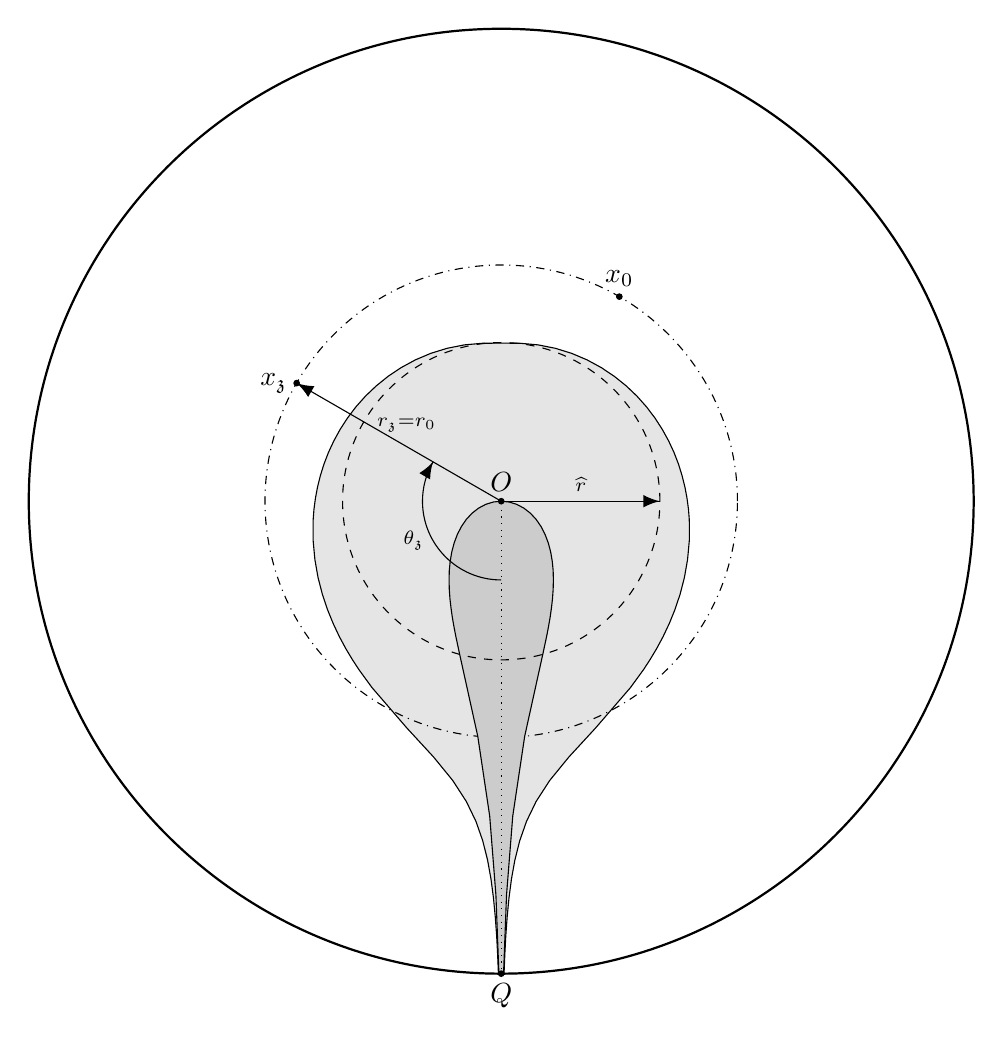
\begin{tikzpicture}[x=1cm,y=1cm,scale=0.5,
     decoration={
       markings,
       mark=at position 1 with {\arrow[scale=1.5,black]{latex}};
     }
   ]
      \def\c{12}
      \def\barr{4}
      \def\rrho{6}
      \def\radp{6}
      \def\phip{150}
      \def\phi0{60}
      \node[inner sep=0] (O) at (\c,\c) {};
      \node[inner sep=0] (P) at (2,4) {};
      \node[inner sep=0] (Q) at (\c,0) {};
      
      %\draw[gray!30,fill=gray!30] (O) circle (\barr);

      \draw[fill=black] (O) circle (0.035);

      \node[above] at (O) {$O$};
      %\draw[fill=black] (O) ++(\phip-360:\radp) circle (0.035);
      \draw[fill=black] (O) ++(\phi0-360:\radp) circle (0.07) node[above] {$x_0$};

      %\draw[postaction={decorate}] (O) -- node[midway,above] {$\widehat{r}$} ++(20:\barr);
      \draw[fill=gray!20] (11.929cm,0.000cm) -- (11.909cm,0.480cm) -- (11.884cm,0.961cm) -- (11.849cm,1.441cm) -- (11.803cm,1.922cm) -- (11.740cm,2.404cm) -- (11.653cm,2.887cm) -- (11.531cm,3.373cm) -- (11.359cm,3.865cm) -- (11.115cm,4.371cm) -- (10.769cm,4.906cm) -- (10.281cm,5.504cm) -- (9.604cm,6.239cm) -- (8.717cm,7.267cm) -- (8.385cm,7.723cm) -- (8.218cm,7.979cm) -- (8.051cm,8.258cm) -- (7.888cm,8.562cm) -- (7.732cm,8.892cm) -- (7.586cm,9.251cm) -- (7.456cm,9.640cm) -- (7.347cm,10.062cm) -- (7.267cm,10.518cm) -- (7.222cm,11.006cm) -- (7.223cm,11.527cm) -- (7.244cm,11.798cm) -- (7.281cm,12.076cm) -- (7.334cm,12.360cm) -- (7.406cm,12.648cm) -- (7.497cm,12.941cm) -- (7.610cm,13.235cm) -- (7.747cm,13.530cm) -- (7.908cm,13.823cm) -- (8.095cm,14.113cm) -- (8.309cm,14.396cm) -- (8.552cm,14.669cm) -- (8.825cm,14.929cm) -- (9.127cm,15.172cm) -- (9.459cm,15.394cm) -- (9.820cm,15.590cm) -- (10.209cm,15.755cm) -- (10.625cm,15.884cm) -- (11.065cm,15.971cm) -- (11.525cm,16.012cm) -- (12.000cm,16.015cm) -- (12.475cm,16.012cm) -- (12.935cm,15.971cm) -- (13.375cm,15.884cm) -- (13.791cm,15.755cm) -- (14.180cm,15.590cm) -- (14.541cm,15.394cm) -- (14.873cm,15.172cm) -- (15.175cm,14.929cm) -- (15.448cm,14.669cm) -- (15.691cm,14.396cm) -- (15.905cm,14.113cm) -- (16.092cm,13.823cm) -- (16.253cm,13.530cm) -- (16.390cm,13.235cm) -- (16.503cm,12.941cm) -- (16.594cm,12.648cm) -- (16.666cm,12.360cm) -- (16.719cm,12.076cm) -- (16.756cm,11.798cm) -- (16.777cm,11.527cm) -- (16.778cm,11.006cm) -- (16.733cm,10.518cm) -- (16.653cm,10.062cm) -- (16.544cm,9.640cm) -- (16.414cm,9.251cm) -- (16.268cm,8.892cm) -- (16.112cm,8.562cm) -- (15.949cm,8.258cm) -- (15.782cm,7.979cm) -- (15.615cm,7.723cm) -- (15.283cm,7.267cm) -- (14.396cm,6.239cm) -- (13.719cm,5.504cm) -- (13.231cm,4.906cm) -- (12.885cm,4.371cm) -- (12.641cm,3.865cm) -- (12.469cm,3.373cm) -- (12.347cm,2.887cm) -- (12.260cm,2.404cm) -- (12.197cm,1.922cm) -- (12.151cm,1.441cm) -- (12.116cm,0.961cm) -- (12.091cm,0.480cm) -- (12.071cm,0.000cm) -- (12.060cm,0.000cm) -- (12.045cm,0.000cm) -- (12.030cm,0.000cm) -- (12.015cm,0.000cm) -- (12.000cm,0.000cm) -- (11.985cm,0.000cm) -- (11.970cm,0.000cm) -- (11.955cm,0.000cm) -- (11.940cm,0.000cm) -- cycle;

      \draw[fill=black] (O) ++(\phip:\radp) circle (0.07);
      \draw[postaction={decorate}] (O) -- node[midway,above] {$\ \ _{r_{\ss}=r_0}$} ++(\phip:\radp) node[left] {$x_{\ss}$};
      \draw[dash dot] (O) circle (\rrho);
            
      \draw[fill=gray!40] (11.941cm,0.000cm) -- (11.865cm,2.001cm) -- (11.707cm,4.005cm) -- (11.404cm,6.030cm) -- (10.937cm,8.144cm) -- (10.842cm,8.591cm) -- (10.798cm,8.820cm) -- (10.758cm,9.051cm) -- (10.725cm,9.285cm) -- (10.698cm,9.521cm) -- (10.681cm,9.760cm) -- (10.675cm,9.999cm) -- (10.681cm,10.239cm) -- (10.704cm,10.477cm) -- (10.744cm,10.711cm) -- (10.804cm,10.938cm) -- (10.885cm,11.154cm) -- (10.988cm,11.356cm) -- (11.113cm,11.538cm) -- (11.260cm,11.696cm) -- (11.426cm,11.825cm) -- (11.608cm,11.921cm) -- (11.801cm,11.980cm) -- (12.000cm,12.000cm) --(12.199cm,11.980cm) -- (12.392cm,11.921cm) -- (12.574cm,11.825cm) -- (12.740cm,11.696cm) -- (12.887cm,11.538cm) -- (13.012cm,11.356cm) -- (13.115cm,11.154cm) -- (13.196cm,10.938cm) -- (13.256cm,10.711cm) -- (13.296cm,10.477cm) -- (13.319cm,10.239cm) -- (13.325cm,9.999cm) -- (13.319cm,9.760cm) -- (13.302cm,9.521cm) -- (13.275cm,9.285cm) -- (13.242cm,9.051cm) -- (13.202cm,8.820cm) -- (13.158cm,8.591cm) -- (13.063cm,8.144cm) -- (12.596cm,6.030cm) -- (12.293cm,4.005cm) -- (12.135cm,2.001cm) -- (12.059cm,0.000cm) -- (12.059cm,0.000cm) -- (12.045cm,0.000cm) -- (12.030cm,0.000cm) -- (12.015cm,0.000cm) -- (12.000cm,0.000cm) -- (11.985cm,0.000cm) -- (11.970cm,0.000cm) -- (11.955cm,0.000cm) -- (11.941cm,0.000cm) -- cycle;
      \draw[dotted] (O) -- (Q);
      \draw[dashed] (O) circle (4.03);
      \draw[postaction={decorate}] (O) -- node[midway,above] {$_{\widehat{r}}$} ++(0:4.03);
      \draw[postaction={decorate}] (\c,\c-2) arc (-90:\phip-360:2);
      \node at (\c-2.2,\c-1) {$_{\theta_{\ss}}$};
      \draw[thick] (O) circle (\c);
      \draw[fill=black] (Q) circle (0.07);
      \draw[fill=black] (O) circle (0.07);
      \node[below] at (Q) {$Q$};      
      \node[above] at (O) {$O$}; 
    \end{tikzpicture}
  \end{center}
  \caption{The position $x_{\ss}=(r_{\ss},\theta_{\ss})$ of particle $P$ at time
    $\ss$ is shown. The lightly shaded area corresponds to
    $\dt(\kappa)\setminus B_{Q}(R)$ and the strongly shaded
    region represents $B_Q(R)$. The dashed line corresponds to the arc
    segment where a particle $P$ at initial radial distance $r_0$ is,
    conditional under not having detected the target~$Q$ up to time
    $\ss$. The depicted dash-dot arc segment has length $C_{r_0}$.
    Each of the two dash-dot arc lengths inside the lightly shaded 
    region have (hyperbolic) length $\kappa\sqrt{\ss}$ corresponding to an angle $\theta_0$ such that
    $\phi(r_0)\leq |\theta_0| \le \phi(r_0)+\kappa \phi^{(\ss)}$.
    The dashed circle is the boundary of the largest ball centered at the origin which is contained in $\dt(\kappa)$.}\label{fig:angular}
\end{figure}

Following the proof strategy described in Section~\ref{sec:strategy}, we first define $\dt(\kappa)$. 
Recall that, roughly speaking, $\dt(\kappa)$ is the set of starting points from which a particle has a "good" chance to detect the target by time $\ss$, where "good" depends on a parameter $\kappa > 1$ (independent of $n$).
%Let $\ell_r$ denote the length of the perimeter of the ball $B_O(r)$ normalized by $2\pi$, that is, $\ell_{r}=\sinh(\beta r)$. 
Let $\phi^{(\ss)}$ be roughly proportional to the angular distance travelled by a particle at radial coordinate $r_0$ up to time $\ss$, more precisely, let $\phi^{(\ss)}:=\sqrt{\ss}e^{-\beta r_0}$ (that is,~$\phi^{(\ss)}$ corresponds to the standard deviation of a standard Brownian motion during an interval of time of length $\ss$ normalized by a term which is proportional to the perimeter of $B_O(r_0)$ for~$r_0$ bounded away from $0$). We can then define the following region (the shaded region in Figure~\ref{fig:angular}): %\cmk{About putting $\sqrt{s}/e^{\beta r}$ I kind of recalled that it was not a good idea because somewhere we then needed to approximate $\ell_{r}$ and added some asymptotic terms. In fact, I think that we might actually consider replacing the $\sqrt{\ss}/e^{\beta R}$ later by $\sqrt{\ss}/\ell_R$. Lets see.}\dmc{I saw that you changed a few, and I agree with them. But then it should probably also changed in the proof of the Lemma~\ref{lem:angular-muDt}, and then also in the statement, and also in the statement of the main theorem of this section. I first need to check whether indeed we need this approximation.}
\[
\dt = \dt(\kappa) := \big\{ x_0\in B_O(R) : |\theta_0| \le \phi(r_0)+\kappa \phi^{(\ss)}\big\}.
\]

In words, $\dt(\kappa)$ is the collection of points $x_0=(r_0,\theta_0)\in B_O(R)$ which are either contained in $B_Q(R)$ or form an angle at the origin of at most $\kappa \phi^{(\ss)}$ with a point that belongs to the boundary of $B_Q(R)$ and has radial coordinate exactly $r_0$.
Since $x_0\in B_{Q}(R)$ if and only if~$|\theta_0|\leq\phi(r_0)$, it is clear that $B_Q(R)$
is contained in $\dt(\kappa)$. The value $\kappa$ is a parameter that tells us at which scaling up to time $\ss$ we consider our region $\dt(\kappa)$. 

%\cmk{Changed statement below to make presentation consistent with strategy of proof section.}
The main goal of this section is to prove the result stated next
which is an instance of Theorem~\ref{thm:intro-Dt} for the case of angular movement only.
Thus, Theorem~\ref{thm:angularMain} will immediately follow  (by the proof strategy discussed in Section~\ref{sec:strategy}) once we show that~$\mu(\dt(\kappa))$ is of the right order:
\begin{theorem}\label{thm:mainangular}
Denote by $\Phi$ the standard normal distribution.
If $\kappa>0$ and 
  $\kappa\sqrt{\ss}\leq\frac{\pi}{2}(1-o(1))e^{\beta R}$, then
\[
\inf_{x_0\in\dt(\kappa)}\P_{x_0}(T_{det}\leq \ss)=\Omega(\Phi(-\kappa))
\qquad\text{and}\qquad
\sup_{x_0\in\ndt(\kappa)}\P_{x_0}(T_{det}\leq \ss)  = O(\Phi(-\kappa)).
\]
Furthermore,
\[
\int_{\ndt\!(\kappa)} \PP_{x_0}(T_{det}\le\ss)d\mu(x_0) = O(\mu(\dt(\kappa))).
\]
\end{theorem}
%\begin{theorem}\label{thm:mainangular}
%Let $\ss:=\ss(n)$. 
%If $\sqrt{\ss}\leq\frac{\pi}{2}(1-o(1))e^{\beta R}$, then  
%\[
%\P(T_{det}\geq \ss) = 
%\begin{cases}
%\exp\Big({-}\Theta\Big(\mkor{\nu}{1}+n\Big(\frac{\sqrt{\ss}}{e^{\beta R}}\Big)^{1\wedge \frac{\alpha}{\beta}}\Big)\Big), & \text{if $\alpha\neq\beta$,} \\[8pt]
%\exp\Big({-}\Theta\Big(\mkor{\nu}{1}+n\Big(\frac{\sqrt{\ss}}{e^{\beta R}}\Big)^{1\wedge \frac{\alpha}{\beta}}\log\big(\frac{e^{\beta R}}{1+\sqrt{\ss}}\big)\Big)\Big), & \text{if $\alpha=\beta$.}
%\end{cases}
%\]
%Furthermore, denote by $\Phi$ the standard normal distribution.
%If $\kappa>0$ and  $\kappa\sqrt{\ss}\leq\frac{\pi}{2}(1-o(1))e^{\beta R}$, then
%\[
%\inf_{x_0\in\dt(\kappa)}\P_{x_0}(T_{det}\leq \ss)=\Omega(\Phi(-\kappa))
%\qquad\text{and}\qquad
%\sup_{x_0\in\ndt(\kappa)}\P_{x_0}(T_{det}\leq \ss)  = O(\Phi(-\kappa)).
%\]
%\end{theorem}
%\cml{I think this is no longer true} In order to prove the previous result we will in fact separately establish even more detailed lower and upper bounds as the ones stated above. Theorem~\ref{thm:mainangular} will follow immediately from combining the mentioned bounds.

Before proving the previous result, we make a few observations and introduce some definitions. 
First, note that the perimeter of $B_{O}(r)$ that is outside $B_Q(R)$ has length (see Figure~\ref{fig:angular}) 
\[
C_{r}:=2(\pi-\phi(r))\sinh(\beta r).
\]
%Since, $\phi(r)\leq\phi(0)=\frac{\pi}{2}$ (by 
%Parts~\eqref{itm:phi2} and~\eqref{itm:phi3} of Lemma~\ref{lem:phi} ),
%\[\label{eqn:arcLengthBound}
%\tfrac12\pi e^{\beta r}(1-e^{-2\beta r})\leq C_r\leq \pi e^{\beta r}.
%\]


Since $\phi(\cdot)$ is decreasing and continuous 
(by Part~\eqref{itm:phi2} of Lemma~\ref{lem:phi}), 
we obtain the following:
\begin{fact}\label{fct:angular-monot}
The mapping $r\mapsto \frac12 C_r=(\pi-\phi(r))\sinh(\beta r)$ is increasing
and continuous for arguments in $[0,R]$ and takes values in $[0,\frac12 C_R]$.
\end{fact}
In particular, for  $\kappa\sqrt{\ss}\in [0,\frac12C_R]$ there is a unique value 
$\widehat{r}$ such that
\begin{equation}\label{eqn:angular-defrhat}
  \kappa\sqrt{\ss} = \tfrac12 C_{\widehat{r}}
    = (\pi-\phi(\widehat{r}))\sinh(\beta\widehat{r}).
\end{equation}
One may think of $\widehat{r}$ as chosen so that up to time $\kappa^2\ss$ a point at distance $\widehat{r}$ from the origin has a reasonable chance to detect the target due to their angular movement. Using Fact~\ref{fct:angular-monot}, we immediately obtain the following:
\begin{fact}\label{fct:angular-inclus}
For $r\in [0,R]$, the following holds:
$r\geq\widehat{r}$ if and only if $\kappa\sqrt{\ss}\leq\frac12 C_r$.
In particular, $B_O(\widehat{r})$ is the largest ball centered at the origin
contained in $\dt(\kappa)$.
\end{fact}
(See Figure~\ref{fig:angular} for an illustration of $B_O(\widehat{r})$.)
\begin{fact}\label{fct:angular-aproxhat} 
If $\widehat{r}>1$, then $\widehat{r}=\frac{1}{\beta}\log(\kappa\sqrt{\ss})+\Theta(1)$.
Moreover, if $\widehat{r}\leq 1$, then $\kappa\sqrt{\ss}=O(1)$.
\end{fact}
%Observe that $\kappa\sqrt{\ss}=\Omega(1)$ if and only if $\widehat{r}=\Omega(1)$ \cmk{Pending: Justify} and in this case $\kappa\sqrt{\ss}=\Theta(e^{\beta\widehat{r}})$. 
%Note also that all constants hidden inside the asymptotic notation are independent of $c$ (the approximation stemming from 
%the right hand side of~\eqref{eqn:sDef}). 

%Also, note that when bounding integrals over $\ndt$, for a given $r$, we may in fact assume that $\kappa\sqrt{\ss}\in [0,\frac12 C_r]$: indeed, if $\kappa\sqrt{\ss}> \frac12 C_r$, by definition of $\dt$, all of the boundary of $B_O(r)$ would be inside $\dt$, and hence when integrating over $\ndt$ for a given value of $r$, such a large value of $\ss$ would yield the empty set.
%\cmk{I could only find one place where the fact stated here is used. If so, rather than leaving this paragraph here, I would put it where its claim is used.}

%\subsection*{Angular motion: Lower bound.}
%
We will need the following claim whose proof is simple although the calculations involved are a bit tedious, mostly consisting in 
computing integrals and case analysis. 
\begin{lemma}\label{lem:angular-muDt}
If $\kappa>0$ and $\kappa\sqrt{\ss}\leq \frac{\pi}{2}(1-o(1))e^{\beta R}$, then
\[
\mu(\dt(\kappa))=
\begin{cases}
\Theta\Big(\mkor{\nu}{1}+n\Big(\frac{\kappa\sqrt{\ss}}{e^{\beta R}}\Big)^{1\wedge \frac{\alpha}{\beta}}\Big),
& \text{if $\alpha\neq\beta$,} \\[8pt]
\Theta\Big(\mkor{\nu}{1}+n\frac{\kappa\sqrt{\ss}}{e^{\beta R}}\Big(1+\log\big(\frac{e^{\beta R}}{\kappa\sqrt{\ss}}\big)\Big)\Big),
& \text{if $\alpha=\beta$.}
\end{cases}
\]
%\dmc{again would prefer to put the direct value}
%For the case where $\alpha=\beta$, the last identity holds with an additional $\log(\nnu^2/(\kappa\sqrt{\ss})^{\frac{1}{\beta}})$ factor 
%multiplying the second term inside the asymptotic notation.
\end{lemma}
\begin{proof}
If $\widehat{r}> R-\Theta(1)$, by~\eqref{eqn:angular-defrhat} and Part~\eqref{itm:phi3} of Lemma~\ref{lem:phi}, we see that $\kappa\sqrt{\ss}=\Theta(e^{\beta R})$ which always gives an expression of order $\Theta(n)$ on the right-hand side of the equality in the lemma's statement. On the other hand, by Fact~\ref{fct:angular-inclus}, we know that $B_O(\widehat{r})\subseteq\dt(\kappa)\subseteq B_O(R)$, so
from Lemma~\ref{lem:muBall} we get that $\mu(\dt(\kappa))=\Theta(\mu(B_O(\widehat{r})))=\Theta(n)$, and hence 
the claim holds for said large values of $\widehat{r}$.

Assume henceforth that $\widehat{r} \leq R-\Theta(1)$ and define $A:=\dt(\kappa)\setminus (B_Q(R)\cup B_O(\widehat{r}))$.
Clearly, 
\begin{equation}\label{eqn:angular-muSum}
\mu(\dt(\kappa)) = \mu(B_Q(R)\cup B_O(\widehat{r}))+\mu(A).
\end{equation}
Now, observe that $B_Q(R)$ is completely contained in half of the disk $B_O(R)$ (see Figure~\ref{fig:angular}), so
$\mu(B_Q(R)\cup B_O(\widehat{r}))=\mu(B_Q(R))+\Theta(\mu(B_O(\widehat{r})))$, and thus by Lemma~\ref{lem:muBall} and Fact~\ref{fct:angular-aproxhat}, for~$\widehat{r}>1$, 
\begin{equation}\label{eqn:angular-muNotA}
\mu(B_Q(R)\cup B_O(\widehat{r})))=\Theta\Big(n\Big(e^{-\frac{R}{2}}+\Big(\frac{\kappa\sqrt{\ss}}{e^{\beta R}}\Big)^{\frac{\alpha}{\beta}}\Big)\Big)
=\Theta\Big(\mkor{\nu}{1}+n\Big(\frac{\kappa\sqrt{\ss}}{e^{\beta R}}\Big)^{\frac{\alpha}{\beta}}\Big).
%\qquad\text{if $\widehat{r}>1$.}
\end{equation}
Moreover, the identity also holds when $\widehat{r}\leq 1$, since $\mu(B_Q(R))=\Theta(\mkor{\nu}{1})$ and $\mu(B_O(\widehat{r}))=O(ne^{-\alpha R})=o(1)$ (by Lemma~\ref{lem:muBall}, definition of $R$ and the fact that $\alpha>\frac12$), and $n(\kappa\sqrt{\ss}/e^{\beta R})^{\frac{\alpha}{\beta}}
=O(ne^{-\alpha R})=o(1)$ (by Fact~\ref{fct:angular-aproxhat}, definition of $R$ and since $\alpha>\frac12)$.


On the other hand, by Fact~\ref{fct:angular-inclus} and our choice of $\dt(\kappa)$, we get 
%\begin{equation}\label{eqn:angular-muA}
%\mu(A)= \Theta(ne^{-\alpha R})\int_{\widehat{r}}^R %\frac{\kappa\sqrt{\ss}}{\ell_{r_0}}\sinh(\alpha r_0)dr_0
%  = \Theta(ne^{-\alpha R}\kappa\sqrt{\ss})\int_{\widehat{r}}^R\frac{\sinh(\alpha r_0)}{\sinh(\beta r_0)}dr_0.
%\end{equation}
\begin{equation}\label{eqn:angular-muA}
\mu(A)= \Theta(ne^{-\alpha R}\kappa\sqrt{\ss})\int_{\widehat{r}}^R e^{-\beta r_0}\sinh(\alpha r_0)dr_0
%  = \Theta(ne^{-\alpha R}\kappa\sqrt{\ss})\int_{\widehat{r}}^R(e^{(\alpha-\beta)r_0}{-}e^{-(\alpha+\beta)r_0})dr_0.
\end{equation}
The next claim together with~\eqref{eqn:angular-muSum},  \eqref{eqn:angular-muNotA} and~\eqref{eqn:angular-muA} yield the lemma:
\[
ne^{-\alpha R}\kappa\sqrt{\ss}\int_{\widehat{r}}^R e^{-\beta r_0}\sinh(\alpha r_0)dr_0 =
\begin{cases}
O\Big(n\Big(\frac{\kappa\sqrt{\ss}}{e^{\beta R}}\Big)^{1\wedge \frac{\alpha}{\beta}}\Big),
& \text{if $\alpha\neq\beta$,} \\[8pt]
\Theta\Big(n\frac{\kappa\sqrt{\ss}}{e^{\beta R}}\log\big(\frac{e^{\beta R}}{\kappa\sqrt{\ss}}\big)\Big),
& \text{if $\alpha=\beta$.}
\end{cases}
\]
To prove the claim, not that when $\alpha=\beta$, the last integral equals $\Theta(R-\widehat{r})$.
If $\widehat{r}\leq 1$, by Fact~\ref{fct:angular-aproxhat} we have that $\kappa\sqrt{\ss}=O(1)$,
  so by definition of $R$ we get that $R-\widehat{r}=\Theta(R)=\Theta(\log(e^{\beta R}/(\kappa\sqrt{\ss})))$.
If on the other hand $\widehat{r}>1$, again by Fact~\ref{fct:angular-aproxhat}, we have that $\widehat{r}=\frac{1}{\beta}\log(\kappa\sqrt{\ss})+\Theta(1)$,
  so analogously to the previous calculations we obtain
  $R-\widehat{r}=\Theta(\log(e^{\beta R}/(\kappa\sqrt{\ss})))$.
Plugging back  establishes the claim when $\alpha=\beta$.  

For $\alpha > \beta$, since $\widehat{r}\leq R-\Theta(1)$, the claim follows 
because the integral therein
equals $\Theta(e^{(\alpha-\beta)R})$.
%Plugging this back into~\eqref{eqn:angular-muA} we see that $\mu(A)$ is of the right order and thus the claimed lower bound also holds when $\alpha>\beta$.
%Because of~\eqref{eqn:angular-muSum}, to obtain a matching upper bound for~$\mu(\dt(\kappa))$ it suffices to appropriately bound from above the right-hand side of~\eqref{eqn:angular-muNotA}. To do so, just note that since $\kappa\sqrt{\ss}\leq\frac{\pi}{2}e^{\beta R}$ and $\alpha>\beta$, we have that $(\kappa\sqrt{\ss}e^{-\beta R})^{\frac{\alpha}{\beta}} =O(\kappa\sqrt{\ss}e^{-\beta R})$.

Finally, when $\alpha<\beta$, the integral in the claim is
  $\Theta(e^{-(\beta-\alpha)\widehat{r}})$.
If $\widehat{r}>1$,  by Fact~\ref{fct:angular-aproxhat},
$e^{-(\beta-\alpha)\widehat{r}}
= \Theta((\kappa\sqrt{\ss})^{-(1-\frac{\alpha}{\beta})})$.
%Plugging this back into~\eqref{eqn:angular-muA} we obtain the desired upper bound on $\mu(A)$.
If $\widehat{r}\leq 1$, then $e^{-(\beta-\alpha)\widehat{r}}=O(1)$ and, again by Fact~\ref{fct:angular-aproxhat}, also $\kappa\sqrt{\ss}=O(1)$.
So, no matter the value of $\widehat{r}$ 
the claim holds when $\alpha<\beta$ which concludes the proof of the claim for all cases.
%Assume first $\alpha=\beta$. In this case the last integral equals $R-\widehat{r}$.
%If $\widehat{r}\leq 1$, by Fact~\ref{fct:angular-aproxhat} we have that $\kappa\sqrt{\ss}=O(1)$,
%  so by definition of $R$ we get that $R-\widehat{r}=\Theta(\log(e^{\beta R}/(\kappa\sqrt{\ss})))$.
%If on the other hand $\widehat{r}>1$, again by Fact~\ref{fct:angular-aproxhat}, we have that $\widehat{r}=\frac{1}{\beta}\log(\kappa\sqrt{\ss})+\Theta(1)$,  so analogously to the previous calculations we obtain   $R-\widehat{r}=\Theta(\log(e^{\beta R}/(\kappa\sqrt{\ss})))$.
%Plugging this back into~\eqref{eqn:angular-muA}, and then using~\eqref{eqn:angular-muSum} and~\eqref{eqn:angular-muNotA} 
%we obtain the claimed value for $\mu(\dt(\kappa))$ when $\alpha=\beta$.  
%
%Assume now $\alpha > \beta$. Then, the last integral in~\eqref{eqn:angular-muA} equals
%\[
%\int_{1\vee\widehat{r}}^1\frac{\sinh(\alpha r_0)}{\sinh(\beta r_0)}dr_0+\Theta(1)\int_{1\vee\widehat{r}}^{R}e^{(\alpha-\beta)r_0}dr_0 
%= \Theta(e^{(\alpha-\beta)R})
%\]
%because the first summand is either $0$ or $O(1)$ and where for the last equality we have used that $\widehat{r}\leq R-\Theta(1)$.
%Plugging this back into~\eqref{eqn:angular-muA} we see that $\mu(A)$ is of the right order and thus the claimed lower bound also holds when $\alpha>\beta$.
%Because of~\eqref{eqn:angular-muSum}, to obtain a matching upper bound for $\mu(\dt(\kappa))$  it suffices to appropriately bound from above the right-hand side of~\eqref{eqn:angular-muNotA}. 
%To do so, just note that since $\kappa\sqrt{\ss}\leq\frac{\pi}{2}e^{\beta R}$ and $\alpha>\beta$, we have that
%$(\kappa\sqrt{\ss}e^{-\beta R})^{\frac{\alpha}{\beta}}=O(\kappa\sqrt{\ss}e^{-\beta R})$.
%
%Finally, for the case where $\alpha<\beta$, by~\eqref{eqn:angular-muNotA} we see that $\mu(B_Q(R)\cup B_{O}(\widehat{r}))$ is of the right order and thus the claimed lower bound holds in this case as well. 
%Because of~\eqref{eqn:angular-muSum}, to obtain a matching upper bound for $\mu(\dt(\kappa))$, we need to establish the corresponding upper bound for $\mu(A)$.
%To do so, let us first consider the case where $\widehat{r}>1$. 
%Then, by Fact~\ref{fct:angular-aproxhat}, the last integral in~\eqref{eqn:angular-muA} now equals
%\[
%\int_{1\vee\widehat{r}}^1\frac{\sinh(\alpha r_0)}{\sinh(\beta r_0)}dr_0
%+ 
%\Theta(1)\int_{\widehat{r}}^Re^{-(\beta-\alpha)r_0}dr_0
%= \Theta(e^{-(\beta-\alpha)\widehat{r}})
%= \Theta((\kappa\sqrt{\ss})^{-(1-\frac{\alpha}{\beta})}).
%\]
%Plugging this back into~\eqref{eqn:angular-muA} we obtain the desired upper bound on $\mu(A)$.
%Consider next the case where $\widehat{r}\leq 1$. 
%Then, $\kappa\sqrt{\ss}=O(1)$ (by Fact~\ref{fct:angular-aproxhat}).
%Moreover, since $\alpha<\beta$, the last integral in~\eqref{eqn:angular-muA} is $O(1)$, so we get that $\mu(A)=O(ne^{-\alpha R})=o(1)$ (by definition of $R$ and given that~$\alpha>\frac12$).
%This completes the analysis of the case $\alpha<\beta$ and the proof for all cases.
\end{proof}

\medskip
We now have all the required ingredients to prove this section's main result.

\begin{proof}{(of Theorem~\ref{thm:mainangular})}
Throughout the ensuing discussion we let $\dt:=\dt(\kappa)$.
We begin by showing the uniform upper and lower bounds on $\P_{x_0}(T_{det}\leq \ss)$. To do so observe first that if $x_0\in B_Q(R)\subseteq \dt$, clearly $\P_{x_0} (T_{det} \le \ss)=1$ for any $\ss\ge0$ and hence the uniform lower bound follows directly for said $x_0$. Assume henceforth that $x_0\not\in B_Q(R)$ and observe that since there is only angular movement, a particle initially located at $(r_0,\theta_0)$ detects $Q$ if and only if it reaches $(r_0,\phi(r_0))$ or $(r_0,-\phi(r_0))$. Now, recall that the angular movement's
law is that of a variance $1$ Brownian motion $B_{\II{\ss}}$ with $\II{\ss}:=\int_{0}^{\ss} \cosech^2(\beta r_\ss)d\ss = (\phi^{(\ss)})^{2}$, so 
\begin{equation}\label{eqn:angular-exitt0}
\P_{x_0}(T_{det}\leq \ss)=\P(H_{[-a,b]}\leq \II{\ss})
\end{equation}
where we have used (with a slight abuse of notation) $\P$ for the law of a standard Brownian motion, and where $H_{[-a,b]}$ is its exit time from the interval $[-a,b]$ where in this case $a:=\phi(r_0)-|\theta_0|$ and $b:=2\pi-\phi(r_0)-|\theta_0|$. This last probability is a well studied function of~$a,b$ and $\II{\ss}$ (see~\cite{Borodin2002}, formula 3.0.2),
%This was written in more detail before, you left it out on purpose?}
which can be bounded using the reflection principle and the fact that~$a\leq b$, giving 
\begin{equation}\label{eqn:angular-exitt}
\P(H_{[-a,b]}\leq \II{\ss})=\Theta\big(\P(B_{\II{\ss}}\leq -a)\big)=\Theta\big(\Phi\big((\phi(r_0)-|\theta_0|)/\phi^{(\ss)}\big)\big).
\end{equation}
From our assumption $x_0\not\in B_Q(R)$ we deduce that $|\theta_0|>\phi(r_0)$, and hence the argument within~$\Phi$ above is always negative. It follows that for $\theta_0>0$ the mapping $\theta_0\mapsto\Phi\big((\phi(r_0)-\theta_0)/\phi^{(\ss)}\big)$ is decreasing, and so both uniform bounds on $\P_{x_0}(T_{det}\leq\ss)$ follow from the definition of $\dt(\kappa)$.

%To obtain the bound for $\P(T_{det}\geq \ss)$ recall that by~\eqref{eqn:main}
%\[\P(T_{det}\geq \ss)=\exp\Big(-\int_{\dt}\P_{x_0}(T_{det}\leq\ss)d\mu(x_0)-\int_{\ndt}\P_{x_0}(T_{det}\leq\ss)d\mu(x_0)\Big)\]
%for any $\kappa > 0$. Since for any $x_0\in\dt$ we have $\P_{x_0}(T_{det}\leq \ss)=\Omega(\Phi(-\kappa))$ it will be enough to take $\kappa=1$ to obtain that $\P_{x_0}(T_{det}\leq \ss)=\Theta(1)$, which gives $\int_{\dt}\P_{x_0}(T_{det}\leq\ss)d\mu(x_0)=\Theta(\mu(\dt))$, and hence it follows from Lemma~\ref{lem:angular-muDt} that this first term is already of the same order as the one in the theorem. Thus,  in order to conclude the theorem it only remains to prove that $\int_{\ndt}\P_{x_0}(T_{det}\leq\ss)d\mu(x_0)=O(\mu(\dt))$: 
We next establish the integral bound. Let $\dt:=\dt(\kappa)$.
%As observed in the discussion of our general strategy of proof (Section~\ref{sec:strategy}), given the uniform bounds just shown, to conclude it suffices to fix~$\kappa$, say $\kappa=1$, show that $\int_{\ndt}\P_{x_0}(T_{det}\leq\ss)d\mu(x_0)=O(\mu(\dt))$ and use Lemma~\ref{lem:angular-muDt}.
From~\eqref{eqn:angular-exitt0} and~\eqref{eqn:angular-exitt} we observe that
\begin{align*}
    \int_{\ndt}\P_{x_0}(T_{det}\leq\ss)d\mu(x_0)
    = \Theta(ne^{-\alpha R})\int_{\widehat{r}}^R\int_{\phi(r_0)+ \kappa\phi^{(\ss)}}^{\pi}\Phi\big((\phi(r_0)-\theta_0)/\phi^{(\ss)}\big)\sinh(\alpha r_0)d\theta_0dr_0.
\end{align*}
Applying the change of variables $y_0:=(\theta_0-\phi(r_0))/\phi^{(\ss)}$ and bounding $\pi$ by $\infty$ in the upper limit of the integral we obtain 
\begin{align*}
    \int_{\ndt}\P_{x_0}(T_{det}\leq\ss)d\mu(x_0)
    & = O(ne^{-\alpha R})\int_{\widehat{r}}^R\int_{\kappa}^{\infty}\Phi({-}y_0)\sinh(\alpha r_0)\phi^{(\ss)} dy_0dr_0 \\
    & =  O(ne^{-\alpha R}\sqrt{\ss})\int_{\widehat{r}}^R e^{-\beta r_0}\sinh(\alpha r_0)dr_0.
\end{align*}
The last expression is the same as one encountered in the proof of 
Lemma~\ref{lem:angular-muDt}. Substituting by the values obtained therein one gets a term which, by Lemma~\ref{lem:angular-muDt}, is $O(\mu(\dt(\kappa))$, thus completing the proof of the claimed integral upper bound.
\end{proof}

\section{Radial movement}\label{sec:radial}
%
The basic structure of this section is similar to Section~\ref{sec:angular}.
However, we now consider radial movement only. We define the relevant set $\dt:=\dt(\kappa)$ depending on a parameter $\kappa\geq 1$ independent of $n$, then we compute $\mu(\dt)$ and afterwards 
separately establish the stated upper and lower bounds. Since the radial movement contains a drift towards the boundary that makes the calculations more involved, we first need to prove basic results on such diffusion processes before actually defining $\dt$.
Let us thus start with the definition of the radial movement of a given particle, initially located at $x_0=(r_0, \theta_0)$. Recall that
a particle which at time~$\ss$ is in position
$x_s=(r_s,\theta_s)$ will stay at an angle $\theta_s=\theta_0$ while its
radial distance from the origin $r_s$ evolves according to a diffusion
process with a reflecting barrier at $R$ and generator 
\[
\Delta_{rad} := \frac{1}{2}\frac{\partial^2}{\partial r^2}+\frac{\alpha}{2}\frac{1}{\tanh(\alpha r)}\frac{\partial}{\partial r}.
\]
We are only concerned with the evolution of the process up until the detection time of the target, which occurs when the particle reaches $B_Q(R)$, and since the particles can only move radially, for any $x_0\not\in B_Q(R)$ we can also impose an absorbing barrier for $r_{s}$ at the radius $\rabs_0$ corresponding to the point in $\partial B_Q(R)$ with angle $\theta_0$. Recall that by Part~\eqref{itm:phiInv} of Lemma~\ref{lem:phi}, the function 
$\phi:[0,R]\to [\phi(R),\frac{\pi}{2}]$ has an inverse $\phi^{-1}$ 
which is also decreasing and continuous, so the absorbing barrier is given by $\rabs_0=\phi^{-1}(|\theta_0|)$.
This means that for values of $|\theta_0|>\frac{\pi}{2}$ we choose as absorbing barrier 
the origin $O$, that is,  $\rabs_0=0$.
Also recall that, whatever the value of $\theta_0$, we 
have that $(\theta_0,\rabs_0)$ always belongs to the boundary of $B_Q(R)$.
Since near the origin~$O$ the drift towards the boundary grows to infinity, for a point 
$x_0$ such that $|\theta_0|>\frac{\pi}{2}$ we have $\P_{x_0}(T_{det}\leq t)=0$ (in other words, at these angles the only way to detect $Q$ would be by reaching the origin, but since the drift there is $-\infty$ this is impossible). For the case where the absorbing barrier is distinct from the origin  we use the following result, which we state as a standalone result since it will be of use in later sections as well (by abuse of notation, since $\Delta_{rad}$ defined above depends only on the radial (one-dimensional) movement we use in the following lemma the operator $\Delta_{rad}$ also to denote the specific operator acting over sufficiently smooth one variable functions over the reals):%\dmc{the macros are good. The names I would change a bit, in this way it looks like $\auxY$ is a random variable, whereas $\yabs_0$ $\auxy$ is not. We'll see. Perhaps $\auxy=r$, $\yabs_0=\rho$, $\auxY=\rho'$?} 
\begin{lemma}\label{lemmaradial}
	Let $\{\auxy_s\}_{s\geq 0}$ be a diffusion process on $(0,\auxY]$ with generator $\Delta_{rad}$, and with a reflecting barrier at $\auxY$, and let $\P_{\auxy}$ denote the law of $\auxy_s$ with initial position $\auxy$. Define also $T_{\yabs_0}$, $T_\auxY$ the hitting times of~$\yabs_0$ and $\auxY$ respectively. We have:
	\begin{enumerate}[(i)]
	\item\label{radial:itm:phi1} For any $\lambda>0$ and any $\auxy\in[\yabs_0,\auxY]$,
	\begin{equation*}%\label{cotachern}
	\EE_{\auxy}(e^{-\lambda T_{\yabs_0}})\,\leq\,\frac{\lambda_1 e^{-\lambda_2 (\auxY-\auxy)}+\lambda_2 e^{\lambda_1(\auxY-\auxy)}}{{\lambda_1 e^{-\lambda_2 (\auxY-\yabs_0)}+\lambda_2 e^{\lambda_1(\auxY-\yabs_0)}}}\end{equation*}
	where $\lambda_1=\sqrt{\frac{\alpha^2}{4}+2\lambda}+\frac{\alpha}{2}$ and $\lambda_2=\sqrt{\frac{\alpha^2}{4}+2\lambda}-\frac{\alpha}{2}$.
	\item\label{radial:itm:phi2} If $\auxy\in[\yabs_0,\auxY]$, then
	\[\EE_{\auxy}(T_{\yabs_0})\,\leq\,\EE_{\auxY}(T_{\yabs_0})\,\leq\,\frac{e^{\alpha \auxY}}{\alpha^2}\log(\cotanh(\tfrac12\alpha \yabs_0)).\]
	In particular, if $\yabs_0>\tfrac{1}{\alpha}\log 2$, then 
	$\displaystyle
	\EE_{\auxy}(T_{\yabs_0})\,\leq\,\frac{4}{\alpha^2} e^{\alpha(\auxY-\yabs_0)}$.
	\item\label{radial:itm:phi3} If $\auxy\in[\yabs_0,\auxY]$, then
	\[G_{\yabs_0}(\auxy):=\PP_{\auxy}(T_{\yabs_0}<T_\auxY) = \frac{\log\big(\tfrac{\tanh(\alpha \auxY/2)}{\tanh(\alpha \auxy/2)}\big)}{\log\big(\tfrac{\tanh(\alpha \auxY/2)}{\tanh(\alpha \yabs_0/2)}\big)}.
	\]
	\item\label{radial:itm:phi4} If  $\auxy\in[\yabs_0,\auxY)$, then $\displaystyle
	\EE_{\auxy}(T_{\yabs_0}\,\big|\,T_{\yabs_0}<T_\auxY)\leq \frac{2}{\alpha}(\auxy-\yabs_0)+\frac{2}{\alpha^2}(1-G_{\yabs_0}(\auxy))$.
	\end{enumerate}
\end{lemma}
\begin{proof}
We begin with the proof of~\eqref{radial:itm:phi1} by observing that $\tanh(x)\leq 1$ for all positive values of~$x$ and hence we can couple the trajectory of a particle~$P$ with that of an auxiliary particle $\widetilde{P}$ starting with the same initial position as $P$, but whose radius $\widetilde{\auxy}_\ss$ evolves according to the diffusion with generator
\[
\widetilde{\Delta}_{rad}(f) := \frac{1}{2}f''+\frac{\alpha}{2}f',
\]
in such a way that $\widetilde{\auxy}_\ss\leq y_\ss$ for all $\ss$. It follows that the detection time $\widetilde{T}_{\yabs_0}$ of this auxiliary particle is smaller than the one of $P$ so in particular $\EE_{\auxy}(e^{-\lambda T_{\yabs_0}})\leq\EE_{\auxy}(e^{-\lambda \widetilde{T}_{\yabs_0}})$, and it suffices to prove the inequality for the auxiliary process. Let now $g$ be the solution of the following O.D.E.,
\begin{equation}\label{ODE1}
\frac{1}{2}g''(\auxy)+\frac{\alpha}{2}g'(\auxy)-\lambda g(\auxy)=0
\end{equation}
on $[\yabs_0,\auxY]$ with boundary conditions $g(\yabs_0)=1$ and $g'(\auxY)=0$, which is equal to
\[g(\auxy) = \frac{\lambda_1 e^{-\lambda_2 (\auxY-\auxy)}+\lambda_2 e^{\lambda_1(\auxY-\auxy)}}{{\lambda_1 e^{-\lambda_2 (\auxY-\yabs_0)}+\lambda_2 e^{\lambda_1(\auxy-\yabs_0)}}}\]
where $\lambda_1$ and $\lambda_2$ are as in the statement of the lemma. It follows from Itô's lemma that $\{e^{-\lambda s}g(\widetilde{\auxy}_s)\}_{s \ge 0}$ is a bounded martingale, and hence we can apply Doob's optional stopping theorem to deduce $g(\auxy)=\EE_{\auxy}(e^{-\lambda\cdot 0}g(\widetilde{\auxy}_0))=\EE_{\auxy}(e^{-\lambda\widetilde{T}_{\yabs_0}})$, giving the result. To obtain the bound in~\eqref{radial:itm:phi2}, we go back to the original process $\{\auxy_s\}_{s \ge 0}$ which evolves according to $\Delta_{rad}$, and define $F(\auxy)$ as the solution of the O.D.E. on $[\yabs_0,\auxY]$
\begin{equation}\label{eq(ii)}
-1 = \frac{1}{2}F''(\auxy)\,+\,\frac{\alpha}{2}\cotanh(\alpha \auxy)F'(\auxy)
\end{equation}
with boundary conditions $F'(\auxY)=0$ and $F(\yabs_0)=0$. We advance that the solution is smooth and bounded and deduce from Itô's lemma that $\{F(\auxy_s)+s\}_{s\ge 0}$ is a martingale, so applying Doob's optional stopping theorem we deduce $F(\auxy)=\EE_{\auxy}(F(\auxy_0)+0)=\EE_{\auxy}(F(\auxy_{t\wedge T_{\yabs_0}})+t\wedge T_{\yabs_0})$ for every $t>0$. Choosing any $c>0$, a simple argument obtained by restarting the process at $\auxY$ every $c$ units of time gives
\[\PP_\auxy(T_{\yabs_0}>t)\leq \PP_\auxY(T_{\yabs_0}>t)\leq(\PP_{\auxY}(T_{\yabs_0}>c))^{\lfloor\frac{t}{c}\rfloor},\]
and hence $\lim_{t\to\infty}t\PP_\auxy(T_{\yabs_0}>t)=0$. We deduce then that $\lim_{t\to\infty}\EE_\auxy(t\wedge T_{\yabs_0})=\EE_\auxy(T_{\yabs_0})$ and since $F$ is bounded, $\lim_{t\to\infty}\EE_{\auxy}(F(\auxy_{t\wedge T_{\yabs_0}})= \EE_{\auxy}(F(\auxy_{T_{\yabs_0}}))=0$. Thus, $F(\auxy)=\EE_\auxy(T_{\yabs_0})$, and it remains to solve the O.D.E. To do so, we  multiply~\eqref{eq(ii)} by $2\sinh(\alpha \auxy)$ to obtain
\[-2\sinh(\alpha \auxy) = \sinh(\alpha \auxy)F''(\auxy)+\alpha\cosh(\alpha \auxy)F'(\auxy) = (\sinh(\alpha \auxy)F'(\auxy))'.\]
Thus, integrating from $\auxy$ to $\auxY$ and using that $F'(\auxY)=0$ we have
\[\frac{2}{\alpha}(\cosh(\alpha \auxY)-\cosh(\alpha \auxy)) = \sinh(\alpha \auxy)F'(\auxy),\]
which in particular proves directly that $F(\auxy)$ is an increasing function, so that $\EE_{\auxy}(T_{\yabs_0})\leq \EE_\auxY(T_{\yabs_0})$. Integrating from $\yabs_0$ to $\auxY$, together with the condition $F'(\auxY)=0$ gives
%\cmk{The denominator inside the second $\log$ below should be $\tanh(\frac12\alpha\rabs_0)$, right?}\dmc{I get it in the numerator}
\[
\EE_\auxY(T_{\yabs_0}) = F(\auxY) = \frac{2}{\alpha^2}\Big(\log\Big(\frac{\sinh(\alpha \yabs_0)}{\sinh(\alpha \auxY)}\Big)-\cosh(\alpha \auxY)\log\Big(\frac{\tanh(\tfrac12\alpha\yabs_0)}{\tanh(\tfrac12\alpha \auxY)}\Big)\Big)
\]
and hence the general bound appearing in~\eqref{radial:itm:phi2} follows by noticing that the first term is negative, and by bounding $\cosh(\alpha \auxY)$ by $\frac{1}{2}e^{\alpha \auxY}$. To obtain $\EE_{\auxy}(T_{\yabs_0})\leq \frac{4}{\alpha^2} e^{\alpha(\auxY-\yabs_0)}$ observe that if we assume $\yabs_0>\tfrac{1}{\alpha}\log 2$ then $\cotanh(\tfrac12\alpha\yabs_0)\leq 1+4e^{-\alpha\yabs_0}$ so the result follows from bounding $\log(1+4e^{-\alpha\yabs_0})\leq4e^{-\alpha\yabs_0}$. 

To establish~\eqref{radial:itm:phi3} and~\eqref{radial:itm:phi4} it will be enough to work with a diffusion evolving on $(0,\infty)$ according to the original generator $\Delta_{rad}$, but without any barriers. Abusing notation we still call the process $\{\auxy_s\}_{s \ge 0}$. To deduce~\eqref{radial:itm:phi3}, observe that the solution of the O.D.E.
\[
0 = \frac{1}{2}G_{\rabs_0}''(\auxy) + \frac{\alpha}{2}\cotanh(\alpha \auxy)G_{\yabs_0}'(\auxy)
\]
with conditions $G_{\yabs_0}(\yabs_0)=1$ and $G_{\yabs_0}(\auxY)=0$ is given by the closed expression given in~\eqref{radial:itm:phi3}. It follows from Itô's lemma that $\{G_{\yabs_0}(\auxy_s)\}_{s \ge 0}$ is a bounded martingale, so applying Doob's optional stopping theorem we deduce $G_{\yabs_0}(y)=\EE_\auxy(G_{\yabs_0}(\auxy_0))=\EE_\auxy(G_{\yabs_0}(\auxy_{T_{\yabs_0}\wedge T_\auxY}))=\PP_{\auxy}(T_{\yabs_0}<T_\auxY)$.

Finally, to prove~\eqref{radial:itm:phi4} define the function $H(\auxy)$ as the solution of the ordinary differential equation
\[-G_{\yabs_0}(\auxy) = \frac{1}{2}H''(\auxy)\,+\,\frac{\alpha}{2}\cotanh(\alpha \auxy)H'(\auxy)\]
with boundary conditions $H(\yabs_0)=H(\auxY)=0$. It can be checked directly that the last equation is satisfied by
{\footnotesize
\begin{equation}\label{eq(iv)}
H(\auxy)=\frac{2}{\alpha}G_{\yabs_0}(r)\int_{\yabs_0}^{\auxy}\!\sinh(\alpha l)G_{\yabs_0}(l)\log\Big(\frac{\tanh(\frac{\alpha l}{2})}{\tanh(\frac{\alpha \yabs_0}{2})}\Big)dl+\frac{2}{\alpha}(1{-}G_{\yabs_0}(\auxy))\int_{\auxy}^\auxY\!\sinh(\alpha l)G_{\yabs_0}(l)\log\Big(\frac{\tanh(\frac{\alpha \auxY}{2})}{\tanh(\frac{\alpha l}{2})}\Big)dl,
\end{equation}}
which is smooth. It follows once again from Itô's lemma that $\{H(\auxy_s)+\int_0^s G_{\yabs_0}(\auxy_u)du\}_{s \ge 0}$ is a martingale. Since in the proof of~\eqref{radial:itm:phi3} we already showed that $\{G_{\yabs_0}(\auxy_s)\}_{s \ge 0}$ is a martingale, it follows that $\{\int_0^s G_{\yabs_0}(\auxy_u)du-s G_{\yabs_0}(\auxy_s)\}_{s \ge 0}$ is also a martingale. We conclude that $\{H(\auxy_s)+s G_{\yabs_0}(\auxy_s)\}_{s \ge 0}$ is a martingale, so applying Doob's optional stopping theorem we deduce
\[H(\auxy)=\EE_{\auxy}(H(\auxy_0)+0\cdot G_{\yabs_0}(y_0))=\EE_{\auxy}(H(\auxy_{t\wedge T_{\yabs_0}\wedge T_{\auxY}})+(t\wedge T_{\yabs_0}\wedge T_{\auxY})\cdot G_{\yabs_0}(\auxy_{t\wedge T_{\yabs_0}\wedge T_{\auxY}}))\]
for every $t>0$. Reasoning as in the proof of~\eqref{radial:itm:phi2} we can take the limit as $t\to\infty$ to obtain
\[H(\auxy)=\EE_{\auxy}(H(\auxy_{T_{\yabs_0}\wedge T_{\auxY}})+(T_{\yabs_0}\wedge T_{\auxY})\cdot G_{\yabs_0}(\auxy_{T_{\yabs_0}\wedge T_{\auxY}}))=\EE_{\auxy}(T_{\yabs_0}{\bf1}_{\{T_{\yabs_0}<T_{\auxY}\}})\]
where we used that $H(\yabs_0)=H(\auxY)=G_{\yabs_0}(\auxY)=0$ and $G_{\yabs_0}(\yabs_0)=1$. Observing that $\EE_{\auxy}(T_{\yabs_0}\,|\,T_{\yabs_0}<T_\auxY)=\frac{H(\auxy)}{G_{\yabs_0}(\auxy)}$, to obtain the inequality in~\eqref{radial:itm:phi4} we only need to bound $H(\auxy)$. To do so notice that for any $\yabs_0\leq l$ gives $\frac{\tanh(\alpha l/2)}{\tanh(\alpha \yabs_0/2)}\leq \frac{1}{\tanh(\alpha l/2)}$, which together with $0\leq G_{\yabs_0}(l)\leq 1$ allows us to bound from above the first integral of~\eqref{eq(iv)} by $\sinh(\alpha l)\log(\cotanh(\frac12\alpha l))=\frac{2\cotanh(\frac12\alpha l)}{\cotanh^2(\frac12\alpha l)-1}\log (\cotanh(\frac12\alpha l))=f(\cotanh(\frac12\alpha l))$, where $f(z)=\frac{2z}{z^2-1}\log z$ is bounded from above by $1$ on $[1,\infty)$. Using the same argument we can bound the term within the second integral of~\eqref{eq(iv)} by $G_{\yabs_0}(l)$, so that
\[\frac{H(\auxy)}{G_{\yabs_0}(\auxy)}\leq\frac{2}{\alpha}(\auxy-\yabs_0)+\frac{2}{\alpha}(1-G_{\yabs_0}(\auxy))\int_{\auxy}^\auxY \frac{G_{\yabs_0}(l)}{G_{\yabs_0}(\auxy)}dl.\]
Using the fact that $\frac{G_{\yabs_0}(l)}{G_{\yabs_0}(\auxy)}=G_{\auxy}(l)$, the second integral becomes $\int_{\auxy}^\auxY G_{\auxy}(l)dl$ which we control by studying the function $\auxy\mapsto \int_{\auxy}^\auxY G_{\auxy}(l)dl$ on $(0,\auxY)$. Notice first that any critical point $\auxy'$ of said function satisfies
\[\int_{\auxy'}^\auxY G_{\auxy'}(l)dl=\frac{1}{\alpha}\log\Big(\frac{\tanh(\frac12\alpha \auxY)}{\tanh(\frac12\alpha \auxy')}\Big)\sinh(\alpha \auxy')\leq\frac{1}{\alpha},\]
so it will be sufficient to control the integral when either $\auxy=\auxY$ or $\auxy=0$. For the first case we have $\int_{\auxY}^\auxY G_{\auxY}(l)dl=0$, and for the second one, by definition we have $\lim_{\auxy\to 0}G_{\auxy}(l)=0$ for any $l>0$. 
Since $G_\auxy(l)$ is monotone increasing in $\auxy$, by the monotone convergence theorem, $\lim_{\auxy\to 0}\int_\auxy^\auxY G_{\auxy}(l)dl=\int \lim_{\auxy \to 0} G_\auxy(l) dl=0$, so putting all these cases together we conclude $\int_\auxy^\auxY G_{\auxy}(l)dl\leq \frac{1}{\alpha}$.
\end{proof}

\medskip
Before we define $\dt(\kappa)$, let
\[
\phi^{(\ss)}:=\Big(\frac{\ss^{\frac{1}{\alpha}}}{e^{R}}\Big)^{\frac{1}{2}}.%+\phi(R).
\] 
Intuitively, one may think of $\phi^{(\ss)}$ as those points that are so close in terms of angle to the target, so that - even though possibly initially at the boundary of $B_O(R)$ - they have a reasonable chance to detect the target by time $\ss$ through the radial movement. %\dmc{If we put the definition of $\phi^{(\ss)}$ already in the angular section, and I think we should indeed as Marcos suggested, then perhaps also we should say the analogous thing there}\cmk{Yes. We should write $\phi^{(\ss)}=\ss^{\frac{1}{2\alpha}}/\ell_R$}\cmk{I looked at this again. Not sure we gain anything here by changing $e^{R/2}$ to $\ell_R=\sinh(R)$, in fact, it makes some calculations a bit harder to follow.}\dmc{Ok, let's switch it back then if you think}
We define~$\dt(\kappa)$ as the collection of points where a particle initially located can detect the target before time $\ss$ with a not too small probability (depending on $\kappa$). From our discussion preceding Lemma~\ref{lemmaradial}, we will always assume that any point $x_0\in\dt$ satisfies $|\theta_0|\leq\frac{\pi}{2}$. Since $\PP_{r}(T_{\rabs_0}<T_R)=G_{\rabs_0}(r)$, with $G_{\rabs_0}(r)$ as defined in Lemma~\ref{lemmaradial} with $y:=r$, $\yabs_0:=\rabs_0$ and $Y:=R$, it follows that $G_{\rabs_0}(r)$ is decreasing as a function of $r$, continuous and takes values in $[0,1]$. In particular, for $\kappa>1$ 
%\sout{The set $\dt$ will only contain points $x_0=(r_0,\theta_0)$
%such that $|\theta_0|\leq\frac{\pi}{2}$ (in particular $\dt$ 
%contains the origin $O$). 
%Unless explicitly said otherwise, for the ensuing discussion assume $x_0$ is such that %$|\theta_0|\leq\frac{\pi}{2}$. 
%Recall that by Part~\eqref{itm:phiInv} of Lemma~\ref{lem:phi}, the function 
%$\phi(\cdot):[0,R]\to [\phi(R),\frac{\pi}{2}]$ has an inverse $\phi^{-1}$ 
%which is also decreasing and continuous.
%Let $f$ be such that at $x_0=(r_0,\theta_0)\in\ndt$ with $\phi(R)< |\theta_0|<\frac{\pi}{2}$ %defined as} 
%\[
%\sout{f(r_0,\theta_0) = \frac{g(r_0)}{g(\phi^{-1}(|\theta_0|))}, \quad \text{ where } \quad
%g(r) =\log\Big(\frac{\tanh(\alpha R/2)}{\tanh(\alpha r/2)}\Big).}
%\]
%\sout{Clearly, when $\phi(r_0)=|\theta_0|$, we get that $f(r_0,\theta_0)=1$.
%%Thus, $f$ evaluates to $1$ at every point on the boundary of $B_{Q}(R)$.
%Also, when $r_0=R$, we have $f(r_0,\theta_0)=0$.
%Moreover, the mapping $r\mapsto g(r)/g(\phi^{-1}(|\theta_0|))$  
%from $[\phi^{-1}(|\theta_0|),R]$ to $[0,1]$ is continuous and decreasing.
%Henceforth, let $\rabs_0=\phi^{-1}(|\theta_0|)$ and, for the sake of convenience, let $\rabs_0=0$ %if $|\theta_0|\geq\frac{\pi}{2}$ (note that in this case $(\theta_0,\rabs_0)$ belongs to the 
%boundary of $B_Q(R)$ whatever the value taken by $\theta_0$).
%Henceforth, we always assume $\kappa>1$.
%From our ongoing discussion we conclude that for every $\ss\geq 0$} 
there is a unique $\widetilde{\rabs}_0\in [\rabs_0,R]$ such that
%\dmc{if we have $\kappa >1$ then we could directly into the formula (without defining $\delta$) put the right hand side of the equation below, and perhaps also put directly there $\Theta(\kappa^{-2\alpha})$}\cml{but this is not necessarily true if $\ss$ is small}
%\dmc{We'll finally have only values of $\ss$ at least being a large constant, in which case $\delta$ is a constant depending on $\kappa$. Maybe add a sentence something like "Note that by our lower bound on $\ss \ge C$ in Theorem~\ref{thm:radialmain}, we always have $\delta=\Theta(1)$, with the constant depending on $\kappa$". It would be good for the link with the main statement}
\begin{equation}\label{eqn:radial-defrtilde}
\PP_{\widetilde{\rabs}_0}(T_{\rabs_0}<T_R)=
\delta(\kappa,\ss), 
\quad\text{ where }\quad
\delta=\delta(\kappa,\ss):= \frac{1+\ss}{(1+\kappa\ss^{\frac{1}{2\alpha}})^{2\alpha}}.
\end{equation}
Note that $0\leq\delta(\kappa,\ss)< 1$ (the latter inequality holds because we assume $\kappa\geq 1$). Also observe that $\delta(\kappa,0)=1$ and $\delta(\kappa,\ss)$ tends to $\kappa^{-2\alpha}$ as $\ss$ tends to infinity.
Furthermore, $\delta(\kappa,\ss)=\Theta(\kappa^{-2\alpha})$ if $\ss=\Omega(1)$.
Now, define (see Figure~\ref{fig:radial}) 
\[
\dt = \dt(\kappa) := \big\{ x_0\in B_O(R) : |\theta_0|\leq\tfrac{\pi}{2} \wedge \big[|\theta_0|\leq\phi(R)+\kappa\phi^{(\ss)} \vee  r_0\leq\widetilde{\rabs}_0\big]\big\}.
\]
which contains $B_Q(R)$ since every $x_0\in B_Q(R)$ satisfies $r_0<\rabs_0\leq\widetilde{\rabs}_0$.
To better understand the motivation for defining $\widetilde{\rabs}_0$ and $\delta$ as above, we consider the most interesting regime, i.e.,~$\ss=\Omega(1)$. Under this condition the effect of the drift has enough time to move the particle far away from its initial position, and towards the boundary, so that the event $\{T_{\rabs_0}<\ss,\,T_{\rabs_0}<T_R\}$ is mostly explained by the particles' initial trajectory. In particular, by Part~\eqref{radial:itm:phi3} of Lemma~\ref{lemmaradial}, we have that $\PP_{r_0}(T_{\rabs_0}<\ss,\,T_{\rabs_0}<T_R)\approx \PP_{r_0}(T_{\rabs_0}<T_R)=G_{\rabs_0}(r_0)$,  so the condition $r_0\leq\widetilde{\rabs_0}$ aims to include in $\dt$ all points whose probability of detecting the target before reaching the boundary of $B_O(R)$ is not too small. To exhaust all possibilities, we must also include in $\dt$ all points which have a sufficiently large probability of detecting the target even after reaching the boundary of $B_O(R)$. Said points are considered through the condition $|\theta_0|\leq\phi(R)+\kappa\phi^{(\ss)}$, which gives a lower bound of order $\delta(\kappa,\ss)$ for the detection probability, thus explaining our choice of said function.
%\added[id=mk]{To better understand the motivation for defining $\widetilde{\rabs}_0$ as above, we consider the most interesting regime, i.e., $\ss=\Omega(1)$, for which as already observed, $\delta(\kappa,\ss)$ in terms of order only depends on $\kappa$ and controls the probability that a particle initially placed at $\widetilde{\rabs}_0$ detects $Q$ without ever having visited the boundary of $B_O(R)$. Giving the drift that the particle is subject to, the probability of detecting without visiting the boundary, i.e.,~$\PP_{\widetilde{\rabs}_0}(T_{\rabs_0}<T_R)$, is mostly explained by the initial trajectory of the particle, thence mostly independent of $\ss$ for all but very small values of $\ss$ \dmc{should we rather say: it is mostly independent of $\ss$, as long as $\ss = \Omega(1)$ ? See the new remark also below}. Moreover, by Part~\eqref{radial:itm:phi3} of Lemma~\ref{lemmaradial}, we know that $\PP_{\widetilde{\rabs}_0}(T_{\rabs_0}<T_R)=G_{\rabs_0}(\widetilde{\rabs}_0)$ and can thus estimate $\widetilde{\rabs}_0$ as a function of $\delta$.\dmc{here I would prefer also to say just as a function of $\kappa$, but I won't insist}}

\medskip
Before moving to the main theorem of this section, we spend some time building some intuition about the geometric shape of $\dt$. 
Since $\rabs_0$ goes to $0$ when $\theta_0$ tends to $\frac{\pi}{2}$, from~\eqref{eqn:radial-defrtilde} which is used to define $\widetilde{\rabs}_0$, it is not hard to see that 
$\widetilde{\rabs}_0$ also goes to $0$
(and hence $\widetilde{\rabs}_0-\rabs_0$ as well) when $\theta_0$ tends to $\frac{\pi}{2}$.
It requires a fair amount of additional work to show that $\widetilde{\rabs}_0-\rabs_0$, as a function of $\theta_0>\phi(R)+\kappa\phi^{(\ss)}$, first increases very slowly, then reaches a maximum value of roughly $\frac{1}{\alpha}\log\frac{1}{\delta}$
and finally decreases rapidly (we omit the details since we will not rely on this observation). In fact, for all practical purposes, one might think of $\widetilde{\rabs}_0-\rabs_0$ as being essentially constant up to the point when $\rabs_0$ is smaller than a constant (equivalently, $\theta_0$ is at least a constant).

%\cmk{Changed statement to make presentation consistent with strategy of proof.}\dmc{Ok for me}
The main goal of this section is to prove the following result from which Theorem~\ref{thm:radialmain} immediately follows (by the proof strategy discussed in Section~\ref{sec:strategy}) once we show that~$\mu(\dt(\kappa))$ is of the right order:
\begin{theorem}\label{thm:rad} 
The following hold:
\begin{enumerate}[(i)]
\item If $\kappa\geq 1$ and $\phi(R)+\kappa\phi^{(\ss)}\leq \frac{\pi}{2}$, then $\sup_{x_0 \in \ndt}\PP_{x_0}(T_{det}\leq\ss)=O(\delta(\kappa,\ss))$ and
\[
\int_{\ndt\!(\kappa)}\P(T_{det}\leq\ss)d\mu(x_0) = O(\mu(\dt(\kappa))). 
\]
\item\label{thm:rad:itm2} For every $c>0$ there is a $\kappa_0 >0$ such that if $\kappa\ge\kappa_0$ and $\ss= \frac{16}{\alpha}\log \kappa+\Omega(1)$ satisfy $\phi(R)+\kappa\phi^{(\ss)}\leq \frac{\pi}{2}-c$, then $\inf_{x_0 \in \dt}\PP_{x_0}(T_{det}\leq\ss)=\Omega(\delta(\kappa,\ss))$.
\end{enumerate}
\end{theorem}


\begin{comment}
\begin{remark}
The upper bound on $\ss$ implicit in the hypothesis $\phi(R)+\phi^{(\ss)}\leq\frac{\pi}{2}$ stems from the fact that for $\ss > \frac{\pi}{2}e^{\alpha R}$ 
the first probability of the above theorem is $e^{-\Omega(n)}$. The same conclusion follows from the fact that having zero points in a Poisson point process of intensity $n$ occurs with probability $e^{-\Theta(n)}$, hence for such values of $\ss$ the upper bound becomes trivial.
\end{remark}
\end{comment} 

\begin{remark}
The extra hypotheses on $\kappa$ and $\ss$ needed for the lower bounds of Part~\eqref{thm:rad:itm2} of Theorem~\ref{thm:rad} %\sout{$\PP_{x_0}(T_{det}\leq\ss)$ and $\dt$}\cmk{It is unclear what we mean by "and $\dt$". Needs to be clarified}\dmc{Just leave out?} 
are key for our methods to work, %since for small times $\ss$ the probability of a particle travelling too far is exponentially \sout{low} \dm{small}. 
since for small times $\ss= o(1)$ the detection probability for a point always tends to $0$ unless it is already in $B_Q(R)$ or very close to it (but the latter set is of smaller measure than $B_Q(R)$). Similarly, if one is very close to the origin (that is, for angles very close to $\frac{\pi}{2}$) the explosion of the drift towards the boundary at the origin also implies an extra penalization for the probability of detection. Observe nevertheless that the extra hypothesis in Part~\eqref{thm:rad:itm2} are automatically satisfied if $\ss=\omega(1)\cap o(e^{\alpha R})$.
Furthermore, the hypothesis $\ss =\Omega(1)$ is natural since in the case of radial movement only we will show that $\EE(T_{det})=\Theta(1)$, and we are interested in tail behaviors of the detection time.
\end{remark}

%\dmc{So the next remark is now removed I guess by adding your previous remark Amitai, I guess}\cml{maybe, although mine focuses on the hypotheses on $\kappa$, maybe we should mention the consequences on $\ss$?}

%\dm{
%\begin{remark}
%The hypothesis of $\ss =\Omega(1)$ is natural \deleted[id=mk]{(to us)} for the following reasons: on the one hand, since in the case of radial movement only we have $\EE(T_{det})=\Theta(1)$, and we are interested in tail behaviors of the detection time. On the other hand, if $\ss=o(1)$, with probability tending to $1$ the radius does not change by more than a $o(1)$, and so detection cannot be significantly higher than in the static case where $\dt=B_Q(R)$ (of course if one is very close to the origin, there is a stronger drift towards the boundary, but in this case either the particle is already in $B_Q(R)$ or it is rather pushed in the opposite direction, and it is again as the static case).
%\end{remark}}



Among all facts regarding the intuition of $\dt$, we will only need to prove rigorously (see the next result) that if $\phi(R)+\kappa\phi^{(\ss)}\leq |\theta_0|\leq\frac{\pi}{2}$, then $\widetilde{\rabs}_0-\rabs_0\leq\frac{1}{\alpha}\log\frac{1}{\delta}+O(1)$.
\begin{fact}\label{fct:radial-varphi2}
For $\ss> 0$ and $\kappa\geq 1$, 
if $\theta_0\in [\phi(R)+\kappa\phi^{(\ss)},\frac{\pi}{2}]$, then
  $e^{\widetilde{\rabs}_0-\rabs_0}=O(1/\delta^{\frac{1}{\alpha}})$
  where $\delta:=\delta(\kappa,\ss)$.
\end{fact}
\begin{proof}
We first handle some simple cases.
If $\widetilde{\rabs}_0\leq\frac{1}{\alpha}\log\frac{2}{\delta}$, then $e^{\widetilde{r}_0-\rabs_0}\leq e^{\widetilde{r}_0}\leq (2/\delta)^{\frac{1}{\alpha}}$ and we are done.
Similarly, if $\rabs_0\geq R-\frac{1}{\alpha}\log\frac{3}{\delta}$, since $\widetilde{\rabs}_0\leq R$, we have that $e^{\widetilde{r}_0-\rabs_0}\leq e^{R-\rabs_0}\leq (3/\delta)^{\frac{1}{\alpha}}$ and we obtain again the claimed bound. Henceforth, assume that $\widetilde{\rabs}_0>\frac{1}{\alpha}\log\frac{2}{\delta}$ and that $\rabs_0< R-\frac{1}{\alpha}\log\frac{3}{\delta}$.

Let $g(r):=\log(\tanh(\frac12\alpha R)/\tanh(\frac12\alpha r))$ and note that since $\tanh(x)\leq 1$, $\cotanh(x)=1+\frac{2e^{-2x}}{1-e^{-2x}}$ and $1+y\leq e^{y}$, 
\[g(\widetilde{\rabs}_0) \leq \log(\cotanh(\tfrac12\alpha\widetilde{\rabs}_0))
\leq\frac{2e^{-\alpha\widetilde{\rabs}_0}}{1-e^{-\alpha\widetilde{\rabs}_0}}\leq4e^{-\alpha\widetilde{\rabs}_0},\]
where in the last inequality we have used that $\delta\leq 1$. Moreover, since $\tanh(x)=1-\frac{2e^{-2x}}{1+e^{-2x}}$, 
$\cotanh(x)=1+\frac{2e^{-2x}}{1-e^{-2x}}$ and
using twice that $\log(1+y)\geq \frac{y}{1+y}$ for $y>-1$, we have
\[
g(\rabs_0) = \log(\coth(\tfrac12\alpha\rabs_0))+\log(\tanh(\tfrac12\alpha R)) \geq \frac{2e^{-\alpha\rabs_0}}{1+e^{-\alpha\rabs_0}} - 
\frac{2e^{-\alpha R}}{1-e^{-\alpha R}}
\geq e^{-\alpha\rabs_0}-(2+o(1))e^{-\alpha R}.
\]
Since $\delta\leq 1$, by our assumption on $\rabs_0$, we conclude that
  $g(\rabs_0)=\Omega(e^{-\alpha\rabs_0})$. Observing that $g(\widetilde{\rabs}_0)/g(\rabs_0)=G_{\rabs_0}(\widetilde{\rabs}_0)=\delta$, it follows from the 
previously derived bounds on $g(\widetilde{\rabs}_0)$ and $g(\rabs_0)$ 
that $e^{\alpha(\widetilde{\rabs}_0-\rabs_0)}=O(\delta^{-1})$ 
and thus $e^{\widetilde{\rabs}_0-\rabs_0}=O(1/\delta^{\frac{1}{\alpha}})$ as desired.
\end{proof}
For practical purposes one may view $\dt$ as the collection of points of $B_O(R)$
which belong either to a sector of angle $2(\phi(R)+\kappa\phi^{(\ss)})$ 
whose bisector contains $Q$, 
or to the ball $B_Q(R)$, or to those points with angular coordinate $|\theta_0|\geq \phi(R)+\kappa\phi^{(\ss)}$ which are 
within radial distance roughly $\frac{1}{\alpha}\log\frac{1}{\delta}$ of $B_Q(R)$. 
This picture would be accurate except for the fact that it places into $\dt$ points with angular coordinate close to $\frac{\pi}{2}$ and fairly close to the origin $O$, say at distance 
$\frac{1}{\alpha}\log\frac{1}{\delta}-\Omega(1)$. 
However, particles initially located at such points are extremely unlikely to reach $B_Q(R)$ and detect $Q$, since the drift towards the boundary tends to infinity close to the origin.
This partly justifies why $\dt$ is defined so that in the case where $\theta_0$ goes to $\frac{\pi}{2}$ the expression $\widetilde{\rabs}_0-\rabs_0$ tends to $0$, thus 
leaving out of $\dt$ the previously mentioned problematic points.


\begin{figure}
\begin{center}
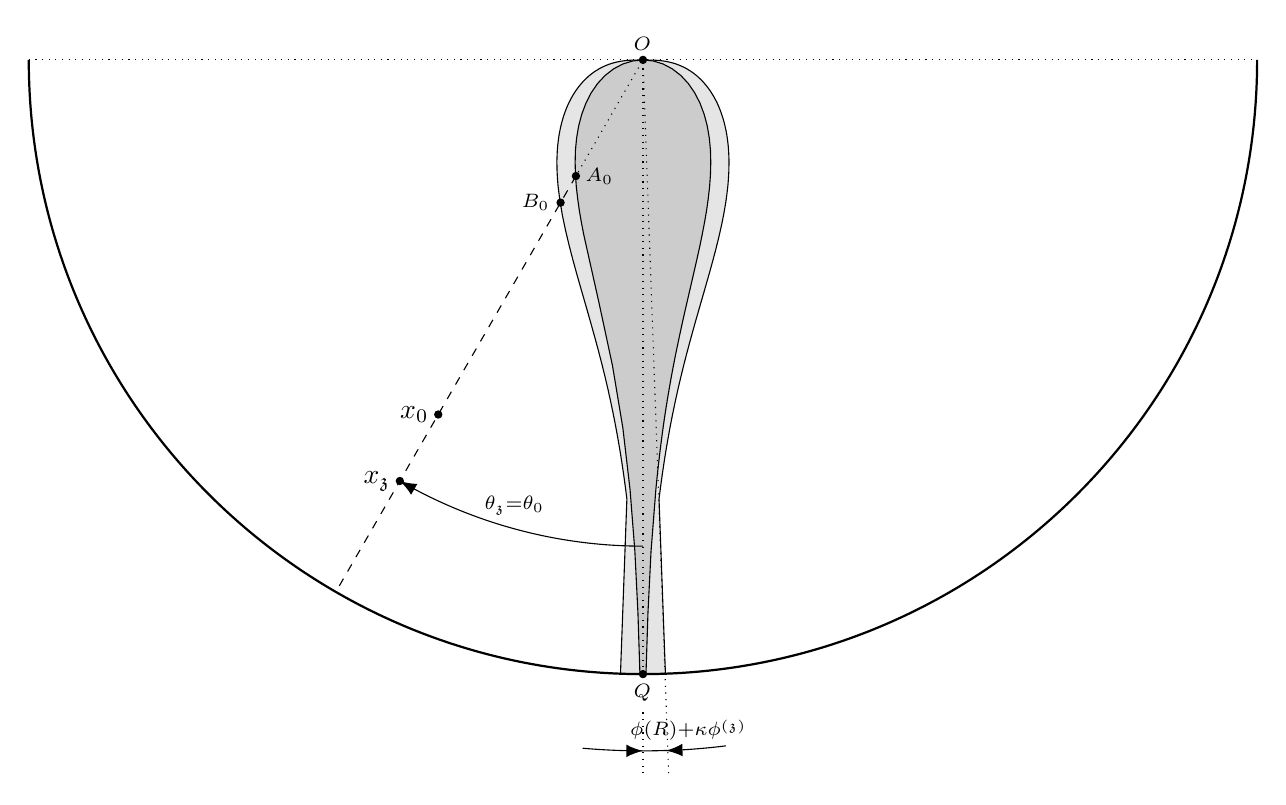
\begin{tikzpicture}[x=1cm,y=1cm,scale=0.65,
     decoration={markings,
       mark=at position 1 with {\arrow[scale=1.5,black]{latex}};
      }]
      
      \def\c{12}
      \def\barr{4}
      \def\radp{9.5}
      \def\phip{240}
      \def\angabs{-87.94}
      \node[inner sep=0] (O) at (\c,\c) {};
      \node[inner sep=0] (P) at (2,4) {};
      \node[inner sep=0] (Q) at (\c,0) {};
  \draw[fill=gray!20] (11.561cm,0.008cm) --(11.686cm,3.423cm) -- (11.656cm,3.656cm) -- (11.624cm,3.891cm) -- (11.589cm,4.126cm) -- (11.552cm,4.362cm) -- (11.511cm,4.599cm) -- (11.468cm,4.837cm) -- (11.421cm,5.076cm) -- (11.371cm,5.316cm) -- (11.318cm,5.558cm) -- (11.261cm,5.800cm) -- (11.201cm,6.045cm) -- (11.137cm,6.291cm) -- (11.070cm,6.540cm) -- (11.000cm,6.792cm) -- (10.928cm,7.047cm) -- (10.854cm,7.305cm) -- (10.778cm,7.568cm) -- (10.702cm,7.835cm) -- (10.627cm,8.108cm) -- (10.555cm,8.387cm) -- (10.487cm,8.672cm) -- (10.426cm,8.963cm) -- (10.376cm,9.261cm) -- (10.344cm,9.513cm) -- (10.339cm,9.563cm) -- (10.335cm,9.614cm) -- (10.331cm,9.665cm) -- (10.328cm,9.717cm) -- (10.325cm,9.768cm) -- (10.322cm,9.819cm) -- (10.321cm,9.870cm) -- (10.320cm,9.922cm) -- (10.319cm,9.973cm) -- (10.319cm,10.025cm) -- (10.320cm,10.076cm) -- (10.322cm,10.128cm) -- (10.324cm,10.179cm) -- (10.327cm,10.231cm) -- (10.331cm,10.282cm) -- (10.335cm,10.333cm) -- (10.341cm,10.384cm) -- (10.347cm,10.435cm) -- (10.354cm,10.486cm) -- (10.362cm,10.537cm) -- (10.371cm,10.587cm) -- (10.381cm,10.638cm) -- (10.392cm,10.688cm) -- (10.403cm,10.737cm) -- (10.416cm,10.787cm) -- (10.430cm,10.836cm) -- (10.444cm,10.884cm) -- (10.460cm,10.932cm) -- (10.477cm,10.980cm) -- (10.494cm,11.027cm) -- (10.513cm,11.074cm) -- (10.533cm,11.120cm) -- (10.554cm,11.166cm) -- (10.577cm,11.211cm) -- (10.600cm,11.255cm) -- (10.625cm,11.299cm) -- (10.651cm,11.341cm) -- (10.678cm,11.383cm) -- (10.706cm,11.424cm) -- (10.736cm,11.465cm) -- (10.767cm,11.504cm) -- (10.799cm,11.542cm) -- (10.832cm,11.579cm) -- (10.867cm,11.615cm) -- (10.904cm,11.650cm) -- (10.941cm,11.684cm) -- (10.981cm,11.717cm) -- (11.022cm,11.748cm) -- (11.065cm,11.778cm) -- (11.110cm,11.806cm) -- (11.156cm,11.834cm) -- (11.205cm,11.859cm) -- (11.257cm,11.883cm) -- (11.311cm,11.905cm) -- (11.369cm,11.926cm) -- (11.431cm,11.944cm) -- (11.499cm,11.961cm) -- (11.574cm,11.975cm) -- (11.660cm,11.987cm) -- (11.769cm,11.995cm) -- (12.000cm,12.000cm) --(12.231cm,11.995cm) -- (12.340cm,11.987cm) -- (12.426cm,11.975cm) -- (12.501cm,11.961cm) -- (12.569cm,11.944cm) -- (12.631cm,11.926cm) -- (12.689cm,11.905cm) -- (12.743cm,11.883cm) -- (12.795cm,11.859cm) -- (12.844cm,11.834cm) -- (12.890cm,11.806cm) -- (12.935cm,11.778cm) -- (12.978cm,11.748cm) -- (13.019cm,11.717cm) -- (13.059cm,11.684cm) -- (13.096cm,11.650cm) -- (13.133cm,11.615cm) -- (13.168cm,11.579cm) -- (13.201cm,11.542cm) -- (13.233cm,11.504cm) -- (13.264cm,11.465cm) -- (13.294cm,11.424cm) -- (13.322cm,11.383cm) -- (13.349cm,11.341cm) -- (13.375cm,11.299cm) -- (13.400cm,11.255cm) -- (13.423cm,11.211cm) -- (13.446cm,11.166cm) -- (13.467cm,11.120cm) -- (13.487cm,11.074cm) -- (13.506cm,11.027cm) -- (13.523cm,10.980cm) -- (13.540cm,10.932cm) -- (13.556cm,10.884cm) -- (13.570cm,10.836cm) -- (13.584cm,10.787cm) -- (13.597cm,10.737cm) -- (13.608cm,10.688cm) -- (13.619cm,10.638cm) -- (13.629cm,10.587cm) -- (13.638cm,10.537cm) -- (13.646cm,10.486cm) -- (13.653cm,10.435cm) -- (13.659cm,10.384cm) -- (13.665cm,10.333cm) -- (13.669cm,10.282cm) -- (13.673cm,10.231cm) -- (13.676cm,10.179cm) -- (13.678cm,10.128cm) -- (13.680cm,10.076cm) -- (13.681cm,10.025cm) -- (13.681cm,9.973cm) -- (13.680cm,9.922cm) -- (13.679cm,9.870cm) -- (13.678cm,9.819cm) -- (13.675cm,9.768cm) -- (13.672cm,9.717cm) -- (13.669cm,9.665cm) -- (13.665cm,9.614cm) -- (13.661cm,9.563cm) -- (13.656cm,9.513cm) -- (13.650cm,9.462cm) -- (13.644cm,9.411cm) -- (13.638cm,9.361cm) -- (13.631cm,9.311cm) -- (13.624cm,9.261cm) -- (13.617cm,9.211cm) -- (13.609cm,9.161cm) -- (13.600cm,9.111cm) -- (13.592cm,9.062cm) -- (13.583cm,9.012cm) -- (13.574cm,8.963cm) -- (13.564cm,8.914cm) -- (13.555cm,8.865cm) -- (13.545cm,8.817cm) -- (13.534cm,8.768cm) -- (13.524cm,8.720cm) -- (13.513cm,8.672cm) -- (13.502cm,8.624cm) -- (13.491cm,8.576cm) -- (13.480cm,8.529cm) -- (13.469cm,8.481cm) -- (13.457cm,8.434cm) -- (13.445cm,8.387cm) -- (13.434cm,8.340cm) -- (13.422cm,8.293cm) -- (13.410cm,8.247cm) -- (13.398cm,8.200cm) -- (13.385cm,8.154cm) -- (13.373cm,8.108cm) -- (13.361cm,8.062cm) -- (13.348cm,8.017cm) -- (13.336cm,7.971cm) -- (13.323cm,7.926cm) -- (13.311cm,7.880cm) -- (13.298cm,7.835cm) -- (13.285cm,7.790cm) -- (13.273cm,7.746cm) -- (13.260cm,7.701cm) -- (13.247cm,7.657cm) -- (13.235cm,7.612cm) -- (13.222cm,7.568cm) -- (13.209cm,7.524cm) -- (13.197cm,7.480cm) -- (13.184cm,7.436cm) -- (13.171cm,7.392cm) -- (13.159cm,7.349cm) -- (13.146cm,7.305cm) -- (13.134cm,7.262cm) -- (13.121cm,7.219cm) -- (13.109cm,7.175cm) -- (13.096cm,7.132cm) -- (13.084cm,7.090cm) -- (13.072cm,7.047cm) -- (13.060cm,7.004cm) -- (13.047cm,6.961cm) -- (13.035cm,6.919cm) -- (13.023cm,6.876cm) -- (13.011cm,6.834cm) -- (13.000cm,6.792cm) -- (12.988cm,6.750cm) -- (12.976cm,6.708cm) -- (12.964cm,6.666cm) -- (12.953cm,6.624cm) -- (12.941cm,6.582cm) -- (12.930cm,6.540cm) -- (12.918cm,6.499cm) -- (12.907cm,6.457cm) -- (12.896cm,6.416cm) -- (12.885cm,6.374cm) -- (12.874cm,6.333cm) -- (12.863cm,6.291cm) -- (12.852cm,6.250cm) -- (12.841cm,6.209cm) -- (12.831cm,6.168cm) -- (12.820cm,6.127cm) -- (12.810cm,6.086cm) -- (12.799cm,6.045cm) -- (12.789cm,6.004cm) -- (12.779cm,5.963cm) -- (12.769cm,5.922cm) -- (12.759cm,5.882cm) -- (12.739cm,5.800cm) -- (12.682cm,5.558cm) -- (12.629cm,5.316cm) -- (12.579cm,5.076cm) -- (12.532cm,4.837cm) -- (12.489cm,4.599cm) -- (12.448cm,4.362cm) -- (12.411cm,4.126cm) -- (12.376cm,3.891cm) -- (12.344cm,3.656cm) -- (12.314cm,3.423cm) -- (12.439cm,0.008cm) --(12.352cm,0.005cm) --(12.264cm,0.003cm) --(12.176cm,0.001cm) --(12.088cm,0.000cm) --(12.000cm,0.000cm) --(11.912cm,0.000cm) --(11.824cm,0.001cm) --(11.736cm,0.003cm) --(11.648cm,0.005cm) --(11.561cm,0.008cm) --(12.439cm,0.008cm) --cycle;

\draw[fill=gray!40] (11.941cm,0.000cm) -- (11.902cm,1.200cm) -- (11.842cm,2.401cm) -- (11.748cm,3.604cm) -- (11.607cm,4.811cm) -- (11.404cm,6.030cm) -- (11.136cm,7.278cm) -- (10.842cm,8.591cm) -- (10.798cm,8.820cm) -- (10.758cm,9.051cm) -- (10.725cm,9.285cm) -- (10.698cm,9.521cm) -- (10.681cm,9.760cm) -- (10.675cm,9.999cm) -- (10.681cm,10.239cm) -- (10.704cm,10.477cm) -- (10.744cm,10.711cm) -- (10.804cm,10.938cm) -- (10.885cm,11.154cm) -- (10.988cm,11.356cm) -- (11.113cm,11.538cm) -- (11.260cm,11.696cm) -- (11.426cm,11.825cm) -- (11.608cm,11.921cm) -- (11.801cm,11.980cm) -- (12.000cm,12.000cm) --(12.199cm,11.980cm) -- (12.392cm,11.921cm) -- (12.574cm,11.825cm) -- (12.740cm,11.696cm) -- (12.887cm,11.538cm) -- (13.012cm,11.356cm) -- (13.115cm,11.154cm) -- (13.196cm,10.938cm) -- (13.256cm,10.711cm) -- (13.296cm,10.477cm) -- (13.319cm,10.239cm) -- (13.325cm,9.999cm) -- (13.319cm,9.760cm) -- (13.302cm,9.521cm) -- (13.275cm,9.285cm) -- (13.242cm,9.051cm) -- (13.202cm,8.820cm) -- (13.158cm,8.591cm) -- (13.112cm,8.366cm) -- (13.063cm,8.144cm) -- (13.013cm,7.924cm) -- (12.963cm,7.707cm) -- (12.913cm,7.492cm) -- (12.864cm,7.278cm) -- (12.815cm,7.067cm) -- (12.768cm,6.857cm) -- (12.723cm,6.649cm) -- (12.679cm,6.441cm) -- (12.636cm,6.235cm) -- (12.596cm,6.030cm) -- (12.557cm,5.825cm) -- (12.521cm,5.621cm) -- (12.486cm,5.418cm) -- (12.453cm,5.215cm) -- (12.422cm,5.013cm) -- (12.393cm,4.811cm) -- (12.366cm,4.609cm) -- (12.340cm,4.408cm) -- (12.316cm,4.206cm) -- (12.293cm,4.005cm) -- (12.272cm,3.805cm) -- (12.252cm,3.604cm) -- (12.158cm,2.401cm) -- (12.098cm,1.200cm) -- (12.059cm,0.000cm) -- (12.059cm,0.000cm) -- (12.045cm,0.000cm) -- (12.030cm,0.000cm) -- (12.015cm,0.000cm) -- (12.000cm,0.000cm) -- (11.985cm,0.000cm) -- (11.970cm,0.000cm) -- (11.955cm,0.000cm) -- (11.941cm,0.000cm) -- cycle;
\draw[fill=black] (O) ++(\phip:\radp) circle (0.07) node[left] {$x_{\ss}$};
\draw[fill=black] (O) ++(\phip:8.0) circle (0.07) node[left] {$x_0$};
\draw[fill=black] (O) ++(\phip:2.62) circle (0.07) node[right] {$_{A_0}$};
\draw[dotted] (O) -- ++(\phip:2.62);
\draw[fill=black] (O) ++(\phip:3.22) circle (0.07) node[left] {$_{B_0}$};
\draw[dashed] (O)  ++(\phip:2.62) -- ++(\phip:9.38);

      \draw[dotted] (0,\c) -- (2*\c,\c);
      \draw[dotted] (O) -- (Q);
      \draw[dotted] (O) -- ++(\angabs:\c+2);
      \draw[dotted] (\c,-0.75) -- (\c,-2);
      \draw (\c,-1.5) arc (-90:\angabs:\c+1.5);
      \draw[postaction={decorate}] ({(\c+1.5)*cos(-90-5)+\c},{(\c+1.5)*sin(-90-5)+\c}) arc (-90-5:-90:\c+1.5);
      \draw[postaction={decorate}] ({(\c+1.5)*cos(-83.1)+\c},{(\c+1.5)*sin(-83.1)+\c}) arc (\angabs+5:\angabs:\c+1.5);
      \draw[postaction={decorate}] (\c,\c-\radp) arc (-90:\phip-360:\radp);
      \node at (\c+0.9,-1.1) {$_{\phi(R)+\kappa\phi^{(\ss)}}$};
      \node at (\c-2.5,\c-8.7) {$_{\theta_{\ss}=\theta_0}$};
      \draw[thick,black] (2*\c,\c) arc (0:-180:\c);
      \draw[fill=black] (Q) circle (0.07);
      \draw[fill=black] (O) circle (0.07);
      \node[below] at (Q) {$_Q$};      
      \node[above] at (O) {$_O$}; 
	\end{tikzpicture}
\end{center}
  \caption{Half of disk $B_O(R)$.  The position $x_{\ss}:=(r_{\ss},\theta_{\ss})$ of particle $P$ at time
    $\ss$ is shown. The lightly shaded area corresponds to
    $\dt(\kappa)\setminus B_{Q}(R)$ and the strongly shaded
    region represents~$B_Q(R)$. The dashed line corresponds to the radial
    segment where a particle $P$ at initial angle~$\theta_0$ is,
    conditional under not having detected the target~$Q$ at time
    $\ss$. The radial coordinates of $A_0$ and $B_0$ are $\rabs_0:=\rabs_0(\theta_0)$
    and $\widetilde{\rabs}_0:=\widetilde{\rabs}_0(\theta_0)$,
    respectively.}\label{fig:radial}
\end{figure}


\medskip
We next determine $\mu(\dt)$, which simply amounts to performing an integral. %\dmc{since in the main theorem we assume $\ss \ge C$ we could remove the $1$ here, no?}
\begin{lemma}\label{lem:radialmeasure}
If  $\kappa\ge 1$ are such that $\phi(R)+\kappa\phis\le\frac{\pi}{2}$, then  %\dmc{Ok with the change. As I said perhaps remove the +1 below}\cml{again, it depends on $\ss$}%\dmc{I am sorry, but this notation $O(\nu)$ is not good. You don't like $O(1)$, so $O_{\nu}(1)$?}\cmk{I re-wrote in the meantime (see below). There are two things I do not like of the $O_{\nu}(1)$ notation. All our hidden constants depend on $\alpha$ and $\beta$, so writing $O_{\nu}(1)$ is a bit odd to stress that the constant depends on $\nu$ while we don't do the same with $\alpha$ and $\beta$. The other thing is that the dependence on $\nu$ is very nice, the hidden constant depends linearly in $\nu$! The notation $O_{\nu}(1)$ could well be interpreted as if the hidden constant was $2^{2^\nu}$ and hides the fact that we can state what the dependency on one of our model parameters is. Anyway, what I left below is weird, because $n\phi(R)=\nu$ by definition. Another alternative is $\nu\cdot O(1+\kappa\ss^{\frac{1}{2\alpha}})$, but I recall you do not like it either. Finally, why is it ok to explicitly state the dependency on $\kappa$ and $\ss$, but not on $\nu$?}
\[
\mu(\dt(\kappa)) = \Theta\big(n(\phi(R)+\kappa\phi^{(\ss)})\big) = \Theta(\mkor{\nu(1+\kappa\ss^{\frac{1}{2\alpha}})}{1+\kappa\ss^{\frac{1}{2\alpha}}}).
\]
\end{lemma}
\begin{proof}
For the lower bound, simply observe that $\dt:=\dt(\kappa)$ contains a sector $\Upsilon_Q$ 
  of angle $2(\phi(R)+\kappa\phi^{(\ss)})$ on whose bisector lies the target $Q$,
  so  $\mu(\dt)\geq\mu(\Upsilon_Q)=\Theta(n(\phi(R)+\kappa\phi^{(\ss)}))$.
Now, we address the upper bound. 
It suffices to show that $\mu(\dt\setminus\Upsilon_Q)=O(\mu(\Upsilon_Q))$.
Indeed, observe that
\[
\mu(\dt\setminus\Upsilon_Q) 
= O(ne^{-\alpha R})\int_{\phi(R)+\kappa\phi^{(\ss)}}^{\frac{\pi}{2}}\int_0^{\widetilde{\rabs}_0}\frac{1}{2\pi}\sinh(\alpha r_0)dr_0d\theta_0
= O(ne^{-\alpha R})\int_{\phi(R)+\kappa\phi^{(\ss)}}^{\frac{\pi}{2}}e^{\alpha\widetilde{\rabs}_0}d\theta_0.
\]
Thus, since $e^{\alpha\widetilde{\rabs}_0}=e^{\alpha\rabs_0}e^{\alpha(\widetilde{\rabs}_0-\rabs_0)}$, by Fact~\ref{fct:radial-varphi2},
\[
\mu(\dt\setminus\Upsilon_Q) = 
  O(ne^{-\alpha R}\delta^{-1})
  \int_{\phi(R)+\kappa\phi^{(\ss)}}^{\frac{\pi}{2}}e^{\alpha\rabs_0}d\theta_0.
\]
Recall that by definition $|\theta_0|=\phi(\rabs_0)$, so that by Part~\eqref{itm:phi4} of Lemma~\ref{lem:phi}, we have  $|\theta_0|=\phi(\rabs_0)=\Theta(e^{-\frac12\rabs_0})$, 
and
\[
 \mu(\dt\setminus\Upsilon_Q) = O(ne^{-\alpha R}\delta^{-1})\int_{\phi(R)+\kappa\phi^{(\ss)}}^{\frac{\pi}{2}}\theta_0^{-2\alpha}d\theta_0
= O(ne^{-\alpha R}\delta^{-1}(\phi(R)+\kappa\phi^{(\ss)})^{-(2\alpha-1)}).
%= O(n\kappa\phi^{(\ss)}\ss^{-1}).
\]
By our choices of $\phi^{(\ss)}$ and $\delta$ 
  we have $e^{-\alpha R}\delta^{-1}=\frac{1}{1+\ss}(\phi(R)+\kappa\phi^{(\ss)})^{2\alpha}
  \leq (\phi(R)+\kappa\phi^{(\ss)})^{2\alpha}$.
Thus, $\mu(\dt\setminus\Upsilon_Q)=O(n(\phi(R)+\kappa\phi^{(\ss)}))=O(\mu(\Upsilon_Q))$ as claimed. 
\end{proof}

\subsection{Uniform upper bound}\label{sec:upper_rad}
%
%\dmc{Put into brackets all the pages that were already before there}
\begin{comment}
Next, we study the detection probability on $\ndt$.
Fix $x_0=(r_0,\theta_0)\in\ndt$ and recall that a
particle which at time~$\ss$ is in position
$x_\ss=(r_\ss,\theta_\ss)$ will stay at an angle $\theta_\ss=\theta_0$ while its
radial distance from the origin $r_\ss$ evolves according to a diffusion
process with a reflecting barrier at $R$ and generator 
\[
\Delta_{rad} := \frac{1}{2}\frac{\partial^2}{\partial r^2}+\frac{\alpha}{2}\frac{1}{\tanh(\alpha r)}\frac{\partial}{\partial r}.
\]
Since we are only concerned with the evolution of the process up until the detection time of the target, which occurs when the particle reaches $B_Q(R)$, we can also impose an absorbing barrier at $\rabs_0$.
By our convention, this means that for values of $|\theta_0|\geq\frac{\pi}{2}$ we choose as absorbing barrier 
the origin $O$, that is, we let $\rabs_0=0$.
Also, recall that whatever the value of $\theta_0$ we 
have that $(\theta_0,\rabs_0)$ belongs to the boundary of $B_Q(R)$.
Since near the origin~$O$ the drift towards the boundary \dm{tends} to infinity, for a point 
$x_0$ such that $|\theta_0|\geq\frac{\pi}{2}$ we have $\P_{x_0}(T_{det}\leq t)=0$ (in other words, at these angles the only way to detect $Q$ would be by reaching the origin, but since the drift there is $-\infty$ this is impossible). For the case where the absorbing barrier is distinct from the origin  we use the following result whose proof is included for the sake of completeness:\dmc{I went over the proof, i left Amitai's colors for Marcos still}
\begin{lemma}\label{lemmaradial}
	Let $r_\ss$ be the diffusion process on $[\rabs,\rho]$ with generator $\Delta_{rad}$, and with a reflecting barrier at $\rho$. Denoting by $\P_{r_0}$ the law of $r_\ss$ with initial position $r_0$ and $T_{\rabs}$ the hitting time of~$\rabs$, we have:
	\begin{enumerate}[(i)]
	\item\label{radial:itm:phi1} For any $\lambda>0$ and any $r_0\in[\rabs,\rho]$,
	\begin{equation*}%\label{cotachern}
	\EE_{r_0}(e^{-\lambda T_{\rabs}})\,\leq\,\frac{\lambda_1 e^{-\lambda_2 (\rho-r_0)}+\lambda_2 e^{\lambda_1(\rho-r_0)}}{{\lambda_1 e^{-\lambda_2 (\rho-\rabs)}+\lambda_2 e^{\lambda_1(\rho-\rabs)}}},\end{equation*}
	where $\lambda_1=\sqrt{\frac{\alpha^2}{4}+2\lambda}+\frac{\alpha}{2}$ and $\lambda_2=\sqrt{\frac{\alpha^2}{4}+2\lambda}-\frac{\alpha}{2}$.
	\item\label{radial:itm:phi2} For any $r_0\in[\rabs,\rho]$,
	\[\EE_{r_0}(T_{\rabs})\,\leq\,\EE_{\rho}(T_{\rabs})\,\leq\,\frac{2e^{\alpha \rho}}{\alpha^2}\log(\cotanh(\tfrac12\alpha \rabs)).\]
	In particular, if $\rabs>\tfrac{1}{\alpha}\log 2$, then 
	$\displaystyle
	\EE_{r_0}(T_{\rabs})\,\leq\,\frac{32}{\alpha^2} e^{\alpha(\rho-\rabs)}$.
	\item\label{radial:itm:phi3} For any $r_0\in[\rabs,\rho]$,
	\[G_{\rabs}(r_0):=\PP_{r_0}(T_{\rabs}<T_\rho) = \frac{\log\big(\tfrac{\tanh(\alpha \rho/2)}{\tanh(\alpha r_0/2)}\big)}{\log\big(\tfrac{\tanh(\alpha\rho/2)}{\tanh(\alpha \rabs/2)}\big)}.
	\]
	\item\label{radial:itm:phi4} For any $r_0\in[\rabs,\rho]$, 
	\[\EE_{r_0}(T_{\rabs}\,\big|\,T_{\rabs}<T_\rho)\leq \frac{1}{\alpha}(r_0-\rabs)+\frac{2}{\alpha^2}\]
	\end{enumerate}
\end{lemma}
\begin{proof}
Let $\dt:=\dt(\kappa)$.
We begin with the proof of~\eqref{radial:itm:phi1} by observing that $\cotanh(x)\geq 1$ for all positive values of~$x$ and hence we can couple the trajectory of a particle $P$ with that of an auxiliary particle $\widetilde{P}$ starting with the same initial position as $P$, but whose radius $\widetilde{r}_\ss$ evolves according to the diffusion with generator
\[
\widetilde{\Delta}_r(f) := \frac{1}{2}f''+\frac{\alpha}{2}f',
\]
in such a way that $\widetilde{r}_\ss\leq r_\ss$ for all $\ss$. It follows that the detection time $\widetilde{T}_{\rabs}$ of this virtual particle is smaller than the one of $P_i$ so in particular $\EE_{r_0}(e^{-\lambda T_\rabs})\leq\EE_{r_0}(e^{-\lambda \widetilde{T}_{\rabs}})$, and it suffices to prove the inequality for the auxiliary process. Let now $g$ be the solution of the ordinary differential equation
\begin{equation}\label{ODE1}
\frac{1}{2}g''(r)+\frac{\alpha}{2}g'(r)-\lambda g(r)=0
\end{equation}
on $(\rabs,\rho)$ with boundary conditions $g(\rabs)=1$ and $g'(\rho)=0$. Since $\widetilde{r}_\ss$ can be written as $B_\ss+\frac{\alpha}{2}\ss+U_\ss$, where $B_\ss$ is a standard Brownian motion and $U_\ss$ is the process defined at the local time around $\rho$ giving the reflection effect, it follows that $e^{-\lambda\ss}g(\widetilde{r}_\ss)$ is a martingale (\textcolor{red}{see ref.}) and hence using Doob's optional stopping theorem we get $g(r_0)=\EE_{r_0}(e^{-\lambda\widetilde{T}_{\rabs}})$. Now, being a linear ordinary differential equation with constant coefficients, the solution of~\eqref{ODE1} has the form
\[g(r) = C_1 e^{-\lambda_1 r}+C_2 e^{\lambda_2 r}\]
where $\lambda_1$ and $\lambda_2$ are as in the statement of the lemma. The expression  on the right hand side of the inequality in~\eqref{radial:itm:phi1} follows then from the boundary conditions for $g$. 
To obtain the bound in~\eqref{radial:itm:phi2}, we go back to the original process $r_\ss$ which evolves according to $\Delta_{rad}$ and define $w(r,\ss):=\PP_{r}(T_{\rabs}>\ss)$. It follows from (\textcolor{red}{ref.}) that the function $w(r,\ss)$ is smooth and satisfies the partial differential equation
\[\frac{\partial}{\partial t}w(r,\ss) = \frac{1}{2}\frac{\partial^2}{\partial r^2}w(r,\ss)\,+\,\frac{\alpha}{2}\cotanh(\alpha r)\frac{\partial}{\partial r}w(r,\ss)\]
with boundary conditions $w(\cdot,0)= 1$, $w(\rabs,\cdot)= 0$, and $\frac{\partial}{\partial r}w(\rho,\cdot)= 0$. By coupling $r_\ss$ with an analogous process with constant drift $\frac{\alpha}{2}\cotanh(\alpha\rabs)$ it can be seen that as long as $\rabs>0$ we have $\PP_r(T_{\rabs}<\infty)=1$, and hence we obtain the additional boundary condition $\lim_{\ss\to\infty}w(r,\ss)=0$ for all $r\in[\rabs,\rho]$. Define $F(r)=\EE_r(T_{\rabs})=\int_0^\infty w(r,\ss)d\ss$ and use Leibniz's integral rule to deduce that $F$ satisfies the ordinary differential equation
\[-1 = \int_0^\infty\frac{\partial}{\partial \ss}w(r,\ss)d\ss = \frac{1}{2}F''(r)\,+\,\frac{\alpha}{2}\cotanh(\alpha r)F'(r)\]
with boundary condition $F'(\rho)=0$ and $F(\rabs)=0$. Multiplying by $2\sinh(\alpha r)$ we get
\[-2\sinh(\alpha r) = \sinh(\alpha r)F''(r)+\alpha\cosh(\alpha r)F'(r) = (\sinh(\alpha r)F'(r))'.\]
Thus, integrating from $r$ to $\rho$ and using that $F'(\rho)=0$ we have
\[\frac{2}{\alpha}(\cosh(\alpha\rho)-\cosh(\alpha r)) = \sinh(\alpha r)F'(r)\]
which in particular proves directly that $F(r)$ is an increasing function, so that $\EE_{r_0}(T_{\rabs})\leq \EE_\rho(T_{\rabs})$. Integrating from $\rabs$ to $\rho$, together with the condition $F(\rabs)=0$ \dmc{isn't the condition $F'(\rabs)=0$?} gives
\[
\EE_\rho(T_{\rabs}) = F(\rho) = \frac{2}{\alpha^2}\Big(\log\Big(\frac{\sinh(\alpha \rabs)}{\sinh(\alpha\rho)}\Big)-\cosh(\alpha\rho)\log\Big(\frac{\tanh(\tfrac12\alpha \rabs)}{\tanh(\tfrac12\alpha\rho)}\Big)\Big)
\]
and hence the general bound appearing in~\eqref{radial:itm:phi2} follows by noticing that the first term is negative, and by bounding $\cosh(\alpha\rho)$ by $e^{\alpha\rho}$. To obtain $\EE_{r_0}(T_{\rabs})\leq \frac{32}{\alpha^2} e^{\alpha(\rho-\rabs)}$ observe that if we assume $\rabs>\tfrac{1}{\alpha}\log 2$ then $\cotanh(\tfrac12\alpha\rabs)\leq 1+4e^{-\alpha\rabs}$ so the result follows from bounding $\log(1+4e^{-\alpha\rabs})\leq4e^{-\alpha\rabs}$\cmk{So where does the 32 come from? I get only 8.}. Nex, to obtain the equality appearing in~\eqref{radial:itm:phi3} observe that $G_{\rabs}(r_0)$ is smooth (see \textcolor{red}{ref.}) and satisfies the ordinary differential equation
\[
0 = \frac{1}{2}G_{\rabs}''(r) + \frac{\alpha}{2}\cotanh(\alpha r)G_{\rabs}'(r)
\]
with boundary conditions $G_{\rabs}(\rabs)=1$ and $G_{\rabs}(\rho)=0$. The solution to this O.D.E. is given by the closed expression given in~\eqref{radial:itm:phi3}. Finally, to prove~\eqref{radial:itm:phi4} define the function $h_{\rabs}(r,\ss)=\PP_{r_0}(T_{\rabs}\geq \ss,\,T_{\rabs}<T_\rho)$ which, just like $w(r,\ss)$\cmk{This means that the same result referenced before applies in this case? If so, the reference should be included here also.} from the proof of~\eqref{radial:itm:phi2}, is smooth and satisfies the partial differential equation
\[\frac{\partial}{\partial t}h(r,\ss) = \frac{1}{2}\frac{\partial^2}{\partial r^2}h(r,\ss)\,+\,\frac{\alpha}{2}\cotanh(\alpha r)\frac{\partial}{\partial r}h(r,\ss)\]
but this time the boundary conditions have the form
\[h(\rabs,\cdot)= 0,\qquad h(\rho,\cdot)= 0,\qquad\text{ and }\quad h(\cdot,0)=G_{\rabs}(\cdot).\]
Treating $h$ as we did with $w$, we obtain that the function $H(r)=\EE_{r_0}(T_{\rabs},\,T_{\rabs}<T_\rho)=\int_0^\infty h(r,t)dt$ \cmk{} satisfies
\[-G_{\rabs}(r) = \frac{1}{2}H''(r)\,+\,\frac{\alpha}{2}\cotanh(\alpha r)H'(r)\]
with boundary conditions $H(\rabs)=H(\rho)=0$. It can be checked directly that the function
{\footnotesize \[H(r_0)=\frac{2}{\alpha}G_{\rabs}(r_0)\int_{\rabs}^{r_0} \sinh(\alpha l)G_{\rabs}(l)\log\left(\frac{\tanh(\frac{\alpha l}{2})}{\tanh(\frac{\alpha \rabs}{2})}\right)dl+\frac{2}{\alpha}(1-G_{\rabs}(r_0))\int_{r_0}^\rho \sinh(\alpha l)G_{\rabs}(l)\log\left(\frac{\tanh(\frac{\alpha\rho}{2})}{\tanh(\frac{\alpha l}{2})}\right)dl\]}
satisfies this equation. Now, using the definition of $G_{\rabs}(l)$, the expression within the first integral can be upper bounded by $\sinh(\alpha l)\log\left(\cotanh(\frac{\alpha l}{2})\right)$ which is increasing and bounded by $1$. \dmc{Checked until here} Using a similar argument we can bound the term within the second integral by $G_{\rabs}(l)$, so that
\[H(r_0)\leq\frac{2}{\alpha}G_{\rabs}(r_0)(r_0-\rabs)+\frac{2}{\alpha}(1-G_{\rabs}(r_0))\int_{r_0}^\rho G_{\rabs}(l)dl.\]
Since $\EE_{r_0}(T_{\rabs}\,|\,T_{\rabs}<T_\rho)=\frac{H(r_0)}{G_{\rabs}(r_0)}$, and using the fact that $\frac{G_{\rabs}(l)}{G_{\rabs}(r_0)}=G_{r_0}(l)$ we deduce \dmc{shouldn't the upper bound of the integral be $R$ instead of $\rho$?}
\[\EE_{r_0}(T_{\rabs}\,|\,T_{\rabs}<T_\rho)\leq\frac{2}{\alpha}(r_0-\rabs)+\frac{2}{\alpha}\int_{r_0}^\rho G_{r_0}(l)dl\]
and hence to conclude the bound in \eqref{radial:itm:phi4} we only need to control the remaining integral term. To do so observe that the function $r_0\to \int_{r_0}^\rho G_{r_0}(l)dl$ has a single maximum at $r_0'$ satisfying
\[\int_{r'_0}^\rho G_{r'_0}(l)dl=\frac{1}{\alpha}\log\left(\frac{\tanh(\frac{\alpha\rho}{2})}{\tanh(\frac{\alpha r_0'}{2})}\right)\sinh(\alpha r_0')\leq\frac{1}{\alpha}\]
and the result then follows directly from this observation.
\end{proof}
\end{comment}

%\cmk{Changed to make it consistent with strategy of proof.}\dmc{also ok with me}
The goal of this subsection is to prove the following result from which 
the upper bounds of Theorem~\ref{thm:rad} immediately follow.
\begin{proposition}\label{prop:rad-lowerBnd}
If  $\kappa\geq 1$, then
\[
\sup_{x_0 \in \ndt\!(\kappa), |\theta_0| < \frac{\pi}{2}}  \P_{x_0}(T_{det}\leq\ss)=O(\delta(\kappa,\ss)) 
\quad\text{ and } \quad 
\sup_{x_0 \in \ndt\!(\kappa), |\theta_0| \geq \frac{\pi}{2}}  \P_{x_0}(T_{det}\leq\ss)=0. 
\]
%\cmk{For consistency with the angular case and our general strategy, shouldn't we change the statement below to just $\int_{\ndt}\PP_{x_0}(T_{det}\leq\ss)=O(\mu(\dt)\delta(\kappa,\ss))$?}\dmc{Ok for me, but is it like this in the angular section? I don't see it there}\cmk{Check the paragraph before the previous to last displayed equation of the proof of Theorem 9. Its there. Its not part of any statement because in the angular section we do not separate the analysis in lower and upper bound. In fact, we should probably eliminate the headers for the subsections Upper and Lower here and add a short discussion reminding the reader that Theorem 15 follows from Lemma 19, Proposition 20 and 21 using the same arguments used to prove Theorem 9, right?}\dmc{Yes, I see the line, so we should put the same below for symmetry}
Furthermore, if $\phi(R)+\kappa\phis\leq\frac{\pi}{2}$, then
\[
\int_{\ndt\!(\kappa)}\P_{x_0}(T_{det}\leq\ss)d\mu(x_0) = O(\mu(\dt(\kappa))).
\]
\end{proposition}
\begin{proof}
By the discussion previous to Lemma~\ref{lemmaradial}, we have $\P_{x_0}(T_{det}\leq\ss)=0$
  when $x_0=(r_0,\theta_0)\in\ndt$ is such that $|\theta_0|\geq\frac{\pi}{2}$, as claimed.
Henceforth, let $x_0=(r_0,\theta_0)\in\ndt$ be such that
$|\theta_0|<\frac{\pi}{2}$.  
%Let $\rabs_0$ and $\widetilde{\rabs}_0$ be as previousl
%as defined by~\eqref{eqn:radial-defrtilde}.
As in Lemma~\ref{lemmaradial}, 
let $\P_{r_0}$ be the law of $r_\ss$ with initial position $r_0$
and $T_{\rabs}$ be the hitting time of $\rabs$.

Observe that a particle initially at $x_0$ reaches the boundary of $B_{Q}(R)$ either without ever visiting the boundary of $B_O(R)$ (which happens with probability at most $\P_{r_0}(T_{\rabs_0}<T_R))$ or after visiting the 
said boundary for the first time (in which case the time to reach the boundary of $B_Q(R)$ is dominated by the time of a particle starting at the boundary of $B_O(R)$ and having 
the same angular coordinate as the point $x_0$).
Thus,
\[
\P_{r_0}(T_{\det}\leq\ss) \leq \P_{r_0}(T_{\rabs_0}<T_R)+\P_{R}(T_{\rabs_0}\leq\ss).
\]
We will show that each of the right hand side terms above is $O(\delta)$
where $\delta:=\delta(\kappa,\ss)$. This immediately implies
the first part of the proposition's statement.

By our choice of $\widetilde{\rabs}_0$
and since $r_0\geq\widetilde{\rabs}_0$, we have 
\[
\P_{r_0}(T_{\rabs_0}<T_R) \leq \P_{\widetilde{\rabs}_0}(T_{\rabs_0}<T_R)
= \delta.
\]
By Part~\eqref{radial:itm:phi1} of Lemma~\ref{lemmaradial} with $\auxy:=r$, $\yabs_0:=\rabs_0$ and $\auxY:=R$, and Markov's inequality,
for $\lambda>0$, $\lambda_1:=\sqrt{\frac{\alpha^2}{4}+2\lambda}+\frac{\alpha}{2}>0$ and $\lambda_2:=\sqrt{\frac{\alpha^2}{4}+2\lambda}-\frac{\alpha}{2}$, we get that
\begin{equation}
\P_{r_0}(T_{\rabs_0}\leq\ss) 
= \P_{r_0}(e^{-\lambda T_{\rabs_0}}\geq e^{-\lambda\ss})\leq \frac{\lambda_1 e^{-\lambda_2(R-r_0)}+\lambda_2 e^{\lambda_1(R-r_0)}}{\lambda_2e^{\lambda_1(R-\rabs_0)}}e^{\lambda \ss}.
\label{eqn:radial-upper-aux}
%\leq \frac{\lambda_1+\lambda_2}{\lambda_2 e^{\alpha(R-\rabs_0)}}e^{\lambda t}.
\end{equation}
Observing that $\lambda_1\lambda_2=2\lambda$, that $\lambda_2>0$ and $\lambda_1>\alpha$,
and taking $\lambda=\frac{1}{1+\ss}<1$ (since by hypothesis $\ss> 0$) it follows that
\begin{equation}\label{eqn:radial-upper-aux2}
\P_{R}(T_{\rabs_0}\leq\ss) 
\leq \frac{\lambda_1+\lambda_2}{\lambda_2 e^{\lambda_1(R-\rabs_0)}}\cdot e^{\lambda\ss}
= O\Big(\frac{e^{\lambda\ss}}{\lambda}e^{-\lambda_1(R-\rabs_0)}\Big)
= O((1+\ss) e^{-\alpha(R-\rabs_0)}).
\end{equation}
By our choice of $\delta$, we have $1+\ss\leq\delta(1+\kappa\ss^{\frac{1}{2\alpha}})^{2\alpha}
=\Theta(\delta e^{\alpha R}(\phi(R)+\kappa\phi^{(\ss)})^{2\alpha})$.
Moreover, by Part~\eqref{itm:phi4} of Lemma~\ref{lem:phi}, we have 
$|\theta_0|=\phi(\rabs_0)=\Theta(e^{-\frac12\rabs_0})$.
Since by hypothesis $x_0\in\ndt$, we know that $|\theta_0|\geq\phi(R)+\kappa\phi^{(\ss)}$,
it follows that $e^{-\frac12\rabs_0}=\Omega(\phi(R)+\kappa\phi^{(\ss)})$.
Thus, 
\[
\P_{R}(T_{\rabs_0}\leq\ss) 
= O\big(\delta (\phi(R)-\kappa\phis)^{2\alpha}e^{\alpha \rabs_0}\big)=O(\delta)
\]
which establishes the first part of our stated result.

Next, we consider the second stated claim (the integral bound).
By~\eqref{eqn:radial-upper-aux}, denoting by~$\mu_{\theta_0}$ the measure induced by $\mu$ for the angle $\theta_0$, recalling that $\lambda_1-\lambda_2=\alpha$, it follows that
\begin{align*}
\int_{\widetilde{\rabs}_0}^R\P_{x_0}(T_{det}\leq\ss)d\mu_{\theta_0}(r_0)
&= O(n)\int_{\widetilde{\rabs}_0}^R\frac{\lambda_1 e^{-\lambda_2 (R-r_0)}+\lambda_2 e^{\lambda_1(R-r_0)}}{{\lambda_2 e^{\lambda_1(R-\rabs_0)}}}\cdot e^{\lambda\ss}\cdot e^{-\alpha (R-r_0)}dr_0\\
&= O(n)\frac{e^{\lambda_2 (R-\widetilde{\rabs}_0)}-e^{-\lambda_1(R-\widetilde{\rabs}_0)}}{{\lambda_2 e^{\lambda_1(R-\rabs_0)}}}\cdot e^{\lambda\ss} \\
&= O(n) \frac{e^{\lambda_2 (R-\widetilde{\rabs}_0)}}{\lambda_2 e^{\lambda_1 (R-\rabs_0)}}\cdot e^{\lambda\ss}. 
%\\
%&= O(n)e^{-(\lambda_2-\lambda_1)(R-\rabs_0)}e^{-\lambda_2(\widetilde{\rabs}_0-\rabs_0)}\cdot\frac{1}{\lambda_2}\cdot e^{\lambda t}.
\end{align*}
Using once more that $\lambda_1-\lambda_2=\alpha$ and $\lambda_1\lambda_2=2\lambda$, taking again $\lambda=\frac{1}{1+\ss}< 1$,
we obtain
\[
\int_{\widetilde{\rabs}_0}^{R}\P_{x_0}(T_{det}\leq\ss)d\mu_{\theta_0}(r_0)
= O(n (1+\ss) e^{-\alpha (R-\rabs_0)}e^{-\lambda_2(\widetilde{\rabs}_0-\rabs_0)}).
\]
Therefore, since $\widetilde{\rabs}_0\geq\rabs_0$ and $\lambda_2>0$ imply that 
$\lambda_2(\widetilde{\rabs}_0-\rabs_0)$ is positive, it follows that
\[
  \int_{\ndt}\P_{x_0}(T_{det}\leq \ss)d\mu(x_0)
  = O(n(1+\ss)e^{-\alpha R})\int_{\phi(R)+\kappa\phi^{(\ss)}}^{\frac{\pi}{2}}e^{\alpha\rabs_0}d\theta_0.
\]
Using that $|\theta_0|=\phi(\rabs_0)=\Theta(e^{-\frac12\rabs_0})$, since
  $\alpha>\frac12$, by definition of $\delta$ we get
\[
\int_{\ndt}\P_{x_0}(T_{det}\leq \ss)d\mu(x_0)
  = O(n(1+\ss)e^{-\alpha R})\int_{\phi(R)+\kappa\phi^{(\ss)}}^{\frac{\pi}{2}}\theta_0^{-2\alpha}d\theta_0 
  = O(n\delta(\phi(R)+\kappa\phi^{(\ss)})).
\]
Since $\delta\le 1$, the claimed integral bound follows from Lemma~\ref{lem:radialmeasure}.
\end{proof}

%
\subsection{Uniform lower bound}\label{sec:lower_rad}
%
The goal of this subsection is to prove the following lower bound matching the upper bound of Proposition~\ref{prop:rad-lowerBnd}  under the assumption that at least a constant amount of time has passed since the process started (as stated in Theorem~\ref{thm:rad}).
\begin{proposition}\label{prop:rad-upperBnd}
For every fixed arbitrarily small constant $c>0$
there are large enough  constants $\kappa_0, C\geq 1$ such that 
if $\kappa\geq\kappa_0$ and $\ss\geq\frac{16}{\alpha}\log\kappa+C$ satisfy $\phi(R)+\kappa\phi^{(\ss)}\leq\frac{\pi}{2}-c$, then 
\[
\inf_{x_0\in\dt(\kappa)}\P_{x_0}(T_{det}\leq \ss) = \Omega(\kappa^{-2\alpha}).
\]
\end{proposition}
\begin{proof}
Let $\dt:=\dt(\kappa)$.
To obtain the lower bound on the detection probability recall that any $x_0\in\dt$ either satisfies $|\theta_0|\leq\phi(R)+\kappa\phi^{(\ss)}$ or $r_0\leq \widetilde{\rabs}_0$ where $\widetilde{\rabs}_0$ by definition is such that $G_{\rabs_0}(\widetilde{\rabs}_0)=\delta(\kappa,\ss)$. We deal first with the case $\rabs_0<r_0\leq \widetilde{\rabs}_0$ (the case $r_0\leq \rabs_0$ is trivial since it implies that $x_0\in B_Q(R)$ and thus $T_{det}=0$) by noticing that %\dmc{a comment. In the long lemma the subindex is just the radial coordinate $r$ or $r_0$, not $x_0$. Maybe use only the first?}\cmk{I recall once we tried this and it sort of created a mess. Also, the long lemma is sort of a stand-alone. If we used as sub-index $r_0$ then in the angular section the analogue would be to use $\theta_0$. I think it is better to leave it as is. Thus creating a more unified treatment for the 3 settings (angular, radial, mixed).}\cml{I agree with Marcos}
\begin{align*}\P_{x_0}(T_{det}\leq \ss)&\geq\,\P_{x_0}(T_{\rabs_0}\leq \ss\,\big|\,T_{\rabs_0}<T_{R})\P_{x_0}(T_{\rabs_0}<T_{R})\\&\geq\,\big(1-\tfrac{1}{\ss}\EE_{x_0}(T_{\rabs_0}\,\big|\,T_{\rabs_0}<T_{R})\big)\P_{x_0}(T_{\rabs_0}<T_{R}).
\end{align*}
Using Part~\eqref{radial:itm:phi4} of Lemma~\ref{lemmaradial} with $\auxy:=r$, $\yabs_0:=\rabs_0$ and $\auxY:=R$, recalling that $G_{\rabs_0}(r)=\P_{r}(T_{\rabs_0}<T_{R})$, since by case assumption $r_0\leq\widetilde{\rabs}_0$ and recalling again that by definition of $\widetilde{\rabs}_0$ it holds that $G_{\rabs_0}(\widetilde{\rabs}_0)=\delta:=\delta(\kappa,\ss)$, we get
\[
\P_{x_0}\big(T_{det}\leq \ss\big)\geq 
  \Big(1-\frac{1}{\ss}\Big[\frac{2}{\alpha}(\widetilde{\rabs}_0-\rabs_0)+\frac{2}{\alpha^2}(1-\delta)\Big]\Big)\delta.
\]
From Fact~\ref{fct:radial-varphi2} it follows that $\widetilde{\rabs}_0-\rabs_0=\frac{1}{\alpha}\log \tfrac{1}{\delta}+O(1)$, and since we can bound from above $1-\delta$ by $\log\tfrac{1}{\delta}$, we get that the term inside the brackets above is at most $\frac{4}{\alpha^2}\log\frac{1}{\delta}+O(1)$. By hypothesis, $\ss\ge C\ge 1$, so $\delta\geq (1+\kappa)^{-2\alpha}=\Omega(\kappa^{-2\alpha})$ %\dmc{This seems true, but not so easy to see, right?}\cmk{I think it is easy, just note that since $\ss\geq 1$ we have $z^{\frac{1}{2\alpha}}(1+\kappa)\geq 1+\kappa z^{\frac{1}{2\alpha}}$ so $\delta=(1+\ss)/(1+\kappa z^{\frac{1}{2\alpha}})^{2\alpha}\geq (1+z)/(z(1+\kappa)^{2\alpha}\geq (1+\kappa)^{-2\alpha}$}\dmc{We need to discuss the need for $\delta$. Why not putting $\KA^{-2\alpha}$ directly?} 
and hence, using again the hypothesis regarding $\ss$, we see that $\ss>\frac{16}{\alpha}\log\kappa+C\geq \frac{8}{\alpha^2}\log\frac{1}{\delta}+\frac12 C$ for $C$ large enough, so taking $C$ even larger if needed we conclude that 
\[%\label{eq:1stbound}
\P_{x_0}\big(T_{det}\leq \ss\big)=\Omega(\delta)=\Omega(\kappa^{-2\alpha}).
\]
We now handle the points $x_0:=(r_0,\theta_0)\in\dt$ for which $|\theta_0|\leq\phi(R)+\kappa\phi^{(\ss)}$. Observe that for any fixed~$\theta_0$ the detection probability is minimized when $r_0=R$, and for points such that $r_0=R$ the probability decreases with $|\theta_0|$, so it will be enough to consider the case where $r_0=R$ and $|\theta_0|=\phi(R)+\kappa\phi^{(\ss)}$. To obtain lower bounds on the detection probability we will couple the radial movement $r_t$ of the particle starting at $x_0$ with a similar one, denoted by $\widetilde{r}_t$, evolving as follows:
\begin{itemize}
    \item $\widetilde{r}_0=R$ and we let $\widetilde{r}_t$ evolve through the generator $\Delta_{rad}$ on $(0,R+1]$.
    \item Every time $\widetilde{r}_t$ hits $R+1$ it is immediately restarted at $R$.
\end{itemize}
It follows that $r_t$ and $\widetilde{r}_t$ can be coupled so that $r_t\leq\widetilde{r}_t$ for every $t\geq0$, and hence the detection time $\widetilde{T}_{\rabs_0}$ of the new process bounds the original $T_{det}=T_{\rabs_0}$ from above. Thus, it will be enough to bound $\PP_{x_0}(\widetilde{T}_{\rabs_0}\leq\ss)$ from below. Observe that the trajectories of $\widetilde{r}_t$ are naturally divided into excursions from $R$ to $R+1$, which we use to define a sequence of Bernoulli random variables $\{E_i\}_{i\geq1}$ where $E_i=1$ if $\widetilde{r_t}$ reaches $\rabs_0$ on the $i$-th excursion. We also use this division to define a sequence $\{\tau_i\}_{i\geq1}$ of random variables, where $\tau_i$ is the time it takes $\widetilde{r}_t$ to reach either $\rabs_0$ or $R+1$ in the $i$-th excursion. It follows from the strong Markov property that all excursions are independent of one another, and so are the $E_i$'s and $\tau_i$'s.

Fix $m:=\lfloor \tfrac{\alpha}{24}\ss\rfloor$ which from our hypothesis on $\ss$ satisfies $m\geq 1$, and observe that, since the $E_i$'s are i.i.d., the event $\mathcal{E}:=\{\exists 1\leq i\leq m,\,E_i=1\}$ has probability
\[%\label{radial:eqn:boundCalE}
\PP(\mathcal{E})=1-(1-\PP(E_1))^m\geq 1-e^{-m\PP(E_1)}.
\]
From Part~\eqref{radial:itm:phi3} of Lemma~\ref{lemmaradial} with $\auxy:=R$, $\yabs_0:=\rabs_0$ and $\auxY:=R+1$, using  $\log(1+x)\geq\frac{x}{2}$ for $|x|<1$
and $\log(\cotanh(\frac{x}{2}))\leq \frac{2e^{-x}}{1-e^{-x}}$, we have
\[%\label{radial:eqn:boundE1}
\PP(E_1)=\frac{\log\big(\tfrac{\tanh(\alpha (R+1)/2)}{\tanh(\alpha R/2)}\big)}{\log\big(\tfrac{\tanh(\alpha R/2)}{\tanh(\alpha \rabs_0/2)}\big)}
\geq\frac{\log\big(1+\frac{2e^{-\alpha R}(1-e^{-\alpha})}{(1+e^{-\alpha(R+1)})(1-e^{-\alpha R})}\big)}{\log\big(\cotanh(\alpha\frac{\rabs_0}{2})\big)}
=\Omega(e^{-\alpha(R-\rabs_0)}(1-e^{-\alpha\rabs_0})).
%\geq\frac{e^{-\alpha (R-\rabs_0)}(1-e^{-\alpha})(1-e^{-\alpha\rabs_0})}{2(1+e^{-\alpha(R+1)})(1-e^{-\alpha R})}.
\]
Since $\phi(R)+\kappa\phi^{(\ss)}\leq\frac{\pi}{2}-c$, we get $\rabs_0=\Omega(1)$ and deduce that $\PP(E_1)=\Omega(e^{-\alpha(R-\rabs_0)})$.
Recalling that $\phi(R)+\kappa\phi^{(\ss)}=|\theta_0|=\phi(\rabs_0)$, by Part~\eqref{itm:phi4} of Lemma~\ref{lem:phi}, we have that
$e^{-\frac12\rabs_0}=\Theta(\phi(R)+\kappa\phi^{(\ss)})$ and $\phi(R)=\Theta(e^{-\frac12R})$.
Since by hypothesis $\ss,\kappa\geq 1$, it follows that
$e^{\frac12(R-\rabs_0)}=\Theta(e^{\frac12 R}(\phi(R)+\kappa\phi^{(s)}))=\Theta(\kappa\ss^{\frac{1}{2\alpha}})$.
Thus, $\PP(E_1)=\Omega(\kappa^{-2\alpha}/\ss)$ so setting $\kappa_0$ sufficiently large we get
\begin{equation*}%\label{radial:eqn:boundCalE}
\PP(\mathcal{E}) \geq %1-\exp\big({-}m\Theta\big(e^{-\alpha R}(\phi(R)+\kappa\phi^{(\ss)})^{-2\alpha}\big)\big) 
1-e^{-\Omega(\kappa^{-2\alpha})}
=\Omega(\kappa^{-2\alpha}).
\end{equation*}
%Since $\ss=\Omega(1)$, the term in the exponent is $\Omega(\delta)$ and hence $\PP(\mathcal{E})=\Omega(\delta)$.
Clearly, if $i_D$ is the first index such that $E_{i_D}=1$, then $\mathcal{E}=\{1\leq i_D\leq m\}$. Hence, 
\[\P_{x_0}(T_{det}\leq \ss)\geq \P_{x_0}(T_{det}\leq \ss\mid\mathcal{E})\P_{x_0}(\mathcal{E})=\P_{x_0}\Big(\sum_{i=1}^{i_D}\tau_i\leq \ss \mid 1\leq i_D\leq m\Big)\PP(\mathcal{E}),\]
where the $\tau_i$ were defined above. Using Markov's inequality we obtain
\[\P_{x_0}\Big(\sum_{i=1}^{i_D}\tau_i> \ss\,\big|\,1\leq i_D\leq m\Big)\leq \frac{1}{\ss}\big(m\EE_{x_0}(\tau_1 \mid E_1=0)+\EE_{x_0}(\tau_1 \mid E_1=1)\big),\]
since there are at most $m$ excursions where the particle fails to reach $\rabs_0$, followed by a single excursion where it succeeds (here we are conditioning on these events through the value of $E_1$). For the first term, we have
\[\EE_{x_0}(\tau_1 \mid E_1=0)=\EE_{R}(\widetilde{T}_{R+1} \mid \widetilde{T}_{R+1}\leq \widetilde{T}_{\rabs_0})\,\leq\, \frac{6}{\alpha},\]
as can be seen in~\cite{Borodin2002} (formulas 3.0.4 and 3.0.6).  by comparing the process to one with constant drift equal to $\tfrac{\alpha}{2}$. For the second term we use Part~\eqref{radial:itm:phi4} of Lemma~\ref{lemmaradial} with $\auxy:=R$, $\yabs_0:=\rabs_0$ and $\auxY:=R+1$ to obtain
\[
\EE_{x_0}(\tau_1 \mid E_1=1)=\EE_{R}(\widetilde{T}_{\rabs_0} \mid \widetilde{T}_{\rabs_0}<\widetilde{T}_{R+1})\leq \frac{2}{\alpha}(R+1-\rabs_0)+\frac{2}{\alpha^2}.
\]
%As already observed, we can bound $1-\delta$ by $\log\frac{1}{\delta}$. Also,
Recalling that
$e^{\frac12(R-\rabs_0)}=\Theta(\kappa\ss^\frac{1}{2\alpha})$, 
we have $R-\rabs_0=\log(\kappa\ss^{\frac{1}{2\alpha}})+\Theta(1)$.
%so $R-\rabs_0=\frac{1}{\alpha}\log(1+\kappa\ss^{\frac{1}{2\alpha}})^{2\alpha}+\Theta(1)=\frac{1}{\alpha}\log\frac{1+\ss}{\delta}+\Theta(1)$.%\dmc{For the second term $\frac{2}{\alpha^2}(1-\delta)$ can we perhaps just put an upper bound of $\frac{2}{\alpha^2}$? But for the first term I can try the following: $\theta_0=2\kappa \phis=2\kappa \ss^{1/(2\alpha)}e^{-R/2}$ and \dmc{need an upper bound of $\ss$ here to get just an $o(1)$ in the exponent coming from Lemma 7(v)} $\rabs_0=\phi^{-1}(|\theta_0|)=\phi^{-1}(2 \kappa \ss^{1/(2\alpha)}e^{-R/2})=\phi^{-1}(2e^{-\frac12(R- 2\log \kappa-\frac{1}{\alpha}\log \ss+o(1)})=R-2\log \kappa - \frac{1}{\alpha}\log \ss$\cmk{The 3rd term before should be $\phi^{-1}((\phi(r)+\kappa\ss^{\frac{1}{2\alpha}})e^{-\frac{R}{2}})$}, and so $R-\rabs_0=2\log \kappa+\frac{1}{\alpha}\log \ss$, and this is much smaller than $\ss$. Then plug in, and we are fine, being much easier than what is done below...}\dmc{For Section 5, I thought first we have $|\theta_0|=3\KR e^{-r_0/2}$, and so $\rabs_0=\phi^{-1}(|\theta_0|)=\phi^{-1}(2e^{-1/2(r_0-2 \log(3 \KR)+o(1))})$, so $R-\rabs_0=\ldots$, but in fact since this corresponds to later excursions starting anyway at $R$, the definition of $\rabs_0$ does not change.}\cmk{Not sure what this last comment is about.}
Summarizing,
\[\P_{x_0}\Big(\sum_{i=1}^{i_D}\tau_i> \ss\mid 1\leq i_D\leq m\Big)= \frac{6m}{\alpha\ss}+
\frac{1}{\ss}\Big(\frac{2}{\alpha}\log(\kappa\ss^{\frac{1}{2\alpha}})+O(1)\Big).\] 
%\[\P_{x_0}\Big(\sum_{i=1}^{i_D}\tau_i> \ss\mid 1\leq i_D\leq m\Big)\leq \frac{6m}{\alpha\ss}+\replaced[id=mk]{\frac{1}{\ss}\Big(\frac{4}{\alpha^2}\log\frac{1}{\delta}+\frac{1}{\alpha}\log(1+\ss)+\Theta(1)\Big)}{O\Big(\frac{1}{\ss}(R+1-\rabs_0)\Big)}.\] 
By our choice of $m$ it is immediate that $\frac{6m}{\alpha\ss}\leq\frac14$. 
To bound the last term of the displayed equation recall that by hypothesis $\ss\geq\frac{16}{\alpha}\log\kappa+C$, 
so that we have $\frac{2}{\alpha}\log\kappa\le\frac18\ss$ and moreover we can choose 
$C$ large enough so that $\frac{1}{\alpha^2}\log\ss\leq\frac{1}{8}\ss$ and finally conclude that
%\deleted[id=mk]{*DM: I had to do a bit of calculation to see the second one (please add as much as you think is needed): I agree with the $O$ notation above, but to get the $1/4$ for there: first recall that $Ce^{-\rabs_0/2}=|\theta_0|$ for some $C > 0$ (I guess we don't have $C=2$ in general), by Lemma~\ref{lem:phi}(v). Then we need to show that $\ss \gg R-\rabs_0$, or equivalently $e^{(\ss-R)/2} \ge e^{-\rabs_0/2}$, or $e^{(\ss-R)/2}/C \ge |\theta_0|$, or equivalently $e^{\ss/2}/C \ge e^{R/2}|\theta_0|$. Then using that $|\theta_0| \le \phi(R)+\kappa ((\ss^{1/\alpha})/e^R)^{1/2}$ it suffices to show that $e^{\ss/2}/C \ge e^{R/2}(\phi(R)+\kappa ((\ss^{1/\alpha})/e^R)^{1/2})$. If $\phi(R)$ dominates, then the result follows since $\ss=\Omega(1)$. If the second term dominates, we need to have $e^{\ss/2} \ge \kappa \ss^{1/(2\alpha)}$, which again follows from $\ss=\Omega(1)$*}
\[%\label{eq:2ndbound}
\P_{x_0}(T_{det}\leq \ss)=\Big(1-\P_{x_0}\Big(\sum_{i=1}^{i_D}\tau_i> \ss\,\big|\,1\leq i_D\leq m\Big)\Big)\PP(\mathcal{E})=\Omega(\kappa^{-2\alpha}).
\]
%Combining with~\eqref{eq:1stbound} we obtain the desired lower bound for every $x_0 \in \dt$, and 
%The proposition follows.
%For the last part of the proposition, it is enough to notice that $\mu(\dt)\geq \mu(\Upsilon_Q(\kappa\phi^{(\ss)}))\geq 2n\kappa\phi^{(\ss)}$.
\end{proof}
Observe that the bounds established in the preceding proposition are exactly those claimed in the first part of  Theorem~\ref{thm:rad}.

\begin{comment}
\subsection{Time spent within an interval containing the origin}
%
In this section we consider a class of one-dimensional diffusion processes\cml{I would rather say continuous process}\dmc{sure, let's see if we need continuity} taking place in $[0, \auxY]$ with $\auxY$ a positive integer  %, and with generator $\Delta_h$ 
	%with a reflecting barrier at a positive integer value $\auxY$ 
and with given stationary  distribution.
	Our study is motivated by the process $\{\auxy_s\}_{s\geq 0}$ in $(0,\auxY]$ with generator~$\Delta_h$
	(see~\eqref{radialgenerator}) and reflecting barrier at $\auxY$. This section's main result
	will later in the paper be applied precisely to this latter process. However, the arguments of this section are applicable to less constrained  diffusion processes and might even be further
	generalized to a larger class of processes, and so we have opted for an exposition which, instead
	of tailoring the proof arguments to the specific 
	process with generator $\Delta_h$, gives the conditions that need to be satisfied so that
	our results apply to a specific process.

    This section's main result establishes a rather intuitive fact. Roughly speaking, we show that under some general hypotheses, during a not too small time period of length $\ss$ a diffusion process $\{\auxy_s\}_{s\geq 0}$ with stationary distribution $\pi(\cdot)$ on $[0,\auxY]$ spends, with constant probability, 
    within an interval $[0,k]$ ($k$ larger than
    a constant) a period of time that is proportional
    to $\ss\pi([0,k])$. \dm{We remark that $k$ only needs to be larger than a sufficiently large constant $C$, which does not depend on $Y$ (otherwise the result would follow directly from Markov's inequality).}\dmc{Ok?}\cml{We need also to say that it is not that dependent of $\pi$ (otherwise it still depends on $Y$). Maybe it depends on the drift alone?} (Note that this latter quantity is the expected time the process spends in $[0,k]$ during a period of time of length $\ss$ when starting according to the stationary distribution.)
	
	We start by establishing two lemmas. The first one states that a diffusion process $\{\auxy_s\}_{s\geq 0}$ in $[0,\auxY]$ with stationary distribution $\pi(\cdot)$,
    henceforth referred to as the \emph{original process}, can be coupled with a process $\mathfrak{D}$ that is continuous in time but discretized in space with values in $(-\infty,\auxY]\cap\NN$ and defined below: in order to specify $\mathfrak{D}$, we need auxiliary definitions and hypotheses: first, let $\pi_{1}=\pi([0,1])$ and $\pi_m:=\pi((m-1,m])$ where $1<m\le \auxY$. 
    Let~$p_m$ be the probability that the process
    %\dmc{I don't think you want to start right at 0 in which case $p_1=1$ even with drift infinity.  I suggest: "starting from the stationary distribution conditioned on starting in the interval $[0,1]$" But in fact this is the same wording  as the general m case (up to the point 0 exactly the same thing). This is a product space? Stationary distribution together with drift}, 
    hits $m-1$ before it hits $m$ when starting from the stationary distribution conditioned on starting in the interval $(m-1,m]$ if $m\neq 1$ and in the interval~$[0,1]$ if~$m=1$.
    It is easily checked \cml{I am having trouble checking this... help?} that the following system is satisfied by the $p_m$'s and~$\pi_m$'s:
    %\dmc{Ok. I think I understand now. Indeed without fixing one value the system was not determined, since I forgot that the stationary values sum up to 1. But it should be determined, and $p_1=0$ seems the right choice (so we adapt the first line). Then we say: "$p_m$ can be interpreted as the probability of exiting the interval $(m-1,m]$ to the left, that is, to end up in the interval $(m-2,m-1]$ after having been in $(m-1,m]$. Observe that we have $p_1=0$ since we cannot have values below $0$."}
    \begin{equation}\label{radial:def:pim}
    \pi_{m} = 
    \begin{cases} 
    p_{m}\pi_{m}+p_{m+1}\pi_{m+1}, & \text{if $m=1$,} \\    
    (1-p_{m-1})\pi_{m-1}+p_{m+1}\pi_{m+1}, & \text{if $1<m<\auxY$,} \\
    (1-p_{m-1})\pi_{m-1}+(1-p_{m})\pi_{m}, & \text{if $m=\auxY$.} 
    \end{cases}
    \end{equation}
    Furthermore, let $p=p(\{\auxy_s\}_{s\geq 0})$ where 
    \[
	p(\{\auxy_s\}_{s\geq 0}) := \sup_{m\in\NN: 1 \le m\le\auxY} p_m.
	%\PP_{m+1}(\text{if $\{\auxy_s\}_{s\geq 0}$ first exits $(m,m+1]$ at time $t$, then $\auxy_t\in (m-1,m]$}).
	\]
	We are exclusively interested in processes for which the following holds:
	\begin{quote}
	    \mycom{hyp:H0}{(H0)} 
	    $p\in [\underline{c},\overline{c}]$, $0<\underline{c}\leq\overline{c}<1/2$, 
	    for constants $\underline{c},\overline{c}>0$ 
	    that do not depend on $\auxY$. 
	\end{quote}
	In other words, we are interested in the case
	where the original process is subject to a drift towards the boundary $\auxY$.
	To establish our main result we will require the following related hypothesis:
	\begin{quote}
	    \mycom{hyp:H1}{(H1)} Let $q:=1-p$.
	    Then, for all $1<m<\auxY$ it holds that
	    $q\pi_{m-1}\leq p \pi_{m+1}$.
	\end{quote}
	%\cmk{I am concerned that (H1) might imply that either $p$ is bounded away from $0$ or from $1/2$ and thus (H0) should be weakened.}\dmc{Not sure. Imagine that the stationary distribution goes up by a huge factor in every layer towards the boundary (properly normalized, it can be anything I think. Then you only have $(1-p)/p \le F$ for some huge factor $F$ depending on $\auxY$. So you only get $p \ge (1-p) /F$ which is not necessarily bounded from $0$ uniformly. This is possible, right? Also, it does not imply $p < 1/2$, you could have a strong drift alternating with zero drift, since here you compare $k'$ with $k'-2$ always, and the condition is satisfied, but (H0) not.}
	\cml{There is no intuition about (H1)?}Note however that conditions~\linktomycom{hyp:H0} and~\linktomycom{hyp:H1} do not preclude that the process $\{\auxy_s\}_{s\geq 0}$ stays forever within an interval $(m-1,m]$ (indeed, the said hypotheses only bound $p$, but there might be an interval so that the process might remain within such interval forever)\cml{If this were true the stationary distribution would have mass $0$ elsewhere... I think that the true meaning of the following hypothesis is that we can bound uniformly the expected time independently of $Y$}. This explains why we focus on processes that satisfy the next stated additional hypothesis concerning the maximal time $T_m$ the process stays within said interval, where the maximum is taken over all starting positions $y_0 \in (m-1, m]$:
	\begin{quote}
	   \mycom{hyp:H2}{(H2)} There is a constant $L>0$  (independent of $\auxY$) such that 
	   for all $1\leq m\leq\auxY$ \AL{and $y_0\in(m-1,m]$} it holds that $\AL{\EE_{y_0}}(T_m)\le L$.
	\end{quote}
	This last hypothesis says that the process stays, in expectation, at most constant time within any giving interval $(m-1,m]$.
	
    A last assumption that we make in order to derive this section's main result is the following:
	\begin{quote}
	   \mycom{hyp:H3}{(H3)} There is a constant
	   $\widetilde{C}$, independent of $\auxY$, such that if $\widetilde{C}\le k\le \auxY$, $\ss\geq 1/\pi([0,k])$ and 
	   $\auxy_s \le k$ at some time moment $s\ge 0$, then with constant probability $\auxy_t \le k$ for all $s \le t \le s+1$.%\dmc{are you sure we wanted the hypothesis the way you wrote it below? I suggest it differently.} the process $\{y_s\}_{s \ge 0}$ stays throughout one unit of time within $[0,k]$ with constant probability. 
	\end{quote}
	This last hypothesis says that only in the vicinity of $0$ there might exist an infinite drift (towards $Y$). Once we reach a point that is a constant away from $0$, we might stay at roughly this value for at least one unit of time with constant probability (this is a technical assumption that allows us to focus only on the probability to reach such a value when considering the expected time spent at such a value).
    %\cmk{Every informal explanation of why we need this last hypothesis seems to already be implied by the previous ones. Is that so?}\dmc{It could be for example that the process would always jump between the two last layers, since (H1) only bounds the sup of the drift. Then it would satisfy all hypothesis before but never reach anything up there, no? I don't think (H3) is implied by previous hypotheses. On the other hand, I thought that having (H3) at hand, might imply (H2), no? You start close to $Y$ with proba $1-o(1)$, but you exit this quickly because of (H3), but theoretically you could stay for a long time in a layer close to $0$ (smaller than $\widetilde{C}$ with probability 1, so perhaps it does not imply it. Neither (H0) nor (H1) help it seems }
	
	Now, we are ready to define the process $\mathfrak{D}$: set the initial position of $\mathfrak{D}$ as $\auxy_0^{\mathfrak{D}} := \lfloor \auxy_0 \rfloor$. \mk{Next,  if there is a time instant $s$ such that the process changes from being in $[0,1]$ to being in $(1,2]$, or changes from being in $(m, m+1]$ to  either $(m-1,m]$ or $(m+1,m+2]$ for some~$m\neq 1$}, then the process~$\mathfrak{D}$ does the following:  letting $\auxy_s^{\mathfrak{D}}=m'$ before time $s$ (with $m'\le\auxY$, and possibly $m'$ being a negative integer), with probability~$p_{}$ jump to $m'-1$, and with probability $1-p_{}$, jump to $m'+1$ (in the case $m'<\auxY$), or jump to $\auxY-1$ with probability~$p_{}$, and stay at $\auxY$ with probability $1-p_{}$ (in the case $m'=\auxY$). 


	We claim in the following lemma that the time $T^{\mathfrak{D}}_{\ss}(m)$ spent by $\mathfrak{D}$ inside $B_O(m)$ during the period of time $[0,\ss]$ stochastically dominates the time $T_{\ss}(m)$ the original process spent inside $B_O(m)$.

	\begin{lemma}\label{auxiliarydomination}
	If $\ss \ge 0$ and $1\le m \le \auxY$, then $T_{\ss}(m) \preccurlyeq T^{\mathfrak{D}}_{\ss}(m)$. 
	\end{lemma}
	\begin{proof}
	It suffices to show that one can couple the two processes such that at each time $0 \le s \le \ss$, the radial coordinate $\auxy_s^{\mathfrak{D}}$ satisfies $\auxy_s^{\mathfrak{D}} \preccurlyeq \lfloor \auxy_s \rfloor$. We prove, by induction, that the statement holds after all time steps $T_1, T_2, \ldots$ corresponding to moments where for some integer $m$, the radius of the original process exits the interval $(m{-}1, m]$. To this end, suppose then that this holds inductively until time $T_{i-1}$, and we want to show that it holds still at time $T_i$. By the inductive hypothesis, at time $s$ right before time $T_i$, assuming $\auxy_s\neq 0$, there are integers $m'\le m$ such that $\auxy_s \in (m, m+1]$ and $m':=\auxy_s^{\mathfrak{D}}$. Note that the probability that~$\mathfrak{D}$ jumps to $m'-1$ is always $p_{}$, independently of $m'$. On the other hand, the probability that the process $\{\auxy_s\}_{s\ge 0}$ after time $T_i$ belongs to $(m-1, m]$ is at most $p_{}$. %\dmc{Since this is now general, need to take out this: "in fact, this probability corresponds to the drift of the real process when being at the boundary $\auxY$; if the real process is closer to the origin, it has even stronger drift towards $\auxY$."} 
	Hence, the probability that the process is in $(m-1, m]$ after time $T_i$ is bounded from above by the probability that~$\mathfrak{D}$ jumps to $m'-1$, and by the obvious coupling of the probabilities also for $s=T_i$, we have $\auxy_s^{\mathfrak{D}} \le \auxy_s$. 
	If $\auxy_s=0$, by the inductive hypothesis $\auxy_s^{\mathfrak{D}}\le 0$. 
	\end{proof}
	
When $p(\{\auxy_s\}_{s\geq 0})<1/2$, the process $\{\auxy_s\}_{s\geq 0}$ is subject to a drift towards the boundary $\auxY$, 
so intuitively the process $\mathfrak{D}$ will also hit $\auxY$ in a number of steps 
	that is proportional to $\auxY-\auxy_0^{\mathfrak{D}}$ (the initial distance of the process $\mathfrak{D}$ to the boundary
	$\auxY$) and dependent on the intensity of the drift. Moreover, one should expect that the probability of the said number of steps exceeding its expected value by much decreases rapidly. The next result is a quantitative version of this intuition.
	
	\begin{lemma}\label{lem:auxdfrac}
	Let $\{\auxy_s\}_{s\geq 0}$ be a diffusion process on $[0,\auxY]$ and
	suppose that $\mathfrak{D}$ is such that $\auxy_0^{\mathfrak{D}} \ge m$ for some $m \in \mathbb{N}$. Let $p:=p(\{\auxy_s\}_{s\ge 0})$ and assume \linktomycom{hyp:H0} holds. Then, for any $0< \delta <\frac{1}{2p_{}}-1$ and all $C\geq (1-2(1+\delta)p_{})^{-1}$, with probability at least $1-\exp(-\frac13\delta^2p_{}\tau)$, the process
	$\mathfrak{D}$ hits $\auxY$ in at most $\tau=\tau(m):=\lfloor C(\auxY-m)\rfloor$ steps.
	\end{lemma}
	\begin{proof}
	Denote by $U$ the random variable counting the number of time steps up to step $\tau$ where $\mathfrak{D}$ decreases its value (that is, jumps from some integer $m'$ to $m'-1$). 
	If the process~$\mathfrak{D}$ does not hit $\auxY$ during $\tau$ steps, then it 
	must have decreased for $U$ steps and increased during $\tau-U$ steps 
	(so $\auxy^{\mathfrak{D}}_\tau=\tau-2U+\auxy^{\mathfrak{D}}_0$), and moreover $\auxy^{\mathfrak{D}}_\tau$
	would have to be smaller than~$\auxY$.
	Thus, it will suffice to bound from above the probability that $\tau-2U=\auxy^{\mathfrak{D}}_\tau-\auxy^{\mathfrak{D}}_0< \auxY-m$.
	Since $\EE(U)=p_{}\tau$ and by Chernoff bounds (see~\cite[Theorem 4.4(2)]{mu17}), for any $0 <\delta < 1$,
    \[%\label{Chernoffbd}
    \PP(U \ge (1+\delta)\EE(U)) \le e^{-\frac13\delta^2\EE(U)},
    \]
    the claim follows observing that $\frac12(C-1)(\auxY-m)\geq (1+\delta)\EE(U)$ (by hypothesis on $\delta$ and~$C$) and $\tau-2U<\auxY-m$ if and only if $U > \tfrac12(C-1)(\auxY-m)$.
	\end{proof}

	Next, we show that, with high probability over the choice of the starting position, the boundary $\auxY$ is hit quickly:

\begin{lemma}\label{lem:coupling}
	Let $\{\auxy_s\}_{s\geq 0}$ be a diffusion process on 
	$[0,\auxY]$ with $\pi(\cdot)$ its stationary distribution.
	Assume \linktomycom{hyp:H0} and \linktomycom{hyp:H2} hold.
	Then, there is a $C'>0$ such that if $0<k\le \auxY$, then
	the original process has not hit $\auxY$ 
	by time $C'\log(1/\pi([0,k]))$ with probability at most $3\pi([0,k])$.
\end{lemma}
\begin{proof}
Define the event $\mathcal{E}_1:=\{y_0\in [0,k]\}$ and observe that
\begin{equation}\label{mixed:lower:E1Bnd}
\PP_{\pi}(\mathcal{E}_1) = \pi([0, k]).
\end{equation}
Next, fix $0 <\delta \leq 1$, $p:=p(\{\auxy_s\}_{s\geq 0})$, and let $C':=C'(\delta)\geq 3/(\delta^2p)$ 
%\dmc{isn't the second term always larger?}
be a constant which is at least as large as the 
constant $C$ of Lemma~\ref{lem:auxdfrac} (this last result is applicable because~\linktomycom{hyp:H0} holds).
Define $\tau:=\lceil C'\log(1/\pi([0,k]))\rceil$ and
let~$\mathcal{E}_2$ be the event that the process $\mathfrak{D}$ defined before Lemma~\ref{auxiliarydomination} does not hit $\auxY$ during $\tau$ steps.
Conditioned on $\overline{\mathcal{E}}_1$ (so $y_0^{\mathfrak{D}}\geq k$ since $y_0^{\mathfrak{D}}>y_0-1>k-1$), by our choice of~$C'$ and Lemma~\ref{lem:auxdfrac} with $m:=k$,
\begin{equation}\label{mixed:lower:E2Bnd}
\PP_{\pi}(\mathcal{E}_2 \mid \overline{\mathcal{E}}_1) 
\leq \exp\Big(-\frac13\delta^2p_{}\tau\Big) 
\leq \pi([0,k]).
\end{equation}
Next, since \linktomycom{hyp:H2} holds, for the random variable $T_m$ and the constant $L$ therein, by Markov's inequality, with probability at most $1/\rho<1$, the original process exits $(m-1,m]$ before time $\rho L$. Formally, for any integer $1\leq m\leq \auxY$ and $y_0\in (m-1,m]$, we have $\PP_{\auxy_0}(T_m\ge \rho L) \leq 1/\rho$.
Furthermore, after time $\rho L$ has passed, independently of the past, 
 the probability to stay an additional amount of time $\rho L$ within $(m-1,m]$, is again at most $1/\rho$.
Hence, \cml{I think talking about the $\tau$ steps here is out of place, we are focusing on showing that the probability of spending too much time within each interval decreases exponentially first, no?} the total time the process $\mathfrak{D}$ takes during the $\tau$ steps  is bounded from above by the sum of $\tau$ positive i.i.d.~random variables $Z_1, \ldots, Z_{\tau}$, all with expectation $L_{}$ (where $Z_i$ describes the worst-case behavior of the original process with respect to $(m_i,m_i-1]$ for some $m_i$). 
Since we may split a time period of length $k$ into $\lfloor k/(\rho L)\rfloor$ intervals of length $L$ (we throw away the remaining non-integer parts), and for each such interval~$\PP_{y_0}(T_{m_i}\geq \rho L)\leq 1/\rho$ holds independently of the initial position,
for each $Z_i$ and any $k$, we have 
\begin{equation}\label{obs:markov2}
  \P(Z_i \ge k) \le e^{-\lfloor k/(\rho L) \rfloor}.  
\end{equation}\cml{I am a bit confused.. from the preceding argument it is clear that $\lfloor Z/\rho L\rfloor$ is upper bounded by a geometric random variable. Wouldn't this simplify what comes next?}
We now apply Lemma~\ref{bentkus} to $Z:=Z_1+\ldots+Z_{\tau}$: first, for each $1 \le i \le \tau$, we have $\EE(Z_i) \le L_{}$, and $Z_i \preccurlyeq Y^{[L_{}]}$, where $Y^{[L_{}]}$ is a random variable with $\EE(Y^{[L_{}]})=L_{}$, defined so that $\P(Y^{[L_{}]} \ge x)=\P(Z_i \ge x)$ for all $x \ge b$ for some value of $b > 0$ depending on $L_{}$ only: this can be achieved by setting $\P(Y^{[L_{}]}=0):=\P(Z_i=0)=0$ (the equality follows since $Z_i$ describes the worst-case behavior of the original process which is continuous), and by setting $b$ in such a way that $\P(Y^{[L_{}]}=b)=1-\int_{x \ge b} d\PP_{Z_i}(x)$ satisfies $b (1-\int_{x \ge b} d\PP_{Z_i}(x)) + \int_{x \ge b}  x d\PP_{Z_i}(x)=L_{}$ (clearly the left hand side is increasing in $b$; if $\EE(Z_i)=L_{}$, then $b=0$ is the only solution to this, otherwise there exists exactly one solution $b \le L_{}$ by continuity of $Z_i$.) Setting $T:=\sum_{i=1}^{\tau} Y^{[L_{}]}_i$, where the $Y^{[L_{}]}_i$ are i.i.d~copies of $Y^{[L_{}]}$, by Lemma~\ref{bentkus},  we get
$$
\P(Z \ge 12 \rho L_{}\tau) \le \inf_{h \le 12 \rho L_{}\tau} e^{-12h\rho L_{}\tau}\EE(e^{hT}).
$$
By independence of the $Y^{[L_{}]}_i$'s we have 
$$
\EE(e^{hT})=\big(\EE(e^{hY^{[L_{}]}})\big)^{\tau} = \Big(\int_{0}^{\infty} e^{hx}d\PP(Y^{[L_{}]})(x)\Big)^{\tau}.
$$
Letting $h:=1/(4\rho L)$
%\cmk{Not clear why we have to choose $h$ this way.}\dmc{A bit arbitrary, you can change it} 
and assuming $12\rho L\tau$ is an integer,
%\cmk{Not so nice. Maybe polish later}\dmc{You want to carry along ceilings all the time? 12 could be replaced by something slightly larger than 12 chosen so that this number is integer, no?}
by~\eqref{obs:markov2} we get that the integral inside the parenthesis above is at most  
\[
 \sum_{i\geq 0}e^{h(i+1)\rho L_{}}\P(i\rho L_{}\le Z \le (i+1) \rho L_{})
 \leq 
 \sum_{i \ge 0} e^{h(i+1)\rho L_{}} e^{-i}
 \leq e^{1/4}+ \sum_{i \ge 1} e^{-i/2}
 \leq 4.
\]
Hence, from the three preceding displayed inequalities it follows that
\begin{align*}
\P(Z \ge 12 \rho L_{}\tau) &
\le e^{-12 h\rho L_{}\tau} 4^{\tau} 
= \big(4/e^{3}\big)^{\tau}
\leq e^{-\tau}.
\end{align*}
Let $\mathcal{E}_3$ be the event that the original process has not hit $\auxY$ by time 
$12\rho L_{}\tau$. Since $\delta,p_{}\leq 1$, by definition of $C'$, we have $C'>1$, so it follows by definition of $\tau$ that $\tau\geq \log(1/\pi([0,k]))$, and thus our preceding discussion establishes that
\[
\P_{\pi}(\mathcal{E}_3 \mid \overline{\mathcal{E}}_1 \cap \overline{\mathcal{E}}_2 ) \le \pi([0,k]).
\]
The lemma follows by a union bound over events $\mathcal{E}_1$, $\mathcal{E}_2$, $\mathcal{E}_3$.
\end{proof}


We now use the previous lemmata to show this section's main result:
\begin{proposition}\label{prop:coupling}
Let $\{\auxy_s\}_{s\geq 0}$ be a diffusion process on $[0,\auxY]$ with stationary distribution $\pi(\cdot)$. Assume~\linktomycom{hyp:H0},\linktomycom{hyp:H1}, \linktomycom{hyp:H2} and~\linktomycom{hyp:H3} hold.
Then, there are constants $\widetilde{C}>0$, $\widetilde{c}\in (0,1)$, $\widetilde{\eta}> 0$ \cml{independent of $Y$, no?} such that for all 
 $\widetilde{C} \le k\leq \auxY$ and $\ss\geq 1/\pi([0,k])$ we have  
\[
\PP_\pi\big(I_k\geq \widetilde{c} \ss\pi([0,k])\big) \geq \widetilde{\eta},
	\qquad\text{where $I_k := \int_0^\ss {\bf 1}_{[0,k]}(\auxy_s)ds$.}
\]
\end{proposition}
\begin{proof}
First, we establish that there is an integer $\Delta>0$ \cml{depending on $p$ alone} such that
\begin{equation}\label{lower:eqn:existDelta}
\pi([0,k-\Delta])\leq\frac{1}{12}\pi([0,k]) \qquad \text{for all $1\leq k\leq\auxY$.}
\end{equation}
The claim is a consequence of~\linktomycom{hyp:H0} and~\linktomycom{hyp:H1}. 
Indeed, let $p, q, k'$\cml{k'?} be as in~\linktomycom{hyp:H1}. Summing 
over $k'$ with $1<k'<k-1$ we get $q\pi([0,k-2])\leq p\pi([0,k])$ and thus
$\pi([0,k-2m])\leq (p/q)^m\pi([0,k])$ for any $m\in\NN$.
By \linktomycom{hyp:H0} we know that $p/q$ is bounded away from $1$ by a constant independent of $\auxY$. 
Taking $m$ large enough so that $(p/q)^m\leq 1/12$ the claim follows setting $\Delta:=2m$. 


Next, we will split the time period $[0,\ss]$ into time intervals of one unit (throwing away the eventual remaining non-integer part): for the $i$-th time interval let $X_i$ be the indicator random variable being~$1$ if at time instant $i-1$ (that is, at the beginning of the $i$-th time interval) the process $\{y_s\}_{s \ge 0}$ is within $[0,k]$, and $0$ otherwise. Since $\pi$ is stationary,  $\P(X_i=1)=\pi([0,k])$ for any $i$. Thus, setting $X:=\sum_{i=1}^{\lfloor \ss \rfloor} X_i$, we have $(\ss-1)\P(X_1=1)<\EE(X)\leq \ss\P(X_1=1) \le 2\EE(X)$.
Since~\linktomycom{hyp:H3} holds, for $\widetilde{C}$ the constant therein, if $X_i=1$ and $k\ge \widetilde{C}$, then with constant probability the process $\{y_s\}_{s \ge 0}$ stays throughout the entire $i$-th time interval within $[0,k]$.
So by our previous discussion, to establish the desired
result, it suffices to show that for some $\xi>0$  the probability that $X$ exceeds\cml{we want it to exceed, no? Maybe fall behind} $\xi\EE(X)$ is at most a constant strictly less than $1$. We rely on Chebyshev's inequality to do so and thus need to bound from above the variance of $X$. This explains why we now undertake the determination of an upper bound for $\EE(X^2)$.
Since there are at most $P_d \le \ss$ pairs of random variables $X_i$ and $X_j$ such that $|i-j|=d$,
$$
\EE(X^2)=\sum_{i,j} \P(X_i=1,X_j=1) \leq \sum_{d=0}^{\lfloor \ss \rfloor} P_d\P(X_1=1, X_{1+d}=1) 
$$
\cml{here you are using stationarity no?} In order to compute $\P(X_1=1, X_{1+d}=1)$ observe that, by Lemma~\ref{auxiliarydomination}, for any (possibly negative) integer $m \le \auxY$, the time $T_{\ss}^{\mathfrak{D}}(m)$ spent by $\mathfrak{D}$ inside $B_O(m)$ stochastically dominates the time $T_{\ss}(m)$ the original process spent inside $B_O(m)$, that is, $T_{\ss}(m) \preccurlyeq T_{\ss}^{\mathfrak{D}}(m)$.\cml{below you talk about trajectories of the $D$ process? or trajectories of the original process?. If it is the original process I would talk about $T_{\ss}^{\mathfrak{D}}(m)$ later}\cml{ Also the construction is confusing...wouldn't the probability be conditioned on hitting the boundary? How do you get rid of this conditioning later?}
If between time instants $0$ and $d-1$ the original process hits the boundary at least once, $\P(X_{1+d}=1 \mid X_{1}=1) \le \P(X_{1+d}=1)$. 
%\cmk{Changed $r_s, \widehat{r}_s$ by $\auxy_s,\widehat{y}_s$ in many places below. Also changed $R$ to $\auxY$.}\dmc{Ok, but in the next paragraph, I changed your $\auxy_t$ by  $\widetilde{\auxy}_t$. It is not the original process of the statement, no?} 
Indeed, let $\{\widehat{\auxy}_t\}_{t \ge 0}$ 
%\dmc{put brackets around the previous} 
be the trajectory yielding $X_{1+d}=1$, without conditioning on $X_1=1$, and let $\{\widetilde{\auxy}_t\}_{t \ge 0}$ be the trajectory conditional under $X_1=1$: if there exists a time instant $s \in [0, d-1]$ with $\widetilde{\auxy}_s=\auxY$ and we had $\widetilde{\auxy}_0 \le \widehat{\auxy}_0$, then there must have been a time $s' \in [0,d-1]$ with $\widetilde{\auxy}_{s'}=\widehat{\auxy}_{s'}$, and the processes \replaced[id=al]{can be}{are} naturally coupled from then on; conditional and unconditional probabilities are the same in this case. If, still under the assumption of $\widetilde{\auxy}_s=\auxY$ for some $s \in [0,d-1]$, we had $\widehat{\auxy}_0 < \widetilde{\auxy}_0$, the condition $X_1=1$ can only decrease the probability to obtain $X_{1+d}=1$ \cml{why?}. Combining both cases we have the desired inequality. 

Next, for some sufficiently large constant $C'$ as needed in the statement of Lemma~\ref{lem:coupling}, set  $\tau:=\lceil C'\log(1/\pi([0,k-\Delta]))\rceil$ where $\Delta$ is a positive integer satisfying~\eqref{lower:eqn:existDelta}. Observe that for $d \ge \tau$, by Lemma~\ref{lem:coupling}, the process $\{y_s\}_{s \ge 0}$ has hit the boundary $\auxY$ by time $d$ with probability at least $1-3\pi([0,k-\Delta])$. Thus, for $d \ge \tau_{}$,%\dmc{the second term on the right hand side below needs an extra $\P(X_1=1)$, no?}
$$
\P(X_{1}=1, X_{1+d}=1) \le 3\pi([0,k-\Delta])\P(X_1=1)+\big(\P(X_1=1)\big)^2.
$$
Assume then $d < \tau_{}$. In this case, if the boundary $\auxY$ is hit before time $d-1$, by the argument above, the joint probability can be bounded from above by the product. Otherwise, by Lemma~\ref{lem:coupling} with $d-1$ playing the role of $C'\log(1/\pi([0,k-\Delta]))$, there exist universal constants $c_1, c_2 > 0$ so that the process $\mathfrak{D}$ performs with probability at least $1-e^{-c_1d}$ at least $c_2 d$ steps during the time interval $[0, d-1]$. In particular, $c_1$ and $c_2$ can be chosen to depend only on $C'$ in Lemma~\ref{lem:coupling}, but not on $\widetilde{C}$.
We first assume that this is indeed the case.
%observe that by~\eqref{obs:Markov}, each step takes  more than $e L_{}$ time with probability at most $1/e$. Splitting the total time into smaller time amounts as in the argument yielding to~\eqref{obs:markov2} and~\eqref{obs:Bentkus}, for $d$ being at least a large constant $C^*$, there exist universal constants $c_3, c_4 > 0$ such that with probability at least $1-e^{-\frac12 c_3 d}$ \dm{the process $\{y_s\}_{s \ge 0}$} performs at least $c_4 d$ steps (i.e., changes at least $c_4 d$ times the layer\cmk{What is a layer? Why not just say $\mathfrak{D}$ performs at least $c_4d$ steps}) during the time interval $[0,d-1]$. 
Now, by the domination of the process $\mathfrak{D}$ explained above, we have
$$
\P(X_1=1, X_{1+d}=1) \le \P(\auxy_0^{\mathfrak{D}} \le k, \auxy_{d}^{\mathfrak{D}} \le k).
$$
Conditional under $\mathfrak{D}$ having made at least $c_4 d$ steps before time $d-1$, and recalling that $p_{} < 1/2$ (by hypothesis) is the probability that $\mathfrak{D}$ makes a step away from the boundary of $(-\infty,\auxY]$, recalling that $q:=1-p$, we have for some large enough constant $C_1 > 0$ 
%\dmc{changed $c_3$ to $c_4$ below several times}
$$
 \P(\auxy_{d}^{\mathfrak{D}} = k \mid \auxy_0^{\mathfrak{D}}=k) \le \sum_{\ell: 2\ell \ge c_2 d} \binom{2\ell}{\ell}(p_{}q)^{\ell}\le \sum_{\ell:2\ell \ge c_2 d} (4p_{}q)^{\ell} \le C_1(4p_{}q)^{c_2 d/2}.
$$
The same upper bound holds for  $\P(\auxy_{d}^{\mathfrak{D}} = k{-}1 \mid \auxy_0^{\mathfrak{D}}=k)$. For  $\P(\auxy_{d}^{\mathfrak{D}} = k{-}2 \mid \auxy_0^{\mathfrak{D}}=k)$ and  $\P(\auxy_{d}^{\mathfrak{D}} = k{-}3 \mid \auxy_0^{\mathfrak{D}}=k)$ note that one has to have one more step away and one less step towards the boundary of $(-\infty,Y]$, yielding an upper bound of 
$C_1(4p_{}q)^{c_2 d/2} \frac{p_{}}{q}$. In the same way, 
$\P(\auxy_{d}^{\mathfrak{D}} = k{-}2i \mid \auxy_0^{\mathfrak{D}}=k) \le  C_1(4p_{}q)^{c_2 d/2} (\frac{p_{}}{q})^i$, so that for $C_2:=C_2(C_1) > 0$ large enough,
$\P(\auxy_{d}^{\mathfrak{D}} \le k \mid \auxy_0^{\mathfrak{D}}=k) \le C_2 (4p_{}q)^{c_2 d/2}$.
We can get the same upper bound also for  $\P(\auxy_{d}^{\mathfrak{D}} \le k \mid \auxy_0^{\mathfrak{D}}=k{-}1)$. 
Moreover, 
%For $\P(\auxy_{d}^{\mathfrak{D}} \le k \mid \auxy_0^{\mathfrak{D}}=k{-}2)$, 
we have
\begin{align*}
\P(\auxy_{d}^{\mathfrak{D}} = k \mid \auxy_0^{\mathfrak{D}}=k{-}2) &\le \sum_{\ell: 2\ell \ge c_2 d} 
\binom{2\ell}{\ell-1}p_{}^{\ell{-}1}q^{\ell+1} 
\le \frac{q}{p} \sum_{\ell: 2\ell \ge c_2 d} \binom{2\ell}{\ell}(p_{}q)^{\ell} 
\le \frac{q}{p}C_1(4p_{}q)^{\frac{c_2 d}{2}}.
\end{align*}
By the argument from before,  we get
 $\P(\auxy_{d}^{\mathfrak{D}} \le k \mid \auxy_0^{\mathfrak{D}}=k{-}2) \le (q/p)C_2 (4p_{}q)^{\frac{c_2 d}{2}}$
 and iterating the argument, also obtain
 $
 \P(\auxy_{d}^{\mathfrak{D}} \le k \mid \auxy_0^{\mathfrak{D}} = k{-}2i) \le (q/p)^i C_2 (4p_{}q)^{\frac{c_2 d}{2}}.
 $
 Hence, if $k$ is even, 
 \begin{align*}
 \P(\auxy_{d}^{\mathfrak{D}} \le k, \auxy_0^{\mathfrak{D}} \le k)
% & \leq \sum_{j=0}^k\PP(\auxy_d^{\mathfrak{D}} \le k \mid \auxy_0^{\mathfrak{D}}=j)\PP(\auxy_0^{\mathfrak{D}}=j) \\
 & \leq \PP(y_0^{\mathfrak{D}}=0)+2\sum_{i=1}^{k/2}\PP(\auxy_d^{\mathfrak{D}} \le k \mid \auxy_0^{\mathfrak{D}}=k-2i)\PP(\auxy_0^{\mathfrak{D}}=k-2i) \\
& \leq \pi([0,1])+ 2\sum_{i=0}^{k/2}\Big(\frac{q}{p}\Big)^i C_2 (4p_{}q)^{\frac{c_2 d}{2}}\pi([k{-}2i{-}1, k{-}2i])  \\
& \le \pi([0,1])+2C_3(4p_{}q)^{\frac{c_2 d}{2}} \pi([k-1,k]) \\
& \le (1+2C_3(4p_{}q)^{\frac{c_2 d}{2}})\pi([0,k]),
 \end{align*}
\cml{so in your computations you only need for $\auxy_0^{\mathfrak{D}}$ to be initially distributed according to $\pi$, no?} where for the secondlast inequality we used that~\linktomycom{hyp:H1} holds by hypothesis, and for the last inequality we used that $\pi([0,1]),\pi([k-1,k])\leq\pi([0,k])$.
If $k$ is odd, then take $\{1,...,\frac12(k-1)\}$ as the range over which the index of the summations above vary and replace $\PP(\auxy_0^{\mathfrak{D}}=0), \pi([0,1])$ by $\PP(\auxy_0^{\mathfrak{D}}=k)$ and $\pi([k-1,k])$, respectively. Using now that $\pi([k-1,k])\leq\pi([0,k])$ 
we obtain the same bound as for $k$ even.
Thus, combining the cases 
of $d < \tau_{}$, and $d \ge \tau_{}$,
%recalling that  $\P(X_1=1)=\pi([0,k])= \frac{\cosh(\alpha k)-1}{\cosh(\alpha\auxY)-1}\ge 2e^{-\alpha\auxY}(\cosh(\alpha k)-1) \ge 0.99e^{-\alpha(\auxY-k)}$ since by assumption $k \ge \widetilde{C}$ with $\widetilde{C}$ large, %\cmk{Why is this needed? I don't see it being used.}\dmc{I think I agree, I don't need $\P(X_1=1)\le e^{-\alpha(\auxY-k)}$}
  and recalling that $P_d\leq\ss$ denotes the number of pairs of random variables $X_i$ and $X_j$ for which $|i-j|=d$, we get %\dmc{added the extra term $e^{-c_3d}$ in the second term} 
%\dmc{removed $\ss$ before the sum $d \ge \tau_{}$ appearing. I think it was wrong}
\begin{align*}
\EE(X^2) &\le  \ss \sum_{d < \tau_{}} \big(C_3(4p_{}q)^{\frac{c_2 d}{2}}+e^{-c_1d}\big)\P(X_1=1)
\\&
\qquad + \sum_{d \geq \tau_{}}P_d \big(3\pi([0,k{-}\Delta])\P(X_1=1) + (\P(X_1=1))^2\big) \\
&\le C^{*}\EE(X) + \sum_{d \ge \tau_{}} P_d \big( \frac{1}{4}(\P(X_1=1))^2+ (\P(X_1=1))^2 \big) \\
& \le C^{*}\EE(X)+\frac54 (\EE(X))^2 \le \frac43 (\EE(X))^2,
\end{align*}
where for the secondlast inequality we used~\eqref{lower:eqn:existDelta} and that $\sum_{d \le \tau_{}} (C_3(4p_{}(1-p_{}))^{c_2 d/2} +e^{-c_1d})\le C^{*}$
for some $C^{*}$ depending on $c_1$ and $c_2$ only, 
and for the last inequality we used that $\EE(X) \ge C_4$ for some constant $C_4$ large by our hypothesis $\ss\ge 1/\pi([0,k])$.
Hence, $\Var(X)\le \frac13 (\EE(X))^2$. Thus, by Chebyshev's inequality,
$$
\P(|X-\EE(X)| \ge \tfrac34 \EE(X)) \le \Var(X)/(\tfrac34\EE(X))^2 \le \tfrac{16}{27},
$$
and the statement follows taking $\widetilde{\eta}:=\frac{16}{27}$.
\end{proof}

%\cmk{If we agree on the previous write-up, then here I would include a Proposition showing that the process $\{\auxy_s\}_{s\ge 0}$ satisfies \linktomycom{hyp:H0}, \linktomycom{hyp:H1}, \linktomycom{hyp:H2} and \linktomycom{hyp:H3}.}\dmc{I agree up to these smaller comments I made. Please add some Corollary here that the hypotheses are satisfied}


To conclude this section, we show that the process we studied
in Sections~\ref{sec:upper_rad} and~\ref{sec:lower_rad}
satisfies~\linktomycom{hyp:H0} through~\linktomycom{hyp:H3} and hence the conclusion of Proposition~\ref{prop:coupling}  holds for the said process. Reaching such conclusion was the motivation for this section, and it provides a result on which the analysis of the combined radial and angular processes relies.
\begin{corollary}\label{radial:cor:coupling}
Let $\{\auxy_s\}_{s\geq 0}$ be the diffusion process on $(0,\auxY]$ with
generator $\Delta_h$ and a reflecting barrier at $\auxY$. 
Then, there are constants $\widetilde{C}>0$, $\widetilde{c},\widetilde{\eta}\in (0,1)$, such that for all 
$\widetilde{C}\le k\le \auxY$ and $\ss\geq 1/\pi((0,k])$ we have  
\[
\PP_\pi\big(I_k\geq \widetilde{c} \ss\pi((0,k])\big) \geq \widetilde{\eta},
	\qquad\text{where $I_k := \int_0^\ss {\bf 1}_{(0,k]}(\auxy_s)ds$.}
\]
\end{corollary}
\begin{proof}
%Since the stationary distribution of the process $\{\auxy_s\}_{s\geq 0}$ is given by $\pi(\auxy):=\frac{\cosh(\alpha\auxy)-1}{\cosh(\alpha \auxY)-1}$ for $\auxy\in [0,\auxY]$, we have  $\pi([0,k])\geq e^{-\alpha(\auxY-k)}(1-2e^{-\alpha k})\ge\frac12 e^{-\alpha(\auxY-k)}$ provided we take $\widetilde{C}\geq \frac{2}{\alpha}\log(2)$. \dmc{do we need this previous calculation on the lower bound of the stationary distribution later for H3, so perhaps leave it. You had this in mind, right? It is not needed at this point.}
It will be enough to verify that~\linktomycom{hyp:H0}-\linktomycom{hyp:H3} hold and apply
Proposition~\ref{prop:coupling} with $\widetilde{C}$ as therein and satisfying our just stated condition.

Let $C_{\alpha,\auxY}:=(\cosh(\alpha\auxY)-1)^{-1}$. By definition $\pi_m:=\pi((m{-}1,m])=C_{\alpha,\auxY}(\cosh(\alpha m)-\cosh(\alpha(m{-}1)))$.
Using $\cosh x-\cosh y=2\sinh(\frac12(x+y))\sinh(\frac12(x-y))$, we get
\begin{equation}\label{radial:eqn:piSinh}
\pi_{m}=2C_{\alpha,\auxY}\sinh(\alpha(m-\tfrac12))\sinh(\tfrac12\alpha) \qquad\text{for all $1\le m\le \auxY$}.
\end{equation}
Next, let $p_1,...,p_{\auxY}$ be defined as in this subsection's introduction and let $q_i:=1-p_i$.
In our case, since the drift of the process goes to infinity when approaching $0$ we have $p_1=0$.
%\dmc{If you opt for more generality above then just say here we choose $p_1=0$}.
We claim that $q_{m-1}\pi_{m-1}=p_m\pi_m$ for $1< m\le \auxY$.
Indeed, by~\eqref{radial:def:pim}, we have that $\pi_1=p_1\pi_1+p_2\pi_2$, so $q_1\pi_1=p_2\pi_2$. Assume the claim holds for $1\le m<\auxY$. By~\eqref{radial:def:pim} and the inductive hypothesis, we have $p_{m+1}\pi_{m+1}=\pi_m-q_{m-1}\pi_{m-1}=\pi_m-p_{m}\pi_{m}=q_{m}\pi_{m}$, which concludes the inductive proof of our claim.
 
We first establish that~\linktomycom{hyp:H1} holds.
By definition of $p$, we have $p_m\le p$ and $q_m\ge q$ for all $1\le m\le\auxY$. Hence, by the preceding paragraph's claim, for $1<m<\auxY$ we have $q\pi_{m-1}\leq q_{m-1}\pi_{m-1}=p_{m}\pi_{m}\le p\pi_{m+1}$ where the last inequality follows because $\pi_m$ is non-decreasing as a function of $m$. 

To show that $p$ is bounded away from $0$ as required by~\linktomycom{hyp:H0}, it suffices
to observe by the claim two paragraphs above, 
$p/q\ge p_2/q_1=\pi_1/\pi_2=\sinh(\frac12\alpha)/\sinh(\frac32\alpha)$. To establish that $p$ is also bounded from above by a constant strictly smaller than $1/2$, note that by definition of $q_i$, we have $q_{i}\pi_{i}=\pi_{i}-p_{i}\pi_{i}$, so from our claim from two paragraphs above, $p_{m}\pi_{m}=q_{m-1}\pi_{m-1}=\pi_{m-1}-p_{m-2}\pi_{m-2}
=\pi_{m-1}-\pi_{m-2}+p_{m-3}\pi_{m-3}$. Hence, $p_m\pi_m\le\pi_{m-1}-\pi_{m-2}+\pi_{m-3}$ for $3<m\le\auxY$. It is easy to see that the right-hand side is, as a function in $\alpha$, maximized for $\alpha=1/2$. Moreover, for every $\alpha$, it is increasing in $m$, we see it is bounded from above by $0.4618$. By direct calculation, $p_2=\pi_1/\pi_2=\sinh(\alpha/2) / \sinh(3\alpha/2) \le 0.3072$ and $p_3=(1-p_2)\pi_2/\pi_3 \le 0.3557$, where we used that both expressions for $p_2$ and $p_3$ are decreasing as functions in $\alpha$.%\cmk{The monotonicity claims are not that straightforward for me, but its ok.}\dmc{Feel free to add more if you like. That $\alpha=1/2$ is the largest value is intuitive clear and easy to check, for the claim wrt to $m$ one needs to compute the derivative}
%\[
%p_{m} \le \frac{1}{\sinh(\alpha(m-\frac12))}\big(\sinh(\alpha(m-\tfrac32))
%-\sinh(\alpha(m-\tfrac52))+\sinh(\alpha(m-\tfrac72)\big).
%\]
%Since $\sinh(x-\delta)\leq e^{-\delta}\sinh(x)$ for all $\delta>0$ and 
%$\sinh(x)\leq e^x/2$ we conclude that for $3<m\le\auxY$,
%\[
%p_m
%\le e^{-\alpha}-(e^{-2\alpha}{-}e^{-\alpha(2m-3)})+e^{-3\alpha}
%\le e^{-\alpha}-e^{-2\alpha}+e^{-3\alpha}+e^{-5\alpha}
%= (1{+}e^{\alpha})^{-1}+e^{-4\alpha}.
%\]
We conclude that $p_m\leq 0.4618$ for all $1<m\le\auxY$ and thus $p\le 0.4618$ as well.
%$p_m \leq e^{-\alpha/2}/(2\cosh(\frac12\alpha))=(1+e^\alpha)^{-1}$. 
%from~\eqref{radial:def:pim}, we have $p_2\pi_2=\pi_1-p_1\pi_1$, $p_3\pi_3=\pi_2-q_1\pi_1=\pi_2-\pi_1+p_1\pi_1$, and in general, for all $1<m\le\auxY$, 
%\[
%p_m\pi_m = \sum_{j=0}^{m-2}(-1)^j\pi_{m-j-1}+(-1)^{m-1}p_1\pi_1
%= \sum_{j=0}^{m-3}(-1)^j\pi_{m-j-1}+(-1)^{m-2}q_1\pi_1.
%\]
%dmc{the following is not needed I think. From the first paragraph we know that $p_i$ is increasing, and independently of whether m is even or odd we get always $p_R \le (\pi_{R-1}-\pi_{R-2}+\pi_{R-3})/\pi_R < 0.4618$} 
%Recalling that $2\sinh(x)=e^x-e^{-x}$ and 
%using the formula for the sum of a geometric sequence, after some manipulation one obtains that for $a,b\in\NN$, $b\ge a\geq 1$,
%\begin{align*}
%\sum_{j=0}^{a-1}(-1)^j\pi_{b-j} 
%& = 2C_{\alpha,\auxY}\sinh(\tfrac12\alpha)\sum_{j=0}^{a-1}(-1)^{j}\sinh(\alpha(b{-}j{-}\tfrac12)) \\
%& = C_{\alpha,\auxY}\frac{\sinh(\tfrac12\alpha)}{\cosh(\tfrac12\alpha)}\big(\sinh(\alpha b)-(-1)^a\sinh(\alpha(b-a))\big).
%\end{align*}
%So, when $m$ is even, from the two preceding displayed equations, taking $a:=m-1$ and $b:=m-1$ in the latter one, we deduce that
%\[
%p_m\sinh(\alpha(m{-}\tfrac12))\leq
%\frac{\sinh(\alpha(m{-}1))}{2\cosh(\tfrac12\alpha)}.
%\]
%Since $\sinh(x-\delta)\leq e^{-\delta}\sinh(x)$ for all $\delta>0$, we conclude that when $m$ is even $p_m \leq e^{-\alpha/2}/(2\cosh(\frac12\alpha))=(1+e^\alpha)^{-1}$. 


Next, we establish~\linktomycom{hyp:H2}.
Let $T(m)$ be the random variable counting the maximal time the process spends in the interval $(m-1,m]$, where the maximum is taken over all starting positions within $(m-1, m]$; note that for $m=\auxY$, by Part~\eqref{radial:itm:phi2} of Lemma~\ref{lemmaradial} applied with $\yabs_0:=\auxY-1$, for any $\auxy_0 \in [\auxY-1,\auxY]$, we get $\EE_{\auxy_0}(T(\auxY)) \le \frac{4}{\alpha^2}e^{\alpha}$,  and for any $1 \le m < \auxY$, this upper bound holds as well (indeed, for an upper bound we may always assume a reflecting barrier at $m$, since this only increases the time spent in $(m-1,m]$: as long as the value of $m$ is not hit, the processes are equal, and if $m$ is hit, the real process has left the interval, whereas the reflected process has not).

Finally, to check that~\linktomycom{hyp:H3} holds, simply observe that 
for all $\widetilde{C}\le k\le \auxY$ (where $\widetilde{C}$ is at least a constant strictly greater than $1$), the process $\{\auxy_s\}_{s\ge 0}$ dominates a process of constant drift towards $\auxY$, which wherever conditioned on $\auxy_s\le k$ has a constant probability of staying within $[0,k]$ during the unit length time interval $[s,s+1]$, thus establishing the claim and concluding the proof of the corollary.
\end{proof}
\end{comment}

\subsection{Time spent within an interval containing the origin}
%
In this section we consider a class of one-dimensional diffusion processes taking place in $[0,\auxY]$ with $\auxY$ a positive integer  %, and with generator $\Delta_h$ 
	%with a reflecting barrier at a positive integer value $\auxY$ 
and with given stationary  distribution.
	Our study is motivated by the process $\{\auxy_s\}_{s\geq 0}$ in $(0,\auxY]$ with generator~$\Delta_h$
	(see~\eqref{radialgenerator}) and reflecting barrier at $\auxY$. This section's main result
	will later in the paper be applied precisely to this latter process. However, the arguments of this section are applicable to less constrained  diffusion processes and might even be further
	generalized to a larger class of processes, and so we have opted for an exposition which, instead
	of tailoring the proof arguments to the specific 
	process with generator $\Delta_h$, gives the conditions that need to be satisfied so that
	our results as a corollary also apply to our specific process.
 
   
    Our goal is to formalize a rather intuitive fact. Specifically, assume
    $\ss$ is not a too small amount of time and that 
    $\{\auxy_s\}_{s\geq 0}$ is a diffusion process with stationary distribution~$\pi(\cdot)$ on $[0,\auxY]$. Roughly speaking, we show that under some general hypotheses, during a time interval of length $\ss$, when starting from the stationary distribution,  with constant probability the process spends within $(0,k]$ ($k$ larger than a constant) a period of time proportional to the expected time to spend there, that is, proportional to $\ss\pi((0,k])$. We remark that $k$ only needs to be larger than a sufficiently large constant $C$, which does not depend on $Y$ (otherwise the result would follow directly from Markov's inequality), and $k$ does not depend on $\pi$ either.%\cml{I think it would be more precise to state that the constant also does not depend on $\pi$ right?}\dmc{ok?}\cml{great!}
    
    
%    Our goal  is to formalize a rather intuitive fact. Roughly speaking, to show that under some general hypotheses, during a not too small time period of length $\ss$, with constant probability, a diffusion process~$\{\auxy_s\}_{s\geq 0}$ with stationary distribution $\pi(\cdot)$ on $[0,\auxY]$ spends  within the interval \replaced[id=mk]{$(0,k]$}{$[0,k]$} ($k$ larger than a constant) a period of time proportional to the expected one the process spends in \replaced[id=mk]{$(0,k]$}{$[0,k]$} during a period of time of length $\ss$ when starting according to the stationary distribution, that is, proportional to $\ss\pi(\replaced[id=mk]{(0,k]}{[0,k]})$. We remark that $k$ only needs to be larger than a sufficiently large constant $C$, which does not depend on $Y$ (otherwise the result would follow directly from Markov's inequality).

	
	We start by establishing two lemmas. The first one states that a diffusion process $\{\auxy_s\}_{s\geq 0}$ in $[0,\auxY]$ with stationary distribution $\pi(\cdot)$,
    henceforth referred to as the \emph{original process}, can be coupled with a process $\mathfrak{D}$ that is continuous in time but discretized in space with values in $\mathbb{Z}$ and defined next.
    First, let $\pi_m:=\pi((m-1,m])$ where $1\le m\le \auxY$. 
    Let $p'_1=0$ (this restriction could be relaxed, but we impose it for the sake of simplicity of presentation), and let $p'_2,\ldots, p'_{\auxY}$ be the unique solution to the following system of equations:
    \begin{equation}\label{radial:def:pim}
    \pi_{m} = 
    \begin{cases} 
    p'_{m}\pi_{m}+p'_{m+1}\pi_{m+1}, & \text{if $m=1$,} \\    
    (1-p'_{m-1})\pi_{m-1}+p'_{m+1}\pi_{m+1}, & \text{if $1<m<\auxY$,} \\
    (1-p'_{m-1})\pi_{m-1}+(1-p'_{m})\pi_{m}, & \text{if $m=\auxY$.} 
    \end{cases}
    \end{equation}
    Intuitively, one can think of the $p'_m$ as the probability that the process
    hits $m-1$ before it hits $m$ when starting from the stationary distribution conditioned on starting in the interval~$(m-1,m]$. %\dmc{I put it like this, is it okay?}\cmk{In fact, I believe $p'_m$'s are exactly what you say, not only "intuitively".}\dmc{Marcos, I could not get it out exactly, so if you can see it exactly then i remove it..}\cmk{Lets see. We can discuss at some point.}\cml{I couldn't do it either, but maybe it is enough to remove the statement}
    %\dmc{as Amitai suggested, $p'$ itself is no more needed}
%    \dm{Furthermore, let $p':=p'(\{\auxy_s\}_{s\geq 0})$ where 
 %   \[
%	p' := \sup_{m\in\NN: 1 \le m\le\auxY} p'_m,
%	\]
	Denoting next, for $0 \le m < \auxY$, by
	$\widehat{p}_m$ the probability that the original process starting at $m$ hits  $m-1$ before hitting $m+1$ (observe that $\widehat{p}_0=0$). %\dmc{no more halflayer}
	%and by $\widehat{p}_{\auxY}$ the probability that the original process starting at $\auxY-\frac{1}{2}$  hits $\auxY-1$ before hitting $\auxY$, \cml{I found some issues and inaccuracies. There are easy fixes but we need to talk Dieter} 
	We then define
	$$
	p:=\sup\{\sup_{m\in \NN: 1 \le m\le\auxY} p'_m, \sup_{m \in \NN: 0 \le m < \auxY} \widehat{p}_m\},
	$$
	and let $q:=1-p$.
	 We are exclusively interested in processes for which the following holds:
	\begin{quote}
	    \mycom{hyp:H1}{(H1)} 
	    $p \in [\underline{c},\overline{c}]$, $0<\underline{c}\leq\overline{c}<1/2$, 
	    for constants $\underline{c},\overline{c}>0$ 
	    that do not depend on $\auxY$. 
	\end{quote}
	In other words, we are interested in the case
	where the original process is subject to a drift towards the boundary $\auxY$.
	
	Note however that condition~\linktomycom{hyp:H1}  does not preclude that the process $\{\auxy_s\}_{s\geq 0}$, being at position $\auxy$ (for some real $0 \le \auxy \le \auxY$), in expectation stays within an interval $(y-1,y+1] \cap [0,\auxY]$ an amount of time that increases with $\auxY$. This explains why we focus on processes that satisfy the next stated additional hypothesis concerning the maximal time $T_{\auxy\pm 1}$   the process stays within said interval:
	\begin{quote}
	   \mycom{hyp:H2}{(H2)} There is a constant $L>0$  (independent of $\auxY$) such that 
	   for all reals $0\leq \auxy \le \auxY$ it holds that 
	   $\EE_{y}(T_{\auxy\pm 1})\le L$.
	\end{quote}
	The preceding hypothesis says that the process stays, when starting at position $y$, in expectation, at most constant time within any giving interval $(y-1,y+1]$.
	A last assumption that we make in order to derive this section's main result is the following: 
	\begin{quote}
	   \mycom{hyp:H3}{(H3)} There is a constant
	   $\widetilde{C}$, independent of $\auxY$, such that if $\widetilde{C}\le k\le \auxY$, $\ss\geq 1/\pi((0,k])$ and 
	   $\auxy_s \le k$ at some time moment $s\ge 0$, then with constant probability $\auxy_t \le k$ for all $s \le t \le s+1$.%\dmc{are you sure we wanted the hypothesis the way you wrote it below? I suggest it differently.} the process $\{y_s\}_{s \ge 0}$ stays throughout one unit of time within $[0,k]$ with constant probability. 
	\end{quote}
	The preceding hypothesis says that only in the vicinity of $0$ there might exist an infinite drift (towards $Y$). Once we reach a point that is a constant away from $0$, we might stay at roughly this value for at least one unit of time with constant probability (this is a technical assumption that allows us to focus only on the probability to reach such a value when considering the expected time spent roughly there.
    %\cmk{Every informal explanation of why we need this last hypothesis seems to already be implied by the previous ones. Is that so?}\dmc{It could be for example that the process would always jump between the two last layers, since (H1) only bounds the sup of the drift. Then it would satisfy all hypothesis before but never reach anything up there, no? I don't think (H3) is implied by previous hypotheses. On the other hand, I thought that having (H3) at hand, might imply (H2), no? You start close to $Y$ with proba $1-o(1)$, but you exit this quickly because of (H3), but theoretically you could stay for a long time in a layer close to $0$ (smaller than $\widetilde{C}$ with probability 1, so perhaps it does not imply it. Neither (H0) nor (H1) help it seems }
	
	Now, we are ready to define the process $\mathfrak{D}$: set the initial position of $\mathfrak{D}$ as $\auxy_0^{\mathfrak{D}} := \lfloor \auxy_0 \rfloor$. Suppose the original process starts in an interval $(m-1,m]$ for some integer $1 \le m \le \auxY$.  If the original process hits $m$ before hitting $m-1$, the original process stays put at $m-1$ and the \emph{coupling phase} defined below starts.  If the original process hits $m-1$ before hitting~$m$, then $\mathfrak{D}$ jumps to $m-2$ and the coupling phase starts as well. In the coupling phase now iteratively the following happens: suppose the original process is initially at integer $m$, for some $1 \le m < \auxY$, and~$\mathfrak{D}$ is at some integer $m'$ (if $m=\auxY$, directly go to the \emph{move-independent phase} defined below). Mark~$m$ as the center of the current phase, and do the following: As long as the original process neither hits $m-1$ nor $m+1$, $\mathfrak{D}$ stays put. If the original process hits $m-1$, then~$\mathfrak{D}$ jumps to $m'-1$ (note that this happens with probability $\widehat{p}_m \le p$. If the original process hits $m+1$, then~$\mathfrak{D}$ jumps to $m'-1$ with probability $\frac{p-\widehat{p}_m}{\widehat{q}_m},$ and with probability $1-\frac{p-\widehat{p}_m}{\widehat{q}_m},$ $\mathfrak{D}$ jumps to $m'+1$. Note that the total probability that $\mathfrak{D}$ jumps to $m'-1$ is exactly $p$. Moreover, if $m+1=\auxY$, the move-independent phase starts. In either case, $m$ is unmarked as the center of the current phase, and the new location of the original process (either $m-1$ or $m+1$, respectively; note that $m-1=0$ could also happen, this is treated in the same way), is marked as the new center, and the next iteration of the coupling phase (move-independent phase, respectively) with this new location playing the role of $m$. 
	
	In the move-independent phase \emph{only the instants} of movements of the original process and $\mathfrak{D}$ are coupled, but not the movements itself: suppose that at the beginning of this phase the original process is at position $m$ for some integer $0 \le m \le \auxY$, whereas $\mathfrak{D}$ is at some integer $m'$: at the instant when the original process hits $m-1$ or $m+1$, $\mathfrak{D}$ jumps to $m'-1$ with probability $p$ and to $m'+1$ with probability $q$. Then, the next iteration of the independent phase starts with the new location of the original process (that is, either $m-1$ or $m+1$) playing the role of $m$.
	
	\noindent\par
	By construction, it is clear that from the beginning of the coupling phase on, $\mathfrak{D}$ jumps from $m'$ to $m'-1$ with probability~$p$ and from $m'$ to $m'+1$ with probability $1-p$. We also have the following observation that also follows immediately by construction:
	\begin{observation}\label{obs:domination}
	    As long as the original process $\{\auxy_s\}_{s \ge 0}$ does not hit $\auxY$, at every time instant $s$, $\auxy_s^{\mathfrak{D}} \le \auxy_s$.
	\end{observation}


	\begin{comment}
Denote by $T_D$ the stopping time $\mathfrak{D}$ hits $\auxY$ (possibly infinity).
	We claim in the following lemma that the time $T^{\mathfrak{D}}_{\ss}(k)$ spent by $\mathfrak{D}$ inside $(0,k]$ during the period of time $[0,\min\{\ss,T_D\}]$ stochastically dominates the time $T_{\ss}(k)$ the original process spent inside $(0,k]$.

	\begin{lemma}\label{auxiliarydomination}
	If $\ss \ge 0$ and $1\le k \le \auxY$, then $T_{\ss}(k) \preccurlyeq T^{\mathfrak{D}}_{\ss}(k)$. 
	\end{lemma}\cml{This Lemma wont be needed in the end}
	\begin{proof}
	It suffices to show that one can couple the two processes such that at each time $0 \le s \le \ss$, the radial coordinate $\auxy_s^{\mathfrak{D}}$ satisfies $\auxy_s^{\mathfrak{D}} \preccurlyeq \lfloor \auxy_s \rfloor$. It clearly holds before the start of the coupling phase. Let $T_0$ be the beginning of the coupling phase, and note, that by construction, $\auxy_{T_0}^{\mathfrak{D}} = \auxy_{T_0}-1$. Let then $T_1, T_2, \ldots$ be time instants corresponding to moments where the following happens at time $T_i$ for some $i \ge 1$: for some integer $1 \le m < \auxY$, the radius of the original process was exactly $m$ at $T_{i-1}$ and then at time $T_i$ it exits the interval $(m-1,m+1]$ for the first time, or $m=\auxY$ at time $T_{i-1}$, and after having hit $\auxY-\frac12$ the auxiliary process then hits $\auxY$ again (for the first time after having hit $\auxY-\frac12$) or it hits $\auxY-1$ at time $T_i$ for the first time after $T_{i-1}$. We will show by induction that  $\auxy_{T_i}^{\mathfrak{D}} \le \auxy_{T_i}-1$ at any time $T_i$ (as long as $\mathfrak{D}$ does not hit $\auxY$, in which case there is equality at $T_i$, and the process ends), which will imply the statement of the lemma, since between instants $T_{i-1}$ and $T_i$ the original process changes its radial coordinate by at most $1$.  To this end, suppose then that this holds inductively until time $T_{i-1}$, and we want to show that it holds still at time $T_i$. By the inductive hypothesis, there are integers $m'\le m-1$ such that $\auxy_{T_{i-1}} = m$ and $\auxy_{T_{i-1}}^{\mathfrak{D}}=m'$. Note that the probability that~$\mathfrak{D}$ jumps to $m'-1$ at time $T_i$ is always $p$, independently of $m'$. On the other hand, the probability that the process $\{\auxy_s\}_{s\ge 0}$ at time $T_i$ is at most $m-1$  is at most $p$: indeed, by definition, the probability that the original process starting from $m$ hits $m-1$ before hitting $m+1$ (in the case $1 \le m < \auxY$) is $\widehat{p}_m$, and the probability that the original process after having been at $\auxY$ at time $T_{i-1}$ hits first $\auxY-1$ before hitting $\auxY$ again, when already having passed through $\auxY-\frac12$, is $\widehat{p}_{\auxY}$, and both values are smaller than $p$ by definition.
	Hence, in either case, the processes can be coupled in such a way that the auxiliary process has more chance to decrease by one unit, and we then have $\auxy_{T_i}^{\mathfrak{D}} \le \auxy_{T_i}-1$.
	\end{proof}
\end{comment}

	We next show that for $T$ being a sufficiently large constant $C_L$ that depends on $L$ only, conditional under not yet having hit the boundary, $\mathfrak{D}$ is likely to have performed already quite a few steps up to time $T$: 
	\begin{lemma}\label{geometricdominationlemma}
Assume~\linktomycom{hyp:H2} holds. Let $C_L$ be a large enough constant depending on $L$ only with $L$ as in~\linktomycom{hyp:H2}. %\dmc{changed the quantifiers. I think I can fix $c_1$ and then choose $c_2$ in the ineq below: check please} 
For every constant $c_1$, there exists a constant $c_2 > 0$, depending only on~$c_1$ and $L$, such that for any integer $T \ge C_L$, with probability at least $1-e^{c_1 T}$, at least $c_2 T$ steps are performed by $\mathfrak{D}$ up to time $T$.
	\end{lemma}
	\begin{proof} %\dmc{changed reals $m$ below to $y$. Even though it is a starting position, I put $y$ instead of $y_0$} 
	Fix any real $0 \le y \le \auxY$, and recall that  $T_{y\pm 1}$ denotes the time the original process remains in the interval $(y-1,y+1] \cap [0,\auxY]$. By~\linktomycom{hyp:H2} and Markov's inequality, with probability at most $1/2$, the original process exits $(y-1,y+1]$ before time $2 L$. Formally, for all $0 \le y \le \auxY$, we have $\PP_{y}(T_{y \pm 1}\ge 2 L) \leq 1/2$. 
Since this bound is uniform over the starting position $y$ we can restart the process every $2 L$ units of time, thus obtaining
\begin{equation}\label{eq.geometric}
    \P(T_{y\pm 1}\geq 2kL)\leq 2^{-k},
\end{equation} for every integer $k\ge 1$, regardless of $y$. Hence, if at the beginning of an iteration of the coupling phase the original process is at some integer $0 \le m \le \auxY$, the time it takes $\mathfrak{D}$ to wait until its next step from that time moment on, is bounded in the same way as $T_{m\pm 1}$, and the time for the first step to enter the coupling phase can be bounded in the same way as in~\eqref{eq.geometric}. Now, for $i\ge 1$, let $T^{(i)}$ denote the time spent between the instants $T_{i-1}$ and $T_i$, that mark the beginning and end of the $i$-th iteration of the coupling phase (the time before the start of the first iteration of the coupling phase, in case $i=1$, respectively). By~\eqref{eq.geometric}, the random variable~$\lfloor\frac{T^{(i)}}{2 L}\rfloor$ is stochastically bounded from above by a geometric random variable with success probability $\frac{1}{2}$ and support $\{1,2,3,\ldots\}$. The random variables $T^{(1)}, T^{(2)}, \ldots$ are independent but not identically distributed, as the time to remain in some intervals might be longer than in others, but since~\eqref{eq.geometric} holds for all $y$, we may bound $\sum_i \lfloor \frac{T^{(i)}}{2L} \rfloor$ by the sum of  i.i.d.\ geometric random variables with success probability $\frac12$. Hence, for any constant~$c_1$, there is a sufficiently small~$c_2>0$ such that
\[\P\Big(\sum_{i=0}^{c_2 T-1}T^{(i)}> T\Big)\leq \P\Big(\sum_{i=0}^{c_2 T-1}\left\lfloor\frac{T^{(i)}}{2L}\right\rfloor> \frac{T}{3L} \Big)\le \sum_{j=\lfloor \frac{T}{3L} \rfloor+1}^\infty \binom{j-1}{c_2 T -1}2^{-j}\leq e^{-c_1 T},\]
where we used that the sum of $c_2 T$ i.i.d.~geometric random variables has a negative binomial distribution, and where $c_2$ is chosen (depending on $c_1$ and $L$ only) so that the last inequality holds.
Hence, with probability at least $1-e^{c_1 T}$, at least $c_2 T$ steps are performed by $\mathfrak{D}$  during time $T$, and the lemma follows.
	\end{proof}
	From the previous lemma we have the following immediate corollary:
	\begin{corollary}\label{cor:geomdomination}
	Assume~\linktomycom{hyp:H2} holds. Let $C_L$ be a large enough constant depending on $L$ only with $L$ as in \linktomycom{hyp:H2}. Let $C'_L$ be a sufficiently large constant depending on~$L$ only and let $s \ge C'_L$ denote the number of steps performed by $\mathfrak{D}$. For every constant $c'_1 > 0$, there exists $C'_1$ depending only on $L$ and on $c'_1$, such that with probability at least $1-e^{c'_1 s}$, the time elapsed for the $s$ steps is at most~$C'_1 s$.
	\end{corollary}
	
When $p(\{\auxy_s\}_{s\geq 0})<1/2$, the process $\{\auxy_s\}_{s\geq 0}$ is subject to a drift towards the boundary $\auxY$, 
so intuitively the process $\mathfrak{D}$ will also hit $\auxY$ in a number of steps 
	that is proportional to $\auxY-\auxy_0^{\mathfrak{D}}$ (the initial distance of the process $\mathfrak{D}$ to the boundary
	$\auxY$) and dependent on the intensity of the drift. Moreover, one should expect that the probability of the said number of steps exceeding its expected value by much decreases rapidly. The next result is a quantitative version of this intuition.
	
	\begin{lemma}\label{lem:auxdfrac}
	Let $\{\auxy_s\}_{s\geq 0}$ be a diffusion process on $[0,\auxY]$ and
	suppose that $\mathfrak{D}$ is such that $\auxy_0^{\mathfrak{D}} \ge m$ for some $m \in \mathbb{N}$. Let $p:=p(\{\auxy_s\}_{s\ge 0})$ and assume \linktomycom{hyp:H1} holds. Then, for any $0< \delta <\frac{1}{2p_{}}-1$ and all $C\geq (1-2(1+\delta)p_{})^{-1}$, with probability at least $1-\exp(-\frac13\delta^2p_{}\tau)$, the process
	$\mathfrak{D}$ hits $\auxY$ in at most $\tau=\tau(m):=\lfloor C(\auxY-m)\rfloor$ steps.
	\end{lemma}
	\begin{proof}
	Denote by $U$ the random variable counting the number of time steps up to step $\tau$ where $\mathfrak{D}$ decreases its value (that is, jumps from some integer $m'$ to $m'-1$). 
	If the process~$\mathfrak{D}$ does not hit $\auxY$ during $\tau$ steps, then it 
	must have decreased for $U$ steps and increased during $\tau-U$ steps 
	(so $\auxy^{\mathfrak{D}}_\tau=\tau-2U+\auxy^{\mathfrak{D}}_0$), and moreover $\auxy^{\mathfrak{D}}_\tau$
	would have to be smaller than~$\auxY$.
	Thus, it will suffice to bound from above the probability that $\tau-2U=\auxy^{\mathfrak{D}}_\tau-\auxy^{\mathfrak{D}}_0< \auxY-m$.
	Since $\EE(U)=p_{}\tau$ and by Chernoff bounds (see~\cite[Theorem 4.4(2)]{mu17}), for any $0 <\delta < 1$,
    \[%\label{Chernoffbd}
    \PP(U \ge (1+\delta)\EE(U)) \le e^{-\frac13\delta^2\EE(U)},
    \]
    the claim follows observing that $\frac12(C-1)(\auxY-m)\geq (1+\delta)\EE(U)$ (by hypothesis on $\delta$ and~$C$) and $\tau-2U<\auxY-m$ if and only if $U > \tfrac12(C-1)(\auxY-m)$.
	\end{proof}

	Next, we show that, with high probability over the choice of the starting position, the boundary $\auxY$ is hit quickly:

\begin{lemma}\label{lem:coupling}
	Let $\{\auxy_s\}_{s\geq 0}$ be a diffusion process on 
	$[0,\auxY]$ with $\pi(\cdot)$ its stationary distribution.
	Assume \linktomycom{hyp:H1} and \linktomycom{hyp:H2} hold.
	Then, there is a %\dmc{changed this constant, it is not $C'$ as below in the definition of $\tau$} 
	$\widehat{C} >0$ such that if $0<k\le \auxY$, then
	the original process has not hit $\auxY$
	by time $\widehat{C}\log(1/\pi((0,k]))$ with probability at most $3\pi([0,k])$.
\end{lemma}
\begin{proof}
Define the event $\mathcal{E}_1:=\{y_0\in (0,k]\}$ and observe that
\begin{equation*}\label{mixed:lower:E1Bnd}
\PP_{\pi}(\mathcal{E}_1) = \pi((0, k]).
\end{equation*}
Next, fix $0 <\delta \leq 1$, $p$ as before, and let $C':=C'(\delta)\geq 3/(\delta^2p)$ 
%\dmc{isn't the second term always larger?}
be a constant which is at least as large as the 
constant $C$ of Lemma~\ref{lem:auxdfrac} (this last result is applicable because~\linktomycom{hyp:H1} holds).
Define $\tau:=\lceil C'\log(1/\pi((0,k]))\rceil$ and
let~$\mathcal{E}_2$ be the event that the process $\mathfrak{D}$ does not hit $\auxY$ during $\tau$ steps.
Conditioned on $\overline{\mathcal{E}}_1$ (so $y_0^{\mathfrak{D}}\geq k$ since $y_0^{\mathfrak{D}}>y_0-1>k-1$), by our choice of~$C'$ and Lemma~\ref{lem:auxdfrac} with $m:=k$,
\begin{equation*}\label{mixed:lower:E2Bnd}
\PP_{\pi}(\mathcal{E}_2 \mid \overline{\mathcal{E}}_1) 
\leq \exp\big({-}\tfrac13\delta^2p_{}\tau\big) 
\leq \pi((0,k]).
\end{equation*}
Choosing $C'$ sufficiently large, by Corollary~\ref{cor:geomdomination}, applied with $c'_1:=1$, there exists $C'_1$ large enough, so that with probability at least $1-e^{-\tau}$, the time elapsed for $\tau$ steps is at most $C'_1 \tau$.

\begin{comment}
Next, since \linktomycom{hyp:H2} holds, for the random variable $T_m$ and the constant $L$ therein, by Markov's inequality, with probability at most $1/2<1$, the original process exits $(m-1,m]$ before time $2 L$. Formally, for any integer $1\leq m\leq \auxY$ and $y_0\in (m-1,m]$, we have $\PP_{\auxy_0}(T_m\ge 2 L) \leq 1/2$\cml{I added here a proposal for the argument I was thinking about, I think it is simpler so see if you like it}\dmc{I agree, it is shorter}.

\dmc{I need to adapt this, because the coupling of the auxiliary process is different now}
\AL{Since the above bound is uniform over the starting position we can restart the process every $2 L$ units of time, thus obtaining
\begin{equation}\label{eq.geometric}
    \P(T_m\geq 2k'L)\leq 2^{-k'}
\end{equation} regardless of $m$. Let $T^{(i)}$ denote the time spent by the original process within the $i$-th interval it visits so that $\{T^{(i)}\}_{i\geq0}$ is a sequence of i.i.d.\ random variables. The previous argument shows that each random variable $\lfloor\frac{T^{(i)}}{2 L}\rfloor$ is stochastically bounded from above by a geometric random variable $Z_i$ with success probability $\frac{1}{2}$, and from the independence of the $T^{(i)}$ we can take these random variables to be independent as well. Now, observe that \dmc{isn't the last term $\binom{j-1}{\tau -1}2^{-j}$?}\cml{There is a term $2^{-\tau}$ appearing since in this distribution the term multiplying the binomial coefficient is $(1-p)^jp^{r}$ (the terminology as in the wikipedia page)}\cmk{The last $=$ should be $\leq$. We only have stochastic domination for the $\lceil T^{(i)}/(2L)\rceil$'s}\cml{done}\dmc{True, but still change of binomial coefficients, I think}
\[\P\Big(\sum_{i=0}^{\tau-1}T^{(i)}>24 L\tau\Big)\leq \P\Big(\sum_{i=0}^{\tau-1}\left\lfloor\frac{T^{(i)}}{2L}\right\rfloor>11\tau\Big)\leq\sum_{j=11\tau+1}^\infty\binom{j+\tau-1}{\tau-1}2^{-j-\tau}\leq e^{-\tau}\]
where we used that the sum of $\tau$ i.i.d.~geometric random variables has a negative binomial distribution, and where the last inequality holds for sufficiently large $\tau$.}

\dmc{I think from here on we can remove. Half a page less, I am convinced}
Furthermore, after time $\rho L$ has passed, independently of the past, 
 the probability to stay an additional amount of time $\rho L$ within $(m-1,m]$, is again at most $1/\rho$.
 \dm{
We may split a time period of length $k$ into $\lfloor k/(\rho L)\rfloor$ intervals of length $L$ (we throw away the remaining non-integer parts), and for each such interval~$\PP_{y_0}(T_{m_i}\geq \rho L)\leq 1/\rho$ holds independently of the initial position. Thus, denoting by $Z_i$ the time the original process spends within an interval $(m-1,m]$ without exiting it (and thus the auxiliary process stays put), satisfies thus

\begin{equation}\label{obs:markov2}
  \P(Z_i \ge k) \le e^{-\lfloor k/(\rho L) \rfloor}.  
\end{equation}

 }
Thus, the total time the process $\mathfrak{D}$ takes during $\tau$ steps is bounded from above by the sum of $\tau$ positive i.i.d.~random variables $Z_1, \ldots, Z_{\tau}$, all satisfying~\eqref{obs:markov2}.
We now apply Lemma~\ref{bentkus} to $Z:=Z_1+\ldots+Z_{\tau}$: first, for each $1 \le i \le \tau$, we have $\EE(Z_i) \le L_{}$, and $Z_i \preccurlyeq Y^{[L_{}]}$, where $Y^{[L_{}]}$ is a random variable with $\EE(Y^{[L_{}]})=L_{}$, defined so that $\P(Y^{[L_{}]} \ge x)=\P(Z_i \ge x)$ for all $x \ge b$ for some value of $b > 0$ depending on $L_{}$ only: this can be achieved by setting $\P(Y^{[L_{}]}=0):=\P(Z_i=0)=0$ (the equality follows since $Z_i$ describes the worst-case behavior of the original process which is continuous), and by setting $b$ in such a way that $\P(Y^{[L_{}]}=b)=1-\int_{x \ge b} d\PP_{Z_i}(x)$ satisfies $b (1-\int_{x \ge b} d\PP_{Z_i}(x)) + \int_{x \ge b}  x d\PP_{Z_i}(x)=L_{}$ (clearly the left hand side is increasing in $b$; if $\EE(Z_i)=L_{}$, then $b=0$ is the only solution to this, otherwise there exists exactly one solution $b \le L_{}$ by continuity of $Z_i$.) Setting $T:=\sum_{i=1}^{\tau} Y^{[L_{}]}_i$, where the $Y^{[L_{}]}_i$ are i.i.d~copies of $Y^{[L_{}]}$, by Lemma~\ref{bentkus},  we get
$$
\P(Z \ge 12 \rho L_{}\tau) \le \inf_{h \le 12 \rho L_{}\tau} e^{-12h\rho L_{}\tau}\EE(e^{hT}).
$$
By independence of the $Y^{[L_{}]}_i$'s we have 
$$
\EE(e^{hT})=\big(\EE(e^{hY^{[L_{}]}})\big)^{\tau} = \Big(\int_{0}^{\infty} e^{hx}d\PP(Y^{[L_{}]})(x)\Big)^{\tau}.
$$
Letting $h:=1/(4\rho L)$
%\cmk{Not clear why we have to choose $h$ this way.}\dmc{A bit arbitrary, you can change it} 
and assuming $12\rho L\tau$ is an integer,
%\cmk{Not so nice. Maybe polish later}\dmc{You want to carry along ceilings all the time? 12 could be replaced by something slightly larger than 12 chosen so that this number is integer, no?}
by~\eqref{obs:markov2} we get that the integral inside the parenthesis above is at most  
\[
 \sum_{i\geq 0}e^{h(i+1)\rho L_{}}\P(i\rho L_{}\le Z \le (i+1) \rho L_{})
 \leq 
 \sum_{i \ge 0} e^{h(i+1)\rho L_{}} e^{-i}
 \leq e^{1/4}+ \sum_{i \ge 1} e^{-i/2}
 \leq 4.
\]
Hence, from the three preceding displayed inequalities it follows that
\begin{align*}
\P(Z \ge 12 \rho L_{}\tau) &
\le e^{-12 h\rho L_{}\tau} 4^{\tau} 
= \big(4/e^{3}\big)^{\tau}
\leq e^{-\tau}.
\end{align*}

\dmc{until here you could then delete I think it is ok}
\end{comment}

Let $\mathcal{E}_3$ be the event that the original process has not hit $\auxY$ by time 
$C'_1\tau$. Since $\delta,p_{}\leq 1$, by definition of $C'$, we have $C'>1$, so it follows by definition of $\tau$ that $\tau\geq \log(1/\pi((0,k]))$, and thus our preceding discussion establishes that 
\[
\P_{\pi}(\mathcal{E}_3 \mid \overline{\mathcal{E}}_1, \overline{\mathcal{E}}_2 ) \le \pi((0,k]).
\]
The lemma follows by a union bound over events $\mathcal{E}_1$, $\mathcal{E}_2$, $\mathcal{E}_3$, and by setting $\widehat{C}:=C'C'_1$.
\end{proof}

	In order to establish our main result we next state the following fact: 
	\begin{fact}\label{fact:H1}
	For all integers $1 < m < \auxY$, $q \pi_{m-1} \le p \pi_{m}$.
	\end{fact}
	\begin{proof}
Let $p'_1,...,p'_{\auxY}$ be defined as in this subsection's introduction and let $q'_i:=1-p'_i$, and recall that $p'_1=0$ by assumption.
%\dmc{If you opt for more generality above then just say here we choose $p_1=0$}.
We claim that $q'_{m-1}\pi_{m-1}=p'_m\pi_m$ for $1< m \le \auxY$.
Indeed, by~\eqref{radial:def:pim}, we have that $\pi_1=p'_1\pi_1+p'_2\pi_2$, so $q'_1\pi_1=p'_2\pi_2$. Assume the claim holds for $1\le m<\auxY$. By~\eqref{radial:def:pim} and the inductive hypothesis, we have $p'_{m+1}\pi_{m+1}=\pi_m-q'_{m-1}\pi_{m-1}=\pi_m-p'_{m}\pi_{m}=q'_{m}\pi_{m}$, which concludes the inductive proof of our claim.

By definition of  $p$, we have $p'_m\le p$ and $q'_m\ge q$ for all $1\le m < \auxY$. Hence, by the preceding paragraph's claim, for $1<m<\auxY$ we get $q \pi_{m-1} \le q'_{m-1}\pi_{m-1}=p'_{m}\pi_{m} \le p \pi_m$, and the fact follows.
	\end{proof}
We now use the previous lemmata to show this section's main result:
\begin{proposition}\label{prop:coupling}
Let $\{\auxy_s\}_{s\geq 0}$ be a diffusion process on $[0,\auxY]$ with stationary distribution~$\pi(\cdot)$. Assume~\linktomycom{hyp:H1}, \linktomycom{hyp:H2} and~\linktomycom{hyp:H3} hold.
Then, there are constants $\widetilde{C}>0$, $\widetilde{c}\in (0,1)$, $\widetilde{\eta}> 0$ all independent of $\auxY$ such that for all 
 $\widetilde{C} \le k\leq \auxY$ and $\ss\geq 1/\pi((0,k])$ we have  
\[
\PP_\pi\big(I_k\geq \widetilde{c} \ss\pi((0,k])\big) \geq \widetilde{\eta},
	\qquad\text{where $I_k := \int_0^\ss {\bf 1}_{(0,k]}(\auxy_s)ds$.}
\]
\end{proposition}
\begin{proof}
First, we establish that there is an integer $\Delta>0$ depending on $p$ alone such that
\begin{equation}\label{lower:eqn:existDelta}
\pi((0,k-\Delta])\leq\frac{1}{12}\pi((0,k]) \qquad \text{for all $1\leq k\leq\auxY$.}
\end{equation}
The claim is a consequence of~\linktomycom{hyp:H1} and Fact~\ref{fact:H1}: 
Indeed, let $p, q$ be as therein. For any~$k$, summing 
over $m$ with $1<m\le k$ we get $q\pi((0,k-1])\leq p\pi((0,k])$ and thus
$\pi((0,k-m])\leq (p/q)^m\pi((0,k])$ for any $m\in\NN$.
By~\linktomycom{hyp:H1} we know that $p/q$ is bounded away from $1$ by a constant independent of $\auxY$. 
Taking $m$ large enough so that $(p/q)^m\leq 1/12$ the claim follows setting $\Delta:=m$. 


Next, we will split the time period $[0,\ss]$ into time intervals of one unit (throwing away the eventual remaining non-integer part): for the $i$-th time interval let $X_i$ be the indicator random variable being~$1$ if at time instant $i-1$ (that is, at the beginning of the $i$-th time interval) the process $\{y_s\}_{s \ge 0}$ is within $(0,k]$, and $0$ otherwise. Since $\pi$ is stationary, $\P_{\pi}(X_i=1)=\pi((0,k])$ for any $i$. Thus, setting $X:=\sum_{i=1}^{\lfloor \ss \rfloor} X_i$, we have $(\ss-1)\P_{\pi}(X_1=1)<\EE_{\pi}(X)\leq \ss\P_{\pi}(X_1=1) \le 2\EE_{\pi}(X)$.
Since~\linktomycom{hyp:H3} holds, for $\widetilde{C}$ the constant therein, if $X_i=1$ and $k\ge \widetilde{C}$, then with constant probability the process $\{y_s\}_{s \ge 0}$ stays throughout the entire $i$-th time interval within $(0,k]$.
So by our previous discussion, to establish the desired
result, it suffices to show that for some $\xi>0$  the probability that $X$ is smaller than $\xi\EE_{\pi}(X)$ is at most a constant strictly less than $1$. We rely on Chebyshev's inequality to do so and thus need to bound from above the variance of $X$. This explains why we now undertake the determination of an upper bound for $\EE_{\pi}(X^2)$.
Since there are at most $P_d \le \ss$ pairs of random variables $X_i$ and~$X_j$ such that $|i-j|=d$,
$$
\EE_{\pi}(X^2)=\sum_{i,j} \P_{\pi}(X_i=1,X_j=1) \leq \sum_{d=0}^{\lfloor \ss \rfloor} P_d\P_{\pi}(X_1=1, X_{1+d}=1). 
$$
 %In order to compute $\P_{\pi}(X_1=1, X_{1+d}=1)$ observe that, by Lemma~\ref{auxiliarydomination},
 
 %for any (possibly negative) integer $m \le \auxY$, the time $T_{\ss}^{\mathfrak{D}}(m)$ spent by $\mathfrak{D}$ inside $B_O(m)$ stochastically dominates the time $T_{\ss}(m)$ the original process spent inside $B_O(m)$, that is, $T_{\ss}(m) \preccurlyeq T_{\ss}^{\mathfrak{D}}(m)$.\cml{below you talk about trajectories of the $\mathfrak{D}$ process? or trajectories of the original process?. If it is the original process I would talk about $T_{\ss}^{\mathfrak{D}}(m)$ later}\cmk{I understand we are talking about the original procss. I don't understand your suggestion about $T_{\ss}^{\mathfrak{D}}(m)$.}\cml{If we talk about the original process, why is it $T_{\ss}(m)$ relevant?... this threw me off}\cml{ Also the construction is confusing...wouldn't the probability be conditioned on hitting the boundary? How do you get rid of this conditioning later?}\cml{We need to rewrite this part to make it a bit more formal and specific... the idea is correct but the way it is written is confusing}

In order to bound $\P_{\pi}(X_1=1, X_{1+d}=1)$ we construct two processes $\{\widetilde{\auxy}_s\}_{s\geq0}$ and $\{\widehat{\auxy}_s\}_{s\geq0}$ as follows: Initially, $\widetilde{\auxy}_0$ is sampled with 
    distribution $\frac{\pi(\cdot\cap(0,k])}{\pi((0,k])}$.
    Also, with probability $\pi((0,k])$ we let $\widehat{\auxy}_0=\widetilde{\auxy}_0$, and otherwise we sample $\widehat{\auxy}_0$ with distribution  $\frac{\pi(\cdot\cap(k,\auxY])}{\pi((k,\auxY])}$.
    Then, both processes evolve independently according to the same law as the original process until they first meet. Afterward, they still move as the original process but coupled together.
It follows directly that $\{\widehat{\auxy}_s\}_{s \ge 0}$ is a copy of the original process, while $\{\widetilde{\auxy}_s\}_{s \ge 0}$ is a version of the original process conditioned to start within $(0,k]$. Let $\widetilde{T}_{\auxY}$ be the first time that $\{\widetilde{\auxy}_s\}_{s \ge 0}$ hits $\auxY$, and define $\widetilde{X}_i$ and~$\widehat{X}_i$ analogously to the variables $X_i$ with $\widetilde{y}_s$ and $\widehat{y}_s$ playing the role of $y_s$, respectively. Since $\P_{\pi}(X_1=1, X_{1+d}=1)=\P(\widetilde{X}_{1+d}=1)\pi((0,k])$,
it follows that 
\[\P_{\pi}(X_1=1, X_{1+d}=1)\,=\,\P(\widetilde{X}_{1+d}=1, \widetilde{T}_Y
\leq d)\pi((0,k])+\P(X_1=1, X_{1+d}=1,\widetilde{T}_Y>d).
%\P(\widetilde{X}_{1+d}=1, \widetilde{T}_Y>d)\pi((0,k]).
\]
For the first term on the right-hand side above observe that $\widetilde{\auxy}_0\leq \widehat{\auxy}_0$, hence on the event~$\widetilde{T}_{\auxY}\leq d$ both processes have met before time $d$, and so by definition $\widetilde{X}_{1+d}=\widehat{X}_{1+d}$, yielding
\[
\P(\widetilde{X}_{1+d}=1, \widetilde{T}_Y\leq d)\pi((0,k])\leq \P(\widehat{X}_{1+d}=1)\pi((0,k])=\big(\P_{\pi}(X_1=1)\big)^2.
\]
It remains then to bound the term $\P(X_1=1, X_{1+d}=1,\widetilde{T}_Y>d)$. To do so recall that~$\{\widetilde{\auxy}_s\}_{s \ge 0}$ is a version conditioned to start at $(0,k]$ so calling $T_Y$ the first time $\{\auxy_s\}_{s\ge0}$ hits $Y$, we have
\[\P(X_1=1, X_{1+d}=1,\widetilde{T}_Y>d)=\P_{\pi}(X_{1}=1, X_{1+d}=1, T_Y
>d).\]
First, recall that by Lemma~\ref{geometricdominationlemma}, if $d\ge C_L$ for some large enough constant depending on~$L$ only, for every $c_1 > 0$ there exists $c_2 > 0$, depending only on $c_1$ and on $L$, so that the process~$\mathfrak{D}$ performs at least $c_2 d$ steps during the time interval $[0, d]$  with probability at least~$1-e^{-c_1d}$. Note that~$c_1$ and $c_2$ do not depend on $\widetilde{C}$. Let $\mathcal{E}$ be the event that $\mathfrak{D}$ performed at least $c_2 d$ steps up to time $d$. Now, 
\begin{align*}
    & \P_{\pi}(X_{1}=1, X_{1+d}=1, T_Y
>d) \\ & \qquad \le  \P_{\pi}(X_{1}=1, X_{1+d}=1, T_Y
>d, \mathcal{E}) + \P_{\pi}(X_1=1, \overline{\mathcal{E}}) \\ \qquad
     & \qquad \le \P_{\pi}(X_{1}=1, X_{1+d}=1, T_Y
>d, \mathcal{E}) + e^{-c_1 d}\P_{\pi}(X_1=1).
\end{align*}
 Next, recall that as long as the original process does not hit the boundary, by Observation~\ref{obs:domination}, the auxiliary process satisfies $y_s^{\mathfrak{D}} \le y_s$ for every instant $s$. Formally,
$$ \P_{\pi}(X_{1}=1, X_{1+d}=1, T_Y
>d) \le \P(\auxy_0^{\mathfrak{D}} \le k, \auxy_{d}^{\mathfrak{D}} \le k)=\P_{\pi}(X_1=1)\P(\auxy_d^{\mathfrak{D}} \le k \mid \auxy_0^{\mathfrak{D}} \le k),   
$$
and also 
\begin{align*}
\P_{\pi}(X_{1}=1, X_{1+d}=1, T_Y
>d, \mathcal{E}) &\le
\P(\auxy_0^{\mathfrak{D}} \le k, \auxy_{d}^{\mathfrak{D}} \le k, \mathcal{E}) \\
& \le 
\P_{\pi}(X_1=1)\P(\auxy_d^{\mathfrak{D}} \le k \mid \mathcal{E}, \auxy_0^{\mathfrak{D}} \le k),
\end{align*}
and our goal is thus to bound $\P(\auxy_d^{\mathfrak{D}} \le k \mid \mathcal{E}, \auxy_0^{\mathfrak{D}} \le k)$.
Recalling that $p_{} < 1/2$ (by hypothesis) is the probability that~$\mathfrak{D}$ makes a decreasing step, and $q:=1-p$, we have for some large enough constant $C_1 > 0$ %\dmc{added $\mathcal{E}$ below always in the condition. Also slight changes since no max value for the auxiliary process now}
%\dmc{changed $c_3$ to $c_4$ below several times}
$$
 \P(\auxy_{d}^{\mathfrak{D}} = k \mid \auxy_0^{\mathfrak{D}}=k, \mathcal{E}) \le \sum_{\ell: 2\ell \ge c_2 d} \binom{2\ell}{\ell}(p_{}q)^{\ell}\le \sum_{\ell:2\ell \ge c_2 d} (4p_{}q)^{\ell} \le C_1(4p_{}q)^{c_2 d/2}.
$$
The same upper bound holds for  $\P(\auxy_{d}^{\mathfrak{D}} = k{-}1 \mid \auxy_0^{\mathfrak{D}}=k, \mathcal{E})$. For  $\P(\auxy_{d}^{\mathfrak{D}} = k{-}2 \mid \auxy_0^{\mathfrak{D}}=k, \mathcal{E})$ and  $\P(\auxy_{d}^{\mathfrak{D}} = k{-}3 \mid \auxy_0^{\mathfrak{D}}=k, \mathcal{E})$ note that $\mathfrak{D}$ has to make one more decreasing step and one less increasing step, yielding an upper bound of 
$C_1(4p_{}q)^{c_2 d/2} \frac{p_{}}{q}$. In the same way, 
$\P(\auxy_{d}^{\mathfrak{D}} = k{-}2i \mid \auxy_0^{\mathfrak{D}}=k, \mathcal{E}) \le  C_1(4p_{}q)^{c_2 d/2} (\frac{p_{}}{q})^i$, so that for $C_2:=C_2(C_1) > 0$ large enough,
$\P(\auxy_{d}^{\mathfrak{D}} \le k \mid \auxy_0^{\mathfrak{D}}=k, \mathcal{E}) \le C_2 (4p_{}q)^{c_2 d/2}$.
We can get the same upper bound also for  $\P(\auxy_{d}^{\mathfrak{D}} \le k \mid \auxy_0^{\mathfrak{D}}=k{-}1, \mathcal{E})$. 
Moreover, 
%For $\P(\auxy_{d}^{\mathfrak{D}} \le k \mid \auxy_0^{\mathfrak{D}}=k{-}2)$, 
we have
\begin{align*}
\P(\auxy_{d}^{\mathfrak{D}} = k \mid \auxy_0^{\mathfrak{D}}=k{-}2, \mathcal{E}) &\le \sum_{\ell: 2\ell \ge c_2 d} 
\binom{2\ell}{\ell-1}p_{}^{\ell{-}1}q^{\ell+1} 
\le \frac{q}{p} \sum_{\ell: 2\ell \ge c_2 d} \binom{2\ell}{\ell}(p_{}q)^{\ell} 
\le \frac{q}{p}C_1(4p_{}q)^{\frac{c_2 d}{2}}.
\end{align*}
By the argument from before,  we get
 $\P(\auxy_{d}^{\mathfrak{D}} \le k \mid \auxy_0^{\mathfrak{D}}=k{-}2, \mathcal{E}) \le (q/p)C_2 (4p_{}q)^{\frac{c_2 d}{2}}$
 and iterating the argument, also obtain
 $
 \P(\auxy_{d}^{\mathfrak{D}} \le k \mid \auxy_0^{\mathfrak{D}} = k{-}2i, \mathcal{E}) \le (q/p)^i C_2 (4p_{}q)^{\frac{c_2 d}{2}}.
 $
 Hence, if~$k$ is even, 
 %\cmk{Isn't there a factor $2$ missing in front of the second summation below?}\dmc{Don't think so since the first probability is a bound for 2 layers, and the latter contains 2 layers}
 \begin{align*}
 & \P(\auxy_{d}^{\mathfrak{D}} \le k, \auxy_0^{\mathfrak{D}} \le k \mid \mathcal{E}) \\
 & \quad = \sum_{j=0}^{k}\PP(\auxy_d^{\mathfrak{D}} \le k \mid \auxy_0^{\mathfrak{D}}=k{-}j, \mathcal{E})\PP(\auxy_0^{\mathfrak{D}}=k{-}j)
 \\
  & \quad \le \PP(\auxy_d^{\mathfrak{D}} \le k \mid \auxy_0^{\mathfrak{D}}=0, \mathcal{E})\PP(\auxy_0^{\mathfrak{D}}=0) 
  +\!\!\sum_{i=0}^{k/2-1}\PP(\auxy_d^{\mathfrak{D}} \le k \mid \auxy_0^{\mathfrak{D}}=k{-}2i, \mathcal{E})\PP(\auxy_0^{\mathfrak{D}} \in \{k{-}2i, k{-}2i{-}1\})
 \\
& \quad \leq (q/p)^{k/2}C_2(4pq)^{\frac{c_2d}{2}}\pi((0,1])+2\sum_{i=0}^{k/2-1}\Big(\frac{q}{p}\Big)^i C_2 (4p_{}q)^{\frac{c_2 d}{2}}\pi((k{-}2i{-}2, k{-}2i])  \\
& \quad \le 4C_3(4p_{}q)^{\frac{c_2 d}{2}}\pi((0,k]),
 \end{align*}
 where for the secondlast inequality we used Fact~\ref{fact:H1}.
If $k$ is odd, then take $\{0,...,\frac12(k-1)\}$ as the range over which the second index of the summation (the one over $i$ above); the remaining bounds are still valid, and 
we obtain the same bound as for $k$ even.
Thus, recalling that $P_d\leq\ss$ denotes the number of pairs of random variables $X_i$ and $X_j$ for which $|i-j|=d$, and recalling that $\overline{\mathcal{E}}$ holds with probability at most $e^{-c_1 d}$ (in which case the joint probability is only bounded by the probability of $X_1=1$), and adding also the joint probability $(\P(X_1=1))^2$ in case $\widetilde{T}_Y \le d$, we get %\dmc{added the extra term $e^{-c_3d}$ in the second term} 
%\dmc{removed $\ss$ before the sum $d \ge \tau_{}$ appearing. I think it was wrong}
\begin{align*}
\EE_{\pi}(X^2) &\le \ss C_L \P_{\pi}(X_1=1)+ \sum_{d \ge C_L}^{\lfloor \ss \rfloor} P_d \Big( \big(4C_3(4p_{}q)^{\frac{c_2 d}{2}}+e^{-c_1d}\big)\P_{\pi}(X_1=1)+\big(\P_{\pi}(X_1=1)\big)^2\Big)
\\
& \le C_L\EE_{\pi}(X)+2C^{*}\EE_{\pi}(X)+(\EE_{\pi}(X))^2.% \\
%& \le \frac43 (\EE_{\pi}(X))^2,
\end{align*}
where for the second inequality we used that $P_d \le \ss$ and then that $\ss \P_{\pi}(X_1=1)\le 2\EE_{\pi}(X)$, and that $\sum_{d\ge 0} (4C_3(4p_{}(1-p_{}))^{c_2 d/2} +e^{-c_1d})\le C^{*}$
for some $C^{*}$ depending on $c_1$ and $c_2$ only. %\dmc{Maybe remove this? "(that do not depend on $\widetilde{C}$)". It is already said}, 
Thus, since $\EE_{\pi}(X) \ge C_4$ for some constant $C_4$ large by our hypothesis $\ss\ge 1/\pi((0,k])$, we conclude that  $\EE_{\pi}(X^2)\le \frac43 (\EE_{\pi}(X))^2$, so
$\Var_{\pi}(X)\le \frac13 (\EE_{\pi}(X))^2$.
Thus, by Chebyshev's inequality,
$$
\P(|X-\EE_{\pi}(X)| \ge \tfrac34 \EE_{\pi}(X)) \le \Var_{\pi}(X)/(\tfrac34\EE_{\pi}(X))^2 \le \tfrac{16}{27},
$$
and the statement follows taking $\widetilde{c}:=\frac14$ and $\widetilde{\eta}:=\frac{11}{27}$.
\end{proof}

%\cmk{If we agree on the previous write-up, then here I would include a Proposition showing that the process $\{\auxy_s\}_{s\ge 0}$ satisfies \linktomycom{hyp:H0}, \linktomycom{hyp:H1}, \linktomycom{hyp:H2} and \linktomycom{hyp:H3}.}\dmc{I agree up to these smaller comments I made. Please add some Corollary here that the hypotheses are satisfied}


To conclude this section, we show that the process we studied
in Sections~\ref{sec:upper_rad} and~\ref{sec:lower_rad}
satisfies~\linktomycom{hyp:H1} through~\linktomycom{hyp:H3} and hence Proposition~\ref{prop:coupling}  holds for the said process. Reaching such conclusion was the motivation for this section, and it provides a result on which the analysis of the combined radial and angular processes, which we will treat in the next section, relies.
\begin{corollary}\label{radial:cor:coupling}
Let $\{\auxy_s\}_{s\geq 0}$ be the diffusion process on $(0,\auxY]$ with
generator $\Delta_h$ and a reflecting barrier at $\auxY$. 
Then, there are constants $\widetilde{C}>0$, $\widetilde{c},\widetilde{\eta}\in (0,1)$, such that for all 
$\widetilde{C}\le k\le \auxY$ and $\ss\geq 1/\pi((0,k])$ we have  
\[
\PP_\pi\big(I_k\geq \widetilde{c} \ss\pi((0,k])\big) \geq \widetilde{\eta},
	\qquad\text{where $I_k := \int_0^\ss {\bf 1}_{(0,k]}(\auxy_s)ds$.}
\]
\end{corollary}
\begin{proof}
%Since the stationary distribution of the process $\{\auxy_s\}_{s\geq 0}$ is given by $\pi(\auxy):=\frac{\cosh(\alpha\auxy)-1}{\cosh(\alpha \auxY)-1}$ for $\auxy\in [0,\auxY]$, we have  $\pi([0,k])\geq e^{-\alpha(\auxY-k)}(1-2e^{-\alpha k})\ge\frac12 e^{-\alpha(\auxY-k)}$ provided we take $\widetilde{C}\geq \frac{2}{\alpha}\log(2)$. \dmc{do we need this previous calculation on the lower bound of the stationary distribution later for H3, so perhaps leave it. You had this in mind, right? It is not needed at this point.}
It will be enough to verify that~\linktomycom{hyp:H1}-\linktomycom{hyp:H3} hold and apply
Proposition~\ref{prop:coupling} with $\widetilde{C}$ as therein and satisfying our just stated condition.

Let $C_{\alpha,\auxY}:=(\cosh(\alpha\auxY)-1)^{-1}$. By definition $\pi_m:=\pi((m{-}1,m])=C_{\alpha,\auxY}(\cosh(\alpha m)-\cosh(\alpha(m{-}1)))$.
Using $\cosh x-\cosh y=2\sinh(\frac12(x+y))\sinh(\frac12(x-y))$, we get
\begin{equation}\label{radial:eqn:piSinh}
\pi_{m}=2C_{\alpha,\auxY}\sinh(\alpha(m-\tfrac12))\sinh(\tfrac12\alpha) \qquad\text{for all $1\le m\le \auxY$}.
\end{equation}
To show that $p$ is bounded away from $0$ as required by~\linktomycom{hyp:H1}, it suffices
to observe that by Fact~\ref{fact:H1}, 
$p/q\ge p_2/q_1=\pi_1/\pi_2=\sinh(\frac12\alpha)/\sinh(\frac32\alpha)$. To establish that $p$ is also bounded from above by a constant strictly smaller than $1/2$, recall the definition of $p'_m$ from this subsection's introduction and let $q'_m:=1-p'_m$. Note that by definition of $q'_i$, we have $q'_{i}\pi_{i}=\pi_{i}-p'_{i}\pi_{i}$, so from the proof of Fact~\ref{fact:H1}, $p'_{m}\pi_{m}=q'_{m-1}\pi_{m-1}=\pi_{m-1}-p'_{m-2}\pi_{m-2}
=\pi_{m-1}-\pi_{m-2}+p'_{m-3}\pi_{m-3}$. Hence, $p'_m\pi_m\le\pi_{m-1}-\pi_{m-2}+\pi_{m-3}$ for $3<m\le\auxY$. It is easy to see that the right-hand side is, as a function in $\alpha$, maximized for $\alpha=1/2$. Moreover, for every $\alpha$, it is increasing in $m$, we see it is bounded from above by $0.4618$. By direct calculation, $p'_2=\pi_1/\pi_2=\sinh(\alpha/2) / \sinh(3\alpha/2) \le 0.3072$ and $p'_3=(1-p'_2)\pi_2/\pi_3 \le 0.3557$, where we used that both expressions for $p'_2$ and $p'_3$ are decreasing as functions in $\alpha$. %\cmk{The monotonicity claims are not that straightforward for me, but its ok.}\dmc{Feel free to add more if you like. That $\alpha=1/2$ is the largest value is intuitive clear and easy to check, for the claim wrt to $m$ one needs to compute the derivative}
%\[
%p_{m} \le \frac{1}{\sinh(\alpha(m-\frac12))}\big(\sinh(\alpha(m-\tfrac32))
%-\sinh(\alpha(m-\tfrac52))+\sinh(\alpha(m-\tfrac72)\big).
%\]
%Since $\sinh(x-\delta)\leq e^{-\delta}\sinh(x)$ for all $\delta>0$ and 
%$\sinh(x)\leq e^x/2$ we conclude that for $3<m\le\auxY$,
%\[
%p_m
%\le e^{-\alpha}-(e^{-2\alpha}{-}e^{-\alpha(2m-3)})+e^{-3\alpha}
%\le e^{-\alpha}-e^{-2\alpha}+e^{-3\alpha}+e^{-5\alpha}
%= (1{+}e^{\alpha})^{-1}+e^{-4\alpha}.
%\]
 We conclude that $\sup_{1\le m \le \auxY} p'_m\leq 0.4618$ for all $1<m\le\auxY$. To conclude that $p < 1/2$, we also need to bound $\widehat{p}_m$, for $1 \le m < \auxY$: in order to do so, observe that the diffusion process defined by~\eqref{truegenerator} can be coupled with a process of constant drift towards $m+1$ so that the real process is always to the right of the process of constant drift; for a process with constant drift towards $m+1$ starting at $m$ it is well known that the probability to reach $m-1$ before $m+1$ is at most $1/2-\varepsilon$ for some $\varepsilon > 0$ (see~\cite{Borodin2002}, formula 3.0.4).
 %The same argument applies for the probability to first hit $\auxY-1$ before hitting $\auxY$ when starting at $\auxY-\frac12$.
 Hence $\widehat{p}_m \le \frac12 - \varepsilon$ for any $1 \le m < \auxY$, and hence $p < 1/2$, as desired.
%$p_m \leq e^{-\alpha/2}/(2\cosh(\frac12\alpha))=(1+e^\alpha)^{-1}$. 
%from~\eqref{radial:def:pim}, we have $p_2\pi_2=\pi_1-p_1\pi_1$, $p_3\pi_3=\pi_2-q_1\pi_1=\pi_2-\pi_1+p_1\pi_1$, and in general, for all $1<m\le\auxY$, 
%\[
%p_m\pi_m = \sum_{j=0}^{m-2}(-1)^j\pi_{m-j-1}+(-1)^{m-1}p_1\pi_1
%= \sum_{j=0}^{m-3}(-1)^j\pi_{m-j-1}+(-1)^{m-2}q_1\pi_1.
%\]
%dmc{the following is not needed I think. From the first paragraph we know that $p_i$ is increasing, and independently of whether m is even or odd we get always $p_R \le (\pi_{R-1}-\pi_{R-2}+\pi_{R-3})/\pi_R < 0.4618$} 
%Recalling that $2\sinh(x)=e^x-e^{-x}$ and 
%using the formula for the sum of a geometric sequence, after some manipulation one obtains that for $a,b\in\NN$, $b\ge a\geq 1$,
%\begin{align*}
%\sum_{j=0}^{a-1}(-1)^j\pi_{b-j} 
%& = 2C_{\alpha,\auxY}\sinh(\tfrac12\alpha)\sum_{j=0}^{a-1}(-1)^{j}\sinh(\alpha(b{-}j{-}\tfrac12)) \\
%& = C_{\alpha,\auxY}\frac{\sinh(\tfrac12\alpha)}{\cosh(\tfrac12\alpha)}\big(\sinh(\alpha b)-(-1)^a\sinh(\alpha(b-a))\big).
%\end{align*}
%So, when $m$ is even, from the two preceding displayed equations, taking $a:=m-1$ and $b:=m-1$ in the latter one, we deduce that
%\[
%p_m\sinh(\alpha(m{-}\tfrac12))\leq
%\frac{\sinh(\alpha(m{-}1))}{2\cosh(\tfrac12\alpha)}.
%\]
%Since $\sinh(x-\delta)\leq e^{-\delta}\sinh(x)$ for all $\delta>0$, we conclude that when $m$ is even $p_m \leq e^{-\alpha/2}/(2\cosh(\frac12\alpha))=(1+e^\alpha)^{-1}$. 


Next, we establish~\linktomycom{hyp:H2}. Recalling that $T_{(\auxY-1)\pm 1}$ is the random variable counting the maximal time the process spends in the interval $(\auxY-2,\auxY]$ starting at $\auxY-1$; by Part~\eqref{radial:itm:phi2} of Lemma~\ref{lemmaradial} applied with $\yabs_0:=\auxY-2$, for any $\auxy \in (\auxY-2,\auxY]$, we get $\EE_{\auxy}(T_{\yabs_0}) \le \frac{4}{\alpha^2}e^{2\alpha}$, and since $\sup_{\auxY-2 \le y \le \auxY} \EE_y (T_{y \pm 1}) \le \sup_{\auxY-2 < \auxy \le \auxY} \EE_{\auxy}(T_{\yabs_0})$, conditon~\linktomycom{hyp:H2} is satisfied for $y > \auxY-2$. In order to bound $\EE_y(T_{y\pm 1})$ for $y<\auxY-1$, note that the time to exit from such an interval can only increase when imposing a reflecting barrier at $y+1$, and we can then apply  Part~\eqref{radial:itm:phi2} of Lemma~\ref{lemmaradial} to the process with this reflecting barrier at $y$, applied with~$\yabs_0:=y-1$. Hence, for any starting position $y$, the expected time remaining in the interval~$(y-1,y+1]$ is at most a constant $L$, and~\linktomycom{hyp:H2} is satisfied.


Finally, to check that~\linktomycom{hyp:H3} holds, simply observe that 
for all $\widetilde{C}\le k\le \auxY$ (where $\widetilde{C}$ is at least a constant strictly greater than $1$), the process $\{\auxy_s\}_{s\ge 0}$ dominates a process of constant drift towards $\auxY$, which wherever conditioned on $\auxy_s\le k$ has a constant probability of staying within $(0,k]$ during the unit length time interval $[s,s+1]$, thus establishing the claim and concluding the proof of the corollary.
\end{proof}


\section{General case: strategies for detection}\label{sec:mix}
%
%Argument for the mixed case with discussion based on the following
%results from previous part:
%\begin{itemize}
%  \item Lemma ParaDieter, items~\eqref{it:secApprox} and~\eqref{it:funApprox}.
%\end{itemize}


In this section we define the set $\dt$ similarly as in the radial section, without the restriction that $|\theta_0| \le \tfrac{\pi}{2}$, since also points that belong to the half disk of $B_O(R)$ opposite to $Q$ are starting positions from which particles can detect (mainly thanks to the angular movement component). As in previous sections, on a high level, this set $\dt$ is chosen in such a way that at least a constant part of the measure of the overall detection probability comes from~$\dt$. The precise definition of $\dt$ (given in the two following theorems) depends on the fact whether $\ss$ is small or large. For $\ss$ large, we can moreover provide uniform lower bounds of detection for every element in $\dt$ and matching uniform upper bounds of detection for every element in $\ndt$. To make this intuition precise, we have the following two theorems, depending on whether $\ss$ is small or large: 

\begin{theorem}\label{thm:mixedSmall} 
Assume $\beta \le 1/2$,  $\ss=\Omega((e^{\beta R}/n)^2)\cap O(1)$. Let
\begin{equation}\label{mix:lower:defD}
\dt := \{ x_0=(r_0,\theta_0)\in B_O(R) \mid |\theta_0|\leq \phi(r_0) +\sqrt{\ss}e^{-\beta r_0} \}. 
\end{equation}
Then 
\[
\int_{\dt} \PP_{x_0}(T_{det}\leq\ss)d\mu(x_0)=\Theta(\mu(\dt))=\Theta(n e^{-\beta R}\sqrt{\ss})
\]
and 
\[
\int_{\ndt} \PP_{x_0}(T_{det}\leq\ss)d\mu(x_0)=O(\mu(\dt)).
\]
\end{theorem}
\begin{theorem}\label{thm:mixedLarge}
Let $\KA > 1$. Define then $\KR:=\KA$ if $\alpha < 2\beta$ and $\KR:=e^{\KA^2}$ if $\alpha \ge 2\beta$. Let 
\[
\dt(\KA):=\{x_0=(r_0,\theta_0)\in B_O(R) \mid |\theta_0|\leq\phi(R)+\KA\phis \vee |\theta_0|\leq \phi(r_0)+\KR e^{-(\beta\wedge\frac12) r_0}\}, 
\]
where 
\[\phis:=\begin{cases}
(\ss^{\frac{1}{\alpha}}/e^R)^{\beta\wedge\frac{1}{2}}, 
% & \text{if $\alpha<2\beta$ and $\beta\leq\frac12$},\\[2pt]
 & \text{if $\alpha<2\beta$},\\[2pt]
e^{-\beta R}\sqrt{\ss \log\ss}, & \text{if $\alpha=2\beta$},\\[2pt]
e^{-\beta R}\sqrt{\ss},&\text{if $\alpha>2\beta$}.
\end{cases}
\]
Furthermore, define $$\mathfrak{Z} := \begin{cases}
e^{\alpha R}, &
\text{if $\alpha < 2\beta$,} \\
e^{\alpha R}/(\alpha R), &
\text{if $\alpha=2\beta$,} \\
e^{2\beta R}, & \text{if $\alpha > 2\beta$.} 
\end{cases} $$
Then, for $\ss=\Omega(1)\cap O(\mathfrak{Z})$ we have 
\[
\int_{\ndt(\KA)} \PP_{x_0}(T_{det}\leq\ss)d\mu(x_0)=O(\mu(\dt(\KA))).
\]
Furthermore, under the additional assumption $\ss=\omega(1)$ we have
%and also $\ss=O(\mathfrak{Z})$, the following hold:
$$
\inf_{x_0\in\dt(\KA)}\P_{x_0}(T_{det}\leq \ss) =
\begin{cases}
e^{-O(\KA^2)},
& \text{ if $\alpha\geq2\beta$,} \\[2pt]
\Omega(\KA^{-\alpha/(\beta\wedge\frac12)}),
& \text{ if $\alpha<2\beta$,} 
\end{cases}
$$
and
\[
\sup_{x_0\in\ndt(\KA)}\P_{x_0}(T_{det}\leq \ss) =
\begin{cases}
e^{-\Omega(\KA^2)},
& \text{ if $\alpha\geq2\beta$,} \\[2pt]
O(\KA^{-\alpha/(\beta\wedge\frac12)}),
& \text{ if $\alpha<2\beta$.} 
\end{cases}
\]
\end{theorem}


\begin{figure}
    \centering
    
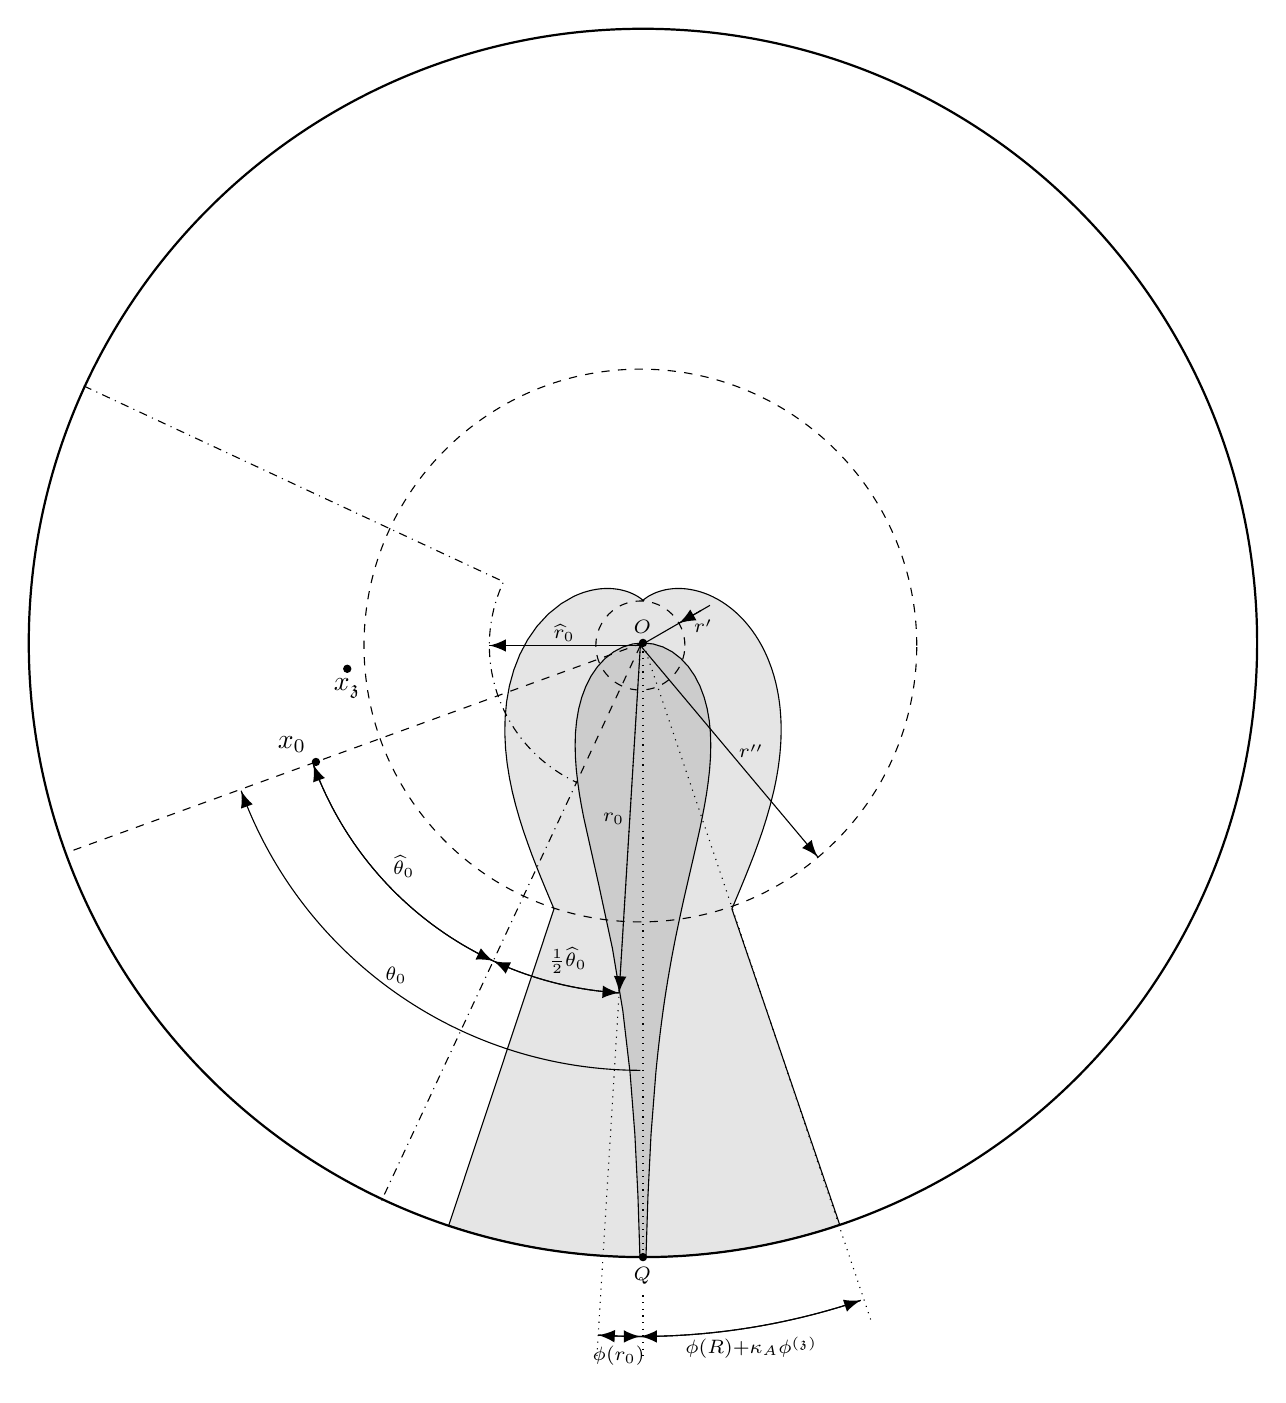
\begin{tikzpicture}[x=1cm,y=1cm,scale=0.65,
     decoration={markings,
       mark=at position 1 with {\arrow[scale=1.5,black]{latex}};
      }]
      
      \def\c{12}
      \def\barr{4}
      \def\radp{6.8}
      \def\radb{2.95}
      \def\delta{1.5}
      \def\angb{45}
      \def\phip{200}
      \def\phiro{266.5}
      \def\phiss{185}
      \def\angabs{-71.4};
      \node[inner sep=0] (O) at (\c,\c) {};
      \node[inner sep=0] (P) at (2,4) {};
      \node[inner sep=0] (Q) at (\c,0) {};
  \draw[fill=gray!20] (8.204cm,0.616cm) --(10.262cm,6.803cm) -- (10.178cm,7.003cm) -- (10.092cm,7.208cm) -- (10.005cm,7.419cm) -- (9.918cm,7.636cm) -- (9.831cm,7.859cm) -- (9.747cm,8.090cm) -- (9.664cm,8.328cm) -- (9.586cm,8.575cm) -- (9.513cm,8.830cm) -- (9.447cm,9.094cm) -- (9.391cm,9.367cm) -- (9.346cm,9.649cm) -- (9.315cm,9.940cm) -- (9.301cm,10.238cm) -- (9.307cm,10.543cm) -- (9.336cm,10.852cm) -- (9.391cm,11.162cm) -- (9.476cm,11.470cm) -- (9.593cm,11.771cm) -- (9.744cm,12.059cm) -- (9.930cm,12.326cm) -- (10.150cm,12.565cm) -- (10.402cm,12.767cm) -- (10.631cm,12.900cm) -- (10.678cm,12.923cm) -- (10.727cm,12.944cm) -- (10.775cm,12.963cm) -- (10.824cm,12.981cm) -- (10.873cm,12.997cm) -- (10.923cm,13.011cm) -- (10.972cm,13.024cm) -- (11.022cm,13.035cm) -- (11.072cm,13.044cm) -- (11.122cm,13.052cm) -- (11.172cm,13.058cm) -- (11.222cm,13.062cm) -- (11.271cm,13.064cm) -- (11.321cm,13.064cm) -- (11.370cm,13.063cm) -- (11.418cm,13.060cm) -- (11.466cm,13.054cm) -- (11.513cm,13.048cm) -- (11.560cm,13.039cm) -- (11.606cm,13.028cm) -- (11.651cm,13.016cm) -- (11.695cm,13.002cm) -- (11.738cm,12.987cm) -- (11.780cm,12.969cm) -- (11.820cm,12.950cm) -- (11.860cm,12.930cm) -- (11.898cm,12.908cm) -- (11.934cm,12.884cm) -- (11.969cm,12.859cm) -- (12.002cm,12.833cm) -- (11.998cm,12.833cm) -- (12.031cm,12.859cm) -- (12.066cm,12.884cm) -- (12.102cm,12.908cm) -- (12.140cm,12.930cm) -- (12.180cm,12.950cm) -- (12.220cm,12.969cm) -- (12.262cm,12.987cm) -- (12.305cm,13.002cm) -- (12.349cm,13.016cm) -- (12.394cm,13.028cm) -- (12.440cm,13.039cm) -- (12.487cm,13.048cm) -- (12.534cm,13.054cm) -- (12.582cm,13.060cm) -- (12.630cm,13.063cm) -- (12.679cm,13.064cm) -- (12.729cm,13.064cm) -- (12.778cm,13.062cm) -- (12.828cm,13.058cm) -- (12.878cm,13.052cm) -- (12.928cm,13.044cm) -- (12.978cm,13.035cm) -- (13.028cm,13.024cm) -- (13.077cm,13.011cm) -- (13.127cm,12.997cm) -- (13.176cm,12.981cm) -- (13.225cm,12.963cm) -- (13.273cm,12.944cm) -- (13.322cm,12.923cm) -- (13.369cm,12.900cm) -- (13.416cm,12.876cm) -- (13.463cm,12.851cm) -- (13.509cm,12.824cm) -- (13.554cm,12.796cm) -- (13.598cm,12.767cm) -- (13.642cm,12.736cm) -- (13.685cm,12.704cm) -- (13.728cm,12.671cm) -- (13.769cm,12.637cm) -- (13.810cm,12.601cm) -- (13.850cm,12.565cm) -- (13.889cm,12.527cm) -- (13.927cm,12.489cm) -- (13.964cm,12.450cm) -- (14.000cm,12.409cm) -- (14.035cm,12.368cm) -- (14.070cm,12.326cm) -- (14.103cm,12.283cm) -- (14.136cm,12.240cm) -- (14.167cm,12.195cm) -- (14.198cm,12.150cm) -- (14.227cm,12.105cm) -- (14.256cm,12.059cm) -- (14.283cm,12.012cm) -- (14.310cm,11.965cm) -- (14.336cm,11.917cm) -- (14.360cm,11.869cm) -- (14.384cm,11.820cm) -- (14.407cm,11.771cm) -- (14.429cm,11.722cm) -- (14.449cm,11.672cm) -- (14.469cm,11.622cm) -- (14.488cm,11.571cm) -- (14.507cm,11.521cm) -- (14.524cm,11.470cm) -- (14.540cm,11.419cm) -- (14.556cm,11.368cm) -- (14.570cm,11.317cm) -- (14.584cm,11.265cm) -- (14.597cm,11.214cm) -- (14.609cm,11.162cm) -- (14.620cm,11.110cm) -- (14.630cm,11.059cm) -- (14.640cm,11.007cm) -- (14.649cm,10.955cm) -- (14.657cm,10.903cm) -- (14.664cm,10.852cm) -- (14.671cm,10.800cm) -- (14.677cm,10.748cm) -- (14.682cm,10.697cm) -- (14.686cm,10.645cm) -- (14.690cm,10.594cm) -- (14.693cm,10.543cm) -- (14.696cm,10.492cm) -- (14.698cm,10.441cm) -- (14.699cm,10.390cm) -- (14.700cm,10.339cm) -- (14.700cm,10.288cm) -- (14.699cm,10.238cm) -- (14.698cm,10.188cm) -- (14.697cm,10.138cm) -- (14.695cm,10.088cm) -- (14.692cm,10.038cm) -- (14.689cm,9.989cm) -- (14.685cm,9.940cm) -- (14.681cm,9.891cm) -- (14.677cm,9.842cm) -- (14.672cm,9.793cm) -- (14.666cm,9.745cm) -- (14.661cm,9.697cm) -- (14.654cm,9.649cm) -- (14.648cm,9.601cm) -- (14.641cm,9.554cm) -- (14.634cm,9.507cm) -- (14.626cm,9.460cm) -- (14.618cm,9.413cm) -- (14.609cm,9.367cm) -- (14.601cm,9.321cm) -- (14.592cm,9.275cm) -- (14.582cm,9.229cm) -- (14.573cm,9.184cm) -- (14.553cm,9.094cm) -- (14.487cm,8.830cm) -- (14.414cm,8.575cm) -- (14.336cm,8.328cm) -- (14.253cm,8.090cm) -- (14.169cm,7.859cm) -- (14.082cm,7.636cm) -- (13.995cm,7.419cm) -- (13.908cm,7.208cm) -- (13.822cm,7.003cm) -- (13.738cm,6.803cm) -- (15.845cm,0.633cm) --(15.475cm,0.514cm) --(15.101cm,0.408cm) --(14.724cm,0.313cm) --(14.344cm,0.231cm) --(13.961cm,0.161cm) --(13.577cm,0.104cm) --(13.190cm,0.059cm) --(12.803cm,0.027cm) --(12.415cm,0.007cm) --(12.026cm,0.000cm) --(11.637cm,0.005cm) --(11.249cm,0.024cm) --(10.861cm,0.054cm) --(10.475cm,0.097cm) --(10.090cm,0.153cm) --(9.707cm,0.221cm) --(9.327cm,0.302cm) --(8.949cm,0.394cm) --(8.575cm,0.499cm) --(8.204cm,0.616cm) --cycle;

\draw[fill=gray!40] (11.941cm,0.000cm) -- (11.902cm,1.200cm) -- (11.842cm,2.401cm) -- (11.748cm,3.604cm) -- (11.607cm,4.811cm) -- (11.404cm,6.030cm) -- (11.136cm,7.278cm) -- (10.842cm,8.591cm) -- (10.798cm,8.820cm) -- (10.758cm,9.051cm) -- (10.725cm,9.285cm) -- (10.698cm,9.521cm) -- (10.681cm,9.760cm) -- (10.675cm,9.999cm) -- (10.681cm,10.239cm) -- (10.704cm,10.477cm) -- (10.744cm,10.711cm) -- (10.804cm,10.938cm) -- (10.885cm,11.154cm) -- (10.988cm,11.356cm) -- (11.113cm,11.538cm) -- (11.260cm,11.696cm) -- (11.426cm,11.825cm) -- (11.608cm,11.921cm) -- (11.801cm,11.980cm) -- (12.000cm,12.000cm) --(12.199cm,11.980cm) -- (12.392cm,11.921cm) -- (12.574cm,11.825cm) -- (12.740cm,11.696cm) -- (12.887cm,11.538cm) -- (13.012cm,11.356cm) -- (13.115cm,11.154cm) -- (13.196cm,10.938cm) -- (13.256cm,10.711cm) -- (13.296cm,10.477cm) -- (13.319cm,10.239cm) -- (13.325cm,9.999cm) -- (13.319cm,9.760cm) -- (13.302cm,9.521cm) -- (13.275cm,9.285cm) -- (13.242cm,9.051cm) -- (13.202cm,8.820cm) -- (13.158cm,8.591cm) -- (13.112cm,8.366cm) -- (13.063cm,8.144cm) -- (13.013cm,7.924cm) -- (12.963cm,7.707cm) -- (12.913cm,7.492cm) -- (12.864cm,7.278cm) -- (12.815cm,7.067cm) -- (12.768cm,6.857cm) -- (12.723cm,6.649cm) -- (12.679cm,6.441cm) -- (12.636cm,6.235cm) -- (12.596cm,6.030cm) -- (12.557cm,5.825cm) -- (12.521cm,5.621cm) -- (12.486cm,5.418cm) -- (12.453cm,5.215cm) -- (12.422cm,5.013cm) -- (12.393cm,4.811cm) -- (12.366cm,4.609cm) -- (12.340cm,4.408cm) -- (12.316cm,4.206cm) -- (12.293cm,4.005cm) -- (12.272cm,3.805cm) -- (12.252cm,3.604cm) -- (12.158cm,2.401cm) -- (12.098cm,1.200cm) -- (12.059cm,0.000cm) -- (12.059cm,0.000cm) -- (12.045cm,0.000cm) -- (12.030cm,0.000cm) -- (12.015cm,0.000cm) -- (12.000cm,0.000cm) -- (11.985cm,0.000cm) -- (11.970cm,0.000cm) -- (11.955cm,0.000cm) -- (11.941cm,0.000cm) -- cycle;
\draw[fill=black] (O) ++(\phiss:\radp-1) circle (0.07) node[right, below] {$x_{\ss}$};
\draw[fill=black] (O) ++(\phip:\radp) circle (0.07) node[above left] {$x_0$};
\draw[dashed] (O)  ++(\phip:0) -- ++(\phip:\c);

      \draw[dotted] (O) -- (Q);
      \draw[dotted] (O) -- ++(\angabs:\c+2);
      \draw[dotted] (\c,-0.75) -- (\c,-2);
      \begin{scope}[xshift=340,yshift=340]
        \draw[dash dot] (\phip-\angb:\c) -- (\phip-\angb:\radb) arc (\phip-\angb:\phip+\angb:\radb) -- (\phip+\angb:\c);
        \draw[postaction={decorate}] (\phip:\radp) arc (\phip:\phip+\angb:\radp);
        \draw[postaction={decorate}] (\phip+\angb:\radp) arc (\phip+\angb:\phip:\radp) node[midway,xshift=7.5pt,yshift=5pt] {$_{\widehat{\theta}_0}$};
        \draw[dashed] (0,0) -- (\phip+\angb:\radb);
        \draw[postaction={decorate}] (\phiro:\radp) arc (\phiro:\phip+\angb:\radp) node[midway, above, xshift=5pt] {$_{\frac12\widehat{\theta}_0}$};
        \draw[postaction={decorate}] (\phip+\angb:\radp) arc (\phip+\angb:\phiro:\radp);
        \draw[postaction={decorate}] (270:\radp+\delta) arc (270:\phip:\radp+\delta) node[midway, above] {$_{\theta_0}$};
        %\draw[postaction={decorate}] (\phip:\radp+\delta) arc (\phip:270:\radp+\delta);
        \draw[postaction={decorate}] (270:\c+1.5) arc (270:360+\angabs:\c+1.5) node[midway, below] {$_{\phi(R)+\kappa_A\phi^{(\ss)}}$};
        \draw[postaction={decorate}] (360+\angabs:\c+1.5) arc (360+\angabs:270:\c+1.5);
        \draw[postaction={decorate}] (\phiro:\c+1.5) arc (\phiro:270:\c+1.5) node[midway, below] {$_{\phi(r_0)}$};
        \draw[postaction={decorate}] (270:\c+1.5) arc (270:\phiro:\c+1.5);
     % \draw[fill=black] (\phiro:\radp) circle (0.08) node[above, xshift=5pt] {$_{B_0}$};       
        \draw[postaction={decorate}] (0,0) -- (\phiro:\radp) node[midway, left, xshift=2pt] {$_{r_0}$};
      \draw[dotted] (0,0) -- (\phiro:\c+2);
      \draw[dashed] (0,0) circle (5.4);
      \draw[postaction={decorate}] (0,0) -- (-50:5.4) node[midway, right] {$_{r''}$};
      \draw[dashed] (0,0) circle (0.87);
      \draw (0,0) -- (30:1.37);
      \draw[postaction={decorate}] (30:1.57) -- (30:0.87) node [right, xshift=2pt,yshift=-1pt] {$_{r'}$};
      \draw[postaction={decorate}] (0,0) -- (180:\radb) node [midway, above, yshift=-2pt] {$_{\widehat{r}_0}$};
      \end{scope}
      \draw[thick,black] (\c,\c) circle (\c);
      \draw[fill=black] (Q) circle (0.07);
      \draw[fill=black] (O) circle (0.07);
      \node[below] at (Q) {$_Q$};      
      \node[above] at (O) {$_O$}; 
	\end{tikzpicture}
    \caption{(a) The lightly shaded area corresponds to $\dt(\KA)\setminus B_{Q}(R)$ as defined in Theorem~\ref{thm:mixedLarge} and the strongly shaded region represents $B_Q(R)$. (b) The smallest (respectively largest) circumference whose
    boundary is a dashed line is of radius $r'$
    ($r''$, respectively). 
    (c) The region whose boundary is the dashed-dot line corresponds to the box $\mathcal{B}(x_0):=[\widehat{r}_0,R]\times [\theta_0-\widehat{\theta}_0,\theta_0+\widehat{\theta}_0]$ when $\ss$ is large.}
    \label{fig:mixto}
\end{figure}
%\cml{If the picture contains the box, then it should be placed in the upper bounds section no?}
%\cmk{Below I only refer to item (a) of the picture. In the upper bound secton I will refer to item (b), and so on until all of its aspects are introduced. Sounds ok?}\cml{ok then!}\dmc{Maybe we could have three figures: the one only with the grey area here, only part (a). Then, once the box is described, also the box (which is (a) and (c). And then finally the radii $r'$ and $r''$ which also (b)}\dmc{I thought the old version had the right $\hat{\theta}_0$ that is half of the width of the box around $x_0$}

We refer to Figure~\ref{fig:mixto}(a) for an illustration of $\dt(\KA)$ as defined in the last theorem.

\medskip
The following subsection is dedicated to proving the lower bounds of the two theorems just stated (in fact, as can be seen from the proof, the assumptions about $\ss$ are slightly milder in the proofs). The subsequent subsection then deals with the corresponding upper bounds.


\subsection{Lower bounds}\label{sec:Lower}
%
In this subsection we prove the lower bounds of Theorem~\ref{thm:mixedSmall} and~\ref{thm:mixedLarge}.

\subsubsection{The case $\ss$ small}
We start with the proof of the lower bound of Theorem~\ref{thm:mixedSmall}. 
We establish the following proposition, which proves the  lower bound of Theorem~\ref{thm:mixedSmall}. %\dmc{You are right that the bound $\ss \in \Omega(n^{4\beta-2})$ is not needed for the proof. But if $\ss$ is even smaller than the right hand side is less than constant. Should we still put it? For me ok, so I left for now your suggestion of statement}\cmk{I would remove the superflous assumption.}\dmc{Ok, took out the lower bound on $\ss=\Omega(n^{4\beta-2})$}
\begin{proposition}\label{generalschico_lower}
 Fix $\beta\le\frac{1}{2}$ and take $\dt$ as in~\eqref{mix:lower:defD}. If $\ss=O(1)$, then
\[\int_{\dt}\P_{x_0}(T_{det}\leq \ss)d\mu(x_0) 
\;=\; \Omega(ne^{-\beta R}\sqrt{\ss}).\]
\end{proposition}
\begin{proof}
Consider $x_0$ with $|\theta_0| \le \phi(r_0)+\sqrt{\ss} e^{-\beta r_0}$ and $r_0 \ge c$ for some constant $c > 0$. Note that for such choice of $r_0$ we have $\coth(r_0)\leq\coth(c)=O(1)$ and thus within time $O(1)$, with probability bounded away from zero, the radial coordinate changes by at most $1$. Conditioning on this, we consider the angular movement variance $1$ Brownian motion $B_{\II{\ss}}$ where now $\II{\ss}:=\int_0^\ss\cosech^2(\beta r_{\ss})d\ss\geq (\sqrt{\ss}/\sinh(\beta(r_0+1))^2$. As in the proof of Theorem~\ref{thm:mainangular}, define the exit time $H_{[-a,b]}$ from the interval $[-a,b]$ where
 $a:=\phi(r_0+1)-|\theta_0|$ and $b:=2\pi-\phi(r_0+1)-|\theta_0|$, and as in~\eqref{eqn:angular-exitt} in the proof of Theorem~\ref{thm:mainangular},
$$
\mathbb{P}_{x_0}(T_{det} \le \ss) \ge \mathbb{P}(H_{[-a,b]} \le \II{\ss})=\Omega\big(\Phi\big((\phi(r_0+1)-|\theta_0|)\sinh(\beta (r_0+1))/\sqrt{\ss}\big)\big).
$$
Since $\phi(\cdot)>0$ and $\sinh(x)\leq e^{x}$ we conclude that $\PP_{x_0}(T_{det}\le \ss)
  =\Omega(\Phi(-|\theta_0|e^{\beta (r_0+1)}/\sqrt{\ss}))$.
Integrating over the elements of $\dt$ satisfying $|\theta_0| \le \sqrt{\ss} e^{-\beta r_0}$, 
%\dmc{here I can afford on purpose not to put $\phi(r_0)$,} 
we have
$$
\int_{\dt} \mathbb{P}_{x_0}(T_{det} \le \ss) d\mu(x_0) =
\Omega(ne^{-\alpha R})\int_{1}^R \int_0^{\sqrt{\ss} e^{-\beta \widehat{r}_0}} 
\Phi(-\theta_0 e^{\beta \widehat{r}_0}/\sqrt{\ss})\sinh(\alpha \widehat{r}_0) d\theta_0 d\widehat{r}_0. 
$$
Performing the change of variables $y_0:=\theta_0 e^{\beta \widehat{r}_0}/\sqrt{\ss}$, since $\alpha>\beta$, and using $\sinh(x)=\Theta(e^x)$ for $x=\Omega(1)$, we get for the latter
$$
\Omega(ne^{-\alpha R})\int_0^{1} \Phi(-y_0)\sqrt{\ss}dy_0\int_{1}^R e^{(\alpha-\beta)\widehat{r}_0} d\widehat{r}_0=\Omega(ne^{-\beta R}\sqrt{\ss})\int_0^{1} \Phi(-y_0) dy_0.
$$
Note that the last integral is $\Omega(1)$, and thus the stated result follows.
%\cmk{Where is the hypothesis $\ss=\Omega(n^{4\beta-2})$ used?}\dmc{It is not needed in the proof, but I put it for the statement: if $\ss$ is right of this order, the conclusion gives a constant right hand size. If $\ss$ is even smaller  }
\end{proof}


\subsubsection{The case $\ss$ large}
We now prove the lower bound of Theorem~\ref{thm:mixedLarge}. In fact, we will only need to assume the milder condition $\ss \ge Ce^{2\KA^2}$ with $C$ being a large enough constant. %\cmk{Is this phrase really needed here? Why?}\dmc{Ok now?}. 
We start by showing that particles that start close to the origin detect quickly with at least constant probability:
\begin{lemma}\label{lem:closetoorigin}
Let $\tau > 0$, and let $c^*:=C^*/\beta$ for some arbitrarily large constant $C^* > 0$. Then,
$$
 \inf_{x_0\in B_O(c^*)}\PP_{x_0}(T_{det}\leq \tau)=\Omega(1).
$$
\end{lemma}
\begin{proof}
Let $T_{h}$ be the smallest time $t$ such that $r_t=2c^*$ and notice that, calling $\PP^r$ the law of the radial component of the process, for any point $x_0=(r_0, \theta_0)$ with~$r_0 \le c^*$, it holds that
$\PP^r_{r_0}(T_{h}\ge \tau)\,\geq\,\PP^r_{c^*}(T_{h} \ge \tau).$
Now, fix any realization $\{r_s\}_{s\geq 0}$ of the radial component of the process such that~$T_h\ge\tau $ and observe that for any such realization, detection is guaranteed if $|\theta_s-\theta_0|>2\pi$ for some $0 \le s \le \tau$. Under the event $T_{h}\ge\tau$ the radial coordinate at any time $s \le \tau$ is at most $2c^*$. Thus, the angular movement $\theta_\tau-\theta_0$ has a normal distribution centered at zero with variance at least
\[\int_0^{\tau}\sinh^{-2}(\beta r_s)ds\,\geq\, \tau\sinh^{-2}(2C^*)  =\Omega(1).\]
Thus, with constant probability, within time~$\tau$ the angular movement covers an angle of $2\pi$. The lemma follows. 
\end{proof}
%We may and will thus in the following always assume that $r_0 > c^*$ for $c^*$ as in the statement of Lemma~\ref{lem:closetoorigin}. 


We now deal with the remaining starting points $x_0\in\dt$.
Before doing so we establish a simple fact concerning the random variables defined for nonnegative integer values of $k$ as follows:
\begin{equation}\label{mixedLower:def:Ik}
I_k := \int_0^\ss {\bf 1}_{(0,k]}(r_s)ds.
\end{equation}
Recall that $\pi(r):=\frac{\alpha\sinh(\alpha r)}{\cosh(\alpha R)-1}$, $0\leq r\leq R$, is the stationary distribution of the process~$\{r_s\}_{s\geq 0}$.
\begin{fact}\label{fact:stationary}
If $k\geq\frac{1}{\alpha}\log 2$, 
then $\EE_{\pi}(I_k) \ge \tfrac14\ss e^{-\alpha (R-k)}$.
\end{fact}
\begin{proof}
Suppose $r_0$  is distributed according to the stationary distribution $\pi$. 
Since $\cosh(x)-1\leq \frac12 e^x$, by definition of $I_k$, we have
\[
\EE_{\pi}(I_k) = \int_0^{\ss}\PP_{\pi}(r_s\leq k)ds =\ss\pi((0,k]) = \ss\cdot\frac{\cosh(\alpha k)-1}{\cosh(\alpha R)-1}
\geq 2\ss e^{-\alpha R}(\cosh(\alpha k)-1).
\]
The desired conclusion follows observing that the map $x\mapsto 1+e^{-2x}-2e^{-x}$ is non-decreasing, and thus for $x\geq\log 2$, we have 
$\cosh(x)-1=\frac12 e^x(1+e^{-2x}-2e^{-x})\geq\frac14 e^{x}$.
\end{proof}

We are now ready to state and prove the proposition dealing with particles whose initial position are points satisfying the first condition in the definition of $\dt$:
\begin{proposition}\label{mixedLowerBoundschico}
Let $\KA > 1$. There is a sufficiently large constant $C>0$ such that if $\ss\ge Ce^{2\KA^2}$ and $\ss=O(\mathfrak{Z})$, then for any $x_0=(r_0, \theta_0)$ with $|\theta_0| \le \phi(R)+\KA \phis$, we have the following: 
\begin{enumerate}[(i)]

\item\label{mixedLowerBoundschico:imt1}  If $\alpha \ge 2\beta$, then $\displaystyle 
\PP_{x_0}(T_{det} \leq \ss)=\Omega(\tfrac{1}{\KA}e^{-\frac12\KA^2}) =\Omega(e^{-0.7\KA^2})$. %\cmk{I don't understand, what issue?}\dmc{I mean we don't have matching upper and lower bounds, let's ignore this. Ok, I commented out the asymptotics with respect to $\KR$ and put $\KA$ only. Also merged cases (ii) and (iii) from before according to your suggestion} 

\item\label{mixedLowerBoundschico:imt2} 
%If $\alpha < 2\beta$ and $\beta \ge 1/2$, then \dmc{I think when merging conditions, I forgot to update here. It should be just: "If $\alpha < 2\beta$ then $\PP_{x_0}(T_{det} \leq \ss) = \Omega(\KA^{-(2 \wedge \frac{1}{\beta})\alpha})$, right? we could also separate cases as in Proposition 32. Or merge them therein, as you wish. But it should be consistent}
If $\alpha < 2\beta$, then %\dmc{It was $\wedge$ before, but it should be $\vee. $, I changed it. Check} 
$\displaystyle
\PP_{x_0}(T_{det} \leq \ss) = \Omega(\KA^{-\alpha/(\beta\wedge\frac12)})$.
%$\displaystyle
%\PP_{x_0}(T_{det} \leq \ss) = %\Omega(\KA^{-2\alpha}).%=\Omega(\KR^{-2\alpha}).
%$
\end{enumerate}
\end{proposition}
To prove the just stated proposition we use the following standard fact several times, so we state it explicitly.
%\dmc{I say it is standard, but important: $\eta > 0$ is a uniform bound. It is Feller's lemma 7.1, commented still in the preliminaries. I think we need only $\kappa > 1$ (strictly bigger than $1$) to have this uniform bound.}\cmk{As far as I can tell, I think the bound is correct for $\kappa\geq 1$ even taking $\eta=\frac32$ provided you are willing to accept a multiplicative $\frac{1}{\sqrt{2\pi}}$ factor. Check www.johndcook.com/blog/norm-dist-bounds/}\dmc{We can put the exact lower bound given in your link of $1/(\sqrt{2\pi}) \frac{t}{t^2+1}e^{-t^2/2}$ for $\P(X > t)$. So where is $3/2$ in the exponent? In any case, it is not matching upper bounds...}\cmk{Just use that $1+t^2\leq e^{t^2}$ and you get a lowe bound of $\frac{t}{\sqrt{2\pi}e^{-\frac32 t^2}}$. You may them either assume $t\geq \sqrt{2\pi}$ and use the lower bound $e^{-\frac32 t^2}$ or use $t\geq 1$ and use the lower bound $\frac{1}{\sqrt{2\pi}}e^{-\frac32 t^2}$.}\dmc{Ok, adapted it below}
\begin{fact}[\cite{gordon41}]\label{mixedLower:fact:brownian}
Given the radial component $\{r_{s}\}_{s\geq 0}$ of a particle's trajectory,  the angular component $\{\theta_s\}_{s\geq 0}$ law is that of a Brownian motion indexed by $\II{\ss}:=\int_0^{\ss}\cosech^2(\beta r_s)ds$. 
If $\II{\ss} \ge \sigma^2 > 0$ and $\kappa>0$, then 
%\dmc{(should we just cite www.johndcook.com/blog/norm-dist-bounds/ ?}\cmk{Let me first try to find a more standard reference.}
\[
\PP(\sup_{0\leq s\leq \ss} B_{\II{s}}\geq \kappa \sigma \mid \{r_s\}_{s\geq 0}) \geq  \frac{\kappa}{\sqrt{2\pi}(\kappa^2+1)}e^{-\frac12\kappa^2}=\Omega\Big(\frac{1}{\kappa}e^{-\frac12\kappa^2}\Big).
\]
\end{fact}
Now we proceed with the pending proof.
\begin{proof}[Proof of Proposition~\ref{mixedLowerBoundschico}.]
Assume first $\beta \ge 1/2$
(and thus necessarily $\alpha < 2\beta$). In this case the radial movement dominates and the proof of~\eqref{mixedLowerBoundschico:imt2} is very similar to the one given for $x_0 \in \dt$ where $|\theta_0|\le \phi(R)+\kappa\phis$: assume first that $\ss$ (and $\KA$) is such that $|\theta_0|\le \phi(R)+\KA \phis \le \pi/2 - c$ for some $c > 0$. Define $\overline{r}_0$ be as $\rabs_0$ in the proof of Proposition~\ref{prop:rad-upperBnd} (that is $\overline{r}_0$ corresponds to the absorption radius in case there was radial movement only; since $\phi(R)+\KA \phis \le \pi/2 - c$, we have $\overline{r}_0=\Omega(1)$). By the same argument as given in the proof of Proposition~\ref{prop:rad-upperBnd}, with $\KA$ playing the role of $\kappa$ therein, with probability $\Omega(\KA^{-2\alpha})$, there exists a time moment $T \le \ss$, at which a radial value of $\overline{r}_0$ is reached. In this case, by symmetry of the angular movement, with probability at least $1/2$, either the angle at time $T$ satisfies $|\theta_T| \le |\theta_0|$ or there exists $t \le T$ where the angle $\theta_t=0$ and we detected already by time $t$, and hence in this case $Q$ is detected by time $T$ with probability $\Omega(\KA^{-2\alpha})$. Assume then that~$\ss$ (and $\KA$) is such that $\pi/2 - c \le \phi(R)+\KA \phis$. In this case, let $\overline{r}_0$ be equal  (assuming there were radial movement only) to the absorption radius $\rabs_0$ that would correspond to an angle exactly $|\theta_0|=\pi/2 -c$. Note that in this case $\overline{r}_0=\Theta(1)$. By the proof of Proposition~\ref{prop:rad-upperBnd}, with probability $\Omega(\KA^{-2\alpha})$ a radial value of $\overline{r}_0$ is reached at a time moment  $T \le \frac12\ss$. In this case, with probability at least $1/2$, as before, either there existed a moment $t$ with $\theta_t=0$, and we would have detected $Q$, or $|\theta_T|\le|\theta_0|$. In this case, by Lemma~\ref{lem:closetoorigin}, since $\overline{r}_0=\Theta(1)$, with constant probability we detect $Q$ in time $\frac12\ss=\Omega(1)$, and hence also in this case $Q$ is detected by time $\ss$ with probability $\Omega(\KA^{-2\alpha})$.


Consider thus $x_0 \in \dt$ with $|\theta_0| \le \phi(R)+\KA\phi^{(\ss)}$ under the assumption $\beta < 1/2$. Recall that we also may assume that $r_0 \ge c^*$ for $c^*$ as in the statement of Lemma~\ref{lem:closetoorigin} since other values of $r_0$ were already dealt with in said lemma.
First, note that for $x_0 \in B_Q(R)$ the lower bound trivially holds. 
So, henceforth let $x_0 \in \dt \setminus B_Q(R)$. Since by hypothesis $\ss\in O(\mathfrak{Z})=O(e^{\alpha R})$, we may assume that $\ss < \exp(\alpha(R-\frac{1}{\alpha}\log 2 - 1+c))$ for $c>0$ sufficiently large. %By hypothesis, taking $C$ sufficiently large, \dm{with room to spare}, we may also assume that $\ss \ge e^{\alpha c}$.
Let $\rho:=R-\frac{1}{\alpha}\log\ss+c$ and note that $\frac{1}{\alpha}\log 2+1 < \rho$ by the previous assumption on $\ss$. 
%\cmk{Also, you did not answer my question regarding where do we use the upper bound on $\rho$.}\dmc{I think you're right about this, I removed it. We use  below only that $g(\overline{\rho} $ is always bounded away from $R$, so I think no need for this, indeed}.
%\dmc{Changes from here on, since change in the strategy}  
Denote by $T_{\rho-1}$ the random variable corresponding to the first time the process reaches $B_O(\rho-1)$. Recall from Part~\eqref{radial:itm:phi2} of Lemma~\ref{lemmaradial}, with $\yabs_0=\rho-1$ and $\auxY=R$, that for the radial component $\{r_s\}_{s\geq 0}$ of the movement, and for any $r_0 \in [\rho-1, R]$,
	\[\EE_{r_0}(T_{\rho-1})\leq\frac{4}{\alpha^2}e^{\alpha(R-\rho+1)}
	=\frac{4}{\alpha^2} \ss e^{-\alpha(c-1)}.
	\]
	By Markov's inequality, for $c$ sufficiently large so that  $\frac{4}{\alpha^2}e^{-\alpha(c-1)} \le \frac14$, it follows that the event $\mathcal{A}$ corresponding to the process reaching $B_O(\rho-1)$ 
	before time $\frac12\ss$ happens with
	probability
	\[\PP(\mathcal{A})=1-\PP_{r_0}(T_{\rho-1}\geq \tfrac12 \ss) \ge \tfrac{1}{2}.\]
	Now, let $\overline{\rho}:=\max\{\rho-\beta \log \KA, c^*\}.$ Moreover, define $\mathcal{B}$ as the event that starting from radius $\rho-1$ we hit the radial value $\overline{\rho}$ before hitting the radial value $R$.
	Define $g(r):=\log(\tanh(\frac12\alpha R)/\tanh(\frac12\alpha r))$ as in Fact~\ref{fct:radial-varphi2} and observe that as argued therein,
	since $\rho=\Omega(1)$ we have $g(\rho-1)=O(e^{-\alpha \rho})$ and because
	$\overline{\rho}=R-\Omega(1)$ we have $g(\overline{\rho})=\Omega(e^{-\alpha \overline{\rho}})$. Recall from Part~\eqref{radial:itm:phi3} of Lemma~\ref{lemmaradial} that $g(\rho-1)/g(\overline{\rho})$ is the probability that starting from radius $\rho-1$ we hit the radial value $\overline{\rho}$ before hitting the radial value $R$, and we have
$$
\PP(\mathcal{B})=\frac{g(\rho-1)}{g(\overline{\rho})}=\Omega(e^{\alpha(\overline{\rho}-\rho)})=
%e^{\alpha(\max\{\rho-\frac{1}{\beta}\log \KA, c^*\}-\rho)}=
\Omega(\KA^{-\alpha/\beta}).%=\Omega(\KR^{-\alpha/\beta}).
$$
 From Part~\eqref{radial:itm:phi4} of Lemma~\ref{lemmaradial} we obtain 
$$
\EE_{\rho-1}(T_{\overline{\rho}} \mid T_{\overline{\rho}} < T_R) \le \frac{2}{\alpha}(\beta \log \KA+1)+\frac{2}{\alpha^2} \le \frac{\ss}{8},
$$
where the last inequality follows (with room to spare) by our assumption of $\ss$.
Thus, by Markov's inequality, conditionally under $\mathcal A \cap \mathcal B$,
%\cmk{Well, my point is that event $\mathcal{A}$ ocurring tells us we have reached $\rho-1$, it does not say we have reached $\rho$.}\dmc{Good catch, I adapted it}
with probability at least $\frac12$, we reach $\overline{\rho}$ before time $\frac34\ss$. Let $\mathcal C$ be the corresponding event. Conditional under $\mathcal C$, with constant probability the particle stays one unit of time inside $B_O(\overline{\rho}+1)$ before time $\ss$, and let this event be called $\mathcal D$. Conditional under $\mathcal D$, the angular component's law during one unit of time inside $B_O(\overline{\rho}+1)$ is $B_{\II{\ss}}$ with $$\II{\ss}\ge \cosech^2(\beta(\overline{\rho}+1)) \ge e^{-2\beta(\overline{\rho}+1)} \geq e^{-2\beta (R-\frac{1}{\alpha}\log\ss+c-\frac{1}{\beta}\log \KA +1)}=:\sigma^2.$$
Note that $\sigma = e^{-\beta R}\ss^{\frac{\beta}{\alpha}}\KA e^{-\beta(c+1)}$ for the absolute constant $c > 0$ independent of $\KA$ from above, and recall also that
 $|\theta_0| \le \phi(R)+\KA \ss^{\frac{\beta}{\alpha}}e^{-\beta R} \le 2\KA \ss^{\frac{\beta}{\alpha}}e^{-\beta R}$ by assumptions on $\beta < 1/2$ and $\ss$, with room to spare. 
Let $\mathcal{E}$ be the event that when reaching $B_O(\overline{\rho}+1)$ the angle at the origin spanned by the particle and $Q$ is (in absolute value) is at most $|\theta_0|$ or there was a moment $t$ before reaching $B_O(\overline{\rho}+1)$ with $\theta_t=0$ (and thus we detected at time $t$). Note that by symmetry of the angular movement, $\PP(\mathcal{E})\ge \frac12$.
 Conditional under $\mathcal{D} \cap \mathcal{E}$, by Fact~\ref{mixedLower:fact:brownian},  since $\KA > 1$, for some $c_1=c_1(c)$ we have
\[
\P_{x_0}(T_{det}\leq\ss)\geq \PP(\sup_{0\leq s\leq \ss} B_{\II{s}}\geq c_1 \sigma \mid \{r_s\}_{s\geq 0}) =\Omega(1),
\]
 and since $\mathcal{D} \cap \mathcal{E}$ holds with probability $\Omega(\KA^{-\alpha/\beta})$, we have
 $
\P_{x_0}(T_{det}\leq\ss)= \Omega(\KA^{-\alpha/\beta})$,
which finishes the proof of the case $\alpha < 2\beta$ and $\beta < 1/2$ (and thus the proof of~\eqref{mixedLowerBoundschico:imt2}).


 We now deal with the remaining $\alpha \ge 2\beta$ case (and therefore necessarily $\beta < 1/2$). Assume first $\alpha > 2\beta$. This argument is analogous to the one for angular movement: we repeat it for convenience. 
%Since $|\theta_0|\le \kappa e^{-\beta R}\sqrt{\ss}+\phi(r_0)$, 
Given the trajectory of $\{r_{s}\}_{s\geq 0}$, recall that the angular component's law is that of a Brownian motion $B_{\II{\ss}}$, where $\II{\ss}:=\int_0^{\ss} \cosech^2(\beta r_s)ds \ge 4\ss e^{-2\beta R} =: \sigma^2$.
Hence, using Fact~\ref{mixedLower:fact:brownian}, since $\KA > 1$ and using that $0.2x^2\ge \log x$ for all $x\ge 1$,
%\[
%\PP(\sup_{0\leq s\leq \ss} B_{\II{s}}\geq \KA \sigma \mid \{r_s\}_{s\geq 0}) \geq  %e^{-\eta \KA^2},
%\]
%and so
$$
\P_{x_0}(T_{det}\leq\ss)\geq \PP(\sup_{0\leq s\leq \ss} B_{\II{s}}\geq \KA \sigma \mid \{r_s\}_{s\geq 0}) =\Omega\big(-\tfrac{1}{\KA}e^{-\frac12\KA^2}\big)={\Omega(e^{-0.7\KA^2})}, 
$$
showing the result in the case $\alpha > 2\beta$.


Finally, suppose $\alpha=2\beta$ (therefore $\beta > \frac14$).
First, suppose that the starting point $r_0$ of the radial component is distributed according to the stationary distribution of the process, that is, $\pi(r):=\frac{\alpha\sinh(\alpha r)}{\cosh(\alpha R)-1}$ with $0\leq r\leq R$. 
%\dmc{At the end of the proof I remove this assumption, it was missing before}
We will see that the contribution to  $\II{\ss}:=\int_0^{\ss} \cosech^2(\beta r_s) ds$ of the time spent around different radial values is roughly the same, forcing a logarithmic correction. To bound $\II{\ss}$ from below, let $\overline{k}=R-\lfloor\tfrac{1}{\alpha}\log (\ss/4) \rfloor$, which by our hypothesis $\ss= O(\mathfrak{Z})=O(e^{\alpha R}/(\alpha R))$ implies $\overline{k}=\omega(1)$ (in particular it implies also $\overline{k} \ge \frac{1}{\alpha}\log 2$). 
Note that 
\[
\II{\ss} = \int_0^{\overline{k}}\cosech^2(\beta r_s)ds
  + \!\sum_{k=\overline{k}+1}^R \int_{k-1}^{k}\cosech^2(\beta r_s)ds
      \geq 4\Big(I_{\overline{k}}e^{-2\beta \overline{k}}+\!\sum_{k=\overline{k}+1}^R (I_k - I_{k-1})e^{-2\beta k}\Big).
\]
Hence, using that $\beta\geq\frac14$ implies that $4(1-e^{-2\beta})\geq 1$,
\begin{equation}%\label{eqn:hlowbound}
    \II{\ss} 
    \geq 4\Big(\sum_{k=\overline{k}}^{R-1}I_ke^{-2\beta k}(1-e^{-2\beta}) +I_R e^{-2\beta R} \Big)
    \ge \sum_{k=\overline{k}}^R e^{-2\beta k}I_{k}.
\end{equation}
 So, recalling that $\overline{k}\ge \frac{1}{\alpha}\log 2$, by Fact~\ref{fact:stationary}, for all $k \in \{\overline{k},\ldots,R\}$, we have $\EE_{\pi}(I_k)\geq \frac14 \ss e^{-\alpha(R-k)}$,
which gives an estimate for the value of the $I_k$ variables. Moreover, by Corollary~\ref{radial:cor:coupling}, %\cmk{This $C$ is related to the $C$ in the statement of Propostion 31, but it is not used/mentioned in what follows. The $C$ plays a role in the necessary hypothesis for applying Proposition 31, that is, $\ss\geq Ce^{\alpha(\auxY-k)}$. In fact, shouldn't we justify why this condition is satisfied?}\dmc{Indeed. I try. I don't want to put the $C$ of the proposition, just the $\widetilde{C}$, this is enough, I think. In that proposition the $C$ there in the statement is redundant I think, need to check again, but plan to remove it} 
since $k \ge \overline{k}$ and by definition of $\overline{k}$ we have $\ss \ge 4e^{\alpha (R-\overline{k})} \ge 4e^{\alpha (R-k)}$. Since $\cosh(x)-1=\frac12 e^x(1-e^{-x})^2\le \frac12 e^x$, using once more that $k\ge\overline{k}\ge\frac{1}{\alpha}\log 2$, we obtain %\dmc{if you agree above it is $e^{-\alpha(R-k)}(1-e^{-\alpha k})^2$, and $\frac14$ is enough instead of $\frac{1}{12}$, I think} 
$\pi((0,k])\ge e^{-\alpha(R-k)}(1-e^{-\frac12\alpha k})^2\ge \frac{1}{4}e^{-\alpha(R-k)}$, so $\ss\ge 1/\pi((0,k])$ and the assumptions of Corollary~\ref{radial:cor:coupling} are satisfied. Hence, there exist $\widetilde{c}, \widetilde{\eta} \in (0,1)$, such that for each $\overline{k} \le k \le R$, we have that the expectation of the indicator $Z_k$ of the event $\{I_k\geq \widetilde{c}\ss e^{-\alpha (R-k)}\}$ is at least~$\widetilde{\eta}$. Let $Z:=\sum_{k=\overline{k}}^R Z_k$ and that $\EE(Z) \ge (R-\overline{k}+1)\widetilde{\eta}$. Define then the event 
$\mathcal{E}:=\{Z>\frac{\widetilde{\eta}}{2}(R-\overline{k}+1)\}$. Since $\EE(Z)\le (\PP(\mathcal{E})+\frac{\widetilde{\eta}}{2}\PP(\overline{\mathcal{E}}))(R-\overline{k}+1)$,
it must be the case that $\PP(\mathcal{E})\ge\frac{\widetilde{\eta}}{2}/(1-\frac{\widetilde{\eta}}{2})\ge\frac{\widetilde{\eta}}{2}$.
Thus, for a fixed realization of $\{r_s\}_{s\geq 0}$ satisfying $\mathcal{E}$, since $\alpha=2\beta$, we have 
\[
%\frac{1}{4(1-e^{-2\beta})}\II{\ss}
\sum_{k=\overline{k}}^{R}e^{-2\beta k}I_k 
\geq\sum_{k=\overline{k}}^{R}e^{-2\beta k}\widetilde{c}\ss e^{-\alpha (R-k)}Z_k
= \widetilde{c}\ss e^{-2\beta R}\sum_{k=\overline{k}}^R Z_k 
> \widetilde{c}\ss e^{-2\beta R}\frac{\widetilde{\eta}}{2}(R-\overline{k}+1).
\]
Note that  $R-\overline{k}+1\ge \frac{1}{\alpha}\log (\ss/4)$ by definition of $\overline{k}$, so 
$
\sum_{k=\overline{k}}^R e^{-2\beta k}I_k\geq \frac{\widetilde{c}}{2\alpha}\widetilde{\eta}\ss e^{-2\beta R}\log(\ss/4)) \ge \frac{\widetilde{c}}{3\alpha}\widetilde{\eta}\ss e^{-2\beta R}\log\ss,
$
where we used the assumption that $\ss$ is at least a sufficiently large constant.
Thus, under $\mathcal{E}$ the angular movement dominates stochastically
a Brownian motion $B_{\frac{\widetilde{c}}{3\alpha}\widetilde{\eta}\ss e^{-2\beta R}\log\ss}$ with standard deviation 
$e^{-\beta R}\sqrt{(\widetilde{c}\ss \widetilde{\eta}/(3\alpha))\log\ss}=:\sigma$. By Fact~\ref{mixedLower:fact:brownian}, %\dmc{Should we put $3/2$ instead of $c$?} 
\[
\PP(\sup_{0\leq s\leq \ss} B_{\II{s}}\geq \KA \sigma \mid \{r_s\}_{s\geq 0})=\Omega(\tfrac{1}{\KA}e^{-\frac12\KA^2}).
\]
Thus, for $x_0 \in \dt$ with $|\theta_0| \le \phi(R)+\KA \phis\le 2\KA e^{-\beta R}\sqrt{\ss \log \ss}$, since $\P_{x_0}(\mathcal{E})\geq \frac{\widetilde{\eta}}{2}$ and using that $0.2x^2\ge \log x$ for all $x\ge 1$,
\begin{equation}\label{startstationary}
\P_{x_0}(T_{det}\le \ss)\geq \tfrac{\widetilde{\eta}}{2}\P_{x_0}(T_{det} \le \ss \mid \mathcal{E})=\Omega(\tfrac{1}{\KA}e^{-\frac12\KA^2})=\Omega(e^{-0.7\KA^2}).%\dm{=\KR^{-c}}.%\Omega(\Phi(-\kappa)).
\end{equation}

It remains to show thus that with positive probability the trajectory starting with a fixed initial radius for $x_0 \in \dt$ can be coupled in such a way that the probability of detection of the target by time $\ss$ can be bounded from below by the probability of detection when the radius is chosen according to the stationary distribution $\pi(\cdot)$. Denote by $\widehat{r}_t$ the radial component at time $t$ when starting according to the stationary distribution.
Consider the event $\mathcal{A}$ that the initial radial value $\widehat{r}_0$ is at most one unit away from the 
boundary of $B_O(R)$, that is, $\mathcal{A}:=\{\widehat{r}_0\in [R-1,R]\}$.
Clearly, $\PP(\mathcal{A})=\pi([R-1,R])=\Omega(1)$. 
Let $\mathcal{B}$ be the event that $\{\widehat{r}_s\}_{s\geq 0}$ starting from $R-1$ hits $R$ by time $\frac12\ss$. 
Conditional under $\mathcal{A}$, since the time to hit $R$ is clearly dominated by the time a standard  Brownian motion (corresponding to a one-dimensional radial movement) hits $R$ starting from $R-1$, by our lower bound on $\ss$, we have that $\PP(\mathcal{B}\mid \mathcal{A})=\Omega(1)$.  Note that conditional under $\mathcal{A}\cap\mathcal{B}$ either the trajectories starting with a fixed value of $r_0$ on the one hand and with $\widehat{r}_0$ according to the stationary distribution $\pi(\cdot)$ on the other hand must cross by time $\frac12\ss$ (and they can be coupled naturally from then on for a time interval of $\frac12\ss$), or $r_t \le \widehat{r}_t$ for any $0 \le t \le \frac12\ss$, and during an initial time period of length $\frac12\ss$ the detection probability starting from $r_0$ stochastically dominates the one when starting from $\widehat{r}_0$. Thus, with probability $\PP(\mathcal{A}\cap\mathcal{B})=\Omega(1)$, the process $\{r_s\}_{s\geq 0}$ can be successfully coupled with $\{\widehat{r}_s\}_{s\geq 0}$, and since we aim for a lower bound, we assume that $\mathcal{A}\cap\mathcal{B}$ holds. Conditional under $\mathcal{A}\cap\mathcal{B}$, we may thus apply the reasoning yielding~\eqref{startstationary} with $\ss$ replaced by $\frac12\ss$, and the result follows.
%For the second bound, note that by definition of $\dt$, the set of $x_0$ with $|\theta_0| \le \kappa \phis\added[id=mk]{+\phi(r_0)}$ is contained in $\dt$ (which is a sector of $B_O(R)$, and the corollary follows by combining Proposition~\ref{uniformlowerbound} together with angular symmetry of the distribution of the particles.
\end{proof}



%\dmc{This was originally before, now it is after the first condition}
We still have to deal with particles whose initial location are points satisfying the second condition in the definition of $\dt$. The next proposition does this.
\begin{proposition}\label{prop:uniformlowerboundN2}
Let $\KR >1$ and assume that $\ss\ge Ce^{2\KA^2}$ for $C$ large enough.
%\dmc{This assumption is enough for all cases, but not needed in some, of course}. 
Then, for any $x_0=(r_0,\theta_0)$ with 
$(|\theta_0|-\phi(r_0))e^{(\beta\wedge\frac12)r_0} \le \KR$, we have the following: 
%\[\PP_{x_0}(T_{det}\leq \ss)= \Omega(\KR^{- (\alpha/\beta \wedge  2\alpha)})\]
\begin{enumerate}[(i)]

\item\label{prop:uniformLowerboundN2:itm1} If $\alpha \ge 2\beta$, then 
$\displaystyle 
\PP_{x_0}(T_{det} \leq \ss)=\Omega(\KR^{-\frac{\alpha}{\beta}})
=\Omega(e^{-{\frac{\alpha}{\beta}\KA^2}}).
$
\item\label{prop:uniformLowerboundN2:itm2} If $\alpha < 2\beta$, % and $\beta \ge 1/2$,
then  
$\displaystyle
\PP_{x_0}(T_{det} \leq \ss) = \Omega(\KR^{-\alpha/(\beta\wedge\frac12)})=\Omega(\KA^{-\alpha/(\beta\wedge\frac12)}).
$
%\item\label{prop:uniformLowerboundN2:itm3} If $\alpha < 2 \beta$ and $\beta < 1/2$, then 
%$\displaystyle
%\PP_{x_0}(T_{det} \leq \ss) =\Omega(\KR^{-\alpha/\beta})=\Omega(\KA^{-\alpha/\beta}).
%$
\end{enumerate}
\end{proposition}
\begin{proof}
Thanks to Lemma~\ref{lem:closetoorigin} we may, and will, assume throughout the proof that
$r_0>c^*$ for an arbitrarily large $c^*$. Under said condition, the proof argument formalizes the following intuitive fact: Either there is a chance for the particle to move radially towards the origin so that the boundary of $B_Q(R)$ is reached and detection happens, or there is a chance to move radially towards the origin, enough so that the particle stays long enough in such a region close enough to the origin so that the relatively large angle the particle traverses makes detection probable.

We first assume $\beta<1/2$.
%address the proof of~\eqref{prop:uniformLowerboundN2:itm1} and~\eqref{prop:uniformLowerboundN2:itm3} together. Note that $\alpha \ge 2\beta$ implies $\beta < 1/2$, and so in both cases we have $\beta < 1/2$.  
Observe that we may assume $|\theta_0|\ge 2\phi(r_0)$, since otherwise during one time unit there is constant probability that the radial value is at most $\min\{R,r_0+1\}$, and conditional under this event, during this time unit with constant probability an angular movement of standard deviation at least $e^{-\beta (r_0+1)}$ is performed, thus covering with constant probability an angular distance of $e^{-\beta(r_0+1)} \ge 2\phi(r_0)$ in the case of $\beta < 1/2$ for $r_0 > c^*$. We may and will thus below replace the condition $(|\theta_0|-\phi(r_0))e^{(\beta\wedge\frac12)r_0} \le \KR$ by $|\theta_0|e^{(\beta\wedge\frac12)r_0} \le 2\KR$. We consider the worst-case scenario, i.e., $|\theta_0|=2\KR e^{-\beta r_0}$, or equivalently $r_0=\frac{1}{\beta}\log(2\KR/|\theta_0|)$. %\dmc{I think contrary to  Prop 26, here this special treatment is needed sinc we go for a lower bound $g(r_0)/g(\overline{r}_0)$ below} 
We restrict our discussion to vertices with $r_0 < R-\log \KA$, as other vertices were already considered before: indeed, for values of $r_0 \ge R-\log \KA$, in case~\eqref{prop:uniformLowerboundN2:itm1}
we have $2\KR e^{-\beta r_0} = 2e^{\KA^2}e^{-\beta r_0} \le e^{\KA^2}e^{-\beta R}\KA \le \KA \sqrt{\ss}e^{-\beta R}=\KA \phis$, where the second inequality follows from our assumption of $\ss\ge Ce^{2\KA^2}$ with $C$ large. Hence such values of $x_0=(\theta_0, r_0)$ satisfy the first condition of $\dt$ and were treated in Proposition~\ref{mixedLowerBoundschico}. In case~\eqref{prop:uniformLowerboundN2:itm2}, for values of $r_0 \ge R-\log \KA$, we have $2\KR e^{-\beta r_0}=2\KA e^{-\beta r_0}\le 2\KA^2 e^{-\beta R}\le \KA \phis$, where again the second inequality follows from the same assumption on $\ss \ge Ce^{2\KA^2}$ (again with room to spare), and again this case was already dealt with in Proposition~\ref{mixedLowerBoundschico}.
Define $g(r):=\log(\tanh(\frac12 \alpha R)/\tanh(\frac12 \alpha r))$ as in Fact~\ref{fct:radial-varphi2} and let $\overline{r}_0:=\max\{r_0-\frac{1}{\beta}\log \KR, c^*\}$. By arguments given in said fact, since we have restricted our discussion to the case where $r_0=R-\Omega(1)$, we have $g(r_0)=\Omega(e^{-\alpha r_0})$ and, since $\overline{r}_0\geq c^*$ with $c^*$ large, we also have $g(\overline{r}_0)=O(e^{-\alpha \overline{r}_0})$. %\dmc{Please check that the preceding is ok - I hope so. if not, I have to change a bit the preceding paragraph and exclude other values of $r_0$ already}
Recall from Part~\eqref{radial:itm:phi3} of Lemma~\ref{lemmaradial} that $g(r_0)/g(\overline{r}_0)$ is the probability that starting from radius $r_0$ we hit the radial value $\overline{r}_0$ before hitting the radial value $R$, and we have
$$
\frac{g(r_0)}{g(\overline{r}_0)}=\Omega(e^{\alpha(\overline{r}_0-r_0)})=
\Omega(e^{\alpha(\max\{r_0-\frac{1}{\beta}\log \KR, c^*\}-r_0)})=\Omega(\KR^{-\alpha/\beta}).
%=\Omega(e^{-\dm{\eta}\KA^2})
$$
Thus, by Part~\eqref{radial:itm:phi4} of Lemma~\ref{lemmaradial} with $\auxy_0:=\overline{r}_0$ and $\auxY:=R$, we have that $\EE_{r_0} (T_{\overline{r}_0} \mid T_{\overline{r}_0} < T_R) \le \frac{2}{\alpha\beta}\log \KR + \frac{2}{\alpha^2} \le \frac14\ss$ by our lower bound hypothesis of $\ss$ with $C:=C(\beta)$ sufficiently large. 
%\dmc{For now $C$ depends on $\beta$, if we don't want this, we have to put $\beta \ge \varepsilon' > 0$ as assumption.}
By Markov's inequality,  conditional under $T_{\overline{r}_0} < T_R$, starting at radius $r_0$, with probability at least $1/2$, the value of $\overline{r}_0$ is hit by time $\frac12\ss$. In this case, if $\overline{r}_0=c^*$, then by Lemma~\ref{lem:closetoorigin} the target is detected with constant probability in constant time, and we are done. If $\overline{r}_0 =r_0-\frac{1}{\beta}\log \KR > c^*$, then with constant probability, during the ensuing unit time interval, the radial coordinate $r$ is always at most $\overline{r}_0+1$. Call this event $\mathcal{A}$. By symmetry of the angular movement, with probability at least $1/2$, either the angle $\theta$ at the hitting time of~$\overline{r}_0$ is in absolute value at most $|\theta_0|$ or there was a time moment $t$ with $\theta_t=0$ before, and we had detected $Q$ by time $t$ already. Call this event~$\mathcal{B}$. Conditional under $\mathcal{A} \cap \mathcal{B}$, the variance of the angular movement after reaching $\overline{r}_0$ during the following unit time interval is at least 
$
e^{-2\beta (r_0-\frac{1}{\beta}\log\KR+1)} =e^{-2\beta (r_0+1)}\KR^2$,
so recalling that by our worst-case assumption $|\theta_0|=2\KR e^{-\beta r_0}$,  the standard deviation is thus at least $e^{-\beta (r_0+1)}\KR=e^{-\beta}|\theta_0|/2$. Hence, with constant probability, independently of $\KR$ (and also independently of $\beta$), in this case an angle of $|\theta_0|$ is covered during a unit time interval, and by our lower bound assumption of $\ss$, the particle is detected by time $\ss$, finishing also this case and %both the proof 
%of Part~\eqref{prop:uniformLowerboundN2:itm1} and Part~\eqref{prop:uniformLowerboundN2:itm3} 
establishing the proposition when $\beta<1/2$ 
by plugging in the respective relations between $\KA$ and $\KR$ in order to obtain the last equality of the the two parts of the statement.

Next, we consider Part~\eqref{prop:uniformLowerboundN2:itm2} which encompasses a case similar to the one analyzed in Section~\ref{sec:radial}, so we give only a short sketch of how it is handled. By hypothesis and case assumption $|\theta_0| \le \phi(r_0)+\KR e^{-\frac12r_0}$. Since $\KR >1$, we thus have $|\theta_0|\le 3\KR e^{-\frac12r_0}$. Again, it suffices to show the statement for the worst-case scenario, that is, we may assume $|\theta_0|= 3\KR e^{-\frac12r_0}$. We may assume that $r_0 < R- \KR$, since for vertices with $r_0 \ge R-\KR$, using our assumption of $\ss\ge Ce^{2\KA^2}$ (with room to spare) we have
$3\KR e^{-\frac12r_0} \le 3\KR e^{\KR} e^{-\frac12 R} \le \KA \ss^{1/(2\alpha) e^{-\frac12 R}}=\KA \phis$, and such cases were already dealt with in the proof of Part~\eqref{mixedLowerBoundschico:imt2}  of Proposition~\ref{mixedLowerBoundschico}. By Lemma~\ref{lem:closetoorigin} we may also assume $r_0 > c^*$ for arbitrarily large $c^*$.
Define $\overline{r}_0:=\max\{r_0-2 \log \KR-2, c^{*}\}$. 
As before, recall from Part~\eqref{radial:itm:phi3} of Lemma~\ref{lemmaradial} that $g(r_0)/g(\overline{r}_0)$ is the probability that starting from radius $r_0$ we hit the radial value $\overline{r}_0$ before hitting the radial value $R$. Since $r_0=R-\Omega(1)$ and since $\overline{r}_0 \ge c^*$, we have
$$
\frac{g(r_0)}{g(\overline{r}_0)}=\Omega(e^{\alpha(\overline{r}_0-r_0)})=
\Omega(e^{\alpha(\max\{r_0-2\log \KR-2, c^*\}-r_0)})=\Omega(\KR^{-2\alpha}),
%=\Omega(e^{-\dm{\eta}\KA^2})
$$
and let $\mathcal{A}$ be the event that this indeed happens. 
By Part~\eqref{radial:itm:phi4} of Lemma~\ref{lemmaradial} with $\auxy_0:=\overline{r}_0$ and $\auxY:=R$, we have that $\EE_{x_0}(T_{\overline{r}_0}\mid \mathcal{A}) \le \frac{4}{\alpha}\log \KR +\frac{4}{\alpha}+ \frac{2}{\alpha^2} \le \frac14\ss$ by our lower bound hypothesis on $\ss$. By Markov's inequality, with probability at least $1/2$, $T_{\overline{r}_0} < \frac12\ss$. Let $\mathcal{B}$ be the event to reach the radius $\overline{r}_0$ by time $\frac12\ss$.
We have
$$
\PP_{x_0}(\mathcal{B}) \ge \PP_{x_0}(\mathcal{B} \mid \mathcal{A})\PP_{x_0}(\mathcal{A}) =\Omega(\KR^{-2\alpha}).
$$

 Let $\mathcal{C}$ be the event that one of the following events occurs: Either at the moment $T$ when reaching $\overline{r}_0$ the angle made at the origin between the particle and $Q$ is in absolute value at most $|\theta_0|$, or there was a moment $t \le T$ where $\theta_t=0$ (and we already detected $Q$ by time $t$). Note that by symmetry of the angular movement, $\PP_{x_0}(\mathcal{C} \mid \mathcal{B})=\PP_{x_0}(\mathcal{C}) \ge 1/2$. Hence, $\PP_{x_0}(\mathcal{C} \cap \mathcal{B})=\Omega(\KR^{-2\alpha})$. To conclude observe first the following:
 If it is the case that $\overline{r}_0=c^*$, then conditional under $\mathcal{C} \cap \mathcal{B}$, by Lemma~\ref{lem:closetoorigin}, with constant probability, in time $O(1)$ the particle $Q$ is detected, and since $\frac12\ss+O(1) \le \ss$, we are done. In particular, if 
we had $|\theta_0| > \pi/2 - c$ for some sufficiently small $c > 0$, then, since $|\theta_0| \le 3\KR e^{-\beta r_0}$, we must have $r_0 < c^*$, and therefore clearly also $\overline{r}_0=c^*$. If on the other hand we had  $|\theta_0| \le \pi/2 - c$ for some arbitrarily small $c > 0$ and also $\overline{r}_0=r_0-2\log \KR$, then observe that since $\overline{r}_0 > c^*$ with $c^*$ large enough, we have
$\phi(\overline{r}_0) \ge e 1.99\KR e^{-r_0/2} \ge 3\KR e^{-r_0/2} \ge |\theta_0|$, and $Q$ is detected by time $T$, since $\phi(\overline{r}_0)$ corresponds to the maximum angle at the origin between a particle at radius $\overline{r}_0$ and $Q$ that guarantees detection. 
\end{proof}

The uniform lower bound of Theorem~\ref{thm:mixedLarge} now follows directly by combining Proposition~\ref{mixedLowerBoundschico} and Proposition~\ref{prop:uniformlowerboundN2}. The integral lower bound of Theorem~\ref{thm:mixedLarge} follows directly from Proposition~\ref{mixedLowerBoundschico} applied with $\KA$ being any fixed constant and the fact that $\mu(\dt)=\Omega(n\phis)$ (by considering the condition $|\theta_0| \le \phi(R)+\KA \phis$ only), and the proofs of the lower bounds of Theorem~\ref{thm:mixedSmall} and Theorem~\ref{thm:mixedLarge} are finished. %\dmc{Marcos, I would leave out the remaining from here on}
%We conclude the section stating the following corollary which shows that the contribution of the measure of $\dt$ that comes from points satisfying the first condition in the definition of $\dt$ is asymptotically already of the same order as the matching upper bound shown below in Section~\ref{sec:Upper}, \dm{as we claimed in Theorem~\ref{thm:mixed}.}
%\begin{corollary}\label{cor:schico}Fix $\beta>0$, $\KA > 1$, and take $\dt$ as in~\eqref{mix:eqn:defDs}. There is a sufficiently large $C>0$ such that if $\ss \ge C e^{2\KA^2}$ %\dmc{This assumption is enough for all cases, but not needed in some, of course} satisfies the conditions of Theorem~\ref{thm:intro-mixed}, then 
%\[\int_{\dt}\P_{x_0}(T_{det}\leq \ss)d\mu(x_0) \;=\; \Omega(e^{-\frac12R}\phis).\]
%\end{corollary}
%\cmk{Shouldn't we remove the $\KA$'s from the corollary above? We are goint to fix the all $\kappa$'s in the integral bounds, right? Also, shouldn't we state somewhere what the value of $\mu(\dt)$ is (similarly to what was done in previous sections)?}

\subsection{Upper bounds}\label{sec:Upper}

In this section we will show the corresponding upper bounds of Theorems~\ref{thm:mixedSmall} and~\ref{thm:mixedLarge}: that is, we show that particles initially placed outside $\dt$, with $\dt$ as in the corresponding theorems, have only a small chance of detecting the target by time $\ss$. For all values of $\ss$, we will show that
\[\int_{\ndt}\PP_{x_0}(T_{det}\leq \ss)d\mu(x_0)=O(\mu(\dt)),\]
thus establishing that the significant contribution %\dmc{either add: "for $\KA$ large enough" or replace by "a significant contribution"} 
to the tail probabilities comes from particles inside $\dt$, and for large values of $\ss$ we will show uniform upper bounds for the detection probability of every point outside $\dt$. %\cmk{I find very odd to say that "particles" have strategies. This notion is something that we came up to talk about how a particle that has significant chance of detecting behaves. Either we need to explain clearly what we mean by strategy or stop using it.}\cml{I think that the intuition of particles having optimal strategies for detection is interesting so maybe it could be good to discuss it somewhere. I will delete all mentions of strategies for now} 
In order to analyze the trajectory of a particle we will make use of the fact that the generator driving its motion can be separated into its radial and angular component, given respectively by
\[\Delta_{rad} = \frac{1}{2}\frac{\partial^2}{\partial r^2}+\frac{\alpha}{2}\frac{1}{\tanh(\alpha r)}\frac{\partial}{\partial r}\quad\text{and}\quad \Delta_{ang}=\frac{1}{2\sinh^2(\beta r)}\frac{\partial^2}{\partial\theta^2}.\]
Since the generator driving the radial part of the motion does not depend on $\theta$, our approach consists in sampling the radial component $\{r_s\}_{s\geq0}$ of the trajectories first and then, conditional under a given radial trajectory, sampling the angular component $\{\theta_s\}_{s\geq0}$. With this approach we can make use of the results obtained in Section~\ref{sec:radial} in order to study $\{r_s\}_{s\geq 0}$, while the angular component is distributed according to a time-changed Brownian motion $\theta_s=B_{\II{s}}$, where
%\cmk{Double check that in the lower bound section we got rid of the $h(\cdot)$'s and replaced them by $I(\cdot)$.}\dmc{I can see it still in Section 3 in the proof of the main theorem there. Equation (12) and before, it should be changed there, right?}\cmk{Yes!}\cml{If solved, please remove}
\[\II{s}:=\int_0^s\cosech^{2}(\beta r_u)du\]
relates the radial trajectory to the angular variance of $\{\theta_s\}_{s\geq 0}$, as already seen in Section~\ref{sec:angular}. To be able to apply the insight obtained by studying each component separately, we will need to replace the hitting time of the target (which translates into hitting $B_Q(R)$ whose boundary defines a curve relating $r$ and $\theta$) by the exit time of a simpler set: let $x_0\in\ndt$ be any fixed initial location with $\theta_0\in(0,\pi)$  and define a box $\mathcal{B}(x_0)$ containing~$x_0$, of the form 
\begin{equation}\label{eqn:up:box}
\mathcal{B}(x_0):=[\hatr,R]\times[\theta_0-\hatt,\theta_0+\hatt]\subseteq \overline{B}_Q(R)
\end{equation}
where $\hatt$ and $\hatr$ will be defined later on. %\cmk{Can't both consitions be satisfied, how is $\ss$ defined then?}\dmc{At this point we could just say depending on whether $\ss$ is small or large}\cml{when $\ss=\Theta(1)$ the definitions are of the same order (and we could use either proof to obtain the bounds). How would you write this fact? Maybe just not mention it now and say that $\hatt$ and $\hatr$ will be defined later?}
Since $\mathcal{B}(x_0)\subseteq\overline{B}_Q(R)$, it follows that in order for a particle starting at $x_0$ to detect the target, it must first exit the box through either its upper boundary or its side boundaries. Denoting by $\trad$ and $\tang$ the respective hitting times of said boundaries, this implies that $\trad\wedge \tang\leq T_{det}$, and we can obtain the bound
\begin{equation}\label{boxboundsNew}\PP_{x_0}(T_{det}\leq \ss)\,\leq\,\PP_{x_0}(\trad\leq \ss)+\PP_{x_0}(\tang\leq \ss<\trad).\end{equation}
The advantage of addressing the exit time of $\mathcal{B}(x_0)$ instead of $T_{det}$ is straightforward; the first event $\{T_0^{rad}\le \ss\}$ is independent of the angular component of the trajectory, allowing us to bound from above its probability with the tools developed in Section~\ref{sec:radial}, while the treatment of the second event $\{T_0^{ang}\le \ss<T_0^{rad}\}$ will follow from standard results on Brownian motion and the control of~$\II{\ss}$. The following result allows us to bound the second term on the right-hand side of~\eqref{boxboundsNew}:
\begin{proposition}\label{prop:mainuppermixed}
Define $J(r):=\cosech^{-2}(\beta r)$. Then,
\[\PP_{x_0}(\tang\leq \ss\leq\trad)\,\leq\,4\Phi\Big({-}\frac{\hatt}{\sqrt{\ss\JJ(\hatr)}}\Big).\]
where $\Phi$ stands for the error function. Furthermore, %\deleted[id=al]{if $\frac18\hatt^2\in[\ss\JJ(R),\ss]$, then}
\[\PP_{x_0}(\tang\leq \ss)\leq \sqrt{\frac{2}{\pi}}\int_{0}^{\infty}\frac{\hatt}{\sigma^{3/2}}e^{-\frac{\hatt^2}{2\sigma}}\PP_{x_0}\big(\II{\ss}\geq\sigma\big)d\sigma.
\]
%\cml{Notice that there is a big change for this term, will have to redo more than a few computations}\dmc{Agree with the new result. Left the colors in the proof below for Marcos}
\end{proposition}
\begin{proof}
Denote by $\PP_{x_0}(\cdot\mid\{r_u\}_{u\geq0})$ the law of the angular process given a realization of its radial component. Given such a realization we already know that the trajectory $\{\theta_u\}_{u\geq0}$ is equal in law to that of the time-changed Brownian motion $\{B_{\II{u}}+\theta_0\}_{u\geq0}$, for which $\tang$ is equal to the exit time of $B_{\II{u}}$ from $[-\hatt,\hatt]$. Since the exit time of a Brownian motion is well known, we proceed as in Section~\ref{sec:angular} using the reflection principle to obtain 
\[\PP_{x_0}(\tang\leq \ss\,|\{r_u\}_{u\geq0})\leq 4\PP_{x_0}(B_{\II{\ss}}\leq -\hatt\mid\{r_u\}_{u\geq 0})=4\Phi\Big({-}\frac{\hatt}{\sqrt{\II{\ss}}}\Big)\]
where the factor 4 is obtained since the probability of exiting by hitting one of the angles is twice the probability of hitting any of the two angles, which is twice the probability of hitting one fixed angle. Taking expectations with respect to the law of $\{r_u\}_{u\geq 0}$ we obtain
\[\PP_{x_0}(\tang\leq \ss\leq\trad)\leq 4\EE_{x_0}\Big(\Phi\Big({-}\frac{\hatt}{\sqrt{\II{\ss}}}\Big){\bf 1}_{\{\ss\leq\trad\}}\Big),\]
where the expression within the expectation depends on the radial movement alone. To apply this last bound observe that for any realization of $\{r_u\}_{u\geq0}$ such that $\trad\geq\ss$ we have that $\inf_{0\leq u\leq\ss}r_u\geq \hatr$, so $\II{\ss}\leq \ss\JJ(\hatr)$, which gives the first part of the proposition's statement. For the second part of the proposition we can make the same computation as before without taking into account the event $\{\trad\geq\ss\}$, giving 
\[\PP_{x_0}(\tang\leq \ss)\,\leq\,4\EE_{x_0}\Big(\Phi\Big({-}\frac{\hatt}{\sqrt{\II{\ss}}}\Big)\Big)\,=\,-4\int_{0}^\infty\Phi\Big({-}\frac{\hatt}{\sqrt{\sigma}}\Big)d\PP_{x_0}\big(\II{\ss}\geq\sigma\big),\]
and the result follows after using integration by parts, since $\frac{d}{d\sigma}\Phi(-\frac{\hatt}{\sqrt{\sigma}})=\frac{1}{2\sqrt{2\pi}}\frac{\hatt}{\sigma^{3/2}}e^{-\frac{\hatt^2}{2\sigma}}$.
 \end{proof}
 
 \smallskip
 
On a high level, in the proposition above, the bound for $\PP_{x_0}(\tang\leq \ss<\trad)$ will be useful as long as $\ss=O(1)$ since in this case the inequality $\ss \JJ(\hatr)\leq \II{\ss}$ is not too loose. However, when $\ss=\omega(1)$ we need to control this term using the second part of Proposition~\ref{prop:mainuppermixed}, which relies heavily on bounding probabilities of the form $\PP(\II{\ss}\geq\sigma)$. To provide these bounds observe that when $\inf_{0\leq u\leq\ss}r_u$ is not too close to zero the drift function is almost constant so the trajectories of $\{r_u\}_{u\geq0}$ resemble those of a Brownian motion with drift $\tfrac{\alpha}{2}$ (with a reflecting boundary at $R$). Even further, on the event where $\inf_{0\leq u\leq\ss}r_u$ is not too close to zero we also have
\begin{equation}\label{eq:approximation}\II{\ss}\approx\int_0^\ss e^{-2\beta r_u}du,\end{equation}
where  %and we also have that the drift is almost constant and the trajectories of $\{r_u\}_{u\geq0}$ resemble those of a Brownian motion with constant drift $\tfrac{\alpha}{2}$ (with a reflecting boundary at $R$),  and we can also perform the following approximation
%\begin{equation}\label{eq:approximation}\II{\ss}\approx\int_0^\ss e^{-2\beta r_u}du.\end{equation}
%The behavior of random variables such as
the integral appearing above on the right-hand side has been widely studied in the case when $\{r_u\}_{u\geq 0}$ is an (unbounded) Brownian motion with drift (see~\cite{matsumoto2005,Yor1992,Feng2020,dufresne}), revealing that their distributions are heavy-tailed with the tail exponent given analytically in terms of $\beta$ and the drift of $\{r_u\}_{u\geq 0}$. In order to make use of known results  we must first address the change in behavior arising from the reflecting boundary of our process. To do so, we consider an auxiliary process $\{\widetilde{r}_u\}_{u\geq 0}$ akin to the one introduced in the proof of Proposition~\ref{prop:rad-upperBnd}:
    \begin{itemize}
	\item $\{\widetilde{r}_u\}_{u\geq 0}$ begins at $r_0$ and evolves according to $\Delta_{rad}$ up until hitting $R$.
	\item Every time $\{\widetilde{r}_u\}_{u\geq 0}$ hits $R$, it is immediately restarted at $R-1$ and continues to evolve as before.
\end{itemize}
It is not hard to see that $\{\widetilde{r}_u\}_{u\geq 0}$
 is stochastically dominated by $\{r_u\}_{u\geq 0}$, in the sense that the radius of the auxiliary process is always smaller. Thus, in particular, $\II{\ss}\leq \tII{\ss} := \int_0^s\cosech^{2}(\beta \widetilde{r}_u)du$, and hence it will be enough to bound probabilities of the form $\PP(\tII{\ss}\geq\sigma)$ from above. Now, from the definition of $\widetilde{r}_u$, it is natural to use the subsequent hitting times of $R$, say $0<T_R^{(1)}<T_R^{(2)}<\ldots$, to divide the trajectory of $\{\widetilde{r}_u\}_{u\geq 0}$ into excursions from $R-1$ to $R$ (or from $r_0$ to $R$, in the case of the first one), giving
\[\tII{\ss}\,\leq\,\int_0^{T^{(1)}_R}\cosech^{2}(\beta\widetilde{r}_u)du\,+\,\sum_{i=1}^{M(\ss)}\int_{T^{(i)}_R}^{T^{(i+1)}_R}\cosech^{2}(\beta\widetilde{r}_u)du,\]
where $M(\ss)$ is a random variable equal to the amount of times $\{\widetilde{r}_u\}_{u\geq 0}$ has hit $R$ by time~$\ss$. Let $\{\widetilde{r}^{(0)}_u\}_{u\geq0},\{\widetilde{r}^{(1)}_u\}_{u\geq0},\{\widetilde{r}^{(2)}_u\}_{u\geq0},\ldots$ be independent random diffusion processes (that will correspond to the different excursions), each evolving on $(0,\infty)$ according to the generator $\Delta_{rad}$ without the reflecting boundary at $R$, and such that $\{\widetilde{r}^{(0)}_u\}_{u\geq0}$ starts at $r_0$ while the rest of the $\{\widetilde{r}^{(i)}_u\}_{u\geq0}$ start at $R-1$. From the definition of the auxiliary process it follows that within each time interval of the form $[T^{(i)}_R,T^{(i+1)}_R]$ (or $[0,T^{(1)}_R]$ in the case of the first excursion) the trajectory of $\{\widetilde{r}_u\}_{u\geq0}$ is equal to the one of $\{\widetilde{r}^{(i)}_{u'}\}_{u'\geq0}$ for $u'\leq T^{(i+1)}_R-T^{(i)}_R$. Hence,%\dmc{Why separate at the right hand side the term for $i=0$? Aha, perhaps below }\cml{it is not necessary at this point, now all the terms are in the same sum}
\[\tII{\ss}\,\leq\,\int_0^{T^{(1)}_R}\cosech^{2}(\beta\widetilde{r}^{(0)}_u)du\,+\,\sum_{i=1}^{M(\ss)}\int_{0}^{T^{(i+1)}_R-T^{(i)}_R}\cosech^{2}(\beta\widetilde{r}^{(i)}_u)du\,\leq\,\sum_{i=0}^{M(\ss)}\tI^{(i)},\]
where for $i=0, \ldots, M(\ss)$
\[\tI^{(i)}:=\int_{0}^{\infty}\cosech^{2}(\beta\widetilde{r}^{(i)}_u)du.\]
Observe that the bound on $\tII{\ss}$ involves a sum of $M(\ss)+1$ random variables. Intuitively speaking the number of times the process hits $R$ should be proportional to $\ss$, so we introduce an auxiliary parameter $v_0>0$ depending on $x_0$, to be fixed later, so that the event $M(\ss)>\lceil v_0\ss\rceil$ occurs with a very small probability. Using this new parameter we obtain
\begin{equation}\label{eq:division}\PP_{x_0}(\II{\ss}\geq\sigma)\,\leq\,\PP_{x_0}\big(M(\ss)>\lceil v_0\ss\rceil \big)+\PP_{x_0}\big(\tI^{(0)}\geq\tfrac12\sigma\big)+ \PP_{x_0}\Big(\sum_{i=1}^{\lceil v_0\ss\rceil}\tI^{(i)}\geq\tfrac12\sigma\Big).\end{equation}
The advantage of the bound above is that it involves the sum of independent random variables~$\tI^{(i)}$ which, aside from $\tI^{(0)}$, are also identically distributed. The bound also gives valuable intuition regarding the detection of the target: roughly speaking, in order for detection to take place either $x_0$ must be sufficiently close to the origin so that the angular variance coming from $\tI^{(0)}$ becomes significant, or $\ss$ must be large enough so that many excursions starting near the boundary occur, allowing for the contribution $\sum_{i=1}^{M(\ss)}\tI^{(i)}$ to be large enough. As mentioned above (the discussion following~\eqref{eq:approximation}), the distributions of the $\tI^{(i)}$ variables are heavy-tailed. In order to control their sum we make use of the following lemma, whose proof mimics closely what was done in \cite{Omelchenko2019}: since our result is slightly more precise than the one in~\cite{Omelchenko2019}, we provide it in the appendix for the sake of completeness. 

\begin{lemma}\label{lem:cotapower}
Let $S_m:=\sum_{i=1}^m Z_i$ where $\{Z_i\}_{i\in\NN}$  is a sequence of i.i.d.~absolutely continuous random variables taking values in $[1,\infty)$ such that there are $V,\gamma>0$ for which for all $x\geq 0$
\[1-F_{Z_i}(x)=\PP(Z_i\geq x)\leq Vx^{-\gamma}.\]
Then, there are $\auxc,\auxl>0$ depending on $V$, $\gamma$ and $\EE(Z_1)$  (if it exists) alone such that:
\begin{itemize}
    \item If $\gamma<1$ and $L>\auxl$, then
    $\displaystyle\PP(S_m\geq Lm^{\frac{1}{\gamma}})\leq \auxc L^{-\gamma}$.
    \item If $\gamma=1$ and $L>\auxl$, then $\displaystyle\PP(S_m\geq Lm\log(m))\leq \Big(\frac{\auxc}{L\log(m)}\Big)^{1-\frac{\auxl}{L}}$.
    \item If $\gamma>1$ and  $L>\auxl$, then
    $\displaystyle\PP(S_m\geq Lm)\,\leq\,\auxc L^{-\gamma}m^{-((\gamma-1)\wedge\frac{\gamma}{2})}$.
\end{itemize}
\end{lemma}
We can now prove the following result, which will allow us to control $\PP_{x_0}(\II{\ss}\ge\sigma)$:
\begin{proposition}\label{prop:merged-varianza}
For any $0<c<1$ there are $\auxc',\auxl'$ large depending on $\alpha$ and $\beta$ alone, such that for any $\ss\geq c$, $v_0>\frac{4}{c}$, and $x_0\in B_O(R)$ with $r_0>1$, defining $\sigma_0$ as
\[
\sigma_0 := \begin{cases}
\auxl'e^{-2\beta R}(v_0\ss)^{1\vee\frac{2\beta}{\alpha}}, &
\text{if $\alpha \neq 2\beta$,} \\
\auxl'e^{-2\beta R}v_0\ss\log(v_0\ss), &
\text{if $\alpha=2\beta$,}
\end{cases}
\]
the following statements hold for all $\sigma>\sigma_0$ and all $R$ sufficiently large:
\begin{enumerate}[(i)]
\item\label{prop:merged-varianza:itm1} $\PP_{x_0}(M(\ss)>\lceil v_0\ss\rceil )\leq e^{-\frac{1}{16} v_0^2\ss}$,
\item\label{prop:merged-varianza:itm2} $\PP_{x_0}(\tI^{(0)}\geq\tfrac12\sigma)\leq \frac{\log(\tanh(\alpha r_0/2))}{\log(\tanh(\alpha/2))}+\auxc'\sigma^{-\frac{\alpha}{2\beta}} e^{-\alpha r_0}$, and 
\item\label{prop:merged-varianza:itm3} $\PP_{x_0}\big(\sum_{i=1}^{\lceil v_0\ss\rceil}\tI^{(i)}\geq\tfrac12\sigma\big)\leq 2v_0\ss\frac{\log(\tanh(\alpha ((R-1)/2))}{\log(\tanh(\alpha/2))}+\big(\auxc'(v_0\ss)^{1\vee\frac{\alpha}{4\beta}}\sigma^{-\frac{\alpha}{2\beta}}e^{-\alpha R}\big)^{1-\mathfrak{e}}$
where
\[\mathfrak{e}:=\begin{cases}
0, &\mbox{ if }\alpha\neq 2\beta, \\[3pt]\frac{1}{\sigma e^{2\beta R}}\auxl'v_0\ss\log(v_0\ss), &\mbox{ if }\alpha=2\beta.
\end{cases}\]
\end{enumerate}
\end{proposition}
\begin{proof}
We begin with the upper bound for the term $\PP_{x_0}(M(\ss)>\lceil v_0\ss\rceil)$. By definition, the event $\{M(\ss)>  \lceil v_0\ss \rceil\}$ is equal to $\{T^{(\lceil v_0\ss\rceil)}_R\leq\ss\}$. Writing $T^{(\lceil v_0\ss\rceil)}_R=T^{(1)}_R+\sum_{i=2}^{\lceil v_0\ss\rceil}(T^{(i)}_R-T^{(i-1)}_R)$,  by Markov's inequality, for any $\lambda>0$ we deduce
\[\PP_{x_0}\big(M(\ss)>\lceil v_0\ss\rceil\big)\,\leq\,\PP_{x_0}\Big(\sum_{i=2}^{\lceil v_0\ss\rceil}(T^{(i)}_R-T^{(i-1)}_R)\leq\ss\Big)\,\leq\,e^{\lambda \ss}\EE_{x_0}\Big(\exp\big({-}\lambda\sum_{i=2}^{\lceil v_0\ss\rceil}(T^{(i)}_R-T^{(i-1)}_R)\big)\Big)\]
where the differences $T^{(i)}_R-T^{(i-1)}_R$ are i.i.d.~random variables which indicate the time it takes for excursion $\widetilde{r}^{(i-1)}$ starting at $R-1$ to reach $R$. Since each $\{\widetilde{r}^{(i)}_u\}_{u\geq 0}$ is stochastically bounded from below by a Brownian motion with constant drift $\tfrac{\alpha}{2}$, we can use Formula 2.0.1 in~\cite{Borodin2002} to obtain
\[\PP_{x_0}\big(M(\ss)>\lceil v_0\ss\rceil\big)\,\leq\,e^{\lambda \ss}\EE\big(e^{-\lambda(T^{(2)}_R-T^{(1)}_R)}\big)^{\lceil v_0\ss\rceil-1}\,\leq\,e^{\lambda \ss}\big( e^{\frac{\alpha}{2}-\sqrt{\frac{\alpha^2}{4}+2\lambda}}\big)^{\lceil v_0\ss\rceil-1}.\]
The exponent $\lambda\ss+(\lceil v_0\ss\rceil-1)(\frac{\alpha}{2}-\sqrt{\frac{\alpha^2}{4}+2\lambda})$ appearing in the last term is minimized as a function of $\lambda$ when $\ss\sqrt{\tfrac{\alpha^2}{4}+2\lambda}=\lceil v_0\ss\rceil-1$, which defines a positive $\lambda$ since $v_0\ss>4$ and $\alpha,c<1$, giving an expression for the exponent of the right-hand side of the form %\dmc{now it seems ok}
\[-\frac{1}{2\ss}(\lceil v_0\ss\rceil-1)^2-\frac{1}{8}\alpha^2\ss+\frac{1}{2}\alpha(\lceil v_0\ss\rceil-1)\leq\frac12(\lceil v_0\ss\rceil-1)\Big(\alpha-\frac{1}{\ss}(\lceil v_0\ss\rceil-1)\Big)\,\leq\,-\frac{1}{16}\,v_0^2\ss\]
where in the last inequality we used that $\lceil v_0\ss\rceil-1\geq \frac12v_0\ss$ and that $\alpha-\frac12v_0\leq -\frac14 v_0$. This proves the bound in~\eqref{prop:merged-varianza:itm1}. In order to control the probabilities appearing in~\eqref{prop:merged-varianza:itm2} and~\eqref{prop:merged-varianza:itm3} it is convenient from the point of view of computations to work under the assumption that the $\widetilde{r}^{(i)}$ processes never get too close to $0$. To do so observe that by our assumption of $r_0>1$, all the $\widetilde{r}^{(i)}$ start in $(1,\infty)$, and denote by $\tau^{(i)}_1$ the hitting time of radius $1$ by $\widetilde{r}^{(i)}$. Observe that \[\PP_{x_0}(\tI^{(0)}\geq\tfrac12\sigma)\,\leq\,\PP_{x_0}(\tau_{1}^{(0)}<\infty)+\PP_{x_0}(\tI^{(0)}\geq\tfrac12\sigma, \tau^{(0)}_{1}=\infty).\]
Using Part~\eqref{radial:itm:phi3} from Lemma~\ref{lemmaradial}, with $\yabs_0:=1$ and $\auxY:=R$,  we obtain 
\[\PP_{x_0}(\tau_{1}^{(0)}<\infty)=\lim_{R \to \infty}\PP_{x_0}(\tau_{1}^{(0)}<T_R)=\frac{\log(\tanh(\alpha r_0/2))}{\log(\tanh(\alpha/2))},\]
which gives the first term of the bound for $R$ (and thus $n$) sufficiently large. For the second term, observe that on the event $\tau^{(0)}_1=\infty$ we have $\widetilde{r}^{(0)}_u>1$ for all $u\geq0$ so there is some constant $C$ depending on $\beta$ alone such that for all $u\geq 0$, we have $\cosech^2(\beta \widetilde{r}^{(0)}_u)\leq Ce^{-2\beta \widetilde{r}^{(0)}_u}$ and hence
\[\PP_{x_0}(\tI^{(0)}\geq\tfrac12\sigma,\tau^{(0)}_{1}=\infty)\,\leq\,\PP_{x_0}\Big(C\int_0^{\infty}e^{-2\beta\widetilde{r}^{(0)}_u}du\geq\tfrac12\sigma\Big).\]
Now, notice that $\{\widetilde{r}_u^{(0)}-r_0\}_{u\geq0}$ %\dmc{Ok with brackets, but $r_0$ is always larger, right? so I would put $\{r_0-\widetilde{r}_u^{(0)}\}_{u\geq0}$}%\cml{$r_0$ is not the process $r$, but the initial condition, we subtract to get a brownian motion} 
is stochastically bounded from below by $X_u$, a Brownian motion with constant drift $\tfrac{\alpha}{2}$ so we can bound the integral within the last term from above by $\int_0^{\infty}e^{-2\beta(X_u+r_0)}du$. This particular functional of Brownian motion was studied in~\cite[Proposition~4.4.4]{dufresne}, where it was shown that
\[\int_0^\infty e^{-2\beta X_u}du\,=\,W,\quad\text{where }W\text{ is a positive r.v.~with }\quad f_{W}(x):=\frac{(2\beta^2)^\frac{\alpha}{2\beta}}{\Gamma(\frac{\alpha}{2\beta})}x^{-\frac{\alpha}{2\beta}-1}e^{-\frac{2\beta^2}{x}}\]
that is, $W$ is distributed according to an inverse gamma distribution with parameters $\frac{\alpha}{2\beta}$ and~$2\beta^2$. From the density of the variable $W$ above the only relevant feature for our purposes is its heavy tail: in order to ease calculations we will bound $W$ stochastically from above by a random variable $Z$ following a Pareto distribution with a sufficiently large scale $\omega$ depending on $\alpha$ and $\beta$ alone (in particular we will assume $\omega>1$), and shape $\frac{\alpha}{2\beta}$. That is, $W \preccurlyeq Z$ with
\[f_{Z}(x)\,=\,\frac{2\beta}{\alpha\omega}\Big(\frac{\omega}{x}\Big)^{\frac{\alpha}{2\beta}+1}{\bf 1}_{(\omega,\infty)}(x).\]
Using this auxiliary variable we readily obtain 
\[\PP_{x_0}\Big(C\int_0^{\infty}e^{-2\beta\widetilde{r}^{(0)}_u}du\geq\tfrac12\sigma\Big)\leq\PP\big(Z\geq\tfrac{\sigma}{2C}e^{2\beta r_0}\big)\leq\Big(\frac{\sigma e^{2\beta r_0}}{2C\omega}\Big)^{-\frac{\alpha}{2\beta}},\]
%\cmk{For the last equality above, don't we need that $\omega\leq \frac{\sigma}{2C}e^{2\beta r_0}$?}\cml{I changed to an inequality, which always holds}
giving the last term of~\eqref{prop:merged-varianza:itm2}. To obtain the bound in~\eqref{prop:merged-varianza:itm3}, define the event $\mathcal{E}:=\{\exists 1\leq i\leq \lceil v_0\ss\rceil,\,\tau_1^{(i)}<\infty\}$ where $\tau_1^{(i)}$ was defined previously as the hitting time of $r=1$ on the $i$-th excursion. By the same analysis as in the previous paragraph, we get 
\begin{align*}\PP_{x_0}\Big(\sum_{i=1}^{\lceil v_0\ss\rceil}\tI^{(i)}\geq\tfrac12\sigma\Big)&\leq\,\PP_{x_0}(\mathcal{E})+\PP_{x_0}\Big(\sum_{i=1}^{\lceil v_0\ss\rceil}\tI^{(i)}\geq\tfrac12\sigma,\,\overline{\mathcal{E}}\Big)\\&\leq\,\lceil v_0\ss\rceil\PP_{x_0}(\tau_{1}^{(1)}<\infty)+\PP_{x_0}\Big(C\sum_{i=1}^{\lceil v_0\ss\rceil}\int_0^{\infty}e^{-2\beta\widetilde{r}^{(i)}_u}du\geq\tfrac12\sigma\Big)\\&\leq\,\lceil v_0\ss\rceil\PP_{x_0}(\tau_{1}^{(1)}<\infty)+\PP_{x_0}\Big(\sum_{i=1}^{\lceil v_0\ss\rceil}Z^{(i)}\geq\tfrac{\sigma}{2C}e^{2\beta(R-1)}\Big)\end{align*}
where in this case we have used that each $\widetilde{r}^{(i)}$ begins at $R-1$ and the $Z^{(i)}$'s stand for i.i.d.~Pareto random variables with scale $\omega$ and shape $\frac{\alpha}{2\beta}$ as in the previous case. For the first term we use the same treatment as with $\PP_{x_0}(\tau_{1}^{(0)}<\infty)$ to obtain
\[\lceil v_0\ss\rceil\PP_{x_0}(\tau_{1}^{(1)}<\infty)\,\leq\,2v_0\ss\frac{\log(\tanh(\alpha (R-1)/2))}{\log(\tanh(\alpha/2))}\]
where we have used that in the first excursion the starting radius is $R-1$, and that $v_0\ss\geq 4$. For the second term recall that the $Z^{(i)}$ variables are bounded from below by $\omega\geq 1$, and that $1-F_Z(x)=(\frac{\omega}{x})^{\frac{\alpha}{2\beta}}$ for any $x\geq\omega$. Hence, we can apply Lemma~\ref{lem:cotapower} with $m:=\lceil v_0\ss\rceil$ and $S_m:=\sum_{i=1}^{\lceil v_0\ss\rceil} Z^{(i)}$ depending on the value of $\gamma:=\frac{\alpha}{2\beta}$ as follows:
\begin{itemize}
\item If $\frac{\alpha}{2\beta}<1$, then we can take $L:=\tfrac{\sigma}{2C}\lceil v_0\ss\rceil^{-\frac{2\beta}{\alpha}}e^{2\beta(R-1)}$ in the lemma so that 
\[\PP_{x_0}\Big(\sum_{i=1}^{\lceil v_0\ss\rceil}Z^{(i)}\ge\tfrac{\sigma}{2C}e^{2\beta(R-1)}\Big)=\PP_{x_0}\Big(S_{\lceil v_0\ss\rceil}\ge L \lceil v_0\ss\rceil^{\frac{2\beta}{\alpha}}\Big)\leq \auxc L^{-\frac{\alpha}{2\beta}}\]
as soon as $L> \auxl$ for some $\auxl$ and $\auxc$ depending on $\alpha,\beta$ and $\omega$ alone. Observing that $L^{-\frac{\alpha}{2\beta}}=(2C)^{\frac{\alpha}{2\beta}}\lceil v_0\ss\rceil\sigma^{-\frac{\alpha}{2\beta}}e^{-\alpha (R-1)}$ and that the condition $L> \auxl$ is equivalent to
$\sigma > 2\auxl C\lceil v_0\ss\rceil^{\frac{2\beta}{\alpha}}e^{-2\beta (R-1)}$, the result follows by defining $\auxl'$ and $\auxc'$ accordingly.
\item If $\frac{\alpha}{2\beta}=1$ we can take $L:=\tfrac{\sigma}{2C}(\lceil v_0\ss\rceil\log \lceil v_0\ss\rceil)^{-1} e^{2\beta(R-1)}$ in the lemma so that
\[\PP_{x_0}\Big(\sum_{i=1}^{\lceil v_0\ss\rceil}Z^{(i)}\ge\tfrac{\sigma}{2C}e^{2\beta(R-1)}\Big)=\PP_{x_0}\big(S_{\lceil v_0\ss\rceil}\ge L \lceil v_0\ss\rceil\log \lceil v_0\ss\rceil\big)\leq \Big(\frac{\auxc}{L\log \lceil v_0\ss\rceil}\Big)^{1-\frac{\auxl}{L}}\]
as soon as $L>\auxl$ for some $\auxl$ and $\auxc$ depending on $\alpha,\beta$ and $\omega$ alone, which is satisfied since by hypothesis $\sigma > \auxl'e^{-2\beta R}v_0\ss\log(v_0\ss)$ and we can choose $\auxl'>2Ce^{2\beta}\auxl$. Since $\alpha=2\beta$, we have $\tfrac{\auxc}{L\log\lceil v_0\ss\rceil}=\frac{\auxc'}{\sigma}e^{-\alpha R}\lceil v_0\ss\rceil $ for $\auxc':=2C\auxc e^{\alpha}$, giving the result.
\item Finally, assume that $\frac{\alpha}{2\beta}>1$ and take $L:=\tfrac{\sigma}{2C\lceil v_0\ss\rceil} e^{2\beta(R-1)}$ in the lemma so that
\[\PP_{x_0}\Big(\sum_{i=1}^{\lceil v_0\ss\rceil}Z^{(i)}\ge\tfrac{\sigma}{2C}e^{2\beta(R-1)}\Big)=\PP_{x_0}\big(S_{\lceil v_0\ss\rceil}\ge L \lceil v_0\ss\rceil\big)\leq \auxc L^{-\frac{\alpha}{2\beta}}\lceil v_0\ss\rceil^{-(\frac{\alpha}{2\beta}-1\wedge\frac{\alpha}{4\beta})}\]
as soon as $L> \auxl$ for some $\auxl$ and $\auxc$ depending on $\alpha,\beta$ and $\omega$ alone. The condition follows directly from the hypothesis $\sigma>\auxl' e^{-2\beta R}(v_0\ss)$ for $\auxl'$ adequately chosen, and the bound in~\eqref{prop:merged-varianza:itm3} is obtained from the previous inequality by noticing that $L^{-\frac{\alpha}{2\beta}}=(2C\lceil v_0\ss\rceil)^{\frac{\alpha}{2\beta}}\sigma^{-\frac{\alpha}{2\beta}}e^{-\alpha (R-1)}$ and defining $\auxc'$ accordingly.
\end{itemize}
\end{proof}

\subsubsection{The case $\ss$ small}
In this subsection we obtain upper bound for $\int_{\ndt}\PP_{x_0}(T_{det}\leq \ss)d\mu(x_0)$ under the assumption of $\beta\leq1/2$ and $\ss=O(1)$ as required by Theorem~\ref{thm:mixedSmall}. Since for $\beta=1/2$ we always have $\ss=\Omega(1)$ and the next subsection deals with all such values, here we even assume $\beta < 1/2$. The main result in this section is the following:
\begin{proposition}\label{generalschico}
Let $\beta<\frac{1}{2}$. If $\dt$ is as defined in Theorem~\ref{thm:mixedSmall} and $\ss=\Omega((e^{\beta R}/n)^{2})\cap O(1)$, then
\[\int_{\ndt}\P_{x_0}(T_{det}\leq \ss)d\mu(x_0) 
\;=\;O\big(ne^{-\beta R}\sqrt{\ss}\big).\]
\end{proposition}
\begin{proof}
Notice first that for any $C'>0$, Lemma~\ref{lem:muBall} gives $\mu(B_O(C'))=O(ne^{-\alpha R})=o(1)$ so the contribution of points in $\ndt\cap B_O(C')$ to the upper bound is $o(ne^{-\beta R}\sqrt{\ss})$ from our assumption $\ss=\Omega((e^{2\beta R}/n)^{2})$, and hence such points can be neglected. Take then $C'>0$ large (to be fixed later) so we only need to consider particles initially located at points with radial component in $[C',R]$. For such points we follow the proof argument described in the previous section, where we bound the detection time of the target by the exit time of the box
$\mathcal{B}(x_0)$ for $\hatt$ and $\hatr$ given in the next sentence, allowing us to bound $\PP_{x_0}(T_{det}\leq\ss)$ as in~\eqref{boxboundsNew}. More in detail, given $x_0\in\ndt$ we construct the box $\mathcal{B}(x_0)$ by choosing 
\[\hatt:=\tfrac{1}{3}(|\theta_0|-\phi(r_0))\qquad\text{and}\qquad\hatr:=r_0-\log\big(1+(|\theta_0|-\phi(r_0))e^{\beta r_0}\big).\]
Notice first that $\hatt>0$, $\hatr<r_0$, and assuming $C'>13$ we also have $\hatr>\frac13 r_0$: indeed, this last statement is equivalent to 
$e^{\frac23 r_0}>1+(|\theta_0|-\phi(r_0))e^{\beta r_0}$
which is satisfied for $r_0>2/(\frac{2}{3}-\beta)+1\geq 13$ since $\beta\leq1/2$ and $|\theta_0|\leq\pi$. The previous inequalities show that the box is well defined and contain the point $(r_0,\theta_0)$, but we still need to prove that $\mathcal{B}(x_0)\subseteq \overline{B}_Q(R)$. To do so 
assume, without loss of generality, that $\theta_0>0$  and 
observe that it is enough to show that the upper-left corner of the box, $(\hatr,\theta_0-\hatt)$ is in $\overline{B}_Q(R)$, or equivalently, that $\phi(\hatr)<\theta_0-\hatt=\frac{2}{3}(\theta_0-\phi(r_0))+\phi(r_0)$. Using that $\hatr<r_0$ and Part~\eqref{itm:phi1} of Lemma~\ref{lem:phi} we obtain that 
\begin{align*}\cos(\phi(r_0))-\cos(\phi(\hatr))&=(\tanh(\tfrac{r_0}{2})-\tanh(\tfrac{\hatr}{2}))\coth(R)=\coth (R)\frac{2(e^{r_0}-e^{\hatr})}{(e^{r_0}+1)(e^{\hatr}+1)}\\[3pt]&\leq4(e^{-\hatr}-e^{-r_0})=4e^{(\beta-1)r_0}(|\theta_0|-\phi(r_0)). 
\end{align*}
Moreover, for $C'$ sufficiently large, since $\cos(x)-\cos(x')=2\sin(\frac12(x+x'))\sin(\frac12(x-x'))$, 
\[\cos(\phi(r_0))-\cos(\phi(\hatr))\ge 2\sin(\tfrac12\phi(r_0))\sin(\tfrac12(\phi(\hatr)-\phi(r_0)))\geq\tfrac18\phi(r_0)(\phi(\hatr)-\phi(r_0)).\]
Using Part~\eqref{itm:phi4} of Lemma~\ref{lem:phi} we have $\phi(r_0)\geq e^{-\frac{r_0}{2}}$ for $r_0>C'$ so we conclude that 
\[\phi(\hatr)-\phi(r_0)\,\leq\,32e^{(\beta-\frac{1}{2})r_0}(|\theta_0|-\phi(r_0))\]
and since $\beta<\frac{1}{2}$, taking $C'$ sufficiently large the last term is bounded by $\frac{2}{3}(\theta_0-\phi(r_0))$ which proves that  $\mathcal{B}(x_0)\subseteq \overline{B}_Q(R)$ for all such $r_0$. 

Now, we follow the proof strategy presented in the previous section by splitting the detection probability as in~\eqref{boxboundsNew} and using the first bound in Proposition~\ref{prop:mainuppermixed}, which by setting $\Omega:=\ndt\cap\overline{B}_O(C')$ and recalling that $\JJ(\hatr):=\cosech^{2}(\beta\hatr)$, gives
\begin{equation}\label{eq:mainosmall}
    \int_{\Omega}\P_{x_0}(T_{det}\leq\ss)d\mu(x_0) \leq \int_{\Omega} \PP_{x_0}(T_{0}^{rad}\leq \ss)d\mu(x_0) +\int_{\Omega}4\Phi\Big({-}\frac{\hatt}{\sqrt{\ss \JJ(\hatr)}}\Big)d\mu(x_0)
\end{equation}
where $T_0^{rad}$ is the hitting time of $\hatr$. For the first term on the right of~\eqref{eq:mainosmall} we can stochastically dominate from above the trajectory of $\{r_s\}_{s\geq0}$ by that of a simple Brownian motion with a reflecting barrier at $R$ (thus removing the drift towards the boundary) which decreases the hitting time of $\hatr$. Since hitting $\hatr$ implies moving outside of an interval of length $2(r_0-\hatr)$, by the reflection principle, we obtain
\[\PP_{x_0}(T_{0}^{rad}\leq \ss)\,\leq\,4\Phi\Big({-}\frac{1}{\sqrt{\ss}}(r_0-\hatr)\Big)\,=\,4\Phi\Big({-}\frac{1}{\sqrt{\ss}}\log\Big(1+\frac{|\theta_0|-\phi(r_0)}{e^{-\beta r_0}}\Big)\Big).\]
For the term on the right we have
\[\int_{\phi(r_0)+\sqrt{\ss}e^{-\beta r_0}}^\infty\PP_{x_0}(T_{0}^{rad}\le\ss)d\theta_0=
%\Phi\Big({-}\frac{1}{\sqrt{\ss}}\log\Big(1+\frac{|\theta_0|-\phi(r_0)}{e^{-\beta r_0}}\Big)\Big)d\theta_0=
4\sqrt{\ss}e^{-\beta r_0}\int_1^\infty \Phi\Big({-}\frac{1}{\sqrt{\ss}}\log(1+\sqrt{\ss}w)\Big)dw\]
but since the function $x\to\frac{1}{\sqrt{x}}\log(1+\sqrt{x}w)$ is decreasing and $\ss=O(1)$ we deduce that the term on the right-hand side is $O(\sqrt{\ss}e^{-\beta R})$, so
\begin{align*}
\int_{\Omega} \PP_{x_0}(T_{0}^{rad}\leq \ss)d\mu(x_0)&=\;O\Big(n\int_{C'}^R\int_{\phi(r_0)+\sqrt{\ss}e^{-\beta r_0}}^\infty\PP_{x_0}(T_{0}^{rad}\leq \ss)d\theta_0e^{-\alpha(R-r_0)}dr_0\Big)\\&=\;O\Big(n\int_{C'}^R\sqrt{\ss}e^{-\beta r_0}e^{-\alpha(R-r_0)}dr_0\Big)=O\big(n\sqrt{\ss}e^{-\beta R}\big)
\end{align*}
where in the last equality we have used that $\beta<\frac{1}{2}<\alpha$. Next, we must bound the second term on the right of~\eqref{eq:mainosmall}, for which we observe first that since $\hatr>\frac13 r_0$ and assuming that $C'>0$ is large we have $\sinh(\beta \hatr)>\frac{1}{4}e^{\beta\hatr}$ so that 
\[{-}\frac{\hatt}{\sqrt{\ss \JJ(\hatr)}}=\frac{\theta_0-\phi(r_0)}{3\sqrt{\ss J(\hatr)}}\leq {-}\frac{4(\theta_0-\phi(r_0))}{3\sqrt{\ss} e^{-\beta r_0}}\Big(1+\frac{\theta_0-\phi(r_0)}{e^{-\beta r_0}}\Big)^{-\beta}.\]
Evaluating at $\Phi(\cdot)$, integrating over $\Omega$ and using the change of variables $w:=\frac{\theta_0-\phi(r_0)}{\sqrt{\ss}e^{-\beta r_0}}$ gives
\[\int_{\Omega}\Phi\Big({-}\frac{\hatt}{\sqrt{\ss \JJ(\hatr)}}\Big)d\mu(x_0)\;=\;O\Big(n\int_{C'}^R\sqrt{\ss}e^{-\beta r_0}\Big(\int_{1}^\infty\Phi\Big({-}\frac{4w}{3(1+\sqrt{\ss}w)^{\beta}}\Big)dw\Big)e^{-\alpha(R-r_0)}dr_0\Big)\]
but since $\ss=O(1)$ we have $\int_{1}^\infty\Phi(-\tfrac{4w}{3(1+\sqrt{\ss}w)^{\beta}})dw=O(1)$ (it is finite since $\beta<1/2$) and hence
\[\int_{\Omega}\Phi\Big({-}\frac{\hatt}{\sqrt{\ss \JJ(\hatr)}}\Big)d\mu(x_0)\,=\,O\Big(n\sqrt{\ss}\int_{C'}^Re^{-\beta r_0+\alpha(R-r_0)}dr_0\Big)\,=\,O\big(n\sqrt{\ss}e^{-\beta R}\big)\]
where again we used that $\beta<\frac{1}{2}<\alpha$ in the last equality. %\cml{made small changes here, the main one being that I eliminated $\const$}
\end{proof}


\subsubsection{The case $\ss$ large}
%
%\dmc{Would suggest case $\ss$ small and large to make clear they are disjoint? }\cml{I don't understand this}
 In this subsection we will prove the upper bounds in Theorem~\ref{thm:mixedLarge} for both $\int_{\ndt}\PP_{x_0}(T_{det}\leq \ss)d\mu(x_0)$ as well as for $\sup_{x_0\in\ndt}\PP_{x_0}(T_{det}\leq \ss)$, where for convenience we use the shorthand notation $\ndt=\ndt(\KA)$ that will be used throughout this section. Recall that we may assume $\ss=\Omega(1)$ for this theorem. We handle this case with the help of Propositions~\ref{prop:mainuppermixed} and~\ref{prop:merged-varianza}, as well as with the results obtained in Section~\ref{sec:radial}.
The main result in this section is the following, which directly implies the corresponding upper bounds of Theorem~\ref{thm:mixedLarge}:
%\dmc{General comment: should we make bounds of $\ss$ for the bounds in terms of $\KA$ as well in the theorem, something like: Assume $\ss =O((\KA n)^{2\beta})$ for example? It is needed below anyway, and we don't have to rejustify at any time, but rather say at the beginning why this is natural, namely because $\KA \phis +\phi(R) \le \pi$ has to hold}\cml{It would be nice but $\ss$ does not depend on our particular choice of $\dt$ so imposing such a condition would not be natural}
\begin{proposition}\label{generalsgrande}
    Let $\dt$ be as in Theorem~\ref{thm:mixedLarge}. Then there is a $C>0$ independent of $\ss$ and $n$ such that for $\ss=\Omega(1)$ satisfying the conditions of Theorem~\ref{thm:mixedLarge}, fixing $\KA:=C$ gives  
\[\int_{\ndt}\P_{x_0}(T_{det}\leq \ss)d\mu(x_0) 
\;=\;O(n\phis).\]
Furthermore, for $\KA\geq C$ and under the additional assumption $\ss=\omega(1)$ we have
\[
\sup_{x_0\in\ndt}\P_{x_0}(T_{det}\leq \ss) =
\begin{cases}
e^{-\Omega(\KA^2)},
& \text{ if $\alpha\geq2\beta$,} \\[2pt]
O(\KA^{-\alpha(\frac{1}{\beta}\vee 2)}),
& \text{ if $\alpha<2\beta$.} 
\end{cases}
\]
\end{proposition}
We begin by introducing some notation and deriving a few facts that will come in handy throughout this section. The points in $\partial \ndt$ with a positive angle define a curve in polar coordinates which can be parameterized by the radius as $(r,\gamma(r))$ with $\gamma(r):=\max\{\phi(R)+\KA\phis,\phi(r)+\KR e^{-(\beta\wedge\frac12) r}\}$, and where $r$ takes values between $r'$ and $R$, for $r'$ being the solution of (see Figure~\ref{fig:mixto}(b) for a depiction of $r'$)
\begin{equation}\label{eq:def:rprime}
\phi(r')+\KR e^{-(\beta\wedge\frac12) r'}=\pi.
\end{equation}
Observing that $\gamma$ is the maximum between two functions, a major role will be played by the intersecting point $(r'',\gamma(r''))$ which satisfies (see Figure~\ref{fig:mixto}(b) for a depiction of $r''$)
\begin{equation}\label{eq:def:r2prime}
\phi(R)+\KA\phis=\phi(r'')+\KR e^{-(\beta\wedge\frac12) r''}.
\end{equation}
\smallskip

Next we derive several inequalities that will be useful in the proof of Proposition~\ref{generalsgrande}:
\begin{fact}\label{fact:uppermix}
If the constant $C>0$ appearing in the statement of Proposition~\ref{generalsgrande} is sufficiently large, then under the assumption $\ss=\Omega(1)$ the following hold:
\begin{enumerate}[(i)]
\item\label{itm:upp1} $\phis=\Omega(\phi(R))$ and for all $0<r_0\leq R$, $e^{-(\beta\wedge\frac12) r_0}=\Omega(\phi(r_0))$. In particular, for any $C'>0$ by taking $C$ large we have $\KA\phis\geq C'\phi(R)$ and $\KR e^{-(\beta\wedge\frac12) r_0}\geq C'\phi(r_0)$.
\item\label{itm:upp2} $(\beta\wedge\frac12)^{-1}\log(\frac{1}{\pi} \KR)\leq r'\leq (\beta\wedge\frac12)^{-1}\log(\frac{2}{\pi}\KR)$.
\item\label{itm:upp3} $e^{-(\beta\wedge\frac12) r''}=\Theta(\tfrac{\KA}{\KR}\phis)$.
\item\label{itm:upp4} $\gamma(r)-\phi(r)$ is minimized at $r''$, and in particular %\[\gamma(r)-\phi(r)\;\geq\;\begin{cases}
%\KR e^{-(\beta\wedge \frac{1}{2})r}, &\text{ if }r'\leq r\leq r'',\\[2pt]\tfrac{1}{2}\KA \phis,&\text{ if }r''\leq r\leq R,
%\end{cases}\]
%and in particular we 
$\gamma(r)-\phi(r)\geq(\KR e^{-(\beta\wedge \frac{1}{2})r}\vee\tfrac{1}{2}\KA\phis)$ for all $r'\leq r\leq R$.
\item\label{itm:upp5} For any fixed value of $\KA$ and $\KR$,  $\displaystyle\int_{r'}^R(\gamma(r)-\phi(r))e^{-\alpha(R-r)}dr=O(\phis).$
\end{enumerate}
\end{fact}
\begin{proof}
The first part follows directly from Part~\eqref{itm:phi4} of Lemma~\ref{lem:phi}, 
the second one from the definition of $r'$ and the fact that $0\leq\phi(\cdot)\leq\frac{\pi}{2}$, and 
the third part follows from~\eqref{itm:upp1} and the definition of $r''$. To prove part~\eqref{itm:upp4} observe that in $[r',r'']$ the function $\gamma(r)-\phi(r)=\KR e^{-(\beta\wedge \frac{1}{2})r}$ is decreasing while in $[r'',R]$ it is increasing (since $\gamma$ is constant and $\phi$ is decreasing) so the function is minimized at $r''$. The inequality $\gamma(r)-\phi(r)\geq(\KR e^{-(\beta\wedge \frac{1}{2})r}\vee\tfrac{1}{2}\KA\phis)$ follows from%the case $r'\leq r\leq r''$ follows directly from the definition of $\gamma$, while for the case $r''\leq r\leq R$ we have $\gamma(r)-\phi(r)\geq \gamma(r'')-\phi(r'')$ since the function $\gamma$ is independent of $r$ in this interval and since from Part~\eqref{itm:phi2} of Lemma~\ref{lem:phi} the function $\phi(\cdot)$ is decreasing. Now, it follows from~\eqref{itm:upp1} and the definition of $r''$ that 
%\cmk{The two $=$'s below should be $\geq$, right?}\cml{these are both equalities, the first one comes directly from the definition of $\gamma$ between $r'$ and $r''$, and the second one comes from the definition of $r''$}
\[\gamma(r'')-\phi(r'')=\KR e^{-(\beta\wedge \frac{1}{2})r''}\geq\tfrac{1}{2}(\KR e^{-(\beta\wedge \frac{1}{2})r''}+\phi(r''))=\tfrac{1}{2}(\KA\phis+\phi(R))\geq \tfrac{1}{2}\KA\phis.\]
To prove~\eqref{itm:upp5} we fix $\KA=C_A$ and $\KR=C_R$ equal to some constants and split the range of integration into two intervals, specifically $[r',r'']$ and $[r'',R]$. For the first one we have $\gamma(r)=\phi(r)+C_R e^{-(\beta\wedge\frac{1}{2})r}$ and since $\alpha>\frac{1}{2}$, using~\eqref{itm:upp3}, we get
\[\int_{r'}^{r''}(\gamma(r)-\phi(r))e^{-\alpha(R-r)}dr=O\big(e^{-\alpha R}e^{(\alpha-(\beta\wedge\frac{1}{2})r'')}\big)=O\big(\phis e^{-\alpha (R-r'')}\big)=O(\phis).
\]
To conclude the proof of~\eqref{itm:upp5} observe that for the second interval~\eqref{itm:upp1} gives
\[\int_{r''}^{R}(\gamma(r)-\phi(r))e^{-\alpha(R-r)}dr=O(\phis).
\]
\end{proof}



%and since $\phi\leq\pi/2$, it equals $(2\vee\tfrac{1}{\beta})\log \KR\AL{-}O(1)$\cmk{Maybe "of order" is redundant. I am not sure. Maybe "and thus equals ..."}\cml{changed}\AL{ which is $\Omega(1)$ if the constant $C>0$ in the statement of Proposition~\ref{generalschico} is large enough}. Observing that \AL{$\gamma$ is the maximum between two functions, a major role will be played by the intersecting point} $(r'',\gamma(r''))$ which satisfies
%\begin{equation}\label{eq:def:r2prime}\KA\phis+\phi(R)=\KR e^{-(\beta\wedge\frac12) r''}+\phi(r'')\end{equation}
%\AL{so in particular $r''=-\frac{\log\phis}{\beta\wedge\frac{1}{2}}\pm O(1)$.}\cml{added this to be used later}
%Now, an expression that will appear several times is $\gamma(r_0)-\phi(r_0)$, for which it will be convenient to use the lower bound
%\begin{equation}\label{eq:lowergamma}
%\gamma(r_0)-\phi(r_0)\;\geq\;\begin{cases}
%\KR e^{-(\beta\wedge \frac{1}{2})r_0}, &\text{ if }r'\leq r_0\leq r'',\\[2ex]\tfrac{1}{2}\KA \phis,&\text{ if }r''\leq r_0\leq R.
%\end{cases}
%\end{equation}
%The case $r'\leq r_0\leq r''$ follows directly from the definition of $\gamma$, while for the case $r''\leq r_0\leq R$ we have $\gamma(r_0)-\phi(r_0)\geq \gamma(r'')-\phi(r'')$ since the function $\gamma$ is independent of $r_0$ in this interval \dmc{I would say: independent of $r_0$. It is not really constant, depends also on $\ss$)}\cml{changed it} and from Part~\eqref{itm:phi2} of Lemma~\ref{lem:phi} the function $\phi(\cdot)$ is decreasing\cmk{We could refer here to the prelim section result where we prove this.}\cml{done}. Now,\cmk{The two $=$'s below should be $\geq$, right?}\cml{these are both equalities, the first one comes directly from the definition of $\gamma$ between $r'$ and $r''$, and the second one comes from the definition of $r''$}
%\[\gamma(r'')-\phi(r'')=\KR e^{-(\beta\wedge \frac{1}{2})r''}\geq\tfrac{1}{2}(\KR e^{-(\beta\wedge \frac{1}{2})r''}+\phi(r''))=\tfrac{1}{2}(\KA\phis+\phi(R))\geq \tfrac{1}{2}\KA\phis\]
%where in the first inequality we have used that $e^{-(\beta\wedge \frac{1}{2})r''}=\Omega(\phi(r''))$ and that $\KR\geq C$. %On a similar note we present the following proposition which will ease subsequent computations, and whose proof follows from a straightforward computation so we omit it.\dmc{check where we need it. But if so, needs at least an idea of proof}\cml{I think I will eliminate this. Pending}
%\begin{proposition}\label{prop:merged-indepIntg}Consider a function $F$ that depends on $x_0$ only through $\theta_0$, say $F(x_0):=f(\theta_0)$. Then there is $R_0>0$ and a constant $C$ depending on $\alpha$ and $\beta$ alone such that for $R\geq R_0$\cmk{Since $R_0$ does not show up in any rsult, we should write $R_0=\Omega(1)$.},
%\begin{equation}\label{eqn:merged-indepIntg}
%\int_{\overline{\mathcal{D}}^{(t)}} F(x_0)d\mu(x_0)
   %\leq Cn\int_{\phi(R)+\KA\phis}^{\infty}f(\theta_0)d\theta_0,
%\end{equation}
%and \dmc{This second inequality needs a bit of explanation, I think. If you don't want to give a proof, at least saying that all layers are important or some informal idea}\cmk{In all integrals below replace $\kappa$ by $\KA$.}
%\begin{equation}\label{eqn:merged-depIntg-a}
%\int_{\overline{\mathcal{D}}^{(t)}} F(x_0)e^{-\alpha r_0}d\mu(x_0)
%\leq Cne^{-\alpha R}\int_{\phi(R)+\kappa\phis}^{\infty}f(\theta_0)\log(\nnu^{1\wedge 2\beta}\theta_0)d\theta_0.
%\end{equation}
%Moreover, \dmc{Same here. If you don't want to provide a proof, at least some comment before the proposition, I'd suggest. For $\alpha=2\beta$ we have the previous only, right? So perhaps we could merge these last 3 inequalities and put the "Moreover" before the second?}
%\begin{equation}\label{eqn:merged-depIntg-b}
%\int_{\overline{\mathcal{D}}^{(t)}} F(x_0)e^{-2\beta r_0}d\mu(x_0)
%\leq \begin{cases}
%\displaystyle
%Cne^{-\alpha R}\int_{\phi(R)+\kappa\phis}^{\infty}f(\theta_0)\theta_0^{\frac{4\beta-2\alpha}{1\wedge 2\beta}}d\theta_0, & \text{if $\alpha < 2\beta$}, \\[12pt]
%\displaystyle
%O(ne^{-\alpha R})\int_{\kappa\phi^{(t)}}^{\infty}f(\theta_0)\log(\tfrac{1}{\kappa}\nnu^{2\beta}\theta_0)d\theta_0,
%& \text{if $\alpha=2\beta$,} \\[12pt]
%\displaystyle
%Cne^{-2\beta R}\int_{\phi(R)+\kappa\phis}^{\infty}f(\theta_0)d\theta_0,
%& \text{if $\alpha>2\beta$.}
%\end{cases}
%\end{equation}
%\end{proposition}
%\cml{made a few changes, specially on the exponent in one of the cases}

Following the strategy presented at the beginning of Section~\ref{sec:Upper}, for each $x_0\in\ndt$ with $\theta_0>0$ (the case $\theta_0<0$ is analogous) we define a box $\mathcal{B}(x_0)\subseteq \overline{B}_Q(R)$ where this time we set (see Figure~\ref{fig:mixto}(c) for an illustration of $\mathcal{B}(x_0)$)
\begin{equation}\label{def:hatthatr}
\hatt=\tfrac{2}{3}(\theta_0-\phi(r_0))\qquad\text{ and }\qquad \phi(\hatr)=\theta_0-\hatt.
\end{equation}
Since by Part~\eqref{itm:phi2} of Lemma~\ref{lem:phi} the function $\phi(\cdot)$ is decreasing, it can be easily checked that $x_0\in\mathcal{B}(x_0)\subseteq \overline{B}_Q(R)$ so in order to detect the target, a particle must first exit its respective box.
%\cml{Explanation of $\hatr$ pending}\dmc{leave out the comment then if nothing is added} 
In particular, by~\eqref{boxboundsNew} and the second bound in Proposition~\ref{prop:mainuppermixed}, we obtain
\begin{equation}\label{eq:mainupper1}\PP_{x_0}(T_{det}\leq \ss)\,\leq\,\PP_{x_0}(\trad\leq \ss)+\sqrt{\frac{2}{\pi}}\int_{0}^{\infty}\frac{\hatt}{\sigma^{3/2}}e^{-\frac{\hatt^2}{2\sigma}}\PP_{x_0}(\II{\ss}\geq\sigma)d\sigma.\end{equation}
It suffices thus to bound the right-hand side. We first address the term $\PP_{x_0}(\trad\leq \ss)$, which depends on the radial trajectory of the particle alone, and hence we can make use of the results obtained in Section~\ref{sec:radial}. 
\begin{proposition}\label{generalschicorad}
Under the conditions of Proposition~\ref{generalsgrande} we have:
\begin{itemize}
    \item If $\KA=C$, then
    $\displaystyle\int_{\ndt}\P_{x_0}(\trad\leq \ss)d\mu(x_0) 
=O(n\phis)$.
\item If $\KA\geq C$ and $\ss=\omega(1)$, then
\[
\sup_{x_0\in\ndt}\P_{x_0}(\trad\leq \ss) =
\begin{cases}
e^{-\Omega(\KA^2)},
& \text{ if $\alpha\geq2\beta$,} \\[2pt]
O(\KA^{-\alpha(\frac{1}{\beta}\vee 2)}),
& \text{ if $\alpha<2\beta$.} 
\end{cases}
\]
\end{itemize}
\end{proposition}
\begin{proof}
Throughout this proof, let $x_0\in\ndt$ be such that $\theta_0>0$ (the case $\theta_0<0$ can be dealt with analogously).
As defined in Part~\eqref{radial:itm:phi3} of Lemma~\ref{lemmaradial},  with $\auxy=r_0$, $\yabs_0=\hatr$ and $\auxY=R$, let
\[
G_{\hatr}(r_0)
    := \frac{g(r_0)}{g(\hatr)}, \qquad \text{where}\qquad g(r):=\log(\tanh(\tfrac12\alpha R)/\tanh(\tfrac12\alpha r))
\]
Using the same arguments as in the proof of Proposition~\ref{prop:rad-lowerBnd} in Section~\ref{sec:radial}, bounding the term $\P_{R}(T_{\hatr}\leq\ss)$ analogously to what was done in~\eqref{eqn:radial-upper-aux2}, we have
\begin{equation}\label{eq:bound1radmix}\PP_{x_0}(\trad\leq \ss)\;\leq\;\P_{r_0}(T_{\hatr}<T_R)+\P_{R}(T_{\hatr}\leq\ss) \; = \; G_{\hatr}(r_0)+O(\ss e^{-\alpha(R-\hatr)}).
\end{equation}
To bound from above the numerator of $G_{\hatr}(r_0)$, note that the largest possible value of $\hatr$ among points in $\ndt$ is obtained at $r_0=R$ and $\theta_0=\phi(R)+\KA\phis$ so it follows from the definition of $\hatr$, $\hatt$, $\phi(\cdot)$, and Part~\eqref{itm:phi1} in Fact~\ref{fact:uppermix}, that
\[\phi(\hatr)\ge\phi(R)+\tfrac{1}{3}(\theta_0-\phi(R))=\phi(R)+\tfrac{1}{3}\KA\phis=\Omega(\KA e^{-R/2}).\]
Also note that $\phi(\hatr)=O(e^{-\hatr/2})$, so taking $\KA$ larger than a fixed constant gives $R-\hatr=\Omega(1)$, and hence
\[\log\Big(\frac{\tanh(\alpha R/2)}{\tanh(\alpha \hatr/2)}\Big)\;=\;\log\Big(1+\frac{2-2e^{\alpha(\hatr-R)}}{(e^{-\alpha R}+1)(e^{\alpha \hatr}-1)}\Big)\,=\,\log\big(1+O(e^{-\alpha\hatr})\big)=O(e^{-\alpha\hatr}).\]
%\dmc{part (v) or which one? Isn't it $\KA$ instead of $\KR$ below? Otherwise I don't understand. Also, is it clear that $\hatr$ is so close to $R$ so that the approximation is good (I agree it is the case because for the threshold angle the value is close to the boundary, but it should be said before)? We obtain it a posteriori after doing this, but we should put it before. Can you put this before? Also, why is $1/2$ to the left and $1$ to the right, this depends on $\nu$, and the term $e^{-R}$ should be $e^{-R/2}$, since it is also multiplied by $n$, no?}\cmk{I don't get the identity below either.} that
%\[\tfrac{1}{2}e^{R/2}\phi(\hatr)=\tfrac13\KR n\phis+1\pm O(e^{-R})\]
%but from our assumption $\ss>c$ and the definition of $\phis$\cmk{You mean that by definition $\phis$ and said assumption we have $\phis=\Omega(e^{-\frac12 R})$? If so, say it explicitly}, the right-hand side is at least a constant larger than $1$. \cmk{I would replace the following phrase and the next displayed equation by "So, as shown in the proof of Fact 19, we have 
%$g(\hatr)=e^{-\alpha r_0}-O(e^{-\alpha R})=\Omega(e^{-\alpha r_0})$."} In particular, using again Part~\eqref{itm:phi4} of Lemma~\ref{lem:phi} we conclude that $R-\hatr=\Omega(1)$, and hence
%\[\frac{\tanh(\alpha R/2)}{\tanh(\alpha \hatr/2)}\;=\;1+\frac{2-2e^{\alpha(\hatr-R)}}{(e^{-\alpha R}+1)(e^{\alpha \hatr}-1)}\,=\,1+O(e^{-\alpha\hatr}).\]
From Part~\eqref{itm:phi2} in Fact~\ref{fact:uppermix} it follows that $r'=\Omega(\log\KR)=\Omega(1)$, and since $r_0\ge r'$ (because $x_0\in\ndt$) we can argue as in the proof of Fact~\ref{fct:radial-varphi2} that $g(r_0)=O(e^{-\alpha r_0})$, and hence combining with the previous bound we get $G_{\hatr}(r_0)=O(e^{-\alpha(r_0-\hatr)})$. %and hence it follows from Part~\eqref{itm:phi2} of Lemma~\ref{lem:phi} that $\hatr$ is \dm{bounded from below} by some positive constant\cmk{Just say $\widehat{r}_0=\Omega(1)$}.
%\cmk{I think the next phrase is unnecessary and also the following displayed equation. We could replace by "So, as argued in the proof of Fact 19, $g(r_0)=O(e^{-\alpha r_0})$. Hence, we get that $G_{\hatr}(r_0)=O(e^{-\alpha(r_0-\hatr)})$."}. Now, since $r_0\in\ndt$, it must satisfy $r_0>r'>1$, so we have $\cotanh(\frac12\alpha r_0)\leq 1+\frac{2e^{-\alpha r_0}}{1-e^{-\alpha r_0}}=1+O(e^{-\alpha r_0})$, and thus
%\[G_{\hatr}(r_0)=\frac{O(e^{-\alpha r_0})}{\log(1+O(e^{-\alpha\hatr}))}\;=\;O(e^{-\alpha(r_0-\hatr)}),\]
%where the constant appearing in the $O(\cdot)$ notation depends on $\alpha$ alone. 
Notice that both terms bounding $\PP_{x_0}(\trad\leq \ss)$ in~\eqref{eq:bound1radmix} involve a factor $e^{\alpha\hatr}$, which by definition of $\hatr$ and Part~\eqref{itm:phi4} of Lemma~\ref{lem:phi} is $O((\theta_0-\hatt)^{-2\alpha})$, giving
\begin{equation}\label{eq:mixradialuppermain}\PP_{x_0}(\trad\leq \ss)\;=\;O\big((\theta_0-\hatt)^{-2\alpha}e^{-\alpha r_0}+\ss(\theta_0-\hatt)^{-2\alpha}e^{-\alpha R}\big).\end{equation}
To obtain a uniform upper bound for $\PP_{x_0}(\trad\leq \ss)$ on $\ndt$, observe that for any fixed $r_0$, since $x_0\in\ndt$, we have $\theta_0\ge\gamma(r_0)$, where $\gamma$ was defined at the beginning of this section, giving
\begin{equation}\label{eq:diffangle}
\theta_0-\hatt=\tfrac13\theta_0-\tfrac23\phi(r_0)\ge\tfrac13\gamma(r_0)+\tfrac23\phi(r_0)\geq \tfrac13\KR e^{-(\beta\wedge\frac12) r_0}+\phi(r_0)\geq\tfrac13\KR e^{-(\beta\wedge\frac12) r_0}\end{equation}
and hence $(\theta_0-\hatt)^{-2\alpha}e^{-\alpha r_0}=O((\KR^{2}e^{(1-2(\beta\wedge\frac12))r_0})^{-\alpha})$.
%\cml{reshaped this a bit, there was a typo before}
%$\theta_0-\hatt=\frac{1}{3}\gamma(r_0)+\frac{2}{3}\phi(r_0)$. Since $\gamma(r_0)\geq\phi(r_0)+\KR e^{-(\beta\wedge\frac12) r_0}$ we have $\frac{1}{3}\gamma(r_0)+\frac{2}{3}\phi(r_0)\geq\tfrac13\KR e^{-(\beta\wedge\frac12) r_0}$ \dmc{true. In fact room to spare here, another $\phi(r_0)/3$ on the rhs can be added. Maybe put on the left hand side that this is also $\theta_0-\hatt > 0$ implies that $\theta_0-\hatt =\frac{1}{3}\gamma(r_0)+\frac{2}{3}\phi(r_0)
%= \frac{1}{3}\gamma(r_0)+\frac{2}{3}\theta_0
%\ge \frac{1}{3}\gamma(r_0)+\frac{2}{3}\hatt$ in an align, since here and below we use the lower bound for $\theta_0-\hatt$ as well}\cmk{You can even get $\geg\frac13\gamma(r_0)+2\hatt$, right?}, so that 
%\[(\theta_0-\hatt)^{-2\alpha}e^{-\alpha r_0}\leq(\tfrac13\KR)^{-2\alpha}e^{\alpha(2\beta-1\wedge 0)r_0}\]
For the case $\beta\geq\frac{1}{2}$ this bound is $O(\KR^{-2\alpha})$, while for the case $\beta<\frac{1}{2}$ the exponential term is equal to $e^{(1-2\beta)r_0}$ which is at least $e^{(1-2\beta)r'}$ since as already observed $r_0\ge r'$. By Part~\eqref{itm:upp2} in Fact~\ref{fact:uppermix} we have $r'=\frac{1}{\beta}\log(\KR)-O(1)$. Thus,
\[\KR^{-2\alpha}e^{-\alpha(1-2\beta)r_0}\leq \KR^{-2\alpha}e^{-\alpha(1-2\beta)r'}=O\big(\KR^{-2\alpha}\KR^{-\frac{\alpha}{\beta}(1-2\beta)}\big)=O\big(\KR^{-\frac{\alpha}{\beta}}\big)\]
so putting both cases together we obtain a bound of the form $O(\KR^{-\alpha/(\beta\wedge\frac12)})$. 
Next we address the term $\ss(\theta_0-\hatt)^{-2\alpha}e^{-\alpha R}$ appearing in~\eqref{eq:mixradialuppermain}. For $r'\le r_0\le r''$, by~\eqref{eq:diffangle}, we have
\[\ss(\theta_0-\hatt)^{-2\alpha}e^{-\alpha R}=O\big(\ss\KR^{-2\alpha}e^{2\alpha(\beta\wedge \frac12)r_0}e^{-\alpha R}\big)\]
which is an increasing function of $r_0$ and hence within $[r',r'']$ the bound is maximized at $r''$. Thus, it is enough to deal with points with radial component $r_0$ in $[r'',R]$. Now, for said points a similar argument to the one in~\eqref{eq:diffangle} gives $\theta_0-\hatt\geq\tfrac{1}{3}\KA \phis$ and hence
\[\ss(\theta_0-\hatt)^{-2\alpha}e^{-\alpha R}=O\big(\ss\KA^{-2\alpha}\big(e^{\frac{R}{2}}\phis\big)^{-2\alpha}\big).\]
The analysis of this term depends on $\alpha$ and $\beta$, and we begin addressing the case $\beta<\frac{1}{2}$ and $\alpha<2\beta$ since it is the most delicate. Notice that in this case $\phis=e^{-\beta R}\ss^{\frac{\beta}{\alpha}}$ so in particular $\ss(e^{\frac{R}{2}}\phis)^{-2\alpha}=(\ss e^{-\alpha R})^{1-2\beta}$ and hence the upper bound is an increasing function of $\ss$. Now, in order for $\ndt$ to be non-empty we need $\phi(R)+\KA\phis\leq\pi$ we deduce that $\ss e^{-\alpha R}=O(\KA^{-\frac{\alpha}{\beta}})$, which gives 
\[
\ss\KA^{-2\alpha}(e^{\frac{R}{2}}\phis)^{-2\alpha}=O\big(\KA^{-2\alpha}\big(\ss e^{-\alpha R}\big)^{1-2\beta}\big)=O\big(\KA^{-2\alpha}\KA^{-\frac{\alpha}{\beta}(1-2\beta)}\big)=O(\KA^{-\frac{\alpha}{\beta}}).\]
The remaining cases are easier: If $\beta\geq\frac{1}{2}$, then $e^{\frac{R}{2}}\phis=\ss^{\frac{1}{2\alpha}}$ so the term $\ss\KA^{-2\alpha}(e^{\frac{R}{2}}\phis)^{-2\alpha}$ is $O(\KA^{-2\alpha})$, while for the cases $\alpha=2\beta$ and $\alpha>2\beta$ it can be easily checked that since $\ss= O(e^{2\beta R})$ and $\ss= O(e^{2\beta R}/\log(e^{2\beta R}))$ respectively, we obtain $\ss(e^{\frac{R}{2}}\phis)^{-2\alpha}=o(1)$. Since $\KR=\KA$ whenever $\alpha<2\beta$, putting together the bounds for both terms in~\eqref{eq:mixradialuppermain} we finally obtain the sought after bound:
\[\PP_{x_0}(\trad\leq \ss)\;=\;O(\KR^{-\alpha/(\beta\wedge\frac12)})\;=\;\begin{cases}
e^{-\Omega(\KA^2)},
& \text{ if $\alpha\geq2\beta$,} \\[2pt]
O(\KA^{-\alpha/(\beta\wedge\frac12)}),
& \text{ if $\alpha<2\beta$.}
\end{cases}\]

Next, we show that for $\KA=C$ we have $\int_{\ndt}\PP_{x_0}(\trad\leq \ss)d\mu(x_0)=O(n\phis)$ by integrating both terms in~\eqref{eq:mixradialuppermain} over $\ndt$.
For the first one we use that $\theta_0-\hatt\geq\frac{1}{3}\theta_0$ to obtain 
\[
\int_{\ndt}(\theta_0-\hatt)^{-2\alpha}e^{-\alpha r_0}d\mu(x_0)= O(ne^{-\alpha R})\int_{r'}^R\int_{\gamma(r_0)}^{\infty}\theta_0^{-2\alpha}d\theta_0dr_0 =O(ne^{-\alpha R})\int_{r'}^{R}\frac{1}{\gamma(r_0)^{2\alpha-1}}dr_0.
\]
Splitting the range of integration of the last integral into $[r',r'']$ and $[r'',R]$ we obtain
\begin{align*}
\int_{\ndt}(\theta_0-\hatt)^{-2\alpha}e^{-\alpha r_0}d\mu(x_0)
& = O\big(ne^{-\alpha R}\big(e^{(2\alpha-1)(\beta\wedge\frac{1}{2})r''}+(R-r'')(\phis)^{-(2\alpha-1)}\big)\big) \\[2pt]
& = O\big(ne^{-\alpha R}(\phis)^{-(2\alpha-1)}\log(e^{(\beta\wedge\frac12)R}\phis)\big)
\end{align*}
where the last equality is by definition of $r''$ and since $e^{(\beta\wedge\frac{1}{2})R}\phis=\Omega(1)$ implies that $R-r''=\Omega(\log(e^{(\beta\wedge\frac{1}{2})R}\phis))$. To address this last bound suppose first that $\beta<\frac{1}{2}$ and observe that since $\phis=\Omega(e^{-\beta R})\cap O(1)$ we have
$e^{-\alpha R}(\phis)^{-2\alpha}\log(e^{(\beta\wedge\frac12)R}\phis)=O\big(Re^{-2\alpha(\frac{1}{2}-\beta)R}\big)=O(1)$,
while for $\beta\geq\frac{1}{2}$ we have $\alpha<2\beta$, hence $\phis=e^{-\frac{R}{2}}\ss^{\frac{1}{2\alpha}}$ so $e^{-\alpha R}(\phis)^{-2\alpha}\log(e^{(\beta\wedge\frac12)R}\phis)=O\left(\ss^{-1}\log\ss\right)=O(1)$ (since $\ss=\Omega(1)$) and we conclude that in any case scenario
\[\int_{\ndt}(\theta_0-\hatt)^{-2\alpha}e^{-\alpha r_0}d\mu(x_0)=O(n\phis).\]
For the second term in~\eqref{eq:mixradialuppermain} we use $\theta_0-\hatt\geq\frac{1}{3}\theta_0$ again, together with $\gamma(r_0)\geq C\phis$ to obtain 
\begin{align*}
\int_{\ndt}\ss (\theta_0-\hatt)^{-2\alpha}e^{-\alpha R}d\mu(x_0)&= O(\ss ne^{-\alpha R})\int_{r'}^R\int_{C\phis}^{\infty}\theta_0^{-2\alpha}d\theta_0e^{-\alpha(R-r_0)}dr_0
\\[2pt]&= O\big(\ss ne^{-\alpha R}(\phis)^{-(2\alpha-1)}\big),
\end{align*}
and it can be checked directly from the definition of $\phis$ and our assumption $\ss=\Omega(1)$ that this last expression is also $O(n\phis)$.
\end{proof}

\medskip

The previous proposition gave the uniform bound for the first term appearing in~\eqref{eq:mainupper1}, as well as a bound for its integral over $\ndt$. The following proposition allows us to bound from above the second term in~\eqref{eq:mainupper1} with the use of Proposition~\ref{prop:merged-varianza} to handle the function $\PP_{x_0}(\II{\ss}\geq\sigma)$. Recall that in order to apply said proposition we require $\sigma$ to be larger than $\sigma_0$ with
\begin{equation}\label{def:sigma0}
\sigma_0 := \begin{cases}
\auxl'e^{-2\beta R}(v_0\ss)^{1\vee\frac{2\beta}{\alpha}}, &
\text{if $\alpha \neq 2\beta$,} \\[2pt]
\auxl'e^{-2\beta R}v_0\ss\log(v_0\ss), &
\text{if $\alpha=2\beta$,}
\end{cases}
\end{equation}
where $\auxl'$ is a large constant that depends on $\alpha$ and $\beta$, and where $v_0$ is some function of $x_0$ for which we only ask to satisfy $v_0>\frac{4}{c}$ for $0<c< 1$ being a constant lower bound for $\ss$ (which exists since $\ss=\Omega(1)$).

\begin{proposition}\label{prop:splitterms}
Let $v_0:=v_0(x_0)$ be a function satisfying $v_0>\frac{4}{c}$, and let $\sigma_0$ and $\hatt$ be as in~\eqref{def:hatthatr} and~\eqref{def:sigma0}, respectively. Assume that $\KA\geq C$ where $C>0$ is as in the statement of Proposition~\ref{generalsgrande} and $\hatt^2=\Omega(\sigma_0)$, then
\begin{equation}\label{eq:mainterms}
\int_{0}^{\infty}\tfrac{\hatt}{\sigma^{3/2}}e^{-\frac{\hatt^2}{2\sigma}}\PP_{x_0}(\II{\ss}\geq\sigma)d\sigma=O\big(e^{-\frac{\hatt^2}{2\sigma_0}}+e^{-\frac{1}{16}v_0^2\ss}+\hatt^{-\frac{\alpha}{\beta}}e^{-\alpha r_0}+v_0\ss e^{-\alpha R}+\mathfrak{t}_5\big),
\end{equation}
where
\[\mathfrak{t}_5=\begin{cases}(v_0\ss)^{1\vee\frac{\alpha}{4\beta}}e^{-\alpha R}\hatt^{-\frac{\alpha}{\beta}}, &\text{ if $\alpha\neq2\beta$,} \\[2pt]
\int_{0}^{1}\sqrt{\tfrac{w\hatt^2}{\sigma_0}}e^{-\frac{w\hatt^2}{2\sigma_0}}\left(\auxl'\log(v_0\ss)\right)^{w-1}dw, &\text{ if $\alpha=2\beta$}.\end{cases}\]
\end{proposition}


%\AL{ It follows from the definition of $\phis$ and our assumption on $v_0$ that taking the constant $C$ appearing in the statement of Proposition~\ref{generalschico} sufficiently large, we get $\sigma_0\leq (C\phis)^{2\vee4\beta}\leq\overline{C}\hatt^{2}$ for some $\overline{C}$ large, where the second inequality follows from Part~\ref{itm:phi4} in Fact~\ref{fact:uppermix}. We will use this fact repeatedly throughout the rest of our proof.}
\begin{proof}
Fix any given $x_0\in\ndt$ and split $\int_{0}^{\infty}\frac{\hatt}{\sigma^{3/2}}e^{-\frac{\hatt^2}{2\sigma}}\PP_{x_0}(\II{\ss}\geq\sigma)d\sigma$ into
\begin{equation}\label{eq:splitted}\int_{0}^{\sigma_0}\frac{\hatt}{\sigma^{3/2}}e^{-\frac{\hatt^2}{2\sigma}}\PP_{x_0}\big(\II{\ss}\geq\sigma\big)d\sigma+\int_{\sigma_0}^{\infty}\frac{\hatt}{\sigma^{3/2}}e^{-\frac{\hatt^2}{2\sigma}}\PP_{x_0}(\II{\ss}\geq\sigma)d\sigma.\end{equation}
For the first integral, we can bound the probability inside it by $1$, which using that $\hatt^2/\sigma_0=\Omega(1)$
and the change of variables $w:=\hatt^2/\sigma$ gives a bound
\[\int_{0}^{\sigma_0}\frac{\hatt}{\sigma^{3/2}}e^{-\frac{\hatt^2}{2\sigma}}d\sigma\,=\,\int_{\frac{\hatt^2}{\sigma_0}}^\infty\frac{1}{\sqrt{w}}e^{-\frac{w}{2}}dw\,=\,O\big(e^{-\frac{\hatt^2}{2\sigma_0}}\big)\]
 For the second integral in~\eqref{eq:splitted}, we use~\eqref{eq:division} to bound the probability within   together with Proposition~\ref{prop:merged-varianza} (since $\sigma>\sigma_0$) and obtain
\begin{equation}\label{eq:boundPI}\PP_{x_0}(\II{\ss}\geq\sigma)\,=\,O\big(e^{-\frac{1}{16}v_0^2\ss}+e^{-\alpha r_0}+\sigma^{-\frac{\alpha}{2\beta}} e^{-\alpha r_0}+v_0\ss e^{-\alpha R}+
\big((v_0\ss)^{1\vee\frac{\alpha}{4\beta}}\sigma^{-\frac{\alpha}{2\beta}}e^{-\alpha R}\big)^{1-\mathfrak{e}}\big)\end{equation}
where $\mathfrak{e}:=\frac{1}{\sigma e^{2\beta R}}\auxl'v_0\ss\log (v_0\ss)=\frac{\sigma_0}{\sigma}$ if $\alpha=2\beta$, and $\mathfrak{e}=0$ otherwise. Grouping the first, second and fourth terms in~\eqref{eq:boundPI}, the assumption $\hatt^2/\sigma_0= \Omega(1)$ gives
\[\int_{\sigma_0}^{\infty}\frac{\hatt}{\sigma^{3/2}}e^{-\frac{\hatt^2}{2\sigma}}\big(e^{-\frac{1}{16}v_0^2\ss}+e^{-\alpha r_0}+v_0\ss e^{-\alpha R}\big)d\sigma=O\big(e^{-\frac{1}{16}v_0^2\ss}+e^{-\alpha r_0}+v_0\ss e^{-\alpha R}\big)\]
since the terms are independent of $\sigma$ and $\int_{\sigma_0}^{\infty}\frac{\hatt}{\sigma^{3/2}}e^{-\frac{\hatt^2}{2\sigma}}d\sigma=\int_0^{\hatt^2/\sigma_0}\frac{1}{\sqrt{w}}e^{-\frac{w}{2}}dw=O(1)$. For the term $\sigma^{-\frac{\alpha}{2\beta}} e^{-\alpha r_0}$ analogous computations give 
\[\int_{\sigma_0}^\infty\frac{\hatt}{\sigma^{3/2}}e^{-\frac{\hatt^2}{2\sigma}}\sigma^{-\frac{\alpha}{2\beta}} e^{-\alpha r_0}d\sigma\,=\,e^{-\alpha r_0}\hatt^{-\frac{\alpha}{\beta}}\int_0^{\frac{\hatt^2}{\sigma_0}} w^{\frac{\alpha}{2\beta}-\frac{1}{2}}e^{-\frac{w}{2}}dw\,=\,O\big(e^{-\alpha r_0}\hatt^{-\frac{\alpha}{\beta}}\big).\]
The final term in~\eqref{eq:boundPI} is a bit more delicate, and must be treated differently according to whether $\alpha= 2\beta$ or $\alpha\neq 2\beta$. In the latter case we can repeat the computations used in the previous term, giving
\[\int_{\sigma_0}^{\infty}\frac{\hatt}{\sigma^{3/2}}e^{-\frac{\hatt^2}{2\sigma}}(v_0\ss)^{1\vee\frac{\alpha}{4\beta}}\sigma^{-\frac{\alpha}{2\beta}}e^{-\alpha R}d\sigma=O\big((v_0\ss)^{1\vee\frac{\alpha}{4\beta}}e^{-\alpha R}\hatt^{-\frac{\alpha}{\beta}}\big),\]
whereas if $\alpha=2\beta$, we use the change of variables $w:=\frac{\sigma_0}{\sigma}$ and the fact that $v_0\ss\sigma^{-\frac{\alpha}{2\beta}}e^{-\alpha R}
= \sigma_0/(\sigma\auxl'\log(v_0\ss))=w/(\auxl'\log(v_0\ss))$ so that
\begin{align*}\int_{\sigma_0}^{\infty}\frac{\hatt}{\sigma^{3/2}}e^{-\frac{\hatt^2}{2\sigma}}\big((v_0\ss)^{1\vee\frac{\alpha}{4\beta}}\sigma^{-\frac{\alpha}{2\beta}}e^{-\alpha R}\big)^{1-\frac{\sigma_0}{\sigma}}d\sigma
&=\int_{0}^{1}\frac{\hatt}{\sqrt{\sigma_0 w}}e^{-\frac{w\hatt^2}{2\sigma_0}}\Big(\frac{w}{\auxl'\log(v_0\ss)}\Big)^{1-w}dw\\[2pt]
&=O\Big(\int_{0}^{1}\sqrt{\tfrac{w\hatt^2}{\sigma_0}}e^{-\frac{w\hatt^2}{2\sigma_0}}\Big(\auxl'\log(v_0\ss)\Big)^{w-1}dw\Big).\end{align*}
%\[\mathfrak{f}(\hatt,\sigma_0):=\int_{\sigma_0}^{\infty}\tfrac{\hatt^2}{2\sigma^2}e^{-\frac{\hatt^2}{2\sigma}}\sigma^{-\frac{\alpha}{2\beta}}d\sigma\;=\;(\tfrac{\hatt}{2})^{-\frac{\alpha}{\beta}}\int_0^{\frac{\hatt^2}{2\sigma_0}}e^{-x}x^{\frac{\alpha}{2\beta}}dx\;=\;\begin{cases}
%\Theta(\hatt^2/\sigma_0^{\frac{\alpha}{2\beta}+1}),&\text{ if }\frac{\hatt^2}{\sigma_0}=O(1),\\[2ex]\Theta(\hatt^{-\frac{\alpha}{\beta}}),&\text{ if }\frac{\hatt^2}{\sigma_0}=\Omega(1).
%\end{cases}\]
The result then follows by adding all the bounds and noticing that $e^{-\alpha r_0}=O(\hatt^{-\frac{\alpha}{\beta}}e^{-\alpha r_0})$.
\end{proof}

We are now ready to prove the main result of this section.

\begin{proof}[Proof of Proposition~\ref{generalsgrande}]
Using~\eqref{eq:mainupper1} and Proposition~\ref{generalschicorad} it will be enough to obtain a uniform bound for $\int_{0}^{\infty}\frac{\hatt}{\sigma^{3/2}}e^{-\frac{\hatt^2}{2\sigma}}\PP_{x_0}(\II{\ss}\geq\sigma)d\sigma$ on $\ndt$ as well as an upper bound for the integral of this term over this set. We will address the uniform bounds first, since calculations are easier, and then turn to the upper bound for the integrals over $\ndt$, whose analysis is similar.

%from above each of these terms separately. In doing so, our choice of $v_0$ will depend on whether we are trying to obtain uniform upper bounds over all elements of $\ndt$ or an upper bound for the integral over $\ndt$. We will address the uniform bounds first, since calculations are easier, and then turn to the upper bound for the integrals over $\ndt$, whose analysis follows the same direction.

\medskip

\noindent\textit{Uniform upper bound:} Our goal is to show that under the hypothesis $\ss=\omega(1)$, 
\begin{equation}\label{eq:targetuniform}
\sup_{x_0\in\ndt}\int_{0}^{\infty}\tfrac{\hatt}{\sigma^{3/2}}e^{-\frac{\hatt^2}{2\sigma}}\PP_{x_0}(\II{\ss}\geq\sigma)d\sigma =
\begin{cases}
e^{-\Omega(\KA^2)},
& \text{ if $\alpha\geq2\beta$,} \\[2pt]
O(\KA^{-\alpha/(\beta\wedge\frac12)}),
& \text{ if $\alpha<2\beta$}. 
\end{cases}
\end{equation}
Throughout this analysis, we take $v_0$ constant and equal to $\frac{4}{c}$. With this choice of $v_0$ we deduce from Part~\eqref{itm:upp4} in Fact~\ref{fact:uppermix} that $\sigma_0=\Theta((\phis)^{2\vee4\beta})=O((\gamma(r_0)-\phi(r_0))^2)=O(\hatt^2)$ and hence we have~\eqref{eq:mainterms} as in Proposition~\ref{prop:splitterms}, so we address each term appearing in the bound as follows:

We assume throughout the uniform upper bound proof that $x_0=(r_0,\theta_0)\in\ndt$, and hence this set is non empty so in particular we must have $\KA\phis+\phi(R)\leq\pi$.
\begin{itemize}\setlength\itemsep{1ex}
    \item For the term $e^{-\frac{\hatt^2}{2\sigma_0}}$ it follows from the definition of $\hatt$ that it is equal to $e^{-\frac{2}{9\sigma_0}(|\theta_0|-\phi(r_0))^2}$ and since $|\theta_0|\ge \gamma(r_0)$ by Part~\eqref{itm:upp4} in Fact~\ref{fact:uppermix} we deduce $(|\theta_0|-\phi(r_0))^2=\Omega(\KA^2(\phis)^2)$.
    Recalling that $\sigma_0=\Theta((\phis)^{2\vee4\beta})$ the term $e^{-\frac{\hatt^2}{2\sigma_0}}$ equals $e^{-\Omega(\KA^2)}$, which is at most of the same order than the one claimed in~\eqref{eq:targetuniform}.
    \item The term $e^{-\frac{1}{16}v_0^2\ss}$ appearing in~\eqref{eq:mainterms}  does not depend on $x_0$ and since we are assuming $\ss=\omega(1)$, it becomes $o(1)$, so it is negligible.
    \item Now, we consider the term $\hatt^{-\frac{\alpha}{\beta}}e^{-\alpha r_0}$. By definition $\hatt=\Theta(|\theta_0|-\phi(r_0))$.
    Since $|\theta_0|\ge\gamma(r_0)\ge\phi(r_0)$ for $x_0\in\ndt$, by 
    Part~\eqref{itm:upp4} in Fact~\ref{fact:uppermix}, we have
%    Using the definition of $\hatt$ we have \AL{that $\hatt^{-\frac{\alpha}{\beta}}e^{-\alpha r_0}$ is}\cml{the equation was too big, removed the $\hatt^{-\frac{\alpha}{\beta}}e^{-\alpha r_0}$ you had added}
    \[
    \big((|\theta_0|-\phi(r_0))^{-\frac{\alpha}{\beta}}e^{-\alpha r_0}=O\big(\KR^{-\frac{\alpha}{\beta}}e^{\alpha((1\wedge\frac{1}{2\beta})-1)r_0}\big),\]
    If $\beta\leq\frac{1}{2}$, this bound is $O(\KR^{-\frac{\alpha}{\beta}})$ independently of $r_0$, whilst if $\beta>\frac{1}{2}$, using that $r_0\ge r'$, the bound is $O(\KR^{-\frac{\alpha}{\beta}}/e^{\frac{\alpha}{2\beta}(2\beta-1)r_0})=O(\KR^{-\frac{\alpha}{\beta}}/e^{\frac{\alpha}{2\beta}(2\beta-1)r'})$. Recalling that, by Part~\eqref{itm:upp2} in Fact~\ref{fact:uppermix}, we know that $r'=2\log\KR-O(1)$, replacing this value in the previous bound we obtain a term of order $\KR^{-2\alpha}$. Summarizing, we have shown that $\hatt^{-\frac{\alpha}{\beta}}e^{-\alpha r_0}=O(\KR^{-\alpha(2\vee\frac{1}{\beta})})$ and the result then follows by our choice of $\KR$.
    \item For the term $v_0\ss e^{-\alpha R}$ we observe that it is independent of $x_0$, and under the assumptions $\ss=O(e^{\alpha R}/R)$ if $\alpha=2\beta$ and $\ss=O(e^{2\beta R})$ if $\alpha>2\beta$ in the statement of Proposition~\ref{prop:mainuppermixed} we obtain that $\ss e^{-\alpha R}=o(1)$ and hence the term is negligible. In the case $\alpha<2\beta$, since $\KA\phis+\phi(R)\leq\pi$ we obtain $\ss e^{-\alpha R}=O(\KA^{-\alpha/(\beta\wedge\frac12)})$ by definition of $\phis$.
    \item To address the term $\mathfrak{t}_5$ we first treat the case $\alpha\neq2\beta$. Using the definition of $\hatt$ and the fact that $\theta_0\geq\gamma(r_0)\ge \phi(r_0)$ this term is of order 
    \[\ss^{1\vee\frac{\alpha}{4\beta}}\hatt^{-\frac{\alpha}{\beta}}e^{-\alpha R}=O\big(\ss^{1\vee\frac{\alpha}{4\beta}}(\gamma(r_0)-\phi(r_0))^{-\frac{\alpha}{\beta}}e^{-\alpha R}\big)\]
    and using Part~\eqref{itm:upp4} in Fact~\ref{fact:uppermix} we deduce%, for points with $r'\leq r_0\leq r''$ the right-hand term is of order $\ss^{1\vee\frac{\alpha}{4\beta}}\KR^{-\frac{\alpha}{\beta}}e^{\frac{\alpha}{\beta}(\beta\wedge\frac12)r_0}e^{-\alpha R}$ which is increasing in $r_0$ and hence it is maximized at $r''$, and so we need only to address the case $r''\leq r_0\leq R$. In this range, using again Part~\eqref{itm:upp4} in Fact~\ref{fact:uppermix} we get 
    \begin{equation}\label{eq:boundforlater}\ss^{1\vee\frac{\alpha}{4\beta}}\hatt^{-\frac{\alpha}{\beta}}e^{-\alpha R}=O\big(\ss^{1\vee\frac{\alpha}{4\beta}}(\KA\phis)^{-\frac{\alpha}{\beta}}e^{-\alpha R}\big)=O((\KA\ss^{-(\frac{\beta}{\alpha}\vee\frac14)}e^{\beta R}\phis)^{-\frac{\alpha}{\beta}}).\end{equation}    From the definition of $\phis$ we have
    \[
\ss^{-(\frac{\beta}{\alpha}\vee\frac{1}{4})}e^{\beta R}\phis =
\begin{cases}
(e^{\frac{R}{2} }\ss^{-\frac{1}{2\alpha}})^{0\vee (2\beta-1)},
& \text{ if $\alpha<2\beta$,}\\[2pt]
%\sqrt{\log \ss},
%& \text{ if $\alpha=2\beta$,} \\[2pt]
\ss^{(\frac12-\frac{\beta}{\alpha})\vee\frac{1}{4}},
& \text{ if $\alpha>2\beta$,}
\end{cases}
\]
where we directly observe that if $\alpha>2\beta$ this expression is $\omega(1)$ (since $\ss=\omega(1)$), and hence the upper bound is $o(1)$ so in particular it has the form $e^{-\Omega(\KA^2)}$ as desired. For the case $\alpha<2\beta$ we distinguish between the cases $\beta\leq\frac{1}{2}$ and $\beta>\frac{1}{2}$: In the former we directly obtain that $\ss^{1\vee\frac{\alpha}{4\beta}}(\KA\phis)^{-\frac{\alpha}{\beta}}e^{-\alpha R}=O(\KA^{-\frac{\alpha}{\beta}})$, whereas if $\beta>\frac12$, since $\phi(R)+\KA\phis\leq\pi$ and by definition of $\phis$, we have
$\ss^{-(\frac{\beta}{\alpha}\vee\frac14)}e^{\beta R}\phis=(1/\phis)^{2\beta-1}=\Omega(\KA^{-(2\beta-1)})$ and obtain an upper bound of $O\big(\KA^{-\frac{\alpha}{\beta}}\KA^{-\frac{\alpha}{\beta}(2\beta-1)}\big)=O(\KA^{-2\alpha})$. 

Assume now that $\alpha=2\beta$ so that $\mathfrak{t}_5=\int_{0}^{1}\sqrt{\tfrac{w\hatt^2}{\sigma_0}}e^{-\frac{w\hatt^2}{2\sigma_0}}\left(\auxl'\log(v_0\ss)\right)^{w-1}dw$ and notice that since the function $x\to xe^{-x^2}$ is $O(1)$ on $\RR^+$, and using that $\ss=\omega(1)$ we obtain
\[\mathfrak{t}_5=O\Big(\int_{0}^{1}(\auxl'\log(v_0\ss))^{w-1}dw\Big)=o(1)\]
and hence the term is negligible in this case.
\end{itemize}

\medskip

\noindent\textit{Integral upper bound:} Our goal is to show that under the hypothesis $\KA= C$ for $C$ large and $\ss=\Omega(1)$,
\[\int_{\ndt}\int_0^\infty\tfrac{\hatt}{\sigma^{3/2}}e^{-\frac{\hatt^2}{2\sigma}}\PP_{x_0}\big(\II{\ss}\geq\sigma\big)d\sigma dx_0 = O(n\phis).\]
In contrast to the choice in the uniform upper bound analysis, we will now choose 
\[v_0(x_0)\;:=\;\frac{4}{c}\Big(\frac{|\theta_0|-\phi(r_0)}{\gamma(r_0)-\phi(r_0)}\Big)^{\varepsilon}\]
for some fixed $\varepsilon>0$ satisfying $\varepsilon<(2\alpha-1)(1\wedge\frac{\alpha}{2\beta})$ (this is possible since $\alpha>\frac{1}{2}$) and where $0<c<1$ is a lower bound for $\ss$. It will be convenient to define $\varepsilon'=\varepsilon/(1\wedge\frac{\alpha}{2\beta})< 1$ since it will appear many times in subsequent computations. %\cmk{I think it is enough if you ask for $\varepsilon<2\vee\frac{\alpha}{\beta}$}\cml{will check this, there will be another condition that must be satisfied by $\varepsilon$} 
In order to apply Proposition~\ref{prop:splitterms} we need to show that $\hatt^2=\Omega(\sigma_0)$, which is less straightforward than the uniform bound case since $\sigma_0$ is also increasing with $\theta_0$. In the case $\alpha\neq2\beta$, observe that $|\theta_0|-\phi(r_0)=\Omega(v_0^{1/\varepsilon}(\gamma(r_0)-\phi(r_0)))$ while at the same time $\gamma(r_0)-\phi(r_0)=\Omega(\phis)=\Omega(e^{-\beta R}\ss^{\frac{1}{2}\vee\frac{\beta}{\alpha}})=\Omega(v_0^{-\frac{\varepsilon'}{2\varepsilon}}\sqrt{\sigma_0})$. We conclude that
\begin{equation}\label{eq:mixfracneq}
\frac{\hatt^2}{\sigma_0} = \frac{4}{9\sigma_0}(|\theta_0|-\phi(r_0))^2=\Omega(v_0^{\frac{2-\varepsilon'}{\varepsilon}}),
\end{equation}
which is $\Omega(1)$ since $v_0=\Omega(1)$ and $\varepsilon'<2$. Analogously, if $\alpha=2\beta$ we still have $|\theta_0|-\phi(r_0)=\Omega(v_0^{1/\varepsilon}(\gamma(r_0)-\phi(r_0)))$ whereas this time $\gamma(r_0)-\phi(r_0)=\Omega(\sqrt{\frac{\sigma_0\log\ss}{v_0\log(v_0\ss)}})$ so that 
\begin{equation}\label{eq:mixfraceq}\frac{\hatt^2}{\sigma_0}= \frac{4}{9\sigma_0}(|\theta_0|-\phi(r_0))^2=\Omega(v_0^{\frac{2-\varepsilon}{\varepsilon}}\tfrac{\log\ss}{\log(v_0\ss)}),\end{equation}
which is again $\Omega(1)$ since both $\ss=\Omega(1)$ and $v_0=\Omega(1)$. We have proved that in either case $\hatt^2=\Omega(\sigma_0)$. As a result we have~\eqref{eq:mainterms} where we address each term appearing in the upper bound as follows:

\medskip
\begin{itemize}\setlength\itemsep{1ex}
    \item 
    For the term $e^{-\frac{\hatt^2}{2\sigma_0}}$ assume first that $\alpha\neq2\beta$ and use \eqref{eq:mixfracneq} to obtain %recall that by definition $\hatt=\frac{4}{9}(|\theta_0|-\phi(r_0))^2$ so that
\[\int_{\ndt}\exp\Big({-}\frac{\hatt^2}{2\sigma_0}\Big)d\mu(x_0)=n\int_{r'}^R\int_{\gamma(r_0)}^\infty \exp\Big({-}\Omega\big(v_0^{\frac{2-\varepsilon'}{\varepsilon}}(\theta_0)\big)\Big)d\theta_0 e^{-\alpha(R-r_0)}dr_0,\]
so using the change of variable $w:=\frac{\theta_0-\phi(r_0)}{\gamma(r_0)-\phi(r_0)}$ we obtain 
\[\int_{\gamma(r_0)}^\infty \exp\Big({-}\Omega\big(v_0^{\frac{2-\varepsilon'}{\varepsilon}}(\theta_0)\big)\Big)d\theta_0=(\gamma(r_0)-\phi(r_0))\int_{1}^\infty e^{-\Omega(w^{2-\varepsilon'})}dw=O(\gamma(r_0)-\phi(r_0)),\]
and hence
\[\int_{\ndt}\exp\Big(-\frac{\hatt^2}{2\sigma_0}\Big)d\mu(x_0)=O\Big(n\int_{r'}^R(\gamma(r_0)-\phi(r_0))e^{-\alpha(R-r_0)}dr_0\Big)=O(n\phis),\]
where the last equality follows from Part~\eqref{itm:upp5} in Fact~\ref{fact:uppermix}.

\medskip

For the case $\alpha=2\beta$ we follow the same reasoning using \eqref{eq:mixfraceq} to deduce
\begin{align*}\int_{\ndt}\exp\Big({-}\frac{\hatt^2}{2\sigma_0}\Big)d\mu(x_0)&=n\int_{r'}^R\int_{\gamma(r_0)}^\infty \exp\left(-\Omega\left(v_0^{\frac{2-\varepsilon}{\varepsilon}}(\theta_0)\tfrac{\log(\ss)}{\log(v_0(\theta_0)\ss)}\right)\right)d\theta_0 e^{-\alpha(R-r_0)}dr_0\\[3pt]&=n\int_{r'}^R(\gamma(r_0)-\phi(r_0))\int_{1}^\infty \exp\left(-\Omega(w^{2-\varepsilon'}\tfrac{\log(\ss)}{\log(w^{\varepsilon}\ss)})\right)dwe^{-\alpha(R-r_0)}dr_0,\end{align*}
which is $O(n\phis)$ as before.

\item 
For the term $e^{-\frac{1}{16}v_0^2\ss}$ appearing in~\eqref{eq:mainterms} we use the change of variable $w=(v_0\sqrt{\ss})^{1/\varepsilon}$ so that 
\[\int_{\gamma(r_0)}^\infty e^{-\frac{1}{16}v_0^2\ss}d\theta_0=\ss^{-\frac{1}{2\varepsilon}}(\gamma(r_0)-\phi(r_0))\int_{\Omega(\ss^{\frac{1}{2\varepsilon}})}^{\infty}e^{-\Omega(w^{2\varepsilon})}dw=O(\gamma(r_0)-\phi(r_0)),\]
where the last equality follows from $\ss=\Omega(1)$. Hence,
\[
\int_{\ndt}e^{-\frac{1}{16}v_0^2\ss}d\mu(x_0)
=O\Big(n\int_{r'}^R (\gamma(r_0)-\phi(r_0))e^{-\alpha(R-r_0)}dr_0\Big)=O(n\phis),
\]
where the last equality follows from Part~\eqref{itm:upp5} in Fact~\ref{fact:uppermix}.
\item 
For the term $\hatt^{-\frac{\alpha}{\beta}}e^{-\alpha r_0}$, by definition of $\hatt$ we obtain  %As in the uniform bound analysis, the term $e^{-\alpha r_0}$\cmk{It would better tu enumerate the items in the analysis of the uniform bound and refer to a specific item of the list.} appearing in~\eqref{eq:mainterms} \dm{is at most of the same order as the term} $\mathfrak{f}(\hatt,\sigma_0) e^{-\alpha r_0}=\Theta(\hatt^{-\frac{\alpha}{\beta}}e^{-\alpha r_0})$, so we only treat the latter. 
\[
\int_{\ndt}\hatt^{-\frac{\alpha}{\beta}}e^{-\alpha r_0}d\mu(x_0)\,=\,O\Big(ne^{-\alpha R}\int_{r'}^R\int_{\gamma(r_0)}^\pi (\theta_0-\phi(r_0))^{-\frac{\alpha}{\beta}}d\theta_0dr_0\Big).\]
We treat first the case $\beta\leq\frac{1}{2}$, which implies in particular $\frac{\alpha}{\beta}>1$ and hence the right-hand side is of order
\[ne^{-\alpha R}\int_{r'}^R(\gamma(r_0)-\phi(r_0))^{1-\frac{\alpha}{\beta}}dr_0\,=\,O\big(ne^{-\alpha R}(e^{-(\beta\wedge\frac{1}{2})r''})^{1-\frac{\alpha}{\beta}}+ne^{-\alpha R}(R-r'')(\phis)^{1-\frac{\alpha}{\beta}}\big)\]
where we first integrate from $r'$ to $r''$, and then from $r''$ to $R$, and then used Part~\eqref{itm:upp4} in Fact~\ref{fact:uppermix} to bound $\gamma(r_0)-\phi(r_0)$ from below. Using Part~\eqref{itm:upp3} of Fact~\ref{fact:uppermix} in the first term on the right-hand side, we obtain a term of order $ne^{-\alpha R}(\phis)^{1-\frac{\alpha}{\beta}}=O(n\phis)$, while for the second term using that $\beta\leq\frac{1}{2}$ we have by definition that $r''=-\frac{1}{\beta}\log\phis+\Theta(1)=R-\Theta(\log\ss)$ so in particular $ne^{-\alpha R}(R-r'')(\phis)^{1-\frac{\alpha}{\beta}}=O(n\phis\ss^{-\delta}\log\ss)=O(n\phis)$ for some $\delta>0$ depending on $\alpha$ and $\beta$, giving the result in this case.
For the case $\alpha>\beta>\frac12$ we can repeat the calculations in the previous case to again obtain a bound of order $n\phis$.

\smallskip
For the case $\beta>\frac{1}{2}$ we have $\phis=e^{-\frac12 R}\ss^{\frac{1}{2\alpha}}$ and we still need to handle the case $\frac{\alpha}{\beta}\le 1$. If $\frac{\alpha}{\beta}<1$, we have
\[ne^{-\alpha R}\int_{r'}^R\int_{\gamma(r_0)}^\pi (\theta_0-\phi(r_0))^{-\frac{\alpha}{\beta}}d\theta_0dr_0\,=\,O\big(ne^{-\alpha R}R\big),\]
and in it is easily checked that since $\alpha>\frac12$ and by the definition of $\phis$  we have $ne^{-\alpha R}R=O(n\phis e^{(\frac{1}{2}-\alpha)R}R)=O(n\phis)$. Finally, if $\frac{\alpha}{\beta}=1$ we have
\[ne^{-\alpha R}\int_{r'}^R\int_{\gamma(r_0)}^\pi (\theta_0-\phi(r_0))^{-\frac{\alpha}{\beta}}d\theta_0dr_0\,=\,O\Big(ne^{-\alpha R}\int_{r'}^R\log\big(\tfrac{\pi}{\gamma(r_0){-}\phi(r_0)}\big)dr_0\Big)\]
%=O(ne^{-\alpha R}R^2);
where using Part~\eqref{itm:upp1} in Fact~\ref{fact:uppermix} we conclude that the right-hand term is at most of order $ne^{-\alpha R}R\log(1/\phis)=O(ne^{-\alpha R}R^2)=O(n\phis)$.
%\dmc{For the integral you get $O(r'\log(\gamma(r')))$, and you bound it by $R^2$? I am not sure if this bound is best possible, but perhaps yes.}\cml{I think it is clearer now?}

\item For the term $v_0\ss e^{-\alpha R}$ we observe that, using the change of variable
  $w:=v_0^{1/\varepsilon}$ together with Part~\eqref{itm:upp4} in Fact~\ref{fact:uppermix}, we get
\[
\int_{\gamma(r_0)}^{\pi} v_0\ss e^{-\alpha R}d\theta_0 
= O(\ss e^{-\alpha R}(\gamma(r_0)-\phi(r_0))^{-\varepsilon})\int_{0}^{\pi} w dw
= O(\ss e^{-\alpha R}(\phis)^{-\varepsilon}).
\]
Now, suppose first that $\beta>\frac{1}{2}$ so that $e^{-\alpha R}=\ss^{-1}(\phis)^{2\alpha}$ and hence $\ss e^{-\alpha R}(\phis)^{-\varepsilon}=(\phis)^{2\alpha-\varepsilon}=O(\phis)$ where the last equality 
is by our assumption of $\varepsilon<2\alpha-1$. Suppose now that $\beta\leq \frac{1}{2}$ and observe that in this case $e^{-\alpha R}=O((\phis)^{\frac{\alpha}{\beta}}\ss^{-(1\vee\frac{\alpha}{2\beta})})$ 
and $\frac{\alpha}{2\beta}\leq\alpha<1$ so using that $\ss=\Omega(1)$ we deduce again that
$\ss e^{-\alpha R}(\phis)^{-\varepsilon}=O\left((\phis)^{2\alpha-\varepsilon}\right)=O(\phis)$.
Summarizing, independent of the value taken by $\beta$ we have
\[
\int_{\ndt}v_0\ss e^{-\alpha R}d\mu(x_0) = O(n\phis)\int_{r'}^R e^{-\alpha(R-r_0)}dr_0 = O(n\phis).
\]

\item For the term $\mathfrak{t}_5$ it will be useful to notice from Part~\ref{itm:upp4} in Fact~\ref{fact:uppermix} that \begin{equation}\label{eq:mixaux}\left(\gamma(r_0)-\phi(r_0)\right)^{-\delta}=O((\phis)^{-\delta})\end{equation} for any $\delta>0$. We assume first that $\alpha\neq2\beta$ so that
\begin{equation}\label{eq:lastterm}\int_{\ndt}\mathfrak{t}_5(x_0)d\mu(x_0)\,=\,O\Big(ne^{-\alpha R}\int_{r'}^R\int_{\gamma(r_0)}^\pi (v_0\ss)^{1\vee\frac{\alpha}{4\beta}}\hatt^{-\frac{\alpha}{\beta}}d\theta_0e^{-\alpha(R-r_0)}dr_0\Big)\end{equation}
We analyze this expression first when $\alpha\leq 4\beta$ so using \eqref{eq:mixaux} the term on the right-hand side is of order
\begin{equation}\label{eq:mix:termfinal}ne^{-\alpha R}\ss(\phis)^{-\varepsilon}\int_{r'}^R\int_{\gamma(r_0)}^\pi (\theta_0-\phi(r_0))^{\varepsilon-\frac{\alpha}{\beta}}d\theta_0e^{-\alpha(R-r_0)}dr_0,\end{equation}
where the integral with respect to $\theta_0$ behaves differently according to whether $\varepsilon-\frac{\alpha}{\beta}$ is smaller, equal, or larger than ${-}1$. Suppose first that $\varepsilon-\frac{\alpha}{\beta}<{-}1$ so that the above term is of order
\[ne^{-\alpha R}\ss(\phis)^{-\varepsilon}\int_{r'}^R (\gamma(r_0)-\phi(r_0))^{1-\frac{\alpha}{\beta}+\varepsilon}e^{-\alpha(R-r_0)}dr_0\,=\,O\big(ne^{-\alpha R}\ss(\phis)^{1-\frac{\alpha}{\beta}}\big),\]
where the right hand side follows from \eqref{eq:mixaux}. Proceeding as in~\eqref{eq:boundforlater} we deduce that the bound is $O(n\phis)$. Suppose now that $\varepsilon-\frac{\alpha}{\beta}\geq-1$, which in particular implies $\beta\geq\frac{\alpha}{1+\varepsilon}\geq\frac{\alpha}{1+(2\alpha-1)}=\frac{1}{2}$ so in this case $\phis=e^{-\frac12 R}\ss^{\frac{1}{2\alpha}}$. Now, if $\varepsilon-\frac{\alpha}{\beta}>-1$ then the integral with respect to $\theta_0$ in~\eqref{eq:mix:termfinal} is $O(1)$, and thus the bound is of order
\[ne^{-\alpha R}\ss(\phis)^{-\varepsilon}\int_{r'}^Re^{-\alpha(R-r_0)}dr_0=O\big(ne^{-\alpha R}\ss(\phis)^{-\varepsilon}\big)=O\big(n(\phis)^{2\alpha-\varepsilon}\big)\]
where we have used the particular form of $\phis$. Since $\varepsilon$ satisfies $\varepsilon<2\alpha-1$ and also $\phis\le\pi=O(1)$, we conclude that the bound is $O(n\phis)$. Similarly, if $\varepsilon-\frac{\alpha}{\beta}=-1$ then~\eqref{eq:mix:termfinal} is of order 
\[ne^{-\alpha R}\ss(\phis)^{-\varepsilon}\int_{r'}^R\log\big(\tfrac{1}{\gamma(r_0)-\phi(r_0)}\big)e^{-\alpha(R-r_0)}dr_0=O\big(ne^{-\alpha R}\ss(\phis)^{-\varepsilon}\log\big(\tfrac{1}{\phis}\big)\big),\]
which is of order $n(\phis)^{2\alpha-\varepsilon}\log(\frac{1}{\phis})$ and again using that $\varepsilon<2\alpha-1$ and $\phis=O(1)$ we conclude that the bound is $O(n\phis)$.

\medskip

We now turn to the analysis of the right-hand side of~\eqref{eq:lastterm} when $\alpha>4\beta$, in which case we obtain a term of order
\begin{equation}\label{eq:mix:termfinal2}ne^{-\alpha R}\ss^{\frac{\alpha}{4\beta}}(\phis)^{-\frac{\alpha\varepsilon}{4\beta}}\int_{r'}^R\int_{\gamma(r_0)}^\pi (\theta_0-\phi(r_0))^{\frac{\alpha\varepsilon}{4\beta}-\frac{\alpha}{\beta}}d\theta_0e^{-\alpha(R-r_0)}dr_0.\end{equation}
Observe that the condition $\alpha>4\beta$ implies that $\phis=e^{-\beta R}\sqrt{\ss}$. Assume first that $\frac{\alpha\varepsilon}{4\beta}-\frac{\alpha}{\beta}<-1$ in which case~\eqref{eq:mix:termfinal2} is of order 
\[ne^{-\alpha R}\ss^{\frac{\alpha}{4\beta}}(\phis)^{-\frac{\alpha\varepsilon}{4\beta}}\int_{r'}^R (\gamma(r_0)-\phi(r_0))^{1-\frac{\alpha}{\beta}+\frac{\alpha\varepsilon}{4\beta}}e^{-\alpha(R-r_0)}dr_0=O\big(ne^{-\alpha R}\ss^{\frac{\alpha}{4\beta}}(\phis)^{1-\frac{\alpha}{\beta}}\big),\]
and from the particular form of $\phis$ we have $e^{-\alpha R}\ss^{\frac{\alpha}{4\beta}}(\phis)^{-\frac{\alpha}{\beta}}=\ss^{-\frac{\alpha}{4\beta}}=O(1)$ and hence the bound is $O(n\phis)$. Suppose next that $\frac{\alpha\varepsilon}{4\beta}-\frac{\alpha}{\beta}>-1$, in which case~\eqref{eq:mix:termfinal2} is of order 
\[ne^{-\alpha R}\ss^{\frac{\alpha}{4\beta}}(\phis)^{-\frac{\alpha\varepsilon}{4\beta}}\int_{r'}^R e^{-\alpha(R-r_0)}dr_0=O\big(ne^{-\alpha R}\ss^{\frac{\alpha}{4\beta}}(\phis)^{-\frac{\alpha\varepsilon}{4\beta}}\big),\]
and in order to show that the bound is $O(n\phis)$ it will be enough to prove that $e^{-\alpha R}\ss^{\frac{\alpha}{4\beta}}(\phis)^{-1-\frac{\alpha\varepsilon}{4\beta}}=O(1)$. It can be checked that using the particular form of $\phis$, we have $e^{-\alpha R}\ss^{\frac{\alpha}{4\beta}}(\phis)^{-1-\frac{\alpha\varepsilon}{4\beta}}=e^{-\alpha\frac{R}{2}}(\phis)^{\frac{\alpha}{2\beta}-1-\frac{\alpha\varepsilon}{4\beta}}$, and the result will follow as soon as the exponent of $\phis$ is positive. However, this is equivalent to $2-\varepsilon>\frac{4\beta}{\alpha}$ which holds since by definition $\varepsilon<1$, and we are assuming $\frac{4\beta}{\alpha}<1$. Finally, suppose that $\frac{\alpha\varepsilon}{4\beta}-\frac{\alpha}{\beta}=-1$, in which case~\eqref{eq:mix:termfinal2} is of order
$ne^{-\alpha R}\ss^{\frac{\alpha}{4\beta}}(\phis)^{-\frac{\alpha\varepsilon}{4\beta}}\log(1/\phis)$
and using the same analysis as in the case $\frac{\alpha\varepsilon}{4\beta}-\frac{\alpha}{\beta}>-1$ (with strict inequalities) we deduce that it is $O(n\phis)$.

\medskip
We now bound the integral of the term $\mathfrak{t}_5$ in the special case $\alpha=2\beta$ where
\begin{align*}\int_{\ndt}\mathfrak{t}_5(x_0)d\mu(x_0)&=\,O\Big(n\int_{r'}^R \int_{\gamma(r_0)}^\infty\int_{0}^{1}\sqrt{\tfrac{w\hatt^2}{\sigma_0}}e^{-\frac{w\hatt^2}{2\sigma_0}}(\auxl'\log(v_0\ss))^{w-1}dwd\theta_0e^{-\alpha(R-r_0)}dr_0\Big)\\[2pt]&=O\Big(n\int_{r'}^R \int_{0}^{1}\int_{\gamma(r_0)}^\infty\sqrt{\tfrac{w\hatt^2}{\sigma_0}}e^{-\frac{w\hatt^2}{2\sigma_0}}d\theta_0dwe^{-\alpha(R-r_0)}dr_0\Big).\end{align*}
Now, for any fixed $w\in(0,1)$, we can use the change of variables $u:=\frac{\theta_0-\phi(r_0)}{\gamma(r_0)-\phi(r_0)}$ in the inner integral, which gives
\[\int_{\gamma(r_0)}^\infty\sqrt{\tfrac{w\hatt^2}{\sigma_0}}e^{-\frac{w\hatt^2}{2\sigma_0}}d\theta_0=(\gamma(r_0)-\phi(r_0))\int_{1}^\infty\sqrt{\frac{wuy_0\log\ss}{\log(u\ss)}}\exp\Big({-}\Omega\left(\frac{wuy_0\log(\ss)}{2\log(u\ss)}\right)\Big)du\]
for $y_0:=\frac{(\gamma(r_0)-\phi(r_0))^2}{e^{-2\beta R}\ss\log(\ss)}$ which is $\Omega(1)$ since $\gamma(r_0)-\phi(r_0)=\Omega(\phis)$. On the other hand $\frac{\log(\ss)}{\log(u\ss)}=\Omega(\frac{1}{\log(u)})$ which allows us to conclude that
\[\int_0^1\int_{1}^\infty\sqrt{\frac{wuy_0\log\ss}{\log(u\ss)}}\exp\Big({-}\Omega\left(\frac{wuy_0\log(\ss)}{2\log(u\ss)}\right)\Big)dudw=O(1)\]
Therefore,
\[\int_{\ndt}\mathfrak{t}_5(x_0)d\mu(x_0)=O\Big(n\int_{r'}^R(\gamma(r_0)-\phi(r_0))e^{-\alpha(R-r_0)}dr_0\Big)=O(n\phis)\]
where the last equality follows directly from Part~\eqref{itm:upp5} in Fact~\ref{fact:uppermix}.
\end{itemize}
\end{proof}









%\input{thebox.tex}

%\newpage\input{sec1b.tex}

%\newpage\input{sec2b.tex}

%\newpage\input{sec3b.tex}

%\newpage%%%%%%%%%%%%%%%%%%%%%%%%%%%%%%%%%%
\section{Numerical computation of the $h$-function}\label{sec:h-fun}
%%%%%%%%%%%%%%%%%%%%%%%%%%%%%%%%%%


The step heights $\omega(r)$ of the $h$-function, i.e., the values of the $h$-function $h(r)$ coinciding with when the capture circle passes through the gaps between the slits $I_k$, $k=1,\ldots,m$, have been computed in the previous section. In this section, we present a method for computing the values of the $h$-function $h(r)$ when the capture circle intercepts with the slits $I_k$ for the two cases of basepoints considered in the previous section.  


\subsection{Basepoint $z_0=-3/2$}

Assume that the capture circle intercepts the slit $I_k$ for some $k=1,...,m$. 
Owing to the up-down symmetry of the domain $\Omega_m$ in the $z$-plane, we can assume that the pair of preimages of the intersection point of the capture circle with the slit $I_k$ are the points $\xi$ and $\overline{\xi}$ on the circle $C_k$.
Let us also assume that $\xi_1$ is the intersection of the circle $C_k$ with the real axis lying on the arc between $\overline{\xi}$ and $\xi$ that is closest to the point $\zeta_0$. This arc will be denoted by $C'_k$. The remaining part of the circle is denoted by $C''_k$ (see Figure~\ref{fig:h3d}). 
Let the function $U_k(\zeta)$ be the unique solution of the Dirichlet problem:
\begin{subequations}\label{eq:bdv-U3}
	\begin{align}
	\label{eq:U3-Lap}
	\nabla^2 U_k(\zeta) &= 0 \quad \mbox{if }\zeta\in G_m, \\
	\label{eq:U3-m}
	U_k(\zeta)&= 1 \quad \mbox{if }\zeta\in C_j, \quad j=1,\ldots,k-1, \\
	\label{eq:U3-k'}
	U_k(\zeta)&= 1 \quad \mbox{if }\zeta\in C'_k,  \\
	\label{eq:U3-k''}
	U_k(\zeta)&= 0 \quad \mbox{if }\zeta\in C''_k,  \\
	\label{eq:U3-p}
	U_k(\zeta)&= 0 \quad \mbox{if }\zeta\in C_j, \quad j=k+1,\ldots,m, 
	\end{align}
\end{subequations}
where the function $U_k$ is assumed to be bounded at infinity. 

\begin{figure}[ht] %
\centerline{
\scalebox{0.4}{\includegraphics[trim=0 0 0 0,clip]{figh3d}}
}
\caption{The arcs $C'_k$ and $C''_k$ for $z_0=-3/2$.}
\label{fig:h3d}
\end{figure}


Note that the boundary conditions on the circle $C_k$ are not continuous. To remove this discontinuity, let us now introduce a function $\Psi_k$ in terms of the two M\"obius maps
\begin{equation}
\psi(\zeta,\xi,\xi_1)=\frac{(\zeta-\xi)(\xi_1-\overline{\xi})+\i(\zeta-\overline{\xi})(\xi_1-\xi)}{(\zeta-\overline{\xi})(\xi_1-\xi)+\i(\zeta-\xi)(\xi_1-\overline{\xi})}, \quad
\phi(w)=\frac{w-\i}{\i w-1}.
\end{equation}
Note that $\psi(\zeta,\xi,\xi_1)$ maps the exterior of the unit disc onto the unit disk such that the three points $\overline{\xi}$, $\xi_1$, and $\xi$ on the unit circle are mapped onto the three points $-\i$, $1$, and $\i$, respectively, and $\phi(w)$ maps the unit disc onto the upper half-plane such that the three points $-\i$, $1$, and $\i$ are mapped onto the three points $\infty$, $-1$, and $0$, respectively.
Then, for $\xi\in C_k$, we define 
\begin{equation}\label{eq:Psi}
\Psi_k(\zeta)=\frac{1}{\pi}\Im \log \phi(\psi(\zeta,\xi,\xi_1)), \quad \zeta\in G_m.
\end{equation}
This function $\Psi_k(\zeta)$ is harmonic everywhere in the domain $G_m$ exterior to the $m$ discs, bounded at infinity, equal to 1 on the arc $C'_k$, and equal to $0$ on the arc $C''_k$.
Hence, for $k=1,\ldots,m$, the function 
\begin{equation}\label{eq:Uk-Vk}
V_k(\zeta)=U_k(\zeta)-\Psi_k(\zeta)
\end{equation}
is bounded at infinity and satisfies the following Dirichlet problem:
\begin{subequations}\label{eq:bdv-V3}
	\begin{align}
	\label{eq:V3-Lap}
	\nabla^2 V_k(\zeta) &= 0  ~~~~~~~~~~~~~~\,    \mbox{if }\zeta\in G_m, \\
	\label{eq:V3-m}
	V_k(\zeta)&= 1-\Psi_k(\zeta) \quad   \mbox{if }\zeta\in C_j, \quad j=1,\ldots,k-1, \\
	\label{eq:V3-k'}
	V_k(\zeta)&= 0         ~~~~~~~~~~~~~~\,        \mbox{if }\zeta\in C_k,  \\
	\label{eq:V3-p}
	V_k(\zeta)&= -\Psi_k(\zeta)  ~~~~~~  \mbox{if }\zeta\in C_j, \quad j=k+1,\ldots,m. 
	\end{align}
\end{subequations}
The boundary conditions of the new problem~\eqref{eq:bdv-V3} are now continuous on all circles. 




Note that $\phi(\psi(\zeta,\xi,\xi_1))$ is itself a M\"obius map which maps the circle $C_k$ onto the real line. For $j=1,\ldots,m$, $j\ne k$, it  maps the circle $C_j$ onto a circle of very small radius in the upper half-plane (see Figure~\ref{fig:small} (left)). Hence in problem~\eqref{eq:bdv-V3}, the values of the function on the right-hand side of the boundary conditions are almost constant (see Figure~\ref{fig:small} (right)). As such, and in view of (\ref{eq:Psi}), we may approximate
\begin{equation}
\Psi_k(\zeta) \approx P_{kj}= \Psi_k(c_j), \quad \zeta \in C_j, \quad j=1,\ldots,m,
\end{equation} 
where $c_j$ is the center of the circle $C_j$. Thus, the Dirichlet problem~\eqref{eq:bdv-V3} becomes
\begin{subequations}\label{eq:bdv-V23}
	\begin{align}
	\label{eq:V23-Lap}
	\nabla^2 V_k(\zeta) &= 0 ~~~~~~~~~~\:\: \mbox{if }\zeta\in G_m, \\
	\label{eq:V23-m}
	V_k(\zeta)&= 1-P_{kj} \quad \mbox{if }\zeta\in C_j, \quad j=1,\ldots,k-1, \\
	\label{eq:V23-k'}
	V_k(\zeta)&= 0 ~~~~~~~~~~\:\: \mbox{if }\zeta\in C_k,  \\
	\label{eq:V23-p}
	V_k(\zeta)&= -P_{kj}  ~~~~\:\:\: \mbox{if }\zeta\in C_j, \quad j=k+1,\ldots,m. 
	\end{align}
\end{subequations}
The function $V_k$ can be then written in terms of the harmonic measures $\sigma_1,\ldots,\sigma_m$ through
\[
V_k(\zeta)=\sum_{j=1}^{k-1} (1-P_{kj})\sigma_j(\zeta)-\sum_{j=k+1}^{m} P_{kj}\sigma_j(\zeta).
\]
Thus, by~\eqref{eq:Uk-Vk}, the unique solution $U_k(\zeta)$ to the Dirichlet problem~\eqref{eq:bdv-U3} is given by
\begin{equation}\label{eq:U_k}
	U_k(\zeta) = \Psi_k(\zeta)+\sum_{j=1}^{k-1} \sigma_j(\zeta) -\sum_{\begin{subarray}{c} j=1\\j\ne k\end{subarray}}^{m} P_{kj}\sigma_j(\zeta).
\end{equation}


\begin{figure}[htb] %
	\centerline{\hfill
		\scalebox{0.4}{\includegraphics[trim=0 0 0 0,clip]{figh3smallcir1}}
		\hfill
		\scalebox{0.4}{\includegraphics[trim=0 0 0 0,clip]{figh3smallcir2}}\hfill
	}
	\caption{The image of the circles $C_j$ (left) and the values of the functions in the right-hand side of the boundary conditions on~\eqref{eq:bdv-V3} (right) for $m=8$, $k=1$, and $\xi=c_k+r_k e^{3\pi\i/4}\in C_k$.}
	\label{fig:small}
\end{figure}

Due to the symmetry of both domains $\Omega_m$ and $G_m$ with respect to the real line and since the image of the circle $C_k$ under the conformal mapping $F$ is the slit $I_k$, we have $F(\xi)=F(\overline{\xi})\in I_k$ and the image of the arc $C_k'$ is the part of $I_k$ lying to the left of $F(\xi)$ (see Figure~\ref{fig:3hr}). 
For a given $r$ such that the capture circle passes through the slit $I_k$, for $k=1,...,m$, then $\xi$ is on the circle $C_k$ and depends on $r$ as (see Figure~\ref{fig:3hr}) 
\begin{equation}\label{eq:r-xi}
r= F(\xi)-z_0.
\end{equation}
For this value of $r$, the value of the $h$-function is then given by
\begin{equation}\label{eq:hr3-xi}
h(r)=U_k(\zeta_0).
\end{equation}


In~\eqref{eq:r-xi}, we may assume that $r$ is given and then solve the non-linear equation~\eqref{eq:r-xi} for $\xi\in C_k$. Alternatively, we may assume that $\xi$ on the circle $C_k$ is given and then compute the values of $r$ through~\eqref{eq:r-xi}, which is simpler. 
For computing the value of $r$ in~\eqref{eq:r-xi}, the value of the mapping function $F(\xi)$ can be approximated numerically for $\xi\in C_k$ as follows.
Since $\xi\in C_k$, then it follows from the parametrization~\eqref{eq:eta-j} of the circle $C_k$ that $\xi=\eta_k(s)$ for some $s\in J_k=[0,2\pi]$. Then, it follows from the method described in Section~\ref{sec:pre} that $F(\xi)=\xi-\i f(\xi)$ where
\[
f(\xi)=f(\eta_k(s))=\gamma_k(s)+h_k(s)+\i\mu_k(s)
\]
where $\gamma_k$, $h_k$, and $\mu_k$ are the restrictions of the functions $\gamma$, $h$, and $\mu$ to the interval $J_k=[0,2\pi]$. Note that, by~\eqref{eq:gam}, $\gamma_k(s)=\Im\eta_k(s)$ is known and $h_k(s)=h_k$ where the constant $h_k$ is also known. However, the value of $\mu_k(s)$ will be known only if $s$ is one of the discretization points $s_{k,i}$, $i=1,\ldots,n$, given by~\eqref{eq:sji}. If $s$ is not one of these points, then the value of $\mu_k(s)$ can be approximated using the Nystr{\"o}m interpolation formula (see~\cite{Atk97}). Here, we will approximate $\mu_k(s)$ by finding a trigonometric interpolation polynomial that interpolates the function $\mu_k$ at its known values $\mu_k(s_{k,i})$, $i=1,\ldots,n$. The polynomial can be then used to approximate $\mu_k(s)$ for any $s\in[0,2\pi]$. Finding this polynomial and computing its values is done using the fast Fourier transform (FFT).


In our numerical computations below, to compute the non-constant components of the $h$-function, i.e., to compute the values of $h(r)$ when the capture circle intercept with a slit $I_k$ for $k=1,\ldots,m$, we choose $31$ equidistant values of $\xi$ on the upper half of the circle $C_k$. For each of these points $\xi$, we compute the value of $r$ through~\eqref{eq:r-xi} and the values of $h(r)$ through~\eqref{eq:hr3-xi}. 
The values of $h(r)$ for $r$ corresponding to the capture circle passing through the gaps between the slits $I_k$, $k=1,\ldots,m$, are computed as described earlier in Section~\ref{sec:step}.
The graphs of the function $h(r)$ for $m=16$ and $m=32$ are given in Figure~\ref{fig:h-3}.


\begin{figure}[htb] %
	\centerline{\hfill
		\scalebox{0.4}{\includegraphics[trim=0 0 0 0,clip]{figh3r}}
		\hfill
		\scalebox{0.4}{\includegraphics[trim=0 0 0 0,clip]{figh3dr}}\hfill
	}
	\caption{Computing the value of $r$ in~\eqref{eq:r-xi}.}
	\label{fig:3hr}
\end{figure}



\begin{figure}[htb] %
\centerline{
\scalebox{0.6}{\includegraphics[trim=0 0 0 0,clip]{hfun16}}
\hfill
\scalebox{0.6}{\includegraphics[trim=3 0 0 0,clip]{hfun32}}
}
\caption{The $h$-function for the domain $\Omega_{16}$ (left) and the domain $\Omega_{32}$ (right) when $z_0=-3/2$.}
\label{fig:h-3}
\end{figure}


\subsection{Basepoint $z_0=0$}

For the basepoint $z_0=0$, we assume that the capture circle intercepts the two slits $I_{\frac{m}{2}-k+1}$ and $I_{\frac{m}{2}+k}$ for some $k=1,\ldots,\frac{m}{2}$. Again, due to the symmetry of $G_m$, let $\xi$ and $\overline{\xi}$ be the pair of preimages of the intersection of the capture circle with the slit $I_{\frac{m}{2}+k}$. Also let $\xi_1$ be the intersection of the circle $C_{\frac{m}{2}+k}$ with the positive real axis lying on the arc between $\overline{\xi}$ and $\xi$ which is closest to the point $\zeta_0$. It follows from the symmetry of $G_m$ and $\Omega_m$ that $-\overline{\xi}$ and $-\xi$ are the corresponding pair of preimages of the intersection of the capture circle with the circle $C_{\frac{m}{2}-k+1}$. See Figure~\ref{fig:h0d}.

\begin{figure}[htb] %
\centerline{
\scalebox{0.4}{\includegraphics[trim=0 0 0 0,clip]{figh0d}}
}
\caption{The arcs $C'_{\frac{m}{2}+k}$, $C''_{\frac{m}{2}+k}$, $C'_{\frac{m}{2}-k+1}$ and $C''_{\frac{m}{2}-k+1}$ for $z_0=0$.}
\label{fig:h0d}
\end{figure}

For $k=1,\ldots,m/2$, the function $U_k(\zeta)$ is the unique solution of the following Dirichlet problem:
\begin{subequations}\label{eq:bdv-U0}
	\begin{align}
	\label{eq:U-Lap}
	\nabla^2 U_k(\zeta) &= 0 \quad \mbox{if }\zeta\in G_m, \\
	\label{eq:U-m}
	U_k(\zeta)&= 1 \quad \mbox{if }\zeta\in C_{\frac{m}{2}-j+1}\cup C_{\frac{m}{2}+j}, \quad j=1,\ldots,k-1, \\
	\label{eq:U-k'}
	U_k(\zeta)&= 1 \quad \mbox{if }\zeta\in C'_{\frac{m}{2}-k+1}\cup C'_{\frac{m}{2}+k},  \\
	\label{eq:U-k''}
	U_k(\zeta)&= 0 \quad \mbox{if }\zeta\in C''_{\frac{m}{2}-k+1}\cup C''_{\frac{m}{2}+k},  \\
	\label{eq:U-p}
	U_k(\zeta)&= 0 \quad \mbox{if }\zeta\in C_{\frac{m}{2}-j+1}\cup C_{\frac{m}{2}+j}, \quad j=k+1,\ldots,m/2. 
	\end{align}
\end{subequations}
Here, $C'_{\frac{m}{2}+k}$ is the arc joining $\overline{\xi}$, $\xi_1$, and $\xi$ on the circle $C_{\frac{m}{2}+k}$ and $C''_{\frac{m}{2}+k}$ is the adjacent arc; $C'_{\frac{m}{2}-k+1}$ is the arc joining $-\overline{\xi}$, $-\xi_1$, and $-\xi$ on the circle $C_{\frac{m}{2}-k+1}$ and $C''_{\frac{m}{2}-k+1}$ is the adjacent arc. The function $U_k(\zeta)$ is assumed to be bounded at infinity.

Note that the boundary conditions on the two circles $C_{\frac{m}{2}-k+1}$ and $C_{\frac{m}{2}+k}$ are again not continuous. In a similar fashion to the problem~\eqref{eq:bdv-U3}, we reduce the current problem~\eqref{eq:bdv-U0} to one with continuous boundary data. 
For $k=1,\ldots,m/2$, the function $\Psi_k(\zeta)$ defined by~\eqref{eq:Psi} is harmonic everywhere in the domain exterior to the $m$ discs, equal to 1 on the arc $C'_{\frac{m}{2}+k}$, and equal to $0$ on the arc $C''_{\frac{m}{2}+k}$.
Similarly, the function 
\begin{equation}\label{eq:Phi_k}
\Phi_k(\zeta)=\frac{1}{\pi}\Im \log \phi(\psi(\zeta,-\xi,-\xi_1)), 
\end{equation}
is harmonic everywhere in the domain exterior to the $m$ discs, equal to 1 on the arc $C'_{\frac{m}{2}-k+1}$, and equal to $0$ on the arc $C''_{\frac{m}{2}-k+1}$.
Thus, the function 
\begin{equation}\label{eq:Vk-Uk-0}
V_k(\zeta)=U_k(\zeta)-\Psi_k(\zeta)-\Phi_k(\zeta)
\end{equation}
is a solution of the following Dirichlet problem:
\begin{subequations}\label{eq:bdv-V0}
	\begin{align}
	\label{eq:V-Lap}
	\nabla^2 V_k(\zeta) &= 0 ~~~~~~~~~~~~~~~~~~~~~~~\:\; \mbox{if }\zeta\in G_m, \\
	\label{eq:V-m}
	V_k(\zeta)&= 1-\Psi_k(\zeta)-\Phi_k(\zeta) ~~ \mbox{if }\zeta\in C_{\frac{m}{2}-j+1}\cup C_{\frac{m}{2}+j}, ~ j=1,\ldots,k-1, \\
	\label{eq:V-k'}
	V_k(\zeta)&= -\Phi_k(\zeta) ~~~~~~~~~~~~~~~\:\: \mbox{if }\zeta\in C_{\frac{m}{2}+k},  \\
	\label{eq:V-k''}
	V_k(\zeta)&= -\Psi_k(\zeta) ~~~~~~~~~~~~~~~\:\: \mbox{if }\zeta\in C_{\frac{m}{2}-k+1},  \\
	\label{eq:V-p}
	V_k(\zeta)&= -\Psi_k(\zeta)-\Phi_k(\zeta)  ~~~~~ \mbox{if }\zeta\in C_{\frac{m}{2}-j+1}\cup C_{\frac{m}{2}+j}, ~ j=k+1,\ldots,m/2. 
	\end{align}
\end{subequations}
The function $V_k$ is bounded at infinity.
The boundary data of the new problem~\eqref{eq:bdv-V0} is now continuous on all circles. 

As before, it can be observed also that the image circles under the mappings $\phi(\psi(\zeta,\xi,\xi_1))$ and $\phi(\psi(\zeta,-\xi,-\xi_1))$ are very small, and hence in problem~\eqref{eq:bdv-V0}, the boundary data is almost constant. Hence, in view of (\ref{eq:Psi}) and (\ref{eq:Phi_k}), we may approximate
\begin{equation}
\Psi_k(\zeta) \approx P_{kj}= \Psi_k(c_j), \quad  \Phi_k(\zeta) \approx Q_{kj}=\Phi_k(c_j), \quad \zeta \in C_j, \quad j=1,\ldots,m,
\end{equation} 
where $c_j$ is the center of the circle $C_j$. Thus, the Dirichlet problem~\eqref{eq:bdv-V0} becomes
\begin{subequations}\label{eq:bdv-V2}
	\begin{align}
	\label{eq:V2-Lap}
	\nabla^2 V_k(\zeta) &= 0 ~~~~~~~~~~~~~~~~~~~~~~~~~~~~~~~~~\:\:\; \mbox{if }\zeta\in G_m, \\
	\label{eq:V2-m}
	V_k(\zeta)&= 1-P_{k,\frac{m}{2}-j+1}-Q_{k,\frac{m}{2}-j+1} ~~ \mbox{if }\zeta\in C_{\frac{m}{2}-j+1}, ~ j=1,\ldots,k-1, \\
	\label{eq:V2+m}
	V_k(\zeta)&= 1-P_{k,\frac{m}{2}+j}-Q_{k,\frac{m}{2}+j} ~~~~~~~~ \mbox{if }\zeta\in C_{\frac{m}{2}+j}, ~ j=1,\ldots,k-1, \\
	\label{eq:V2-k'}
	V_k(\zeta)&= -Q_{k,\frac{m}{2}+k} ~~~~~~~~~~~~~~~~~~~~~~~~ \mbox{if }\zeta\in C_{\frac{m}{2}+k},  \\
	\label{eq:V2-k''}
	V_k(\zeta)&= -P_{k,\frac{m}{2}-k+1} ~~~~~~~~~~~~~~~~~~~~\:\: \mbox{if }\zeta\in C_{\frac{m}{2}-k+1},  \\
	\label{eq:V2-p}
	V_k(\zeta)&= -P_{k,\frac{m}{2}-j+1}-Q_{k,\frac{m}{2}-j+1}  ~~~~\: \mbox{if }\zeta\in C_{\frac{m}{2}-j+1}, ~ j=k+1,\ldots,m/2, \\
	\label{eq:V2+p}
	V_k(\zeta)&= -P_{k,\frac{m}{2}+j}-Q_{k,\frac{m}{2}+j}  ~~~~~~~~~~\; \mbox{if }\zeta\in C_{\frac{m}{2}+j}, ~ j=k+1,\ldots,m/2. 
	\end{align}
\end{subequations}
The function $V_k$ can be then written in terms of the harmonic measures $\{\sigma_j\}_{j=1}^m$ through
\begin{eqnarray}
\nonumber	V_k(\zeta)&=&
	\sum_{j=1}^{k-1}\left(\sigma_{\frac{m}{2}-j+1}(\zeta)+\sigma_{\frac{m}{2}+j}(\zeta)\right)\\
\label{eq:Vk-0}	&-&
	\sum_{\begin{subarray}{c} j=1\\j\ne k\end{subarray}}^{m/2} \left([P_{k,\frac{m}{2}-j+1}+Q_{k,\frac{m}{2}-j+1}]\sigma_{\frac{m}{2}-j+1}(\zeta)
	+[P_{k,\frac{m}{2}+j}+Q_{k,\frac{m}{2}+j}]\sigma_{\frac{m}{2}+j}(\zeta)\right)\\
\nonumber	&-&P_{k,\frac{m}{2}-k+1}\sigma_{\frac{m}{2}-k+1}(\zeta)-Q_{k,\frac{m}{2}+k}\sigma_{\frac{m}{2}+k}(\zeta).
\end{eqnarray}
Then the unique solution $U_k(\zeta)$ to the Dirichlet problem~\eqref{eq:bdv-U0} can be computed through~\eqref{eq:Vk-Uk-0}.

Note that the images of the circles $C_{\frac{m}{2}-k+1}$ and $C_{\frac{m}{2}+k}$ under the conformal mapping $F$ are the slits $I_{\frac{m}{2}-k+1}$ and $I_{\frac{m}{2}+k}$, respectively. Due to the symmetry of $\Omega_m$ and $G_m$ with respect to the real line, we have $F(\xi)=F(\overline{\xi})\in I_{\frac{m}{2}+k}$ and $F(-\xi)=F(-\overline{\xi})\in I_{\frac{m}{2}-k+1}$ (see Figure~\ref{fig:h0d}).
For a given $r$ such that the capture circle intersects the two slits $I_{\frac{m}{2}+k}$ and $I_{\frac{m}{2}-k+1}$ for some $k=1,...,m/2$, there are points $\xi\in C_{\frac{m}{2}+k}$ and $-\xi\in C_{\frac{m}{2}-k+1}$ which depend on $r$ via 
\begin{equation}\label{eq:r0-xi}
	r= F(\xi).
\end{equation}
The values of $F(\xi)$ can be computed as in the case of $z_0=-3/2$. Thus, the value of the $h$-function is given by
\begin{equation}\label{eq:hr0-xi}
	h(r)=U_k(\zeta_0).
\end{equation}

To compute the values of $h(r)$ when the capture circle intersects the two slits $I_{\frac{m}{2}+k}$ and $I_{\frac{m}{2}-k+1}$ for some $k=1,\ldots,m/2$, as before we take $\xi$ on the circle $C_{\frac{m}{2}+k}$ and then compute the values of $r$ through~\eqref{eq:r0-xi}. 
Again we choose $31$ values of $\xi$ on the upper half of the circle $C_{\frac{m}{2}+k}$. For each of these points $\xi$, we compute the values of $r$ through~\eqref{eq:r0-xi} and then the values of $h(r)$ through~\eqref{eq:hr0-xi}. 
For the values of $r$ corresponding to the capture circle passing through the gaps between the slits $I_k$, the values of $h(r)$ are computed as described in Section~\ref{sec:step}.
The graphs of the function $h(r)$ for $m=16$ and $m=64$ are given in Figure~\ref{fig:h-0}.

The CPU time (in seconds) required for computing the step height of the $h$-function and the $h$-function for $z_0=-3/2$ and $z_0=0$ is presented in Table~\ref{tab:time}. All computations in this paper are performed in {\sc Matlab} R2022a on an MSI desktop with AMD Ryzen 7 5700G, 3801 Mhz, 8 Cores, 16 Logical Processors, and 16 GB RAM. 

\begin{figure}[htb] %
\centerline{
\scalebox{0.6}{\includegraphics[trim=0 0 0 0,clip]{hfunO16}}
\hfill
\scalebox{0.6}{\includegraphics[trim=0 0 0 0,clip]{hfunO64}}
}
\caption{The $h$-function for the domain $\Omega_{16}$ (left) and the domain $\Omega_{64}$ (right) when $z_0=0$.}
\label{fig:h-0}
\end{figure}



\begin{table}[h]
  \caption{The CPU time (sec) required for computing the step heights of the $h$-function (left) and the total time required for computing the $h$-function (right).}
  \label{tab:time}
\centering
\begin{tabular}{l|cc|cc}  \hline
                  & \multicolumn{2}{c|}{The step height}  & \multicolumn{2}{c}{The $h$-function}  \\ \cline{2-5}
                  & $z_0=-3/2$  & $z_0=0$    & $z_0=-3/2$  & $z_0=0$  \\ \hline
 $\Omega_4$       & $0.4120$    & $0.4066$   & $0.4345$    & $0.4363$\\
 $\Omega_8$       & $0.5007$    & $0.5117$   & $0.5186$    & $0.5316$  \\
 $\Omega_{16}$    & $0.8826$    & $0.9272$   & $0.9227$    & $0.9619$  \\
%
 $\Omega_{256}$   & $24.622$    & $24.715$   & $29.251$    & $29.212$  \\
 $\Omega_{512}$   & $87.541$    & $85.479$   & $104.76$    & $103.08$  \\
 $\Omega_{1024}$  & $330.53$    & $326.17$   & $397.72$    & $392.40$  \\
\hline
\end{tabular}
\end{table}

       
       
        
       
       



\section{Conclusion and outlook}\label{sec:conclusion}
We studied a movement of particles in the random hyperbolic graph model introduced by~\cite{KPKVB10} and analyzed the tail of detection times of a fixed target in this model. To the best of our knowledge, the current paper is the first one in analyzing dynamic hyperbolic graphs. It is natural to ask similar questions to the ones addressed in~\cite{Peres2010} in the model of random geometric graphs: how long does it take to detect a target that is mobile itself? How long does it take to detect all (fixed or mobile) targets in a certain sector? How long does it take in order for a given vertex initially outside the giant component at some fixed location needs to connect to some vertex of the giant component (percolation time)? How long does it take to broadcast a message in a mobile graph? We think that the detection of a mobile target, using the same proof ideas as presented here, should accelerate the detection time by a constant factor (presumably by a factor $2$ in the angular case and perhaps by a different factor in general), and also the deletion time of all targets in a certain sector can presumably be done with similar techniques to the ones used in this paper. On the other hand, new proof ingredients might be needed for analyzing the percolation time and the broadcast time. We think that the same observation as the one made by Moreau et al.~\cite{Moreau} which show that for the continuous random walk on the square lattice the best strategy to detect (to end up right at the same location) is to stay put, holds in our model as well.

\appendix
\section{Appendix: on the sums of Pareto variables}




Here we prove Lemma \ref{lem:cotapower} that gives a large deviation result for sums of independent heavy tailed random variables. The lemma is a more precise version of the results in \cite{Omelchenko2019} (although here we treat only with positive random variables which are bounded away from zero), and the proof follows closely what was done there.

\begin{lemma}
Let $S_m=\sum_{i=1}^m Z_i$ where $\{Z_i\}_{i\in\NN}$ is a sequence of i.i.d. absolutely continuous random variables taking values in $[1,\infty)$ such that there are $V,\gamma>0$ with
\[1-F_Z(x)=\PP(Z_i\geq x)\leq Vx^{-\gamma}\] 
for all $x>0$. Then there are $\auxc,\auxl>0$ depending on $V$, $\gamma$ and $\EE(Z_1)$ (if it exists) alone such that:
\begin{itemize}
    \item If $\gamma<1$, then for all $L>\auxl$,
    $\displaystyle\PP(S_m\geq Lm^{\frac{1}{\gamma}})\leq \auxc L^{-\gamma}$.
    \item If $\gamma=1$, then for all $L>\auxl$, $\displaystyle\PP(S_m\geq Lm\log(m))\leq \left(\frac{\auxc}{L\log(m)}\right)^{1-\frac{\auxl}{L}}$.
    \item If $\gamma>1$, then for all $L>\auxl$,
    $\displaystyle\PP(S_m\geq Lm)\,\leq\,\auxc L^{-\gamma}m^{-((\gamma-1)\wedge\frac{\gamma}{2})}$.
\end{itemize}
\end{lemma}
\begin{remark}
We remark that tighter results can be obtained for $\gamma \ge 1$ below, but the current result is sufficient for our purposes.
\end{remark}
\begin{proof}
We proceed as in \cite{Omelchenko2019} by assuming first that $\gamma\leq 1$. Fix $x>0$ and define the event $B=\{\forall 1\leq i< m,\,Z_i\leq x\}$ so that 
\[
    \PP(S_m\geq x)\;\leq\;\PP(\overline{B})+\PP(S_m\geq x\,|\,B)\PP(B)\;\leq\;mVx^{-\gamma}+\PP(S^{(x)}_m\geq x)\PP(B)
\]
where $S^{(x)}$ is the sum of $m$ i.i.d. random variables with c.d.f. $\frac{F_Z(y)}{F_Z(x)}$ for any $y \in [0,x]$. We can thus use a Chernoff bound to deduce
\[
    \PP(S_m\geq x)\;\leq\;mVx^{-\gamma}+e^{-\lambda x}\EE\big(e^{\lambda S^{(x)}_m}\big)\PP(B)\;=\;mVx^{-\gamma}+e^{-\lambda x}\left(\int_1^xe^{\lambda y}dF_Z(y)\right)^m,
\]
where we used independence of the random variables to conclude that $\PP(B)=(F_Z(x))^m$. Define now $M=\frac{2\gamma}{\lambda}$ for some $\lambda$ to be chosen below so that $M<x$ holds. Hence,
\[R(\lambda,x)\,:=\,\int_1^xe^{\lambda y}dF_Z(y)\,=\,\int_1^Me^{\lambda y}dF_Z(y)\,+\,\int_M^xe^{\lambda y}dF_Z(y),\]
which we bound separately. First notice that for some constant $C_1=C_1(\gamma, V)$ we have
\begin{align*}
    \int_1^Me^{\lambda y}dF_Z(y)&\leq\,e^{\lambda M}F_Z(M)-\lambda\int_1^Me^{\lambda y}F_Z(y)dy\\[3pt]
    &\leq\,e^{\lambda M}F_Z(M)-e^{\lambda M}+1+\lambda\int_1^Me^{\lambda y}(1-F_Z(y))dy\\[3pt]
    &\leq\,e^{\lambda M}F_Z(M)-e^{\lambda M}+1+\lambda Ve^{\lambda M}\int_1^My^{-\gamma}dy\;\leq\,1+C_1Q(\lambda),
\end{align*}
where $Q(\lambda)=\lambda^{\gamma}$ if $\gamma<1$ and $Q(\lambda)=-\lambda\log(\frac{\lambda}{2\gamma})$ if $\gamma=1$. For the integral between $M$ and $x$ observe that
\begin{align*}
    \int_M^xe^{\lambda y}dF_Z(y)&\leq\,e^{\lambda M}(1-F_Z(M))+\lambda\int_M^xe^{\lambda y}(1-F_Z(y))dy\\[3pt]
    &\leq\,Ve^{\lambda M}M^{-\gamma}+\lambda V\int_M^xe^{\lambda y}y^{-\gamma}dy\\[3pt]
    &=\,Ve^{2\gamma}\left(\frac{\lambda}{2\gamma}\right)^{\gamma}+ Ve^{\lambda x}x^{-\gamma}\int_0^{\lambda(x-M)}e^{-w}\left(1-\frac{w}{\lambda x}\right)^{-\gamma}dw,
\end{align*}
where in the last line we used the change of variables $w=\lambda(x-y)$. Now, since $M = 2\gamma/\lambda$, the function $f(w)=e^{\frac{w}{2}}(1-\frac{w}{\lambda x})^{\gamma}$ has a positive derivative for $w \in [0, \lambda(x-M)]$. Hence for $w\in[0,\lambda(x-M)]$ we have  $(1-\frac{w}{\lambda x})^{-\gamma}\leq e^{w/2}$  and hence the last integral is therefore smaller than $\int_0^\infty e^{-w/2}dw=2$, giving
\[\int_M^xe^{\lambda y}dF_Z(y)\,\leq\,Ve^{2\gamma}\left(\frac{\lambda}{2\gamma}\right)^{\gamma}+ 2Ve^{\lambda x}x^{-\gamma}\,=\,C_2\lambda^{\gamma}+C_3e^{\lambda x}x^{-\gamma}\]
for some constants $C_2, C_3$ depending only on $V$ and $\gamma$. Putting together both bounds for $R(\lambda,x)$ we arrive at
\begin{align*}\PP(S_m\geq x)&\leq\;mVx^{-\gamma}+e^{-\lambda x}\left(1+C_1Q(\lambda)+C_2\lambda^{\gamma}+ C_3e^{\lambda x}x^{-\gamma}\right)^m\\[3pt]
&\leq\;mVx^{-\gamma}+\exp\left(-\lambda x+mC_1Q(\lambda)+mC_2\lambda^{\gamma}+ mC_3e^{\lambda x}x^{-\gamma}\right).
\end{align*}
Our aim at this point to choose $\lambda$ such that the term on the right is small, which is achieved when taking
\[\lambda=\frac{1}{x}\log\left(\frac{x^{\gamma}}{m}\right),\]
so that $me^{\lambda x}x^{-\gamma}=1$. Assume first that $\gamma<1$ so $x=Lm^{\frac{1}{\gamma}}$ for $L$ large, for which $\lambda=\frac{\gamma\log(L)}{Lm^{\frac{1}{\gamma}}}$ is small, while $\lambda x=\gamma\log(L)$ is large so the assumption $M<x$ is justified. Now, since $\gamma<1$, $Q(\lambda)=\lambda^{\gamma}$ and hence we have
\[-\lambda x+mC_1Q(\lambda)+mC_2\lambda^{\gamma}+ mC_3e^{\lambda x}x^{-\gamma}\,=\,-\gamma\log(L)+(C_1+C_2)\left(\frac{\gamma\log(L)}{L}\right)^{\gamma}+C_3,\]
and since we are assuming $L$ large, we have $(\frac{\gamma\log(L)}{L})^{\gamma}\leq 1$ which finally gives
\begin{align*}\PP(S_m\geq x)&\leq\;mVx^{-\gamma}+\exp\left(-\lambda x+mC_1Q(\lambda)+mC_2\lambda^{\gamma}+ mC_3e^{\lambda x}x^{-\gamma}\right)\\[3pt]
&\leq\;VL^{-\gamma}+\exp\left(-\gamma\log(L)+C_1+C_2+C_3\right)\;=\;\auxc L^{-\gamma},
\end{align*}
which proves the first point of the theorem. Suppose now that $\gamma=1$ so that $x=Lm\log(m)$ for $L\geq \auxl$ for some $\auxl$ large, and hence $\lambda=\frac{1}{Lm\log(m)}\log(L\log(m))$ is small, while $\lambda x=\log(L\log(m))$ is large, so again the assumption $M<x$ is justified. For this choice of $\gamma$ we have $mQ(\lambda)=-m\lambda\log(\frac{\lambda}{2})$ which we can bound as 
\begin{align*}
-m\lambda\log(\tfrac{\lambda}{2})&=\frac{\log(L\log(m))}{L\log(m)}\log\left(\frac{2Lm\log(m)}{\log(L\log(m))}\right)\\[3pt]&\leq\frac{(\log(2L\log(m))^2}{L\log(m)}+\frac{\log(L\log(m))}{L}\leq C_4+\frac{\log(L\log(m))}{L}
\end{align*}
for some constant $C_4$, and hence we arrive at
\begin{align*}\PP(S_m\geq x)&\leq\;mVx^{-1}+\exp\left(-\lambda x+mC_1Q(\lambda)+mC_2\lambda+ mC_3e^{\lambda x}x^{-1}\right)\\[3pt]
&\leq\;\frac{V}{L\log(m)}+C_5\exp\Big({-}\log(L\log(m))+\frac{C_1}{L}\log(L\log(m))\Big)\;\leq\;\Big(\frac{\auxc}{L\log(m)}\Big)^{1-\frac{\auxl}{L}}
\end{align*}
for some constant $C_5$, and where the last inequality holds by choosing $\auxl$ larger than $C_1$ and also by choosing $\auxc$ large enough.

Suppose now that $\gamma>1$ so that $E_0:=\EE(Z_1)$ exists. In this case we can perform a similar computation to the one before to deduce that 
\[
    \PP(S_m-mE_0\geq x)\;\leq\;mVx^{-\gamma}+e^{-\lambda x}\Big(e^{-\lambda E_0}\int_1^xe^{\lambda y}dF_Z(y)\Big)^m,
\]
and we can divide the integral $\int_1^xe^{\lambda y}dF_Z(y)$ as before so that
\[\int_1^xe^{\lambda y}dF_Z(y)\,=\,\int_1^Me^{\lambda y}dF_Z(y)+\int_M^xe^{\lambda y}dF_Z(y)\]
where again $M=\frac{2\gamma}{\lambda}$ (and for our choice of small $\lambda$ below again we have $M < x$). Now, the main difference in this case is the treatment of the first term, for which we have
\begin{align*}
    \int_1^Me^{\lambda y}dF_Z(y)&=\,\int_1^MdF_Z(y)+\lambda\int_1^MydF_Z(y)+\int_1^M\left(e^{\lambda y}-1-\lambda y\right)dF_Z(y)\\[3pt]&\leq\,1+\lambda E_0-\left(e^{\lambda y}-1-\lambda y\right)(1-F_Z(y))\bigg|^M_1+\lambda\int_1^M\left(e^{\lambda y}-1\right)(1-F_Z(y))dy\\[3pt]&\leq 1+\lambda E_0+\left(e^{\lambda }-1-\lambda\right)+\lambda V\int_1^M\left(e^{\lambda y}-1\right)y^{-\gamma}dy\\[3pt]&\leq 1+\lambda E_0+\left(e^{\lambda }-1-\lambda\right)+\frac{\lambda V}{\gamma-1}\left(e^{\lambda}-1\right)+\frac{\lambda^2 V}{\gamma-1}e^{\lambda M}\int_1^My^{1-\gamma}dy\\[3pt]&\leq 1+\lambda E_0+\lambda^2+\frac{2\lambda^2 V}{\gamma-1}+C_1 W(\lambda),
\end{align*}
for some value $C_1$ depending on $\gamma$ alone, where we used that $\gamma>1$, that $\lambda$ is small, but also $\lambda M=2\gamma$, and where 
\[W(\lambda)=\left\{\begin{array}{cl}\lambda^{\gamma}&\text{ if }\gamma<2\\[3pt]-\lambda^2\log(\lambda)&\text{ if }\gamma=2\\[3pt]\lambda^2&\text{ if }\gamma>2\end{array}\right.\]
Since $\lambda$ is small we conclude that the $W(\lambda)$ is at least of the same order as the terms containing $\lambda^2$ and hence
\[\int_1^Me^{\lambda y}dF_Z(y)\;\leq\;1+\lambda E_0+3W(\lambda).\]
Treating the integral $\int_M^xe^{\lambda y}dF_Z(y)$ as in the case $\gamma\leq 1$ we finally obtain 
\begin{align*}\PP(S_m-mE_0\geq x)&\leq\;mVx^{-\gamma}+e^{-\lambda x-\lambda mE_0}\left(1+\lambda E_0+3W(\lambda)+C_2\lambda^{\gamma}+ C_3e^{\lambda x}x^{-\gamma}\right)^m\\[4pt]
&\leq\;mVx^{-\gamma}+\exp\left(-\lambda x+mC_4W(\lambda)+ mC_3e^{\lambda x}x^{-\gamma}\right).
\end{align*}
Now, since we are interested in the probability $\PP(S_m\geq Lm)$ for $L$ larger than some $\auxl$ which we can take larger than $2E_0$ we have
\[\PP(S_m\geq Lm)\,\leq\,\PP(S_m-mE_0\geq Lm/2),\]
and hence we can take $x=Lm/2$. For $\gamma<2$ we choose $\lambda=\frac{1}{x}\log(\frac{x^\gamma}{m})$ as before (which is small) for which $mC_3e^{\lambda x}x^{-\gamma}=C_3$ and hence
\[\PP(S_m-mE_0\geq x)\;\leq\;2^\gamma VL^{-\gamma}m^{1-\gamma}+\exp\left(-\log(L^\gamma m^{\gamma-1}/2^{\gamma})+3C_5m\lambda^\gamma+ C_3\right),  \]
but $m\lambda^\gamma=\frac{2^\gamma\log^\gamma(L^\gamma m^{\gamma-1}2^{-\gamma})}{L^\gamma m^{\gamma-1}}\leq 1$ for $L^\gamma m^{\gamma-1}$ large enough, and hence
\[\PP(S_m-mE_0\geq x)\;\leq\;\auxc L^{-\gamma}m^{1-\gamma}.\]
Suppose now that $\gamma\geq 2$ and choose $\lambda=\frac{\gamma}{x}\log(\frac{x}{\sqrt{m}})$ for which we have $mC_3e^{\lambda x}x^{-\gamma}=C_3m^{1-\frac{\gamma}{2}}\leq C_3$, giving 
\[\PP(S_m-mE_0\geq x)\;\leq\;2^\gamma VL^{-\gamma}m^{1-\gamma}+\exp\left(-\log(L^\gamma m^{\frac{\gamma}{2}}/2^{\gamma})+C_6mW(\lambda)+ C_3\right).\]
Now, if $\gamma=2$, then $W(\lambda)=\lambda^2\log(1/\lambda)$ so for some constant $C_7$
\[mW(\lambda)=\frac{16}{L^2m}\log^2(\tfrac{L \sqrt{m}}{2})\log\left(\frac{Lm}{4\log(L\sqrt{m}/2)}\right)\leq\frac{C_1}{L^2m}\log^3(L^2m)\leq 1\]
for large $L^2m$, while if $\gamma>2$, $W(\lambda)=\lambda^2$, and so 
\[mW(\lambda)=\frac{2\gamma^2}{L^2m}\log^2(\tfrac{L \sqrt{m}}{2})\leq 1\]
for large $L^2m$. In any case scenario, we obtain
\[\PP(S_m-mE_0\geq x)\;\leq\;2^\gamma VL^{-\gamma}m^{1-\gamma}+\auxc L^{-\gamma}m^{-\frac{\gamma}{2}},\]
but for $\gamma\geq 2$ we have $\frac{\gamma}{2}\leq\gamma-1$ and hence the second term dominates the first, giving the result.
\end{proof}

\small
%\bibliographystyle{plain}
%\bibliography{References}
\printbibliography

\end{document}

